%============================================================
% The OpenCms 5.0 documentation - book part
%============================================================

\documentclass[a4paper,titlepage,12pt]{scrbook}

%--------------------------------------------------
% Package declarations 
%--------------------------------------------------
\usepackage[colorlinks,backref,pagebackref]{hyperref}
\usepackage[latin1]{inputenc}
\usepackage[T1]{fontenc}
\usepackage{xspace}
%\usepackage{graphicx}         % enable if you want to use latex
\usepackage[pdftex]{graphicx}  %enable if you want to use pdflatex
% enable if you have installed the ae fonts !!!
% and want to use T1 fonts together with pdflatex
\usepackage{ae}
%\usepackage{psfig}
\usepackage{makeidx}
\usepackage{fancyhdr}                    % for header and footer
\makeindex                               % necessary to make an index
%--------------------------------------------------

\newfont{\titleFont}{cmssbx10 scaled 3300} % Title font
\typearea[6mm]{14}                         % Text font

%\areaset[16mm]{15.1cm}{22.3cm}
%\addtolength{\oddsidemargin}{0.6cm}
%\addtolength{\evensidemargin}{-0.6cm}

%--------------------------------------------------
% fancyhdr
%--------------------------------------------------
\pagestyle{fancy}
\fancyhead{}                            % Clear all fields
\fancyhead[RE,LO]{\small \slshape \leftmark \normalsize}
\fancyhead[RO,LE]{
\includegraphics[width=0.13\linewidth]{pics/logo}}
\fancyfoot[LE,RO]{\thepage}
\fancyfoot[CE,CO]{}
\fancyfoot[RE,LO]{www.opencms.org}
\renewcommand{\headrulewidth}{0.4pt}
\renewcommand{\footrulewidth}{0.4pt}
%--------------------------------------------------

%\addtolength{\topmargin}{-1.5cm}
\setcounter{topnumber}{1}              % Allow only one figure at top
\setcounter{bottomnumber}{1}           % Allow only one figure at bottom
\setlength{\parindent}{0em}
\setlength{\parskip}{1ex plus0.5ex minus0.5ex}
\renewcommand{\baselinestretch}{1.1}   % Set line spacing to 1.1
%\renewcommand{\textfraction}{0.0}

%--------------------------------------------------
% Hyphenation suggestions
%--------------------------------------------------
\hyphenation{Cms-Xml-Content CmsXml-Wp-Template-File
CmsXml-Form-Temp-late-File com open-cms temp-late Cms-Xml-Temp-late
an-other user-def-ined met-hods temp-late al-rea-dy  get-Title
temp-late sec-ond Cms-Xml-Conten de-sign-ed Cms-Xml-Wp-Temp-late-File
cre-at-ed fet-ched cal-ling get-Ses-sion met-hod Cms-Ses-sion
ses-sionCms-Sess-ion get-Re-qu-est-Con-text-get-Sess-ion 
}

%============================================================
% Main document starts here
%============================================================

\begin{document}

%--------------------------------------------------
% Some variables
%--------------------------------------------------

% This is for the generated JavaDocs ...
\input html2latex/html2latex

% some new commands and enviroments

\newcommand{\sgw}{0.8\linewidth}  % standard graphic width

% XML
\newenvironment{xml}
 {\begin{flushleft}\begin{tt}}
 {\end{tt} \end{flushleft}}

\newcommand{\xtaba}{\hspace{0.5cm} }
\newcommand{\xtabb}{\hspace{1cm} }
\newcommand{\xtabc}{\hspace{1.5cm} }
\newcommand{\xtabd}{\hspace{2cm} }
\newcommand{\xtabe}{\hspace{2.5cm} }
\newcommand{\xtabf}{\hspace{3cm} }

% Java code
\newenvironment{java}
 {\begin{flushleft}\begin{tt}}
 {\end{tt} \end{flushleft}}
\newcommand{\jtaba}{\hspace{0.5cm} }
\newcommand{\jtabb}{\hspace{1cm} }
\newcommand{\jtabc}{\hspace{1.5cm} }
\newcommand{\jtabd}{\hspace{2cm} }
\newcommand{\jtabe}{\hspace{2.5cm} }
\newcommand{\jtabf}{\hspace{3cm} }

% Markup
\newcommand{\name}{\it}
\newcommand{\meth}{\it}
\newcommand{\dir}{\it}
\newcommand{\tag}{\it}
\newcommand{\code}{\tt}
\newcommand{\class}{\it}
\newcommand{\backbug}{}

% Macros for hypertext-references (has to be used in install...
% tex-files for correct conversion into html)
\def\rqtilde{\ensuremath{\tilde{\;}}\xspace}
\def\rqhttp#1#2{\texttt{#2}}

%--------------------------------------------------
% Table of contents and chapters start here
%--------------------------------------------------

%===============================================================
% This is the titlepage
%===============================================================

\begin{titlepage}
\begin{flushright}
  
\includegraphics[width=0.4\linewidth]{pics/logo}
\end{flushright}
\vspace{8cm}
\Huge
\titleFont \underline{OpenCms Documentation}\\
\\
\titleFont {Version 4.6}
\vfill
\normalsize
www.opencms.org
\end{titlepage}

\newpage
\thispagestyle{empty}
\vspace*{\fill}
www.opencms.org\\
\today

%%% Local Variables: 
%%% mode: latex
%%% TeX-master: "OpenCmsDoc"
%%% End: 


\frontmatter
\tableofcontents
\mainmatter

\part{Introduction to OpenCms}
\chapter{About the documentation}

\section{Version of this document}

This document is version $Revision: 1.2 $ \\
It was last changed in the CVS as of $Date: 2003/02/19 08:52:54 $ \\

\section{The new documentation structure of OpenCms 5.0}

We have finally decided to eat our own dogfood and manage the contents of the documentation 
with our content management system.
So from version 5.0 onward, the documentation will be maintained in the form of OpenCms 
interactive documentation modules.
These are content modules that you can install and read directly in OpenCms.
One of the big advantages is that this gives the reader an interactive documentation 
with a lot of working example code,
because everything can directly be checked out in the running system.
It's also easier to write the documentation that way.

It will take some time to shift all of the contents of this ``book" version to 
the content module form, so this document will likely be around for some time.
However, the new functionality of the 5.0 and following releases are not described here,
but only in the content modules.

Of course, if someone wants to contribute his time and do the work to 
put the interactive documentation modules back into this ``static" form, this is very much appreciated. 
On the other hand we would also appreciate if someone would make interactive documentation modules
from the parts of the book that are still described only in this static document.
Please send an email to {\em contributions@opencms.org} if you are interested in doing any of this.

\section{Where to get the documentation modules}

As of the writing of this document, the following documentation modules were available:

\subsection{Introduction to JSP in OpenCms}

\subsection{Simple template development Howto}

\subsection{FlexCache documentation}



\chapter{Installation of OpenCms 5.0}
\label{installation}

This chapter provides information on how to install OpenCms using
\rqhttp{http://jakarta.apache.org/tomcat/index.html}{Tomcat} and
\rqhttp{http://www.mysql.com/}{MySql}. All installation parts are
described as single steps. After completing each step you are
strongly advised to verify the success.

\section{Install the Java JDK}
Install Java JDK 1.4 or later (from SUN
\rqhttp{http://java.sun.com/products/j2se/}{http://java.sun.com/products/j2se/}).
For details on how to install these components on your operating
system, see the documentation that comes with them.

\textbf{Important:} This version of OpenCms was tested with Java 1.4 only. 
Some features regarding file encoding where used that are not available with Java releases before 1.4.

\section{Install Tomcat}
OpenCms 5.0 requires a Servlet 2.3 / JSP 1.2 standards compliant container. 
Tomcat 4 is the reference implementation of this Standard. 
This release was tested with Tomcat 4.0.x and Tomcat 4.1.x. 
Older versions of Tomcat (3.x and earlier) do not support this newer standard and are thus not usable for OpenCms 5.0.

Install Tomcat from
\rqhttp{http://jakarta.apache.org/tomcat/index.html}{http://jakarta.apache.org/tomcat/index.html}
into a folder of your choice. This is the CATALINA\_HOME folder.
Don't forget to set the environment variables CATALINA\_HOME and
JAVA\_HOME.

Test the installation by running Tomcat in standalone mode and
check the examples. Note: Tomcat uses port 8080 in standalone
mode.
 
If you wish, you can combine the servlet-engine with a webserver
like the Apache Web Server
(\rqhttp{http://www.apache.org/httpd.html}{http://www.apache.org/httpd.html}).
Please see the documentation available with the webserver on how to combine it with your servlet environment.

\textbf{Important:} To make sure Tomcat works with the correct charset to read and
write files you should add the following parameter to the
commandline that is used to start Tomcat:

\texttt{-Dfile.encoding=ISO-8859-1}\\

You can also set the environment varibale CATALINA\_OPTS to do so:

(\texttt{CATALINA\_OPTS=-Dfile.encoding=ISO-8859-1})

The default encoding of OpenCms is \texttt{ISO-8859-1}, 
but you can also set another encoding supported by your Java VM, e.g. \texttt{UTF-8}. 
In case you do not care about the encoding, the default is most likely what you need.

\section{Install MySQL}
Install MySQL from
\rqhttp{http://www.mysql.com/downloads/index.html}{http://www.mysql.com/downloads/index.html}
(see the MySQL documentation on
\rqhttp{http://www.mysql.com/documentation/index.html}{http://www.mysql.com/documentation/index.html}).
This release was tested with MySQL 3.23.x.

Note: On Windows-based systems MySQL has to be installed on the
\texttt{C:} drive and should be registered as service using
\texttt{(your MySQL path)/mysql/bin/mysqld -install}.

Start the MySQL server by running the service (WIN32) or executing
\texttt{(your MySQL path)/mysql/bin/mysqld} (UNIX).

Check that MySQL is running before you continue by starting the
MySQL monitor (execute \texttt{mysql} in your MySQL bin folder).
The database works correctly if a MySQL prompt appears after
calling the monitor. Quit the MySQL monitor by typing
\texttt{exit} and go to the next step.

\section{Deploy the opencms.war file}
Copy the \texttt{opencms.war} file from the binary distribution ZIP file to
\texttt{CATALINA\_HOME/web-apps/}. Replace
\texttt{CATALINA\_HOME} with the real path to your Tomcat
installation.

Start (or restart) Tomcat. Tomcat will now deploy the web application
OpenCms.

\textbf{Important:} OpenCms requires that it's \texttt{*.war} file is unpacked. 
OpenCms can not be deployed as war file only. 
Make sure Tomcat does unpack the war file and creates the \texttt{CATALINA\_HOME/webapps/opencms/} directory, 
placing the OpenCms files in this directory. 
The default configuration for your Servlet containers / environment could be to not unpack the deployed \texttt{*.war} file. 
If this is the case you must unpack the \texttt{opencms.war} file manually. 
Use an unzip tool for this, \texttt{*.war} files are just \texttt{*.zip} files with a different extension. 
The OpenCms setup wizard will display a warning and not allow you to continue 
if you did not unpack the  \texttt{*.war} file.

\section{Install OpenCms using the Setup-Wizard}
Start the Setup-Wizard by pointing your webbrowser to\\
\rqhttp{http://localhost:8080/opencms/ocsetup}
    {http://localhost:8080/opencms/ocsetup}.
Depending on your configuration, you have to replace \texttt{localhost} with your servername. 
The port 8080 is only used if you start Tomcat in standalone mode.

Follow the instructions of the OpenCms Setup-Wizard, using the "Standard" setup. It will set
up the OpenCms database and import all workplace resources into
the system. For normal installations with MySql and Tomcat running
on the same server all default settings will fit your needs.

\textbf{Important:} In case you want to import content from older OpenCms versions (5.0 beta 1 or 4.x), 
you must turn on the "directory translation" feature to make sure your pages still work. 
You can later change this setting (and all other settings selected during setup) 
by editing the file \texttt{CATALINA\_HOME/webapps/opencms/WEB-INF/config/opencms.properties}.

\section{Now your system is ready}
Now your system is ready to use. You can login with username:
\texttt{Admin} and password: \texttt{admin}. Please change this
password as soon as possible. The login URL of OpenCms in a default configuration is:\\
\rqhttp{http://localhost:8080/opencms/opencms/system/login/}
{http://localhost:8080/opencms/opencms/system/login/}

\section{Security issues}
After you have installed OpenCms you should have a look at the security settings.

First change the \texttt{Admin} password of OpenCms by calling the user
preferences (the "hammer" icon on the main screen of the workplace).
Then you should add a password to the MySQL database. Enter the following
commands at the MySQL command line.\\

\begin{quote}
\begin{verbatim}
use mysql;
insert into user values ('localhost', 'opencmsuser',password('XXXXX'),
  'N','N','N','N','N','N','N','N','N','N','N','N','N','N');
insert into db values ('localhost', 'opencms', 'opencmsuser', 'Y','Y',
  'Y','Y','Y','Y','Y','Y','Y','Y');
flush privileges;
\end{verbatim}
\end{quote}

Make sure you replace \texttt{opencmsuser} and \texttt{opencms} with the name of your user and database 
in case you have changed them on the setup wizard.

Don't forget to add the new user and password to all connect
strings of the database in your \texttt{opencms.properties} file. 
Only the new user can now connect to the OpenCms tables. For more
information see the MySQL documentation.

\chapter{Client Setup}
\label{Client Setup}

\textbf{All configurations issues on this page only apply when you
set up a workstation to access the backoffice part of OpenCms.}
This is the part where you can edit pages, create new pages,
manage users etc. In OpenCms this is called "the Workplace" and it
makes use of dynamic HTML and some plugins to provide editing
functionality that can not be achieved using HTML alone.

\textbf{The HTML generated by OpenCms as output for the final
website is 100\% controlled by you and no extra client setup or
plugin is needed.}

For the development of OpenCms, we so far are focused on the
implementation of the server components. To save time during the
development we decided to use existing components for specific
client functions. This means that ActiveX components were used for
the user editors to offer the end user a rich set of
functionality. This, however, currently restricts the WYSIWYG
editor to Microsoft Internet Explorer. For Netscape Navigator, a
simple Textarea is used as source code editor for both WYSIWYG and
source code mode.

It would be possible to replace the ActiveX controls with Java
applets. However, the OpenCms Group is currently not aware of an
open source applet that could be plugged in. Should anyone know about
an open source applet or have even written one that can be used as
a WYSIWYG or advanced source code editor, we would, of course, be
more than happy to use it in OpenCms.


\section{Configuring MS Internet Explorer 5.5 and 6.x Clients}
\label{browsersettings}

If you like to use the ActiveX components for editing you have to set
them up as described in the following steps. If the controls are not 
installed OpenCms switches automatically to an html text area in which 
the end user can edit the content as html source code.

First step is the installation of the neccessary controls. There are
two ActiveX controls needed by OpenCms:

\begin{enumerate}
\item For the WYSIWYG editor, the "Dynamic HTML Edit Control" is
used. This control is part of all MS IE installations since
version 5.0, which means you must make sure the IE you use is
version 5.0 or later.
\item The code editor is a component developed by 
    \rqhttp{http://www.aysoft.com}{AY Software} and it's
called LeEdit OCX Control. You can download the shareware version
of this control from the site:\\
\rqhttp{http://www.aysoft.com/ledit.htm}{http://www.aysoft.com/ledit.htm}.
This control must be installed on all clients that need access to
the code editor functionality.
\end{enumerate}

The second step is configuring the ActiveX settings so that the
controls work properly. Open IEs "Internet options." Then do the
following:

\begin{enumerate}
\item On the tab "Security", select "Trusted site zones" from the
drop-down menu and click on "Add Sites" to add the URL (e.g.
http://opencms.mycompany.com - ask your system administrator for
the exact URL) of the zone's OpenCms server. Deactivate the radio
button "Require server verification (https:) for all sites in this
zone."
\item On the tab "Security", select "Trusted site zones"
from the drop-down menu and click on "Settings". All ActiveX
control elements must be set to "Enable." A note on security: It
is safe to use ActiveX controls with these settings since their
use is allowed only for the "Trusted sites", and ActiveX remains
disabled for all other web sites.
\end{enumerate}

This setup must be repeated for all clients / workstations that
use the OpenCms workplace. Cookies and JavaScript must be enabled 
on these machines.


\section{Configuring Netscape Navigator 7.x Clients}

In Netscape Navigator OpenCms switches automatically to an html 
text area in which the end user can edit the content as html 
source code. A WYSIWYG editor is currently not available vor
Netscape Navigator Clients.

Cookies and JavaScript must be enabled to use the workplace.

\chapter{The OpenCms module mechanism}
\label{The OpenCms module mechanism} 

%============================================================================

\section{Introduction to OpenCms modules}
OpenCms offers a module mechanism which provides an easy and convenient way to bundle and distribute templates 
and other functionality. A module usually consists of a set of templates, images, Java classes or libraries 
and other resources that depend on each other and thus should be distributed together.

This chapter provides an overview about the module installation process.
The full module documentation is available only in the interactive part of the OpenCms documentation.
This interactive documentation is of course packaged in modules, so to install the interactive 
documentation you first need to know how to install modules in Opencms.
This is why we have this chapter also here in the book part of the documentation.

Modules are managed in the OpenCms workplace in the Administration view under the option ``Module management". 
You can create, import, export or delete modules there. 
A module in a running system is a set of resources (folders and files) in the OpenCms VFS. 
If you export a module, all resources that belong to the module are written to a single ZIP file, 
including system settings required by OpenCms for the module to run.

You can import a module ZIP created this way in another OpenCms system with the module import option. 
The module ZIP file will then be unpacked and it's content will be copied to the specified location in the OpenCms VFS. 
Information about all installed modules is stored in the file \texttt{/WEB-INF/config/registry.xml}, 
located in the OpenCms servers web application context.

\section{How to import an existing module}

\begin{itemize}

\item Select Administration in the View selection of the workplace.
\begin{figure}[hbt]
\begin{center}
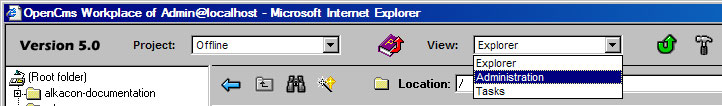
\includegraphics[width=\sgw]{pics/modules/import0}
\end{center}
\end{figure}

\item Select the {\em Online} project in the {\em Project} selection:
\begin{figure}[hbt]
\begin{center}
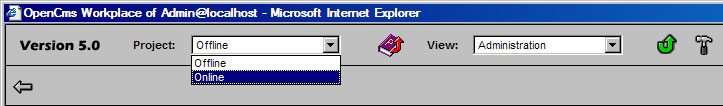
\includegraphics[width=\sgw]{pics/modules/import1}
\end{center}
\end{figure}

\item Open the {\em Module management}.

\item Click the {\em Upload module from} icon:
\begin{figure}[hbt]
\begin{center}
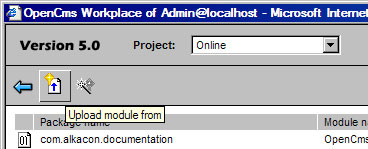
\includegraphics[width=\sgw]{pics/modules/import2}
\end{center}
\end{figure}

\item The module import wizard starts. On the first page of the wizard you can choose from where you want 
to upload the module's zip file:
\begin{figure}[hbt]
\begin{center}
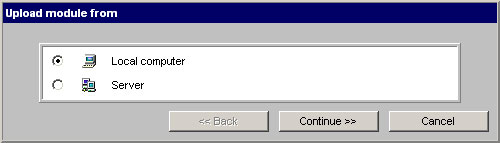
\includegraphics[width=\sgw]{pics/modules/import3}
\end{center}
\end{figure}

\begin{itemize}

\item {\em Local computer}: use this option to upload the module anywhere from your local filesystem 
(using http upload). On the next wizard page a file search dialog is shown and you can select the 
module's zip file in the local file system of your computer. 

\item {\em Server}: use this option to upload the module from the {\tt WEB-INF/export/modules/} directory of 
your OpenCms web application on the server.
On the next wizard page you get a selection with the package names of all modules found in 
{\tt WEB-INF/export/modules/} to choose from. 

\end{itemize}

\item Finally, click {\em Continue}. The import starts, reporting which files and folders are imported.

\item You might get an error or exception message during the import that tells you that you should do a 
restart afterwards. If so, do what you are told, and restart the OpenCms server after the last step. Be 
aware that you might have to restart the OpenCms server even if no such message is shown, see below for 
more details.

\item After you have left the import dialog the wizard ends and you should find the imported module in 
the list of all modules. 

\end{itemize}

{\bf Please note:} Some modules contain Java archives (JARs), class files or other resources that are automatically 
copied to the WEB-INF/classes/ or WEB-INF/lib/ folder of the OpenCms web application during the module import. 
Such modules sometimes require a restart of the OpenCms Servlet container so that the Java Classloader can 
load these new classes or resources.

The individual module documentation should contain a note if a module requires a server restart after 
installation. You will not always get an exception message during import if the module requires a server 
restart. In case you upload several modules, one server restart is usually enough after uploading all modules.

\section{How to create, administrate and export a module}

For a detailed description about the

\begin{itemize}

\item creation of a new module

\item administration of an existing module

\item distribution of a module with the export function 

\end{itemize}

please import the OpenCms interactive documentation module {\tt com.alkacon.documentation.documentation-modules}.
See the introduction chapter of this document on how and where to obtain this module.
\chapter{Usermanual}

\section{Introduction}

\subsection{What is OpenCms?}

OpenCms 5 is a Content Management System that is based on Open
Source Software. Complex Intranet and Internet websites can be
quickly and cost-effectively created, maintained and managed.

OpenCms enables you to create complete websites offline that are
published when you're satisfied with the results. An offline
project enables several users with different permissions to work
on the offline version as a team. OpenCms enables you to easily
coordinate users that are writing, designing or managing content.
It also enables you to manage the project's workflows.

Once it has been completed and approved, the offline version is
published by the project manager. Subsequent modifications and
maintenance activities are performed offline. The site is updated
by replacing the online files with the files that were modified
offline.

\subsection{The advantages of OpenCms}

OpenCms is platform independent. The software used to create the
website is installed on a web server and is accessed via the
Internet from any location such as your home. Users use their web
Browser to access OpenCms via the Internet. The combination of
their user name and password ensures that their work environment
remains protected. All of the web server's software components are
based on Java technology.

\subsection{Configuring the client}

Netscape Navigator or Microsoft Internet Explorer must be
installed on the client. You should use IE 5.5 or higher or
Netscape Navigator 7.0 or higher. Configuration details for each of
the Browsers can be found in chapter \ref{browsersettings}. 

We divided the user's guide, which explains how to use the system's
most important functions, into two parts: Part 1 consists of a
demo that is intended to give you a practical introduction to
OpenCms; Part 2 describes the individual functions of OpenCms 
more detailed.

\textbf{NOTE:} Our explanations are based on the assumption that
OpenCms has been successfully installed and is running on your web
server or local computer.
\newpage
\section{Part 1: OpenCms - The demo}

The following demo is based on a real life scenario and was
designed to get you up and running as quickly as possible.
The module \texttt{org.opencms.welcome} must be present in your OpenCms system
(it is installed per default by the OpenCms setup).

Open your Internet browser and enter

http://localhost:8080/opencms/opencms/index.jsp

to access the OpenCms welcome site.

The OpenCms site welcome page is displayed (Figure~\ref{demopage01}). The navigator on top contains
the links to all of the pages. Click on "Release notes".

The release notes page is displayed. The first
part of the demo consists of modifying this page in OpenCms by
following the instructions described below.

\begin{figure}[!hbt]
\begin{center}
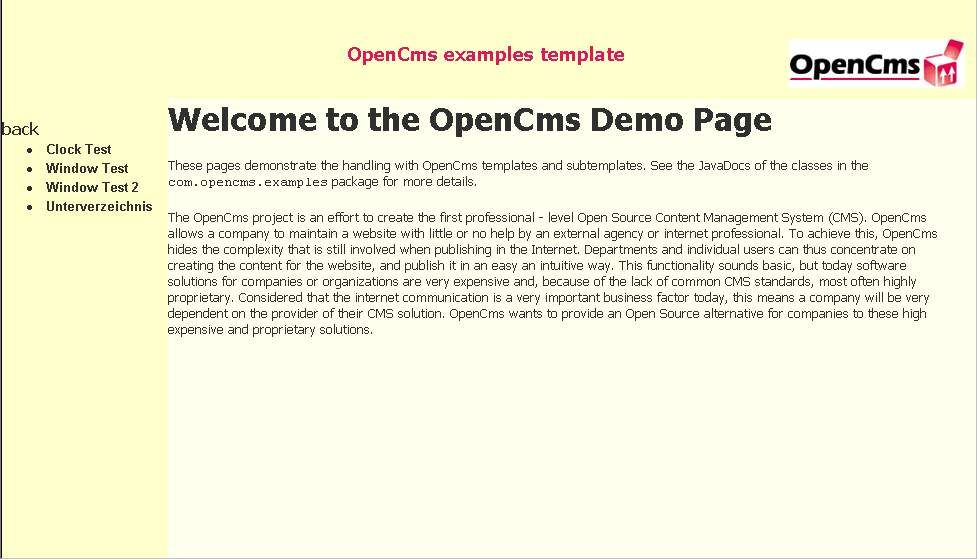
\includegraphics[width=\sgw]
                   {pics/usermanual/demoPage01}
\caption[Welcome page]
           {Welcome page}
\label{demopage01}
\end{center}
\end{figure}

\subsection{Editing a website}

Activate the "Workplace" to edit a page in OpenCms. The
"Workplace" is the OpenCms user interface that is used to change,
delete and create new pages. The "Workplace" is entirely based on
HTML, which is why you don't have to install additional software
to run it from your Internet browser.

Enter the following address in your browser to start the
"Workplace:"

http://localhost:8080/opencms/opencms/system/login/

\subsubsection{Logging into the system}

In the login dialog box (Figure~\ref{loginbox}), enter "Admin" as
the user name and "admin" as the password.

\begin{figure}[!hbt]
\begin{minipage}[b]{0.35\linewidth}
   \begin{center}
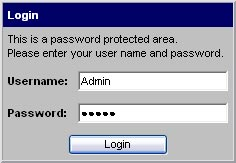
\includegraphics[width=\sgw]
                   {pics/usermanual/loginBox}
\caption["Login" dialog box]
           {"Login" dialog box}
\label{loginbox}
   \end{center}
\end{minipage}
\hfill
\end{figure}

Logging in automatically opens a new browser window and closes the
old one (you will be prompted to confirm this action). You are now
in the ``Workplace," in the so-called ``Explorer" view
(Figure~\ref{explorer}). This is where the actual editing starts.

\begin{figure}[!hbt]
\begin{center}

\includegraphics[width=\sgw]
                   {pics/usermanual/explorer}
\caption[Explorer view]
           {Explorer view}
\label{explorer}
\end{center}
\end{figure}

\textbf{NOTE:} OpenCms is a project based application, which means
that you cannot modify the pages online. You first have to create
an editing (offline) project. The default ``Offline" project can 
also be used for editing pages.

\subsubsection{Creating a new project}

Switch to the administration window by clicking on ``View" on the
menu bar and selecting ``Administration" from the drop-down menu
(Figure~\ref{view}).

\begin{figure}[!hbt]
\begin{center}
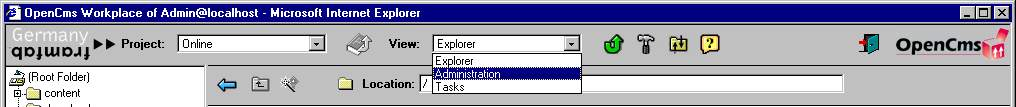
\includegraphics[width=\sgw]
                   {pics/usermanual/view}
\caption[Drop down menu ``View"]
           {Drop down menu ``View"}
\label{view}
\end{center}
\end{figure}

The Administration view is opened. The following buttons are
displayed: (Figure~\ref{adminview}):

\begin{figure}[!hbt]
\begin{center}
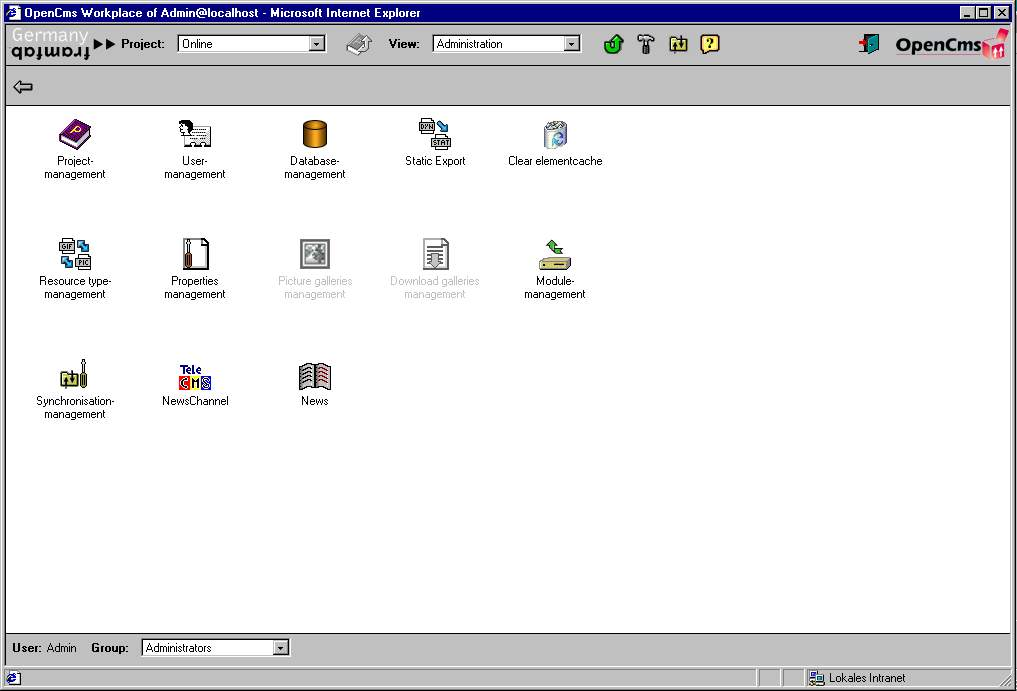
\includegraphics[width=\sgw]
                   {pics/usermanual/adminView}
\caption[``Administration" view]
           {``Administration" view}
\label{adminview}
\end{center}
\end{figure}

Click on ``Project Management." A new page is opened that contains
the following buttons (Figure~\ref{projectmanager}):

\begin{figure}[!hbt]
\begin{center}
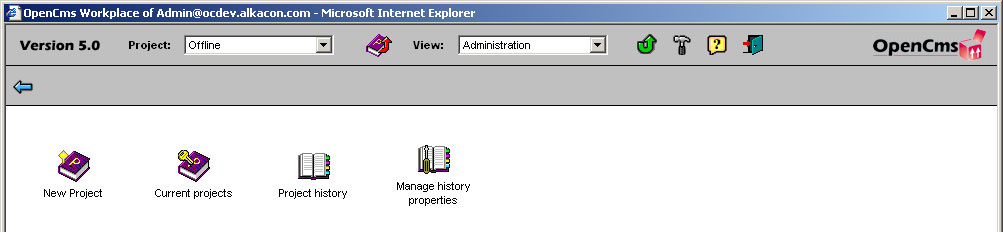
\includegraphics[width=\sgw]
                   {pics/usermanual/projectManager}
\caption[Project Management buttons]
           {Project Management buttons}
\label{projectmanager}
\end{center}
\end{figure}

Click on ``New Project" to create a new project.

The dialog window ``Create a new project" is opened
(Figure~\ref{createnewproject}). Enter the project data:

\begin{itemize}
\item Project name: Nice try
\item Description: Create test project
\item Folders: /release/
\item Channels: [leave empty]
\item User group: Users
\item Manager group: Project manager
\end{itemize}

Click on the "OK" button.

\textbf{NOTE:} Clicking on the folder icon next to the
``Directories" field opens a second window that contains a list of
the existing directories. Here you can select other directories for your
new project. The window closes automatically.

\begin{figure}[!hbt]
\begin{center}
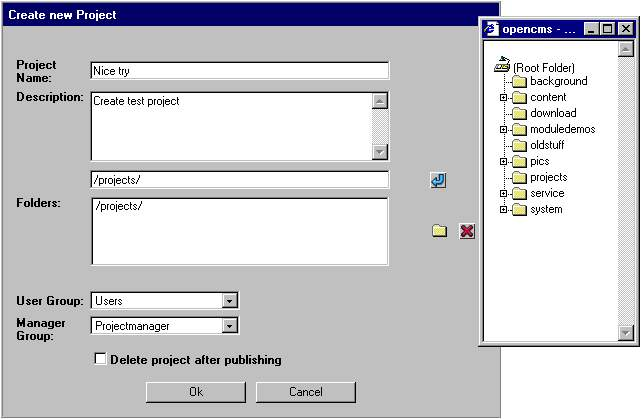
\includegraphics[width=\sgw]
                   {pics/usermanual/newProject}
\caption[Dialog window ``Create a new project"]
           {Dialog window ``Create a new project"}
\label{createnewproject}
\end{center}
\end{figure}

Switch back to the Explorer view by selecting it from the ``View"
drop-down menu. Select the ``/release/" directory (the same one you
selected when creating your project) from the drop-down menu. The
Explorer view is opened. Open your ``Nice try" project by selecting
it from the Project drop-down menu on the menu bar
(Figure~\ref{projectview}).

\begin{figure}[!hbt]
\begin{center}
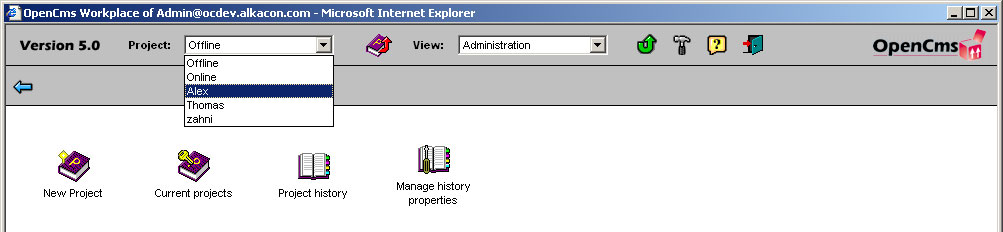
\includegraphics[width=\sgw]
                   {pics/usermanual/projectView}
\caption["Project" view]
           {"Project" view}
\label{projectview}
\end{center}
\end{figure}

The view for your project is open. You can now edit any one of its pages.

\textbf{NOTE:} You have surely noticed that all of the folders in
the folder tree are inactive except for ``/release/", ``/system/galleries/download/",
``/system/galleries/pics/", ``/system/galleries/externallinks/", 
``/system/galleries/htmlgalleries/" and ``/system/bodies/". 
Once the project is selected, OpenCms only allows you to modify files in your project directories.

\subsubsection{Editing pages}

A page must be locked for all other users before it can be opened.
Click on the icon next to the text "installation.html" with the left
mouse button to display the context-sensitive menu
(Figure~\ref{lockpage}). Click on the menu item "Lock."

\begin{figure}[!hbt]
\begin{center}
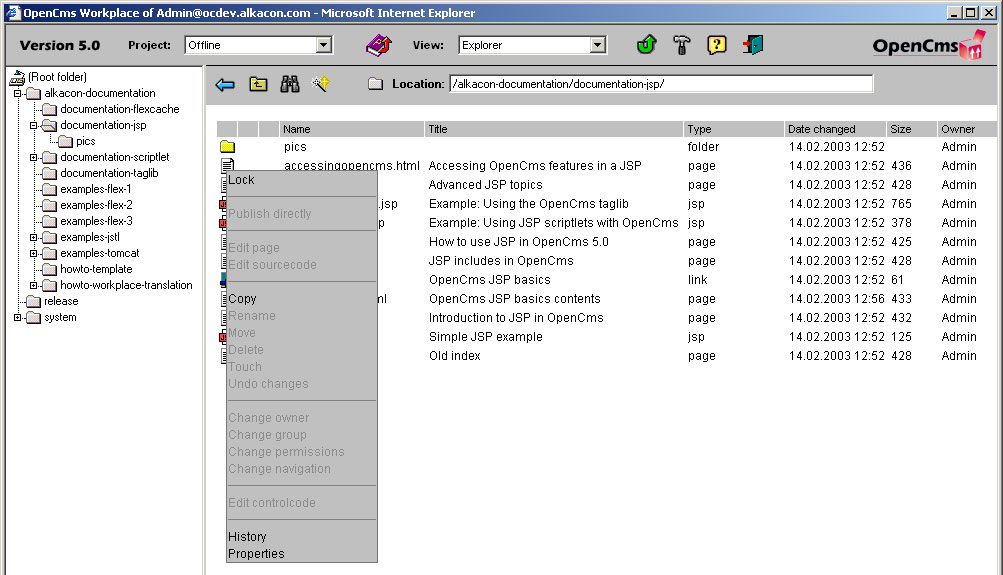
\includegraphics[width=\sgw]
                   {pics/usermanual/pageMenuUnlocked}
\caption[Context-sensitive menu]
           {Context-sensitive menu}
\label{lockpage}
\end{center}
\end{figure}

An open lock is displayed next to your locked file. Should the

\includegraphics{pics/usermanual/ic_locked}
icon not appear, check your browser settings (see above) or
refresh the view with the button

\includegraphics{pics/usermanual/ic_refresh}.

Click on the icon next to the text "installation.html" with the left
mouse button again to display the context-sensitive menu. Click on
"Edit page" to open the HTML editor.

\subsubsection{Working with the HTML editor}

You are now in the OpenCms HTML editor (Figure~\ref{htmleditor}).
Here you will find a number of editing icons that should be
familiar from other applications, such as Open Office or Word.

\begin{figure}[!hbt]
\begin{center}
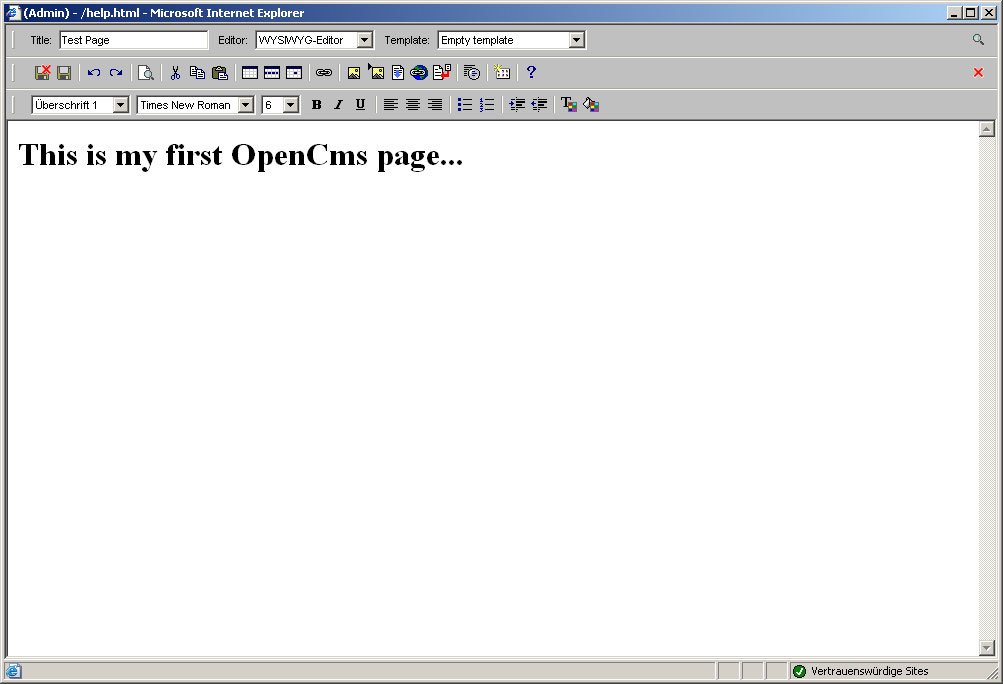
\includegraphics[width=\sgw]
                   {pics/usermanual/htmlEditor}
\caption[OpenCms HTML editor]
           {OpenCms HTML editor}
\label{htmleditor}
\end{center}
\end{figure}

In the text editor, which is just below the icons, the text that
you saw at the release notes page is
displayed. Make changes to the text and its format (e.g. bold, italics,
underline).

\textbf{By the way:} The HTML editor view you are currently in is
a WYSIWYG view (``\textbf{W}hat \textbf{y}ou \textbf{s}ee
\textbf{i}s \textbf{w}hat \textbf{y}ou \textbf{g}et"); this means
that pages are displayed here exactly as they will be seen later
on the Internet.

The "Template" drop-down menu is on the right part of the menu bar
(Figure~\ref{selecttemplate}). Select one of the pre-defined page
structures and layouts. You will see the changes by clicking on
the "preview" button in the upper right corner of the editor.

\begin{figure}[!hbt]
\begin{center}
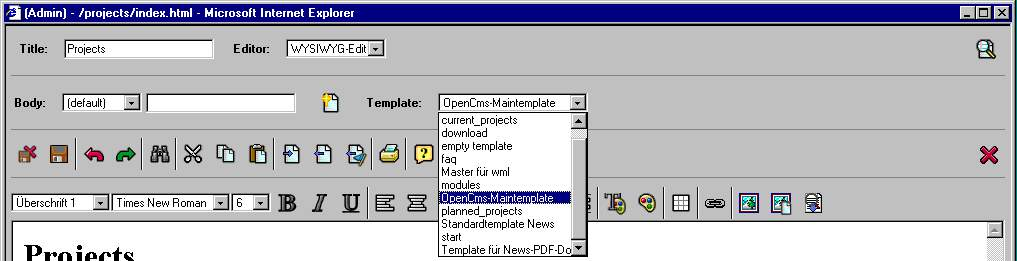
\includegraphics[width=\sgw]
                   {pics/usermanual/selectTemplate}
\caption[Drop-down menu "Template"]
           {Drop-down menu "Template"}
\label{selecttemplate}
\end{center}
\end{figure}

In the upper menu bar is the "Editor" drop-down menu, which
contains a selection of Editor views. You are currently in the
WYSIWYG view. Select the ``Sourcecode editor" view. The view is opened and
displays the same content as source code. Close the view by
clicking on the button ``Save \& Exit"

\includegraphics{pics/usermanual/ic_saveexit}, which is at the far
left of the menu bar.

The Explorer view is displayed.

\subsubsection{Completing the editing phase}

The page's details are currently displayed in red, which means
that the page has been edited. Additionally there is a little red
flag, which means that this page was locked and changed in the
current project. Click on the page icon of ``installation.html" with the left mouse to ``unlock" it. Click on
the menu item ``Unlock" in the context-sensitive menu to unlock the
page. The lock disappears (Figure~\ref{unlockpage}).

\begin{figure}[!hbt]
\begin{center}
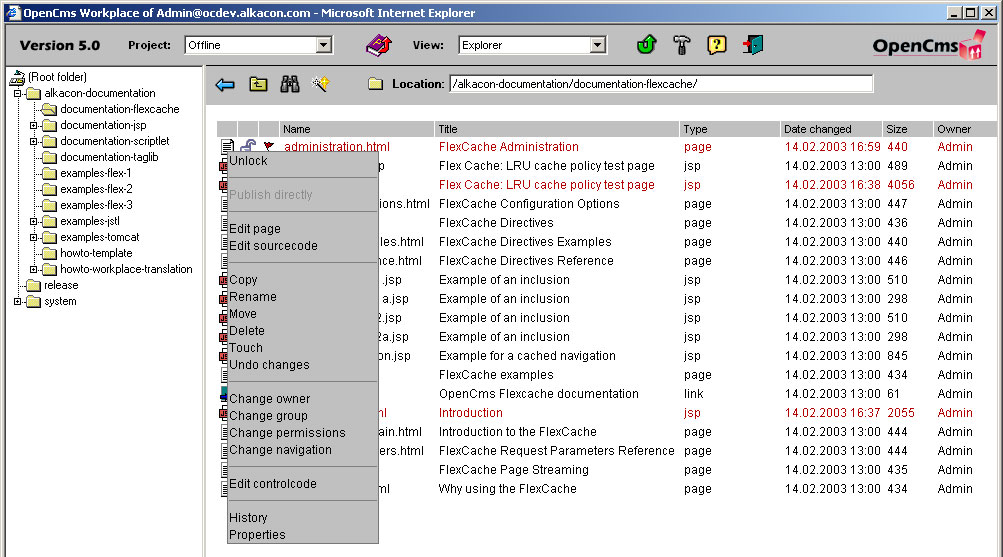
\includegraphics[width=\sgw]
                   {pics/usermanual/unlockPage}
\caption[Unlock an edited page]
           {Unlock an edited page}
\label{unlockpage}
\end{center}
\end{figure}

\subsubsection{Publishing a project}

Open the ``Administration" view. Click on the ``Project management"
button and after that on ``Current projects." The project you just edited
is displayed in the overview. Click on the project's icon to
access the context-sensitive menu. Select the menu item "Publish"
(Figure~\ref{publishproject}). Click on "OK."

\begin{figure}[!hbt]
\begin{center}
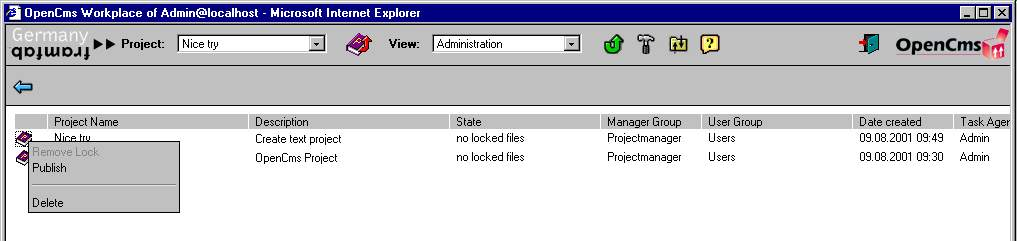
\includegraphics[width=\sgw]
                   {pics/usermanual/publishProject01}
\caption[Publishing a project]
           {Publishing a project}
\label{publishproject}
\end{center}
\end{figure}

\textbf{Note:} You can also publish the current project by clicking on the
icon between the project selector and the view selector on top of the OpenCms workplace.

Start the demo application again:\\
http://localhost:8080/opencms/opencms/release/installation.html.\\
The test page is displayed with your modifications (Figure~\ref{demopage02}).

\begin{figure}[!hbt]
\begin{center}
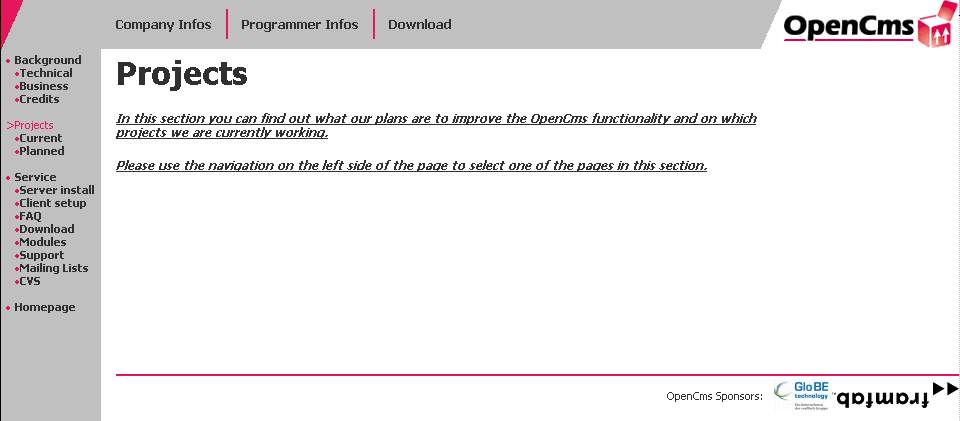
\includegraphics[width=\sgw]
                   {pics/usermanual/demoPage02}
\caption[Modified installation page]
           {Modified installation page}
\label{demopage02}
\end{center}
\end{figure}


\subsection{Creating a new page}

You can add new pages and folders for your web page from the
Explorer view. Create a new project or select the ``Nice try" project by following the steps
described above. Go to the ``/release/" directory by clicking on the
appropriate folder in the directory tree with the left mouse
button.

Click on the ``new" icon

\includegraphics{pics/usermanual/ic_newres}. The dialog window
``New" is opened (Figure~\ref{newpage01}).

Click on the radio button ``Page."

\begin{figure}[!hbt]
\begin{center}
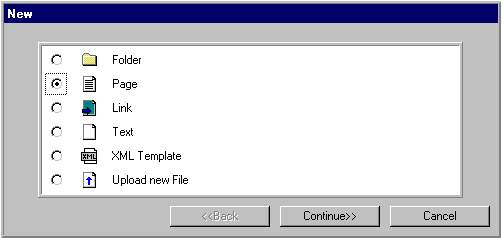
\includegraphics[width=\sgw]
                   {pics/usermanual/newPage01}
\caption[Dialog window ``New"]
           {Dialog window ``New"}
\label{newpage01}
\end{center}
\end{figure}

Click on the ``Continue" button. Enter the following data in the
dialog window ``Create a new page" (Figure~\ref{newpage02}):

\begin{itemize}
\item Name: help
\item Title: Test page
\item Template: Welcome / Release notes template
\item Keywords: Here you can enter some keywords
\item Description: Here you can enter a description
\item (Checkbox) add to navigation: check (default)
\item Text in Navigation: Help
\item Insert after: at the last position
\end{itemize}

\begin{figure}[!hbt]
\begin{center}
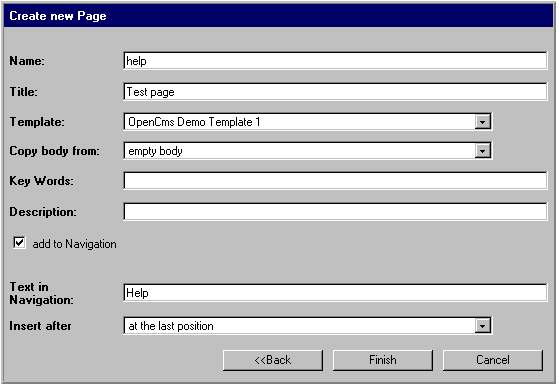
\includegraphics[width=\sgw]
                   {pics/usermanual/newPage02}
\caption[Dialog window ``Create a new page"]
           {Dialog window ``Create a new page"}
\label{newpage02}
\end{center}
\end{figure}

\textbf{NOTE:} The ``Text in navigation" is the name that will
later be displayed as the link in the online navigator.

Click on ``Finish". This takes you back to the Explorer view and
displays the details of your new page in blue with a lock
(Figure~\ref{explnewpage}). You can either continue editing the
page (see above) or use the context-sensitive menu to unlock it
for other users.

\begin{figure}[!hbt]
\begin{center}
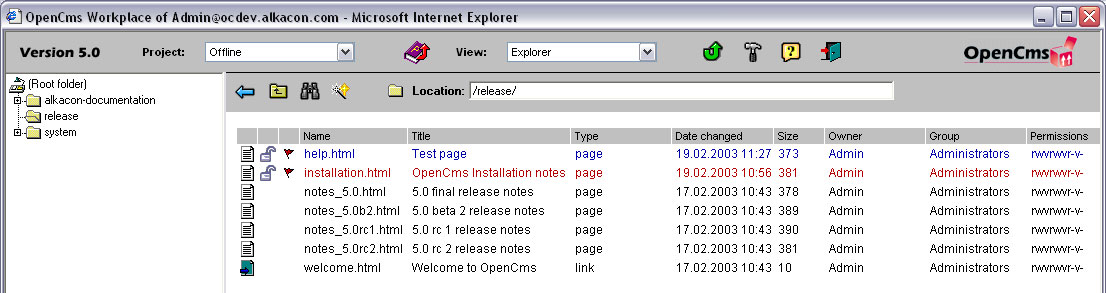
\includegraphics[width=\sgw]
                   {pics/usermanual/explNewPage}
\caption[Explorer view with new page]
           {Explorer view with new page}
\label{explnewpage}
\end{center}
\end{figure}

Publish the project as explained under ``Publishing a project" and
open the installation page:\\
http://localhost:8080/opencms/opencms/release/installation.html

The installation page is displayed with the new link to your page ``help.html" in the top navigation.
Click on the link to
view your new page (Figure~\ref{demopage03}). 

\begin{figure}[!hbt]
\begin{center}
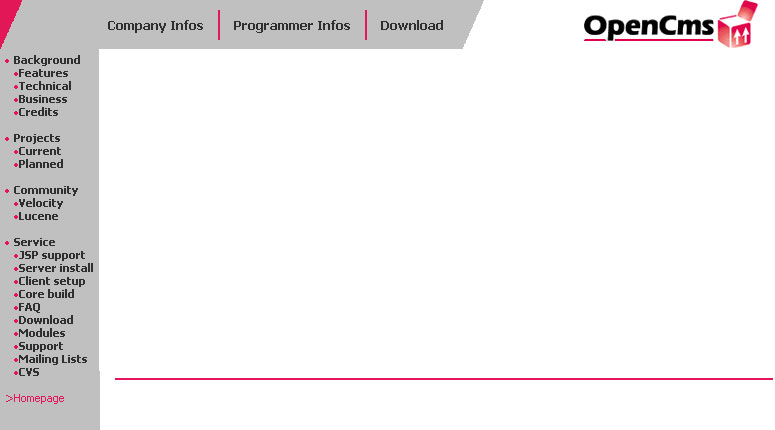
\includegraphics[width=\sgw]
                   {pics/usermanual/demoPage03}
\caption[New help page listed in navigation]
           {New help page listed in navigation}
\label{demopage03}
\end{center}
\end{figure}

This is the end of our short demo. Thank you for your attention. Additional and more detailed information about OpenCms is described in Part 2 of the guide.
\newpage
\section{Part 2: OpenCms - The mechanics}

\subsection{The user interface}
The user interface is customized by clicking on the ``Settings" tab
(the ``hammer" button 
\includegraphics{pics/usermanual/ic_settings}
on the menu bar):

\begin{itemize}
\item The additional file information that is to be displayed in the Explorer view is defined on the ``Explorer" tab.
\item The Standard view and messaging options for task management are defined on the ``Tasks" tab.
\item The user's default startup settings and permissions for new files are defined on the ``Startup Options" tab.
\item A user's group and password are changed on the ``User Data" tab.
\end{itemize}

\subsection{View Modes}

The user screen contains all of the components, grouped in views,
that enable users to create, maintain and manage web pages. In the
``Explorer" view, users manage directories and files and edit HTML
pages. A project's workflow is managed in the ``Tasks" view. Users,
groups, projects, database connections, images, documents etc. are
managed in the ``Administration" view. The user screen (default
startup view) is started via a login dialog and is displayed as a
file explorer. The directory tree structure, the file view and the
menu bar make it easy for users to access files and functions
(Figure~\ref{workplace}) :

\begin{figure}[!hbt]
\begin{center}

\includegraphics[width=\sgw]
                   {pics/usermanual/workplace}
\caption[User screen]
           {User screen}
\label{workplace}
\end{center}
\end{figure}

Users can switch between the online version of the web page and
the individual offline projects by selecting one of the options in the
``Project" drop-down menu.

Users can switch between the ``Explorer", ``Tasks" and
``Administration" views by selecting one of the options in the
``View" drop-down menu.

The files and directories are managed via a context-sensitive menu
that is activated by clicking on the file or directory icon in the
file overview.

The content of the website as it will be seen online is displayed
in the browser screen (Figure~\ref{browserscreen}). The website's
files and directories cannot be modified in the online version.
The browser screen, which displays the page as it would be seen by
someone visiting the live site, is activated by clicking on the
file name in the ``Explorer" view:

\begin{itemize}
\item The Template of an OpenCms-generated browser page contains the
static and dynamic navigation components as well as other dynamic
components such as logos or text fields that can be freely
defined. The template determines the page's layout.
\item The content is displayed in the Body. Content is freely defined. Its
layout is based on previously defined format templates. The format
templates ensure that the content is uniformly displayed.
\end{itemize}

\begin{figure}[!hbt]
\begin{center}
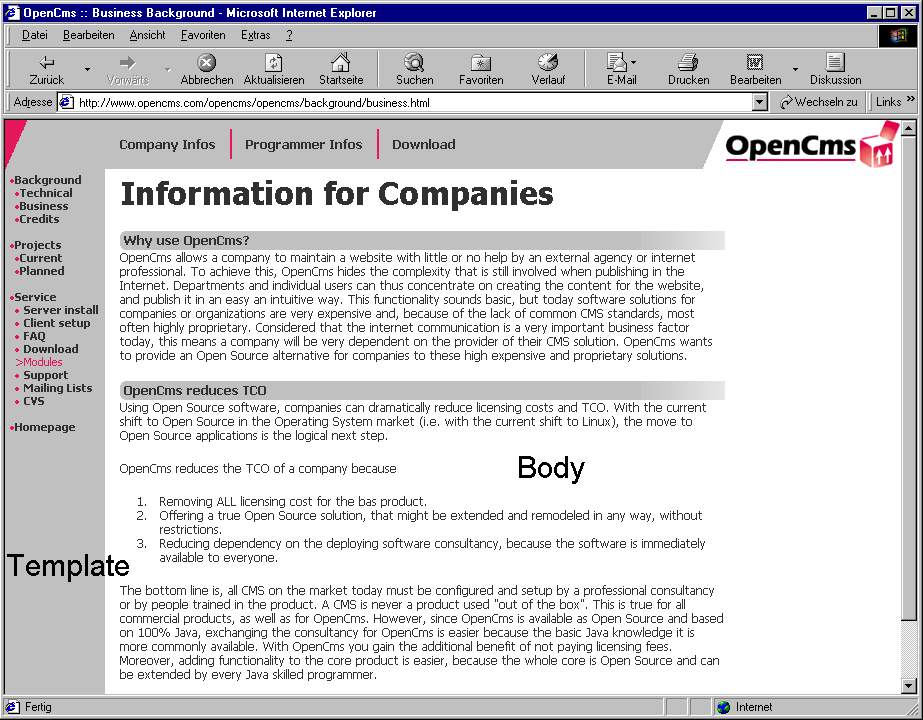
\includegraphics[width=\sgw]
                   {pics/usermanual/browserScreen}
\caption[Browser screen]
           {Browser screen}
\label{browserscreen}
\end{center}
\end{figure}

\subsection{Working on a project}

An offline project is created by a user that belongs to the
"Project manager" group. The project can be created for an
existing website that needs updating or a brand new website.

When you create an offline project for an existing website a view
on the offline resources for this website is created. When the
modified pages are published, the changes are copied to the online
project. Additionally the changed resources are stored in backup
tables for traceability purposes.

By default, an offline project's files and directories can only be
modified by the project members. Responsibilities are clearly
defined by assigning specific users and groups to specific files
and directories. It is also possible to process part of the web
site in different projects at the same time. Locking and unlocking
functions ensure that access security remains intact for larger
user groups.

The modifications that are made to the files are written to a
backup table after publishing. The information about all versions can
be accessed via the ``History" option in the context-sensitive menu
(Figure~\ref{history01}).

\begin{figure}[!hbt]
\begin{center}
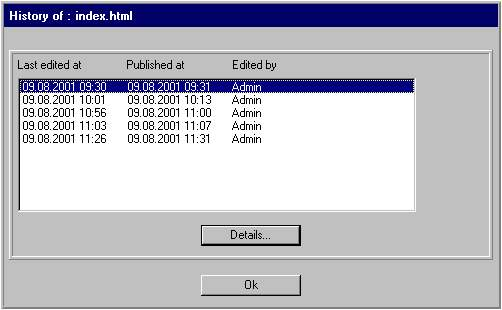
\includegraphics[width=\sgw]
                   {pics/usermanual/history01}
\caption[Project history]
           {Project history}
\label{history01}
\end{center}
\end{figure}

To create new content, the user creates a new file or directory by
clicking on the ``New" button on the menu bar. This opens a dialog
window in which the user selects the element to create: ``Folder,"
``Page," ``Link", ``Text", ``XMLTemplate", ``JSP" or ``Upload new file." The
name, title and navigation text as well as the position of the file
or directory in the navigation, are defined in separate dialog
boxes. Selecting the option ``Upload new file" enables users to load
files that are stored on their PC's local hard disks into an
OpenCms directory. Users access their assigned directories and
files via the file ``Explorer" view of OpenCms.

Clicking on the directory name (e.g. ``OpenCms") in the directory
tree structure or in the ``Explorer" view displays the directory's
contents. Clicking on an HTML file name (e.g. ``index.html") opens
a preview of the file in the Internet browser. Clicking on a directory or file
icon (text file, image etc.) in the file overview displays a
context-sensitive menu. The menu contains the following functions
that are accessible (active/inactive) based on the file's or
directory's status and the user's access permissions:

\begin{itemize}
\item \textbf{Lock or Unlock}: Directories or files can be locked throughout
the editing phase to prevent them from being accessed or modified
by several users at the same time. A file or directory is unlocked
when the user has finished modifying it.

\item \textbf{Publish directly}: A single resource can be published
directly. This item is enabled when a changed file is unlocked.

\item \textbf{Edit page}: Clicking opens a WYSIWYG editor in which the file can be modified.
At this stage, no HTML knowledge is required to modify a page.

\item \textbf{Edit sourcecode}: Clicking opens a text editor in which the file can be modified.
This requires at least basic HTML knowledge to modify a page.

\item \textbf{Edit control code}: Clicking opens a text editor in which
control codes can be edited.
\textbf{Warning:} Extensive knowledge of the OpenCms template mechanism is required
to make modifications of this type.

\item \textbf{History}: The history file displays all of the file's previous
versions. The history file enables users to see who made which
modifications when. When the file is locked a button for restoring
a version is shown in the ``Detail" of the version.

\item The respective access
attributes for the individual files and directories are set on the
system side by using the functions ``\textbf{Change owner}", ``\textbf{Change group}"
and ``\textbf{Change permissions}".

\item \textbf{Change navigation}: Here the navigation text and position of a resource can be changed.

\item \textbf{Properties}: To every resource properties can be attached as key / value pairs, 
e.g. the title or the description is stored as a resource property.
Properties can be added, modified or deleted.

\item Standard functions such as ``\textbf{Copy}",
``\textbf{Rename}", ``\textbf{Move}" and ``\textbf{Delete}" can be selected from the context
menus. ``\textbf{Touch}" changes the timestamp of a resource, which marks it as changed, 
and it will be published when the project is published.

\item \textbf{Undelete resources}: \index{undelete} When a resource
that already exists in the online project is deleted it is marked
by crossing out its entry in the file list. Now it is possible to
undelete these resources. When undeleting a folder all
subresources in this folder that were marked as deleted are
undeleted, too. You must have write access to undelete a resource.

\begin{figure}[!hbt]
\begin{center}
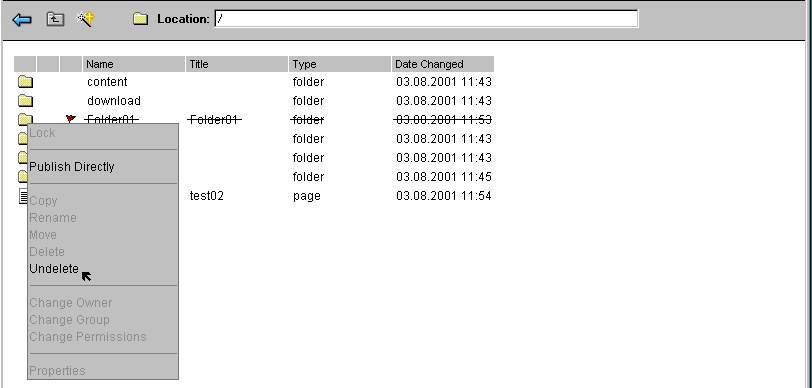
\includegraphics[width=\sgw]
                   {pics/newProject/undel03}
\caption[Undelete a resource]
           {Undelete a resource}
\label{undel}
\end{center}
\end{figure}

After the resource is undeleted its state is set to changed and
the resource is locked by the current user.


\item \textbf{Undo changes}  \index{undo}

Changes of a resource can be undone. The resource must be
marked as changed and it must be locked. You must have write
access to the resource. When the changes of a folder are undone
all changes of subresources are undone, too. This feature copies
the information from the online project, so all changes that were
not published yet are lost and new resources are deleted.

\begin{figure}[!hbt]
\begin{center}
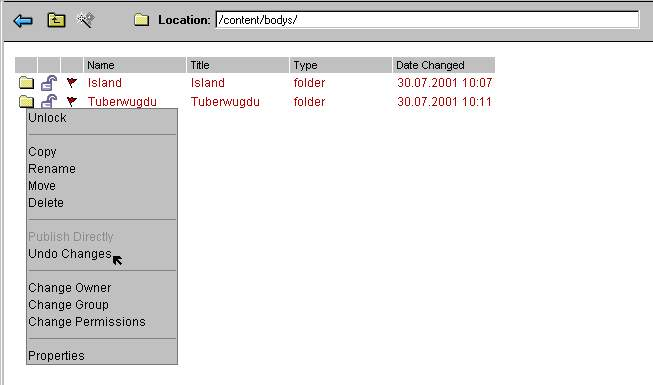
\includegraphics[width=\sgw]
                   {pics/newProject/undo01}
\caption[Undo changes of a resource]
           {Undo changes of a resource}
\label{undo}
\end{center}
\end{figure}


\item \textbf{Restore a version from history}  \index{history}

Older versions of a file can be restored from the history. The
file must be locked. This feature currently works only for files,
not for folders. The function is only enabled for locked files. It
is implemented in the detail view of the history.

You have to choose the version from the list of versions and click
on the detail button. To restore the version click on the ``Restore
version"-button. You must have write access to the file if you
want to restore a version.

\begin{figure}[!hbt]
\begin{minipage}[b]{0.49\linewidth}
\begin{center}
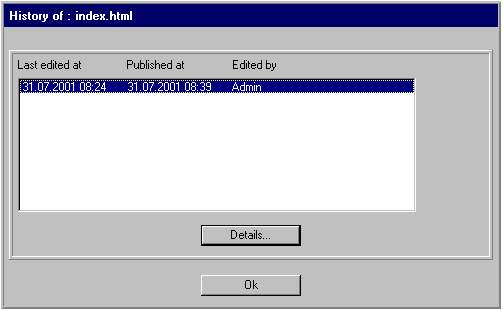
\includegraphics[width=\sgw]
                   {pics/newProject/restore01}
\end{center}
\end{minipage}
\begin{minipage}[b]{0.49\linewidth}
\begin{center}
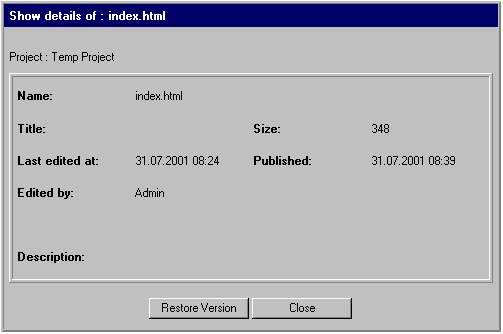
\includegraphics[width=\sgw]
                   {pics/newProject/restore02}
\end{center}
\end{minipage}
\caption[Restore a version]
           {Restore a version}
\label{restorever}
\end{figure}


\item \textbf{Publish a resource} \index{publish resource}

Resources can be published directly. They must be unlocked to
enable the function in the context menu. Only members of the projectmanager
and the administrator groups are allowed to publish resources of a project.

\begin{figure}[!hbt]
\begin{center}
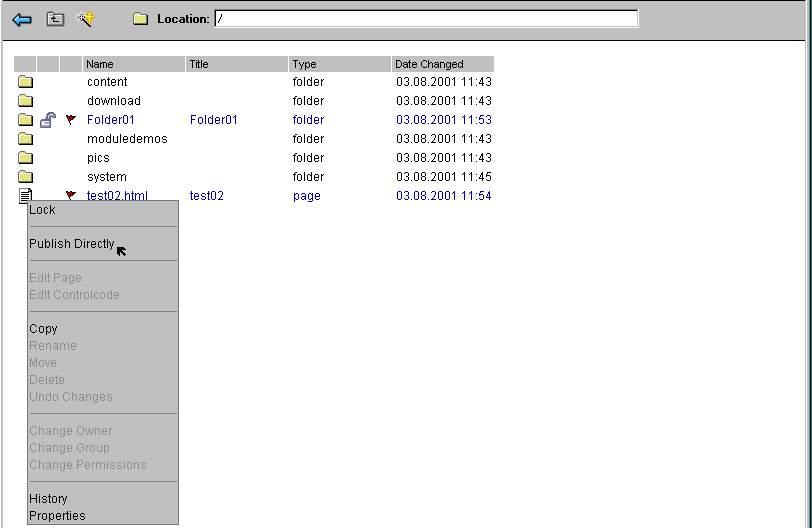
\includegraphics[width=\sgw]
                   {pics/newProject/publish03}
\caption[Publish a resource]
           {Publish a resource}
\label{publishres}
\end{center}
\end{figure}

When a resource is published directly

\begin{itemize}
\item a temporary project is created
\item the resource is copied to the new project
\item the projectid of the resource and all its subresources is set to the new project
\item the new project is published and deleted.
\end{itemize}


\item \textbf{Copy a resource to the project}

A resource that does not belong to the current offline project is
colored grey. You can copy this resource to the current offline
project with this new feature in the context menu. Only the
projectmanager and the administrator are allowed to copy resources
to the project.

\begin{figure}[!hbt]
\begin{center}
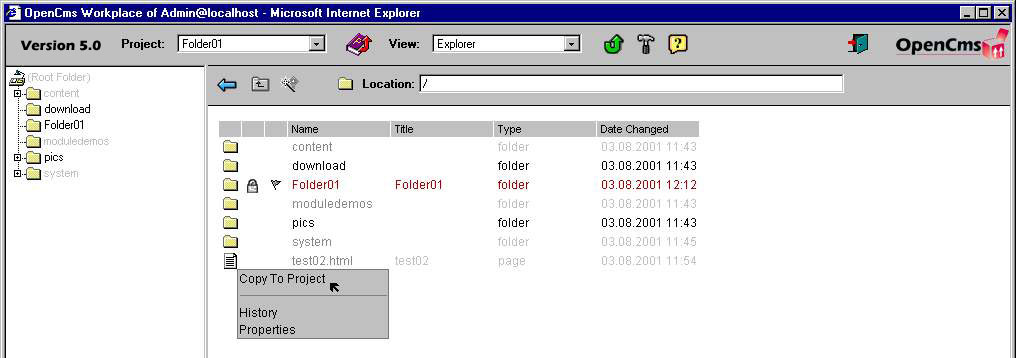
\includegraphics[width=\sgw]
                   {pics/newProject/copyPro02}
\caption[Copy a resource to project]
           {Copy a resource to project}
\label{copytoproject}
\end{center}
\end{figure}

You can also copy the parent resource of an already existing
resource to the project, but it is not possible to copy the root
folder to an existing project. For this you must create a new
project.

\end{itemize}

\subsection{Access permissions}

On the user side, different access permissions determine which
actions users can perform and which components they see, i.e.
users see only those files and directories that are relevant to
them. Doing this provides users with a well structured overview.
Each user belongs to at least one user group, but can belong to
several (Figure~\ref{newgroup}).

The following groups are pre-defined in OpenCms:

\begin{itemize}
\item \textbf{Administrators}: An administrator has full access permissions to
all of the files and directories. Administrators create and manage
users and user groups.
\item \textbf{Projectmanager}: A project manager creates new projects and coordinates their workflow. A project manager's access permissions are restricted to the projects he/she creates. A project manager can, however, access all of the files and directories within his/her projects. A project manager can also publish projects, i.e. put them online.
\item \textbf{Users}: A user can create new files and directories within the project he/she is assigned to. As the owner, the user has full access permissions to the files and directories he/she creates.
\item \textbf{WebUsers}: Webusers cannot login in the OpenCms workplace, but can have access to restricted areas of a website which is forbidden for Guests.
\item \textbf{Guest}: This group consists of all other users, such as visitors.
\end{itemize}

Based on the requirements, additional groups such as editors,
designers, testers etc. can be created.

\begin{figure}[!hbt]
\begin{center}
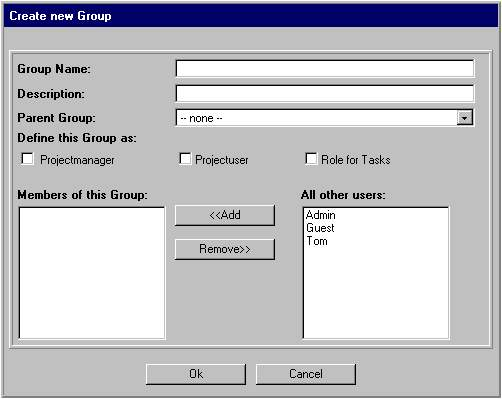
\includegraphics[width=\sgw]
                   {pics/usermanual/newGroup}
\caption[Create a new group]
           {Create a new group}
\label{newgroup}
\end{center}
\end{figure}

On the system side, each file and each directory is assigned to
one user, which by default, is the user that created the file or
directory, making him/her its owner. Each file and each directory
is also assigned to one user group that has specific access
permissions. This enables the users in this group to access the
files and directories that are relevant to them. File and/or
directory attributes, such as the owner of a file or directory, or
the group assigned to the files, can only be modified by the
administrator and/or the file and/or directory owner. All access
permissions are maintained via the ``Change owner", ``Change group"
and ``Change access permissions" options in the context
menu. File and directory access permissions are classified by
``Owner permissions", ``Group permissions" and ``Other permissions." A
user's access permission can be restricted to the files and
directories that he/she owns. The following abbreviations are used
to set a user's permissions: r = read, w = write, v = visible, i =
internal.

\subsection{The editor}

The editor is used to create content in the body, which is
structured by a template that ensures that the layout for the
navigator, the content and the individual pages - basically the
layout for the whole site - is uniform
(Figure~\ref{thehtmleditor}):

\begin{figure}[!hbt]
\begin{center}
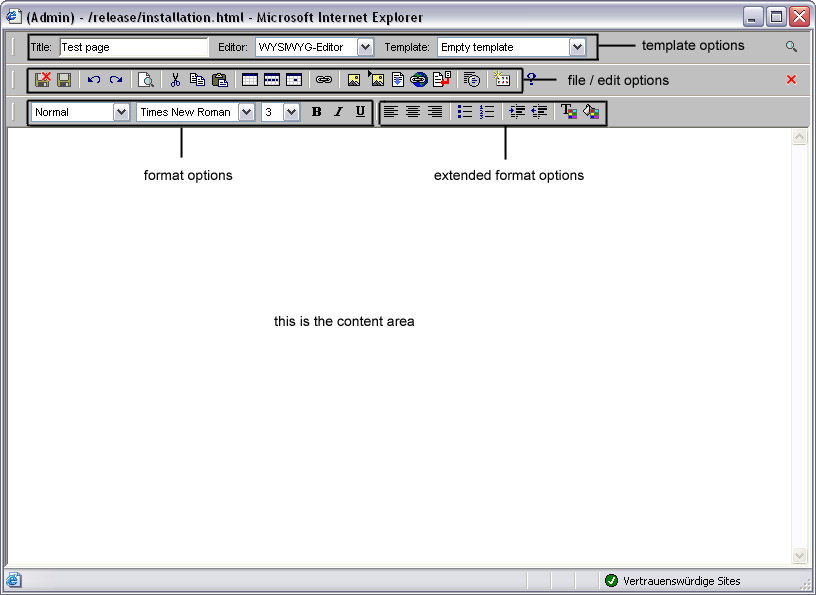
\includegraphics[width=\sgw]
                   {pics/usermanual/theHtmlEditor}
\caption[The HTML editor]
           {The HTML editor}
\label{thehtmleditor}
\end{center}
\end{figure}

The functionality of the OpenCms editor is very similar to that of
a standard WYSIWYG HTML editor with templates, tables, preview
functions, such as Netscape Composer. It is also possible to
switch between sourcecode and WYSIWYG mode. A page's layout is
determined by a template. Complex layouts are created by cascading
several templates. OpenCms is only used to edit the body of an HTML page.

\subsection{Workflow}

The project manager creates a new task and defines its role by
clicking on the ``New" button in the ``Tasks" view. A role consists
of several users that have the skills to perform a specific task
such as editing, designing graphics, writing HTML code, etc. A
preferred user is selected for each task. The name, the
definition, the due date and the priority of the task as well as
various messaging options are also defined. Depending on the
selected messaging options, an e-mail is automatically sent to
either the preferred user or all users that are assigned to a role
as soon as a new task has been added to the project. The task is
active once the appropriate user has accepted it. Optionally, the
project manager receives an e-mail when the task has been
accepted, rejected, forwarded or completed. Users can view the
tasks that have been assigned to them as well as those they have
forwarded to others by filtering on specific criteria in the
drop-down menu ``Filter" (Figure~\ref{taskview}). Different icons
and colors are also used to define a project's status. A task that
is still within the due date is shown in black. If the due date is
exceeded, the task is shown in red. A completed task is shown in
gray. A task's priority is defined by icons (low, normal and
high). The task descriptions provide a clear overview of a user's
task account.

\begin{figure}[!hbt]
\begin{center}
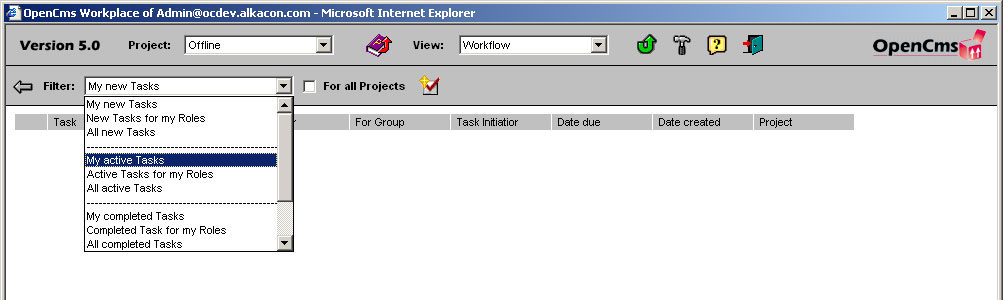
\includegraphics[width=\sgw]
                   {pics/usermanual/taskView}
\caption["tasks" view]
           {"tasks" view}
\label{taskview}
\end{center}
\end{figure}

Clicking on the name of a new task displays its details and
history. Each stage of the project is tracked and ensures that the
workflow remains transparent.

\chapter{Components used by OpenCms}
\label{components}

This chapter describes all external parts required to run OpenCms.
If you want to prepare an installation, please collect all
components listed here. If you download a major release of OpenCms
(e.g. version 5.x) the MySQL connector, Xerces, JavaMail, Fesi, 
Jakarta-ORO and JTidy will be shipped with the distribution.

\section{Operating System}
OpenCms is implemented in 100\% Java. Since Java should be platform independent, OpenCms should run
on all operating systems supporting Java. Currently, we have installations running on
Red Hat Linux 7.2 (\rqhttp{http://www.redhat.com}{http://www.redhat.com}). Other
Linux or Unix brands should work without problems. We also have installations on
Windows NT 4.0, Windows 2000 and Windows XP.

\section{Webserver}
The reference webserver for OpenCms is, of course, the excellent Apache webserver \\
(\rqhttp{http://www.apache.org}{http://www.apache.org}).
Apache is the clear market leader with more than 50\% market share,
it is used by IBM as webserver for their operating systems, and it is also Open Source and
free of charge. We have been using OpenCms with Apache since version 1.3.6 on Linux and Windows.
For Windows systems, the Microsoft IIS (\rqhttp{http://www.microsoft.com/
iis}{http://www.microsoft.com/\\
iis})
has also been successfully tested with OpenCms. 
Other web servers should also be working without problems.

\section{Servlet runtime engine}
The Java Servlet API (JSDK) 2.3 and a servlet engine are needed by
the webserver to start up Java programs on http requests. The
servlet standard has been developed by SUN, see
\rqhttp{http://java.sun.com/products/servlet/index.html}{http://java.sun.com/products/servlet/index.html}.
We are most often using TOMCAT as a Java Servlets and Java Server
Pages reference implementation from the Apache Foundation. Please use
Tomcat 4.x or later. See
\rqhttp{http://jakarta.apache.org/}{http://jakarta.apache.org/}

For a Microsoft IIS installation, we have successfully used Jrun from Allaire \\
(\rqhttp{http://www.allaire.com/Products/Jrun/}{http://www.allaire.com/Products/Jrun/}).\\
Since servlets are a standard API which is part of the J2EE specification,
other servlet engines should be working without problems.

\section{Java VM}
To run servlets, a Java Virtual Machine (VM) is needed. For development we are currently using
a version 1.4 compliant JDK, like the one provided \\
by SUN (\rqhttp{http://java.sun.com/j2se/1.4/}{http://java.sun.com/j2se/1.4/})\\
or IBM (\rqhttp{http://www.ibm.com/java/jdk/index.html}{http://www.ibm.com/java/jdk/index.html}).\\
For running systems we recommend using a Java VM version 1.4 or higher.

\section{Database}
The OpenCms architecture allows to use any SQL capable database that offers a JDBC connector.
These include enterprise databases like e.g. Oracle (\rqhttp{http://www.oracle.com}{http://www.oracle.com}),
but also Open Source databases like MySQL (\rqhttp{http://www.mysql.com}{http://www.mysql.com}).
The reference installation uses MySQL. For development we are currently using version version 3.23 of 
MySQL and version 2.0.14 of the MySQL Connector/J driver.

\section{XML Parser}
OpenCms makes heavy use of XML to store content and template data. For XML parsing, we make use of
the excellent Xerces developed by the Apache Foundation\\
(\rqhttp{http://xml.apache.org/xerces-j/index.html}{http://xml.apache.org/xerces-j/index.html}).
We recommend using version 1.4.4.

\section{Mail API}
The integrated task management is able to send mails when task events occur.
To enable this feature you will need the JavaMail 1.2 API available at \\
\rqhttp{http://www.javasoft.com/products/javamail/index.html}{http://www.javasoft.com/products/javamail/index.html}
 and the activation Java\-Bean
(\rqhttp{http://www.javasoft.com/beans/glasgow/jaf.html}{http://www.javasoft.com/beans/glasgow/jaf.html}).

\section{FESI (a Free EcmaScript Interpreter)}
OpenCms uses FESI as Interpreter for EcmaScript. This interpreter is used by OpenCms if you start the cmsshell in
ExmaScript mode.
(\rqhttp{http://home.worldcom.ch/jmlugrin/fesi}{http://home.worldcom.ch/jmlugrin/fesi})

\section{JTidy}
OpenCms uses JTidy release 7 to cleanup and parse HTML-fragments produced by the HTML-Control. 
(\rqhttp{http://sourceforge.net/projects/jtidy}{http://sourceforge.net/projects/jtidy})

\section{Jakarta-ORO}
OpenCms uses regular expressions for linkreplacements in case of static export. Therefor jakarta-oro-2.0.6.jar
is used.
(\rqhttp{http://jakarta.apache.org/oro/index.html}{http://jakarta.apache.org/oro/index.html})

\chapter{Useful resources}

\section{OpenCms online resources}

\begin{itemize}
\item Please use our OpenCms bugzilla to report bugs that you have found in OpenCms. 
Before doing so, please check if the bug that you have found is certainly a new bug:\\
{\tt http://www.opencms.org/bugzilla/}
\item The CVS web interface allows you to browse through the OpenCms sources:\\
{\tt http://www.opencms.org/cgi-bin/cvsweb.cgi/}
\item Use the OpenCms mailinglist archive to search for older postings:\\
{\tt http://www.opencms.org/cgibin/wilma/opencms-dev}
\end{itemize}

\section{How you can help}
{\bf Please report bugs}\\
You might find that someting does not work as it should. If so, you should provide a bug report. 
Please use the OpenCms Bugzilla for all of your bug reports. You might have to create a Bugzilla 
account first. Please use the Bugzilla if possible and not the "opencms-dev" mailing list to report 
bugs. If you encounter setup related problems, please post them on the mailing list first, because 
in 99.5\% of all cases setup issues are not bugs in OpenCms but related to your local environment
configuration.\\
\\
{\bf Test out the new functionality}\\
The easiest way to participate in the development process would be to help testing the JSP integration, 
the interactive documentation and other new functionality. Please use the opencms-dev mailing list for 
discussions on the development process, about this documentation or about OpenCms in general. Note: This 
mailing list requires subscription prior to posting (see below). Please use the "opencms-dev" mailing list 
for questions and comments regarding OpenCms or the documentation and not Bugzilla.\\
\\
{\bf Provide examples and demos}\\
Another way to help extending OpenCms is to provide examples and demos for the use of JSP pages in OpenCms. 
If you contribute these, we might include these in this documentation in a later release. Or we could make 
your examples available as a separare module download. The best way to distribute your new demo or example 
would be to post it to the opencms-dev mailing list or to {\tt contributions@opencms.org}.

\section{How to subscribe to the opencms-dev mailing list}
The main place for the latest OpenCms related information is the mailing list\\ {\tt opencms-dev@opencms.com}. 
This list is for all general and development related news, messages and questions regarding OpenCms.
Traffic on the list is currently about 10 messages a day (as of February 2003).

To subscribe to the list, send a message to:

{\tt majordomo@opencms.com}

and just include the text

{\tt subscribe opencms-dev \{insert-your-email-address-here\}}

in the body of your mail. The mail does not need a subject. 
{\em Please do not use the domain name opencms.org for the subscription.} We have had various complains about the 
subscription process in the past, and we might change this in the future to make it more easy. As of now, just 
make sure you follow the instructions given here to the letter, and if it does not work the first time try again.

Before posting a question to the list, you should check out the opencms-dev mailing list archive if this question 
has already been answered.


\part{Archived documentation}
\chapter{About the archived documentation}
\section{About the archived documentation}

We are currently in the process to shift the book documentation
into interactive documentation modules. During this process, the
content of the book documentation is generally revised and updated.

Not all sections of the book documentation are already available
as interactive documentation modules yet. OpenCms now supports more 
than one template mechanism, and we preach to use standard JSP templates 
instead of proprietary XML templates. Thus it would make little sense
to transform the documentation of the proprietary XML template mechanism 
into a documentation module. Instead, these chapters were moved into the
archive part of the book documentation, where we also fixed typos and 
updated system paths in the example.
\chapter {Enterprise JavaBean Integration}
\section {Advantages of OpenCms \& EJB}
Running OpenCms in an application server environment provides facilities
for making use of distributed object architectures, particularly with
regard to Enterprise JavaBeans  technonolgy. Using these techniques,
processes behind the web site may be structured and distributed in a
component oriented way. Server sided presentation logic and business
logic can be developed strictly separated, according to the four-tier
architecture described in the J2EE Application Model: OpenCms takes care
of the presentation of the data, using the integrated template engine
and master templates for displaying it in a general layout, while the
generation of the content data is relocated to the EJB (figure~\ref{EJB}).

\begin{figure}[!hbt]
\begin{center}
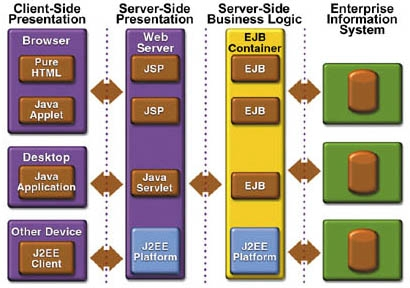
\includegraphics[clip,width=\sgw]{pics/ejb/ejb}
\end{center}
\caption[OpenCms and EJB]{OpenCms and EJB.}
\label{EJB}
\end{figure}

\index{EJB}
Implementing EJB components implicates a lot of advantages that enhance
the ease of handling with business data. This includes:

\begin {itemize}
\index{Concurrency}
\item {\bf Concurrency:}
The EJB server handles any concurrencies between EJB. The developer
doesn't have to care about threads or synchronization.
\index{Transactions}
\item {\bf Transactions:}
All set of tasks that have to be executed together will be managed by
the EJB server
\index{Persistence}
\item {\bf Persistence:}
The EJB server ensures, that any object is actually containing the most
recent data from any external database.
\index{Distributed Objects}
\item {\bf Distributed Objects:}
Clients do not have to know the exact location of Beans it is using.
This is transparent to the client. The EJB server takes care of  all
communication and remote method invocations (RMI).
\index{Naming}
\item {\bf Naming:}
The EJB server provides a service for looking up distributed objects.
This enables the client to request remote objects.
\index{Security}
\item {\bf Security:}
Authentication, access control and secure communications are ensured by
the server.
\end{itemize}

In the environment of OpenCms, EJBs may be used for different purposes,
such as plausibility checks of user input, database access or connection
to host systems. Even reuse of existing shared libraries is possible by
{\name "wrapping"} them with EJB components.

\section {EJB basics}
There are two different types of Enterprise Beans: Entity and Session
Beans. Entity Beans model real-life objects usually represented by some
records in a database. Session beans are used to map processes or tasks.
They usually operate on the data modelled by Entity Beans.
There is a further distinction between stateful Session beans, if the
Bean stores data over more than one session and stateless Session beans,
if the Bean only operates with the current parameters.
To implement an Enterprise Java Bean at least three components
are required:

\begin{itemize}
\index{Remote interface}
\item {\bf Remote interface:}
This interface contains all business methods that may be called remotely
(i.e. all methods visible from OpenCms). It has to extend EJBObject.

\index{Home interface}
\item {\bf Home interface:}
This one keeps all methods for finding, deleting or creating new EJB
objects. It must contain the create() Method for building new objects
and extends EJBHome.

\index{Bean class}
\item {\bf Bean class:}
This class implements all methods defined in the two interfaces above.
Note! Though the methods match the ones defined in the interfaces, these
are not implemented in this class.
For defining a entity bean, an additional component is required:

\index{Primary key}
\item {\bf Primary key:}
This is a class implementing a pointer to the database.
\end{itemize}

Since OpenCms only calls, but not implements EJB modules, only the two
interfaces become important at this point: They are essential for
looking up and calling an EJB.
Two sample home and remote interfaces may look as follows (these
examples are taken from the WebLogic {\name "examples" package)}:

\begin{java}
public interface TraderHome extends EJBHome \{\\
\jtaba  Trader create() throws CreateException, RemoteException;\\
\}\\

public interface Trader extends EJBObject \{\\
\jtaba  public  TradeResult buy (String stockSymbol, int shares)\\
\jtabb    throws RemoteException;\\

\jtaba  public TradeResult sell (String stockSymbol, int shares)\\
\jtabb    throws RemoteException;\\
\}\\
\end{java}


\section {Calling an EJB}
Calling an Enterprise JavaBean from OpenCms is quite easy and only
requires four steps:

\begin{enumerate}
\item   Get the {\name "initial context"}. Every Bean has a  initial context
object defining the Bean's environment containing the URL for the naming
service, the user and his password.
\item Get the EJB home. This is the implementation of the home
interface and can be used to get the EJB object.
\item Get the EJB object
\item Call any required EJB method on this object.
\end{enumerate}

In the Java code, this may look like:

\begin{java}
import javax.naming.Context;\\
import javax.naming.InitialContext;\\

Context jndiContext = getInitialContext();\\
TraderHome home = (TraderHome)jndiContext.lookup(C\_JNDI\_TRADER);\\
Trader t = home.create()\\
TradeResult res = t.buy("FFN", 100);\\
\end{java}

Instead of the buy() method every other method defined in the remote
interface could be called.
For getting the initialContext, some additional steps must be executed.
Note, that the name of the context factory is application server
dependend. This example again shows the code for the WebLogic server:

\begin{java}
protected Context getInitialContext() throws Exception \{\\
\jtaba     // Get an InitialContext\\
\jtaba     String factory = "weblogic.jndi.WLInitialContextFactory";\\
\jtaba     String url = "t3://localhost:7001";\\
\jtaba     Properties h = new Properties();\\
\jtaba     h.put(Context.INITIAL\_CONTEXT\_FACTORY, factory);\\
\jtaba     h.put(Context.PROVIDER\_URL, url);\\

\jtaba     // the following lines may be omitted,\\
\jtaba     // if no user authentication is required\\
\jtaba     h.put(Context.SECURITY\_PRINCIPAL, "system");\\
\jtaba     h.put(Context.SECURITY\_CREDENTIALS, "weblogic");\\

\jtaba     return new InitialContext(h);\\
\}\\
\end{java}

In Order to compile an OpenCms template class including EJB calls, some
additional import statements are required for making the EJB components
known to the class:

\begin{itemize}
\item {\bf javax.naming.*}. This will be needed to lookup an EJB component
using the initialContext. This package can be found in Sun's Java
2 SDK, Enterprise Edition (J2EE).
\item {\bf Home interface} for getting the EJB object
\item {\bf Remote interface}, since the EJB object will implement this.
\end{itemize}

\section{Refinements}
\subsection{Configuration}
It might be useful not defining the application server URL, user name
and password hard-coded in the Java class. Instead of this, these values
should be in an external properties file. You can use the
opencms.properties for this, which can be accessed using the method
{\meth getConfigurations} on the cms object.

Alternatively, a class can use it's own property file residing in the
server's file system (similar to the opencms.properties). The class

{\code source.org.apache.java.util.ExtendedProperties}

can be used for easily accessing this file.

\subsection{Error handling}
It is highly recommended to add an error and exception handling to an
EJB call. This avoids any server configuration error or EJB method
exception from being reflected to the calling OpenCms class. Otherwise
each non-caught exception inside the EJB component will probably cause a
strange result on the generated web page or even crash the calling
template class (the end user will see an "Internal Server Error" in his
browser).
Debugging will be very hard in this case because often the bug cannot be
located in the EJB immediately. Therefore the exception handling should
include a debugging output in the OpenCms log file by using the static
OpenCms.log() method.

The error handling should consider the following cases:

\begin{itemize}
\item Application server not reachable
\item Wrong user/password
\item EJB component not found (wrong JNDI name)
\item Method on EJB object not found (probably using wrong remote
interface)
\item EJB-Method throws an exception
\end{itemize}

In most of these cases, further generation of the current page will be
impossible since important data expected by the EJB is missing. Then, a
redirect to an error page can be initiated to inform the user, that the
server could not be processed.



\chapter{The Idea of Content Definitions}
\label{ideacontentdefinition}
When writing a template class that produces the output  for a
dynamically created element (e.g. a news element) there is always the
problem where to get the actual content from. For the news example, lets
consider that the news content is taken from a database table.

The straight forward way to access this data would be to implement the
JDBC-Database connection in the template class, but this approach has
several disadvantages:
\begin{itemize}
\item If several template classes have to access the news database,
the DB access code has to be written several times.
\item A change in the DB structure would require changes in several
Java classes.
\item If the news content has to be read form a different kind of
database (or maybe the VFS), the DB access in several template classes
has to be changed.
\end{itemize}

To avoid these problems, the idea is to encapsulate the content and
the access to it in a separate class, the so called Content Definition.

\index{Content Definition}
\index{Back Office}
The Content Definition is an object that contains all fields of the
content itself (in the news example, this would be headline, author,
teaser and the article). This object provides a general interface for manipulating
the data fields of an entry. It has {\meth get()} and {\meth set()} methods to access the data 
in the Content Definition object and a {\meth write()} 
and {\meth delete()} method to handle the data in the data source.
The Content Definition object is used by the template classes to access 
the required data in a general way. 
Therefore, the data source can be modified without changing the template classes at all. 
In addition, the Content Definition is also used to maintain the content
data with an appropriate Backoffice module (see chapter \ref{Backoffice Modules}
about Backoffice modules ).

The way the Content Definition encapsulates the data is very similar to
the way a Java Bean is defined. Because of this, the Content Definition
can be written as a Java Bean as well, enabling its use in other
components of the system.

In a certain way, the CmsObject can be seen as the Content Definition of
the OpenCms itself, it contains methods to access the data of the
system, independent of the means how the data is actually stored.

\section{Writing a simple Content Definition}
Because of the nature of a Content Definition, there are several
different ways how to implement it, especially the access to the data
source always depends on the kind of data source and cannot be
generalized. But the interface that is visible for the programmer using
this Content Definition should be the same for different kind of data and
data sources. This section will describe the purpose and signature 
of the methods to access the data encapsulated in the Content Definition.
This description is the proposal how to implement a Content Definition.
There are other possibilities how to write a Content Definition, but
it is highly recommended to follow the proposals of this document.

A Content Definition object always contains the data of one single entry
of the content type, for the news example already mentioned, this would
be one single news entry, either representing a row in a database table
or a file in the VFS. A news entry could be defined containing the
following content values:

\begin{itemize}
\item ID
\item Title
\item Text
\item Author
\end{itemize}

The simple Content Definition provides five ways to access the
data:
\begin{itemize}
\item Constructors to read a data entry from the data source or to add
a new entry to it.
\item Set and get Methods to access the single data fields.
\item A {\meth write()} method to update an entry in the data source.
\item A {\meth delete()} method to delete an entry in the data source.
\item Static methods that return groups of Content Definition objects.
\end{itemize}

To get a specified news entry, a new Content Definition object has to be
created. This is done by a constructor that takes an argument that can
be used to non-ambiguously select an entry from the data source. In case 
of a database record this is usually the primary key of the table (in 
most cases an integer value). \\
Note: if the Content Definition should be used to manipulate the data in 
the OpenCms Backoffice (from the OpenCms workplace) two constructors have to 
exist.
One that takes the {\class CmsObject} as a parameter and another one
that take the {\class CmsObject} and an Integer object as parameters.
For this reason it is necessary to have a numeric value as a primary key 
in your database table (see section \ref{enhancements} 
for details about adding OpenCms Backoffice functionality).

\begin{java}
\jtaba         /**\\
\jtaba  \xspace * NewsContentDefinition constructor.\\
\jtaba  \xspace * @param id The id of the news entry to be read.\\
\jtaba  \xspace */\\
\jtaba public NewsContentDefinition(CmsObject cms, Integer id) \{\\
\jtabb  // read data from data source and\\
\jtabb  // initialize the member variables here\\
\jtaba \}\\
\end{java}

Creating a new entry is done with a constructor as well. In the next
example, the constructor gets all the data of a news entry and creates 
a new Content Definition object with this data:

\begin{java}
\jtaba         /**\\
\jtaba  \xspace * NewsContentDefinition constructor.\\
\jtaba  \xspace * @param title The title of the news entry.\\
\jtaba  \xspace * @param text The text of the news entry.\\
\jtaba  \xspace * @param author The author of the news entry.\\
\jtaba  \xspace */\\
\jtaba public NewsContentDefinition(String title, String text, String author)\\
\jtaba \{\\
\jtabb        // the object's members are initalized here\\
\jtaba \}\\
\end{java}

This will only create a new Content Definition object, but no entry in
the data source. To add the new entry in the data source, it must be
written by using the {\meth write(}) method of the Content Definition.
Of course the constructor NewsContentDefinition(CmsObject cms) can be
used as well. The data can then be set afterwards by using the
corresponding set-methods. 

On this object, the data stored in the Content Definition can be
accessed by using the different set and get methods, for example the
title field of a news object could be modified or read like this:

\begin{java}
\jtaba          /**\\
\jtaba   \xspace * sets the title of the CD\\
\jtaba   \xspace */\\
\jtaba public void setTitle(String title) \{\\
\jtabb        m\_title=title;\\
\jtaba \}\\[1ex]

\jtaba         /**\\
\jtaba  \xspace * gets the title of the CD\\
\jtaba  \xspace */\\
\jtaba public String getTitle() \{\\
\jtabb        return m\_title;\\
\jtaba \}\\
\end{java}

Set and get methods should be implemented for all data fields of the
Content Definition.

When updating the content of a data field, this data is only updated in
the Content Definition itself. Therefore it is necessary to update the
data source as well. This is done with the {\meth write()} method defined in the
Content Definition which will update all data fields of the current
Content Definition object in the data source.

The {\meth write()} and {\meth delete()} methods to access the data in the
data source have the following signature:
\begin{java}
\jtaba public void write(CmsObject cms);\\[1ex]
\jtaba public void delete(CmsObject cms);\\
\end{java}

Both methods take the {\class CmsObject} as a parameter. This object 
is used to access system-resources in OpenCms and will be used in this
methods to check access rights or get information about the current user
that can also be stored in the data source (for example the information
who has last edited a record).

As stated before, a Content Definition object always stores the data of
a single entry of the content type. It is often required to get a list
of Content Definition objects, e.g. a list of the 10 latest news
entries. This can be achieved by adding static methods to the
Content Definition which return multiple Content Definition objects
(preferable stored in a Vector, Hashtable or an array).  The number
and kind of methods that are implemented this way depends on the
requirements of the stored content and the access to it.

\section{Adding access control to a Content Definition}
A Content Definition can provide a mechanism to control the access to 
the data to prevent unauthorized people from manipulating it. In the news
example every news entry could save access flags to control who has the
rights to read or write a news entry. To use this functionality, information
about the owner, group and access flags for a news entry have to be stored
together with the data for every entry. Therefore three new fields in the data source
and the ContentDefinition are necessary. The OpenCms
provides an abstract class {\class A\_CmsContentDefinition} in the 
{\code com.opencms.defaults} package where some of this functionality is
already implemented. 
This class has the member variable {\name m\_accessFlags} which stores the access rights
for owner group and others in an integer value. The access information can be set with
the method {\meth setAccessFlags(int accessFlags)}. The access right handling uses the
bit-representation of the int-value. For example:
\begin{verbatim} 
access rights: r w v  r w v  r w v  i 
               1 1 1  1 1 1  0 0 0  1 
        value: 1 2 4  8 16     ->   512   = 575
\end{verbatim}
Thus, you have to set the access rights to 575 to get the above settings.
Notice: for certain reasons the bit representation of the integers is just
the other way round as normal!

The class has also some methods to check the access rights for a user.
To check if an entry can be read or write the methods
{\meth isReadable()} and {\meth isWriteable()} are used. This is the default
implementation in the abstract class {\class A\_CmsContentDefinition} of these 
methods:

\begin{java}
\jtaba          /**\\
\jtaba   \xspace * returns true if the CD is readable for the current user\\
\jtaba   \xspace * @returns true\\
\jtaba   \xspace */\\ 
\jtaba public boolean isReadable() \{\\
\jtabb    return true;\\
\jtaba \}\\[1ex]

\jtaba          /**\\
\jtaba   \xspace * returns true if the CD is writeable for the current user\\
\jtaba   \xspace * @returns true\\
\jtaba   \xspace */\\
\jtaba public boolean isWriteable() \{\\
\jtabb    return true;\\
\jtaba \}
\end{java}

As you can see the default implementation of these methods always return true.
So if you want to implement access control in your Content Definition you have
to override these methods and change their default behaviour. An easy way to do
this is to use the already implemented methods {\meth hasReadAccess(CmsObject cms)}
and {\meth hasWriteAccess(CmsObject cms)} of the class {\class A\_CmsContentDefinition}.
These methods implement a standard OpenCms access control by using the already mentioned
fields for user, group and access flags of the ContentDefinition. So you just have to call
these methods in the {\meth isReadable()} and {\meth isWritable()} methods:

\begin{java}
\jtaba      /**\\
\jtaba   \xspace * returns true if the CD is readable for the current user\\
\jtaba   \xspace * @returns true\\
\jtaba   \xspace */\\ 
\jtaba public boolean isReadable() \{\\
\jtabb    return hasReadAccess(m\_cms);\\
\jtaba \}\\[1ex]

\jtaba          /**\\
\jtaba   \xspace * returns true if the CD is writeable for the current user\\
\jtaba   \xspace * @returns true\\
\jtaba   \xspace */\\
\jtaba public boolean isWriteable() \{\\
\jtabb    return hasWriteAcess(m\_cms);\\
\jtaba \}
\end{java}

The variable m\_cms passed to the methods is a member variable of the
Content Definition containing the {\class CmsObject}. This object should
be initialized when creating the Content Definition object with the current
{\class CmsObject}. Because a Content Definition object is usually never reused in 
requests of different users it is save to store the {\class CmsObject} as a member
of the Content Definition. The methods {\meth isReadable()} and {\meth isWritable()}
should be used in the constructors and {\meth write()} and {\meth delete()} methods to check
if the current user has the rights to access the resource.
If you want to implement a different kind of access control
you can do so by calling your own methods inside the {\meth isReadable()}
and {\meth isWritable()} methods. If you want to check the access flags you can use
the constants defined in the {\class I\_CmsConstants} interface. There are constants
like  C\_ACCESS\_OWNER\_READ, C\-\_ACCESS\_GROUP\_READ, C\_ACCESS\_PUBLIC\_READ for the read flag for
user, group and others. The constants for write access are named respectively. Take a look
at the methods {\meth hasReadAccess(CmsObject)} and {\meth hasWriteAccess(CmsObject)}
in the class \\
{\class A\_CmsContentDefinition} to see how this constants can be used.

\section{Content Definition enhancements}
\label{enhancements}
So far, it was shown how to write a simple Content Definition to access
some encapsulated data. In most cases it is necessary to have a Backoffice 
module to maintain the data of this Content Definition. To
simplify the creation of such a Backoffice (see the chapter \ref{Backoffice Modules} about 
Backoffice modules), the Content Definition must be enhanced to offer
several methods that support the implementation of it. To do so, the
Content Definition must extend the abstract class {\class com.opencms.defaults.A\_CmsContentDefinition}
and override some of the methods defined in this class. Here is an excerpt of this
class, showing how these methods are defined:

\begin{java}
public abstract class A\_CmsContentDefinition implements I\_CmsContent\{\\
\jtaba ...\\[1ex]
\jtaba        /**\\
\jtaba \xspace * gets the getXXX methods\\
\jtaba \xspace * @returns a Vector containing the methods\\
\jtaba \xspace */\\
\jtaba public static Vector getFieldMethods() \{\\
\jtabb    return new Vector();\\
\jtaba \}\\[1ex]

\jtaba        /**\\
\jtaba \xspace * gets the headlines of the columns\\
\jtaba \xspace * @returns a Vector with the fields\\
\jtaba \xspace */\\
\jtaba public static Vector getFieldNames() \{\\
\jtabb return new Vector();\\
\jtaba \}\\[1ex]

\jtaba        /**\\
\jtaba \xspace * Gets the filter methods.\\
\jtaba \xspace * You have to override this method in your content definition.\\
\jtaba \xspace * @returns a Vector of FilterMethod objects containing the methods,\\
\jtaba \xspace * names and default parameters\\
\jtaba \xspace */\\
\jtaba public static Vector getFilterMethods() \{\\
\jtabb        return new Vector();\\
\jtaba  \}\\[1ex]

\jtaba        /**\\
\jtaba \xspace * gets a unique id of a content definition object\\
\jtaba \xspace */\\
\jtaba public abstract String getUniqueId();\\
\}
\end{java}

The five methods shown in this code snippet are used to provide some data required by
the Backoffice module for generating the output. Lets consider
the news example: a Backoffice tool would be necessary to add, edit or
delete news entries. Therefore a list of available news entries must be
shown where a single entry can be selected. As there can be a huge
number of entries, this list can be configured with various filters.

Since this kind of display is very common for many different kinds of
content types (news, guestbooks etc.) OpenCms provides some general
classes for generating Backoffice modules. Those classes depend on
information given by Content Definition, like which filters are available
or which labels the columns in the list should have. This information is
provided by the methods that override those of the abstract class:

\begin{itemize}
\index{getFilterMethods()}
\item {\meth getFilterMethods()}: Returns a vector of available filters for
a Content Definition. The data for each filter is stored in an
instance of FilterMethod. These instances carry the data: filtername,
filtermethod and default-parameters for that filter. A filter method
returns a group of Content Definition objects that are a subset of all
available entries, filtered by a specified criteria.

\index{getFieldNames()}
\item {\name getFieldNames()}: This method returns the labels of the columns 
for the list of Content Definition entries generated by the Backoffice classes.

\index{getFieldMethods()}
\item {\meth getFieldMethods()}: The methods of the Content Definition that
return the values of the fields defined in the method above.

\index{getUniqueId()}
\item {\name getUniqueId()}: Returns the unique id of the Content Definition
object. This id is used to identify a single Content Definition object.

\index{isLockable()}
\item {\name isLockable()}: Returns a boolean value indicating if the Content Definition
object should be lockable in the Backoffice. When implementing locking the user-id of the 
user that has locked a resource will be stored in the Content Definition and the data source.
Therefore an additonal member variable and an additional field in the data source are necessary.
Also a method  {\meth getLockstate()} and {\meth setLockstate()} has to be implemented in the 
Content Definition to access the member variable of the Content Definition.
The Backoffice rely upon the implementation of a {\meth getLockstate()} 
and {\meth setLockstate()} method when the {\meth isLockable()} 
method returns true.

\end{itemize}

Despite of these methods a Content Definition that supports the OpenCms
Backoffice functionality has also to provide a constructor that takes the
{\class CmsObject} and an Integer value as parameters. For a class NewsContentDefinition
the constructor would look like this:

\begin{java}
\jtaba        /**\\
\jtaba \xspace * Constructor\\
\jtaba \xspace * @param id the unique id of the entry to read\\
\jtaba \xspace */\\
\jtaba public NewsContentDefinition (CmsObject cms, Integer id) \{\\
\jtabb  // read data from data source and\\
\jtabb  // initialize the member variables here\\
\jtaba \}\\
\end{java}

This constructor is used by the Backoffice classes to create a Content
Definition object when the user edits or deletes an object. So if this
constructor is missing, the Backoffice class will fail to generate a
Content Definition object.\\
The general Backoffice classes are able to generate lists of the data
provided by the Content Definitions.  Since those lists are created
dynamically, the used filters and data fields to be shown must be
defined by the Content Definition in a general way.

The three methods {\meth getFieldNames()}, {\meth getFieldMethods()} and
{\meth getFilterMethods()} are used by the Backoffice classes to generate
the lists of entries. Now we will take a look how an implementation
of these methods can look like. The method 
{\meth getFieldNames()} returns a Vector of Strings that contains the labels 
of the column headings of the created list.
For our news example this method could be implemented this way:

\begin{java}
\jtaba public static Vector getFieldNames() \{\\
\jtabb Vector columns = new Vector();\\
\jtabb columns.addElement("id");\\
\jtabb columns.addElement("title");\\
\jtabb columns.addElement("author");\\
\jtabb return columns;\\
\jtaba \}\\
\end{java}

This would result in a creation of a list with three columns for the id,
title and author in the Backoffice.\\
Note: the Strings stored in the Vector
are the names of the labels in the language-file of the module. So the exact
text that will be shown is defined in a language-file and can easily be 
changed without changing the code in the class. Also you can provide language-files
for multiple languages to have different output when changing to another language in
the workplace (at the moment only german and english is supported by the workplace).
The labels in our language-file could look like this:

\begin{xml}
<?xml version="1.0"?>\\
<LANGUAGE>\\
\xtaba    <mypackage\_NewsBackoffice>\\   
\xtabb      <label>\\
\xtabc        <id>ID</id>\\
\xtabc        <title>Title</title>\\
\xtabc        <author>Author</author>\\
\xtabb      </label>\\
\xtaba    </mypackage\_NewsBackoffice>\\
\xtaba    ...\\
</LANGUAGE>\\   
\end{xml}

The labels have to be defined inside a tag named after the Backoffice class that
creates the lists (fully qualified names with underscores as seperator).
In this example the tag is named \texttt{<mypackage\_NewsBackoffice>}. So the corresponding
class would have the name {\class mypackage.NewsBackoffice} (see chapter \ref{Backoffice Modules} 
about how to implement Backoffice classes).\\
The content of the columns is generated by invoking the methods that are returned
by the method {\meth getFieldMethods()}. In our news example this method could be implemented
this way:

\begin{java}
\jtaba public static Vector getFieldMethods() \{\\
\jtabb        Vector methods = new Vector();\\
\jtabb        Class cd = NewsContentDefinition.class;\\
\jtabb        try \{\\
\jtabc                methods.addElement(cd.getMethod("getTitle", null));\\
\jtabc                methods.addElement(cd.getMethod("getText", null));\\
\jtabc                methods.addElement(cd.getMethod("getAuthor", null));\\
\jtabb        \} catch(NoSuchMethodException exc) \{\\
\jtabc                // ignore the exception\\
\jtabb        \}\\
\jtabb        return methods;\\
\jtaba \}\\
\end{java}

The {\meth getFieldMethods} method returns a Vector of {\class java.lang.reflect.Method} objects.
These objects are used by the Backoffice class to invoke the get methods that return
the values for the columns. The caught {\class NoSuchMethodException} will only 
be thrown if one of the method's names is not typed correctly.\\

As stated before a Content Definition should provide filter-methods that show a 
subset of the available data. For a Content Definition of a news-module you could have for example 
filters that show the entries sorted by the title or a filter that shows
all entries that have an id greater than a given number. The Backoffice class can
generate the list of entries, if it knows about these different filter-methods and
what parameters they have. This information about the filter-methods is given by the
method {\meth getFilterMethods()}. This method returns a Vector of objects of type 
{\class CmsFilterMethod}:\\

\begin{java}
\jtaba public static Vector getFilterMethods(CmsObject cms) \{\\
\jtabb   Vector filter = new Vector();\\
\jtabb   String titleFilter = null;\\
\jtabb   String idFilter = null;\\
\jtabb   try \{\\
\jtabc     CmsXmlLanguageFile lang = new CmsXmlLanguageFile(cms);\\
\jtabd     titleFilter = lang.getLanguageValue(\\
\jtabe       "mypackage\_CmsNewsBackoffice.label.titlefilter");\\
\jtabd     idFilter = lang.getLanguageValue(\\
\jtabe       "mypackage\_CmsNewsBackoffice.label.idfilter");\\
\jtabb   \}catch(Exception e) \{\\
\jtabc    // handle exception that might be thrown \\
\jtabc    // when accessing the language file \\
\jtabb   \}\\
\jtabb   filter.addElement(\\
\jtabc     new CmsFilterMethod(\\
\jtabd      titleFilter,\\
\jtabd       NewsContentDefinition.class.getMethod(\\
\jtabe         "newsByTitle",\\
\jtabe         new Class[] \{CmsObject.class\}\\
\jtabd       ),\\
\jtabd       new Object[0]\\
\jtabc     )\\
\jtabb   );\\
\jtabb   filter.addElement(\\
\jtabc     new CmsFilterMethod(\\
\jtabd       idFilter,\\
\jtabd       NewsContentDefinition.class.getMethod(\\
\jtabe         "newsById",\\
\jtabe         new Class[] \{CmsObject.class, String.class\}\\
\jtabd       ),\\
\jtabd       new Object[0],\\
\jtabd       "1"\\
\jtabc     )\\
\jtabb   );\\
\jtabb   return filter;\\
\jtaba \}
\end{java}

Inside the {\meth getFilterMethods()} two objects of type {\class CmsFilterMethod}
are created and added to a Vector which is then returned. The class
{\class CmsFilterMethod} has two constructors:

\begin{java}
\jtaba public CmsFilterMethod(String filterName, Method filterMethod,\\
\jtabc    Object[] filterParameters)\\[1ex]
\jtaba public CmsFilterMethod(String filterName, Method filterMethod,\\
\jtabc    Object[] filterParameters, String defaultFilterParam)
\end{java}

The parameters of the constructors have the following meanings:\\
\begin{description}
\item[filtername] - the description of the filter as it will appear
in a select-box in the Backoffice. This description can either be defined
in a language-file and then read from there like in the example above, or 
directly coded inside the class. The first approach has the advantage that
it can be changed later without having to change the Java code.
\item[filterMethod] - an instance of {\class java.lang.reflect.Method}
that describes the filtermethod of the Content Definition. You have to give
the name and the type of the parameters as an array of class objects to create
this object.
\item[filterParameters] - this is an array of parameters that will be passed
to the method when it is invoked by the Backoffice class. The parameter of type 
{\class CmsObject} has to be omitted if it is the first parameter of the filtermethod,
it will then be passed automatically to the method. These parameters are useful if you have
a filtermethod that can be used for different filters available in the Backoffice. You can
pass a parameter to control the output and so create multiple filter-entries with one method.
For example you could have an filter that gives back all news entries belonging to a certain
news-category. The filtermethod could have a parameter indicating which category to search for
and by passing a String parameter to the method you could select the category. Normally
you will pass an empty array of objects here if your filtermethod doesn't take a parameter
to "customize" its output.
\item[defaultFilterParam] - the filtermethod can have a user-parameter that is typed 
in an input-field in the Backoffice and then passed to the method. This parameter is a default
value for this parameter, that will be used if the Backoffice list is generated for the first
time when the user couldn't have provided any value for the parameter.\\[1ex]
\textbf{Note:} the Backoffice class checks whether the filtermethod has a user-parameter by comparing
the actual number of parameters of the method as provided by the {\class java.lang.reflect.Method}
object with the number of parameters that should be passed to the method. These are the parameters
given by the parameter \textbf{filterParameters} and additional the {\class CmsObject} 
(if it is the first parameter of the method). If the method has more than these parameters, it is assumed
that a user-parameter is used to provide this parameter.
\end{description}

The filtermethods in the Content Definition for our example would have the following signature:
\begin{java}
\jtaba public Vector newsByTitle (CmsObject cms) \{ .... \}\\[1ex]
\jtaba public Vector newsById (CmsObject cms, String id) \{ ... \}\\
\end{java}






      



\chapter {Backoffice Modules}
\label{Backoffice Modules}
When writing a module for OpenCms (e.g. a News Module), it is often
required to edit the external data that is used to create the output
with this module. This functionality is called the Backoffice of this
module. A Backoffice can either be an integrated component of a module
or an additional module that will use the functionality and Content
Definition of an already existing module (like the News Module).

\index{Backoffice modules}
Backoffice modules are integrated into the OpenCms administration view,
but it is also possible to add them as a separate view into the system.
Since Backoffice modules are part of the workplace, this chapter will
first show the differences between a {\class "normal"} template class and a
workplace template class and then point out the special needs that are
required to use the predefined Backoffice super class.

\section {Workplace Classes in general}
In principle, workplace template classes are written the same way as
normal template classes, they contain a getContent method that is used
to generate the output of this class which is done with the same three
steps:
\begin{itemize}
\item Read the template file.
\item Set the dynamically generated out
\item Generate the HTML
\end{itemize}

Since the workplace classes need some special extensions to ease their
production, the workplace classes do not extend the CmsXmlTemplate
class, but the CmsWorkplaceDefault class, so that a workplace class
would start like this:
\begin{java}
public class CmsAdministration extends CmsWorkplaceDefault implements
I\_CmsConstants {....}
\end{java}

The {\class CmsWorkplaceDefault} class provides some other additional predefined
user methods that can be used in the templates used for creating the
workplace. Those methods can be used the same way as the default methods
in the normal template classes. The following methods are provided by
the {\class CmsWorkplaceDefault} class (Table~\ref{CmsWPClass}).


\begin{table}
\begin{center}
\begin{tabular}{|l|p{0.70\linewidth}|}
\hline
{\bf Method}&
{\bf Description}\\ \hline
commonPicsUrl()&
This method generates an URL for the common template pics folder.\\ \hline
helpUrl()&
User method to generate an URL for a help file. The
system help file path and the currently selected language will be
considered. The path to the help file folder can be set in the
workplace.ini \\ \hline
picsUrl()&
User method to generate an URL for the system pics folder. \\ \hline
userName()&
User method to get the name of the user.\\ \hline
\end{tabular}
\caption[Methods]{Methods}
\label{CmsWPClass}
\end{center} 
\end{table}


The other difference to the normal template classes is the kind of
template file to be used.  Instead of using a template file of the type
CmsXmlTemplateFile, a special workplace template file named
CmsXmlWpTemplateFile is used in the getContent method.  So a getContent
method for a workplace class would start like this:

\begin{java}
public byte[] getContent(CmsObject cms, String templateFile,\\
\jtabd  String elementName, Hashtable parameters,\\
\jtabd  String templateSelector) throws CmsException \{\\
\jtabe      CmsXmlWpTemplateFile xmlTemplateDocument =\\
\jtabe      new CmsXmlWpTemplateFile(cms,templateFile);\\
....\\
\}\\
\end{java}

This is done because the {\name CmsXmlWpTemplateFile} is able to handle several
additional tags that are not required in normal templates but used to
generate the workplace templates more easier. To use this kind of
template file object, the appropriate XML template must be defined
slighly different than normal. All XML templates so far were defined
this way:

\begin{xml}
<?xml version="1.0" encoding="ISO-8859-1"?>\\
<xmltemplate>\\
\xtaba  <template>\\
\xtaba   ...\\
\xtaba  </template>\\
</xmltemplate>\\
\end{xml}

XML templates to be used with the {\name CmsXmlWpTemplateFile} do not use the
{\tag <xmltemplate>} tag, but the {\tag <workplace>} tag. Besides this difference,
those templates are written the same way than the already known normal
templates

\begin{xml}
<?xml version="1.0" encoding="ISO-8859-1"?>\\
<workplace>\\
\xtaba  <template>\\
...\\
\xtaba  </template>\\
</workplace>\\
\end{xml}

The reason to use a different kind of templates and template objects is
the enhanced functionality that is needed for writing workplace
templates and classes, like multi language support and the additional
tags. For further information of their use, see their usage in the
existing workplace classes and templates. The only tag that is needed
to explained in detail is the <label> tag.

To enable multilanguage support, a workplace template must not contain
any text output coded directly into the template, otherwise it would not
be possible  to change the language for those templates. Therefore, the
{\tag <label>} tag is used to add the required information to the template. An
example for using it is shown in the following code fragment:

\begin{java}
...\\
<tr>\\
<td class="head">]]><LABEL value="label.group" /><![CDATA[</td>\\
</tr>\\
...\\
\end{java}

This tag will be replaced with an corresponding text string depending on
the language used on the workplace. The actual language output is
defined in a language file of the module, see the documentation of the
module mechanism how to do this. In this example, the language
information for this value would stored like this:
\begin{java}
<label><group>Group</group></label>\\
\end{java}
It is highly recommended to use this mechanism to add text output to the
workplace templates and not to add the text directly to the template.

\section {Abstract Backoffice class}
It is now possible to write a workplace template with a corresponding
class that can be used as a Backoffice module for a given module - but
in many cases this would be an inconvenient way. Many module - like a
news module or guestbook -  require a very similar Backoffice
functionality. The single data objects of those models must either be
edited, created or deleted. This can be done with a Backoffice tool
that allows two different views:

\begin{itemize}
\item A list of all available data objects which can be configured
with various display filters. Data objects can be deleted in this view.
       
\item An input form to edit existing or adding new data objects.
\end{itemize}

To speed up the development of new Backoffice modules, OpenCms provides
a predefined abstract class (and templates) that enables the
functionality of the data list.  It contains a {\meth getContent} method to
produce the output of the data list template based on the information
provided by a Content Definition. This class can be easily extended and
modified for each individual Backoffice module. Only the input form -
which is always depending on the data fields of a module - must be
implemented separately. The list of all available data objects that is
generated with the predefined classes looks like figure~\ref{AbstactBO}.

\begin{figure}
\begin{center}

\includegraphics[clip,width=\sgw]{pics/backOffice/list}
\end{center}
\caption[List view in the Abstract Backoffice]
    {List view in the Abstract Backoffice}
\label{AbstactBO}\jtabd
\end{figure}

To use the abstract class, it has to be extended by an implementation
class that extends several configuration methods, providing the
necessary data about the Content Definition to be used and the URLs of
the forms required for adding, editing or deleting data. The following
methods have to be overwritten in the implementation class to archive
this:
\begin{itemize}
\item getContentDefinitionClass(): Returns the Content Definition
class used by this implementation
\item getCreateUrl: Returns the URL of the dialog to add a new data
entry.
\item getEditUrl: Returns the URL of the dialog to edit an existing
data entry.
\item getDeleteUrl: Returns the URL of the dialog to delete an
existing data entry.
\item getSetupUrl: Return the URL of the setup dialog
\end{itemize}

The returned URLs of those methods direct to the dialogs (i.e. templates
and classes) that have to be produced in the process of creating the
Backoffice Module. Those dialogs have to be adapted to the requirements
of the data fields of the Content Definition which should be possible to
be edited. When those dialogs are called, they require a special
information, which data object should be editied or deleted.
This is done by adding the URL-Parameter {\code ?id=value} to the URL. The value
given is either the unique id of the data object (which can be accessed
by calling  the {\meth getUniqueId()} method of the used Content Definition) or
the keyword "new" to add a new data object.
In most cases the {\meth getCreateUrl()} and {\meth getEditUrl()} will return the same
value, i.e. the same dialog will be shown when adding a new data entry
or editing an existing one, the second option would require that the
input fields of the form would be preset with the existing values.

A sample implementation of the News Backoffice has the following
implementation of those abstract classes:

\begin{java}
public class NewsBackoffice extends A\_CmsBackoffice \{\\
\jtaba        public Class getContentDefinitionClass() \{\\
\jtabb                  return NewsContentDefinition.class;
\jtaba        \}\\
\jtaba        public String getCreateUrl(CmsObject cms) \{\\
\jtabb                return "NewsEditBackoffice.html";\\
\jtaba        \}\\
\jtaba        public String getDeleteUrl(CmsObject cms) \{\\
\jtabb                return "NewsEditBackoffice.html";\\
\jtaba        \}\\
\jtaba        public String getEditUrl(CmsObject cms) \{\\
\jtabb                return "NewsEditBackoffice.html";\\
\jtaba        \}\\
\}\\
\end{java}
\index{getContentDefinitionClass()}
\index{getCreateUrl(CmsObject cms)}
\index{getDeleteUrl(CmsObject cms)}
\index{getEditUrl(CmsObject cms)}

Using the predefined classes, the list of data objects of a given
content definition can be created without writing new template files.
They are required for the create, edit and delete dialogs. Since those
dialogs depend on the data to be modified, there is no general rule how
to write the templates and the belonging classes. Those dialogs are made
the same way than a normal form in the OpenCms (see the chapters about
creating forms in OpenCms). There are some formalities to comply with
when writing those forms:
\begin{itemize}
\item The form class must extend the class CmsWorkplaceDefault.
\item The template file object must be an instance of
CmsXmlWpTemplateFile.
\item The form template must be of the XML type <workplace>.
\item The information, which data object has to be edited is given as
the URL-Parameter ?id=value .
\item The form class must use the given Content Definition to access
the data object.
\end{itemize}

It is important that the template classes for those dialogs are able to
check the entered data for correct inputs before storing the values in
the Content Definition. For example, it should be checked  if a given
date is correct or an email address is formed after the correct syntax.

The dialog to edit an existing news entry could look like figure~\ref{AbsrtactBO1}.

\begin{figure}
\begin{center}

\includegraphics[clip,width=\sgw]{pics/backOffice/new}
\end{center}
\caption[Abstract Backoffice class Pic 2]{Abstract Backoffice class Pic 2.}
\label{AbsrtactBO1}
\end{figure}

The Java class to process this dialog has to do the following steps:
First to read all given parameters from the input fields, then to check
if all data values are non empty,  to create a new Content Definition
object with the given data and finally to store it in the data storage.

%====================================================================
\section{Changes to the Abstract Backoffice class since OpenCms 4.4}
OpenCms uses the abstract backoffice class {\name A\_CmsBackOffice} from the
package  \\
{\name com.opencms.defaults} to make the writing of new backoffice 
modules more easy. 
This part describes the changes to the existing mechanism and how these
changes can be used.

\subsection{Changes to the getContent... methods}
The abstract backoffice class defines three methods for processing the 
input-form of the backoffice:

\begin{itemize}
\item getContentEdit: form to modify an existing dataset
\item getContentNew:  form to create a new dataset
\item getContentDelete: form to delete a dataset
\end{itemize}

The parameters of these getContent... methods are now the following:

\begin{java}
public {\bf String} getContentEdit(CmsObject cms,\\
\jtabf CmsXmlWpTemplateFile templateFile,\\
\jtabf {\bf A\_CmsContentDefinition cd},\\
\jtabf String elementName,\\
\jtabf {\bf Enumeration keys},\\
\jtabf Hashtable parameters,\\
\jtabf String templateSelector)\\
\jtabf throws CmsException
\end{java}
\index{Enumeration keys}
The modifications to the existing version are highlighted.

\begin{itemize}
\item A\_CmsContentDefinition cd: gives the correct instance of the Content Definition
    to the method. This method is either a new (empty) CD or a CD which includes
    an existing dataset.This way you can always access the correct CD, without 
    fetching it with your own programm code.
\item Enumeration keys: Inherits the names of all data which comes from the form
    (URL and form-paramter). It can be used to determine which parameters had 
    been on a certain page, when working with forms over multiple pages.
\item return-value String: The method returns a String. An empty String signals that
    no error has occurred while processing the form. If an error has occurred, the 
    String contains the error-message which will be displayed in the template.
\end{itemize}

\subsection{Additional method getSetupUrl}
Now it is possible to add an additional setup page to the module, which can be
called from the backoffice. This does the method

\begin{java}
public String getSetupUrl(CmsObject cms, String tagcontent, A\_CmsXmlContent doc, 
Object userObject) throws Exception
\end{java}
\index{getSetupUrl() }

This method has to be overwritten from your own class, which extends the class
{\name A\_Cms\-Backoffice}, if this function is wanted. The method returns the URL 
of the setup page of the module. This page can be put at any place within the module
directory.
\index{setup page}

If a setup page is defined in this way, a button to access this page is shown in 
the list view of the module.

\subsection{Filling the template from the CD automatically}
The main target of the changes of abstract backoffice class is to decrease the
sumpturay of creating an own backoffice class. In order to let the abstract backoffice
do as many tasks as possible, some conventions concerning names of variables, methods,
datablocks and fields have to be known.
Table~\ref{nameConv} shows an example for these naming conventions.

\begin{table}
\begin{center}
\begin{tabular}{|c|c|c|c|}
\hline
member &
get-method&
name of&  
name of \\
variable&
&
datablock&
inputfield\\ \hline  
m\_text&
public String&
<process>text</process>&
text\\
&
getText()&
&  \\ \hline
\end{tabular}
\caption[name conventions]{name conventions}
\label{nameConv}
\end{center} 
\end{table}

With the help of this naming scheme, the form is automatically filled with the right
values.

The methods {\name getXYZ} have to return a String to enable the automatically assignment
of the data to the fields. In the case that the method {\name getXYZ} accesses a value
that is no String, another method {\name getXYZString} has to be written, which returns 
the value as a String.
The returned value is then inserted into the datablock {\name XYZ}.

Member variables have always to be initialized, with 'null' in case of an Object,
and '-1' in case of an integer.

\subsection{Filling the CD from the template's fields automatically}
Just like filling the datablocks before, the assignment of the data from the 
templateform to the CD takes place automatically. The naming scheme for this 
is the same as before (Table~\ref{nameConv2}).

\begin{table}
\begin{center}
\begin{tabular}{|c|c|c|c|}
\hline
member &
set-method&
name of&  
name of \\
variable&
&
datablock&
inputfield\\ \hline  
m\_text&
public String&
<process>text</process>&
text\\
&
setText()&
&  \\ \hline
\end{tabular}
\caption[name conventions]{name conventions}
\label{nameConv2}
\end{center} 
\end{table}

\subsubsection{special case: file upload}
To make it possible to read out uploaded files automatically, some further
naming conventions has to be followed (Table~\ref{nameConv3}).
\index{file upload}

\begin{table}
\begin{center}
\begin{tabular}{|c|c|c|c|}
\hline
member &
set-method&
name of&  
name of \\
variable&
&
datablock&
inputfield\\ \hline  
m\_upload&
public void&
<process>text&
Upload\\
&
setUpload(String filename)&
</process>&  \\ \hline
m\_uploadcontent&
public void&
---&
---\\
&
setUploadContent(byte content)&
& \\ \hline

\end{tabular}
\caption[name conventions]{name conventions}
\label{nameConv3}
\end{center} 
\end{table}

This means that two values are always stored, the name of the file which was
uploaded as well as the content of the file.
The name of the inputfield in the template is used as a key for the name within 
the Content Definition. The according method name to set the content is 
derived from that.

\subsection{Testing for errors}
A method in the Content Definition tests the values which have been inserted.
This method is called automatically before the data is stored to the database.

\begin{java}
public void check(boolean finalcheck) throws CmsPlausibilizationException
\end{java}
\index{check() }
\index{CmsPlausibilizationException}

All data has to be tested within this method and a CmsPlausibilizationException
has to be thrown in case of an error. The exception contains a vector of 
error codes, which is passed to the constructor of the exception.

\begin{java}
public CmsPlausibilizationException(Vector error)
\end{java}

The certain errorcodes within the vector are Strings which are build 
after the following scheme:

'fieldname\_error'

'Fieldname' is the inputfield in which the error has occurred and error is
the kind of error (e.g. 'empty'). Errormessages according to these errorcodes
are searched within the backoffice. There is a mechanism with 3 stages, which
serves as a naming scheme for the datablocks inside the template. The following
datablocks are searched one after another and issued in case one was found.
This way it is possible to have different graduations of the error messages.

\begin{itemize}
\item <errfieldname\_error>errorcode<errfieldname\_error>: This datablock 
    defines an error text which is issued when the error code
    'fieldname\_error' appears.
\item <errfieldname>errorcode<errfieldname> This datablock defines
    an error for the inputfield 'fieldname'. It is used if the 
    datablock \\
    '<errfieldname\_error>errorcode<errfieldname\_error>' could
    not be found.
\item <errerror>errorcode<errerror>: This datablock defines an error text for
    a kind of error. It is used if the datablock 
    '<errfieldname>errorcode<errfieldname>' could not be found.
\end{itemize}

If no error text can be found for the error code, the error code is given 
directly to the template.




%%% Local Variables:
%%% mode: latex
%%% TeX-master: "OpenCmsDoc"
%%% End:

\chapter {The Mastermodule}
\label{Mastermodule}

The Mastermodule is a generic framework for the implementation of 
OpenCms modules. 
It consist of generic classes (especially the generic Content Definition class \\
{\class com.opencms.defaults.master.CmsMasterContent}) and database tables that are
designed to suit the needs of common modules.

In the past, when implementing your own modules the design and access to the database tables
used by a module had to be designed and implemented new for every module.
From now on this functionality is already implemented in the mastermodule and can be used
in your own modules.

The database tables used by the mastermodule contain fields for common information like the title,
the creation date, the date of last modification etc. and also fields for 
text, numbers, dates and binary data that can be freely used by your modules.

The mastermodule also provides functionality like the integration of Content Definition entries in the
projectmechanism and the use of channels (they work similar to folders) to organize Content Definition entries.
An entry can be associated with one or more channels.
These channels can be used to filter the data and show only entries which belong to a certain channel.

Beside this the MasterContentDefinition provides constructors to create new empty objects or to read an 
entry from the database. And also the {\meth write()} and {\meth delete()} methods that write
changes to the database or delete an entry are already implemented. In the old way of writing Content Definitions
these methods had to be written new for every module.

Another feature that is already included is the access-control for Content Definition entries: each
entry belongs to a user and group and also has its own access rights like other resources in the vfs.
If someone has not the appropriate rights he will not be able to edit a Content Definition entry.

Here is a short summary of the improvements coming with the Mastermodule:

\begin{itemize}
\item generic database design with fields for text, numbers, dates and binary data
\item access to database (constructors, {\meth write()}, {\meth delete()}) already implemented
\item entries are fully integrated in the projectmechanism
\item manages access-rights for the entries
\item entries can be organized through channels
\item simplified backoffice implementation
\end{itemize}


Also the implementation of backoffice functionality has been simplified. 
A new class {\class com.opencms.defaults.A\_CmsChannelBackoffice} provides support for the
managing of channels and media files (binary data) in the backoffice. The template
extended\_backoffice in the folder /system/workplace/templates/ can be used for creating
backoffice edit templates. It includes a template for upload of media files (binary data, 
accessible in the Content Definition via the method {\meth getMedia()})
and selection of channels in the backoffice. To use the backoffice list view with 
integration of the projectmechanism you have to override the method {\meth isExtendedList()}
to return true in your backoffice class. 
There are also new methods added in the backoffice class that return special urls:

\begin{itemize}
\item[-] getHistoryUrl() returns the url for the history view 
\item[-] getPublishUrl() returns the url for publishing
\item[-] getUndeleteUrl() returns the url for undeletion
\end{itemize}

To write a Content Definition class it must be inherited from the 
{\class CmsMasterContent} class and implement the following methods:

\begin{itemize}
\item[-] {\meth getSubId()} (returns a unique SUB\_ID to identify entries of a module)
\item[-] {\meth get()} and {\name set()} methods (to access the module data)
\item[-] filtermethods for backoffice filters 
\item[-] {\meth getFilterMethods()} (returns the filtermethods used in the backoffice)
\item[-] {\meth getFieldNames()} (returns the column headings of the backoffice list) 
\item[-] {\meth publishProject()} (called when the data is published)
\item[-] {\meth moduleParameterWasUpdated()} (event-method that reads module parameters)
\end{itemize}

The access to the database is encapsulated in a class {\name CmsDbAccess} that resides in a subpackage
of the module. You can write multiple {\name CmsDbAccess} classes for support of different databases.
The type of the database can then be controlled by a moduleparameter (e.g. {\name dbType}) and an
object of the appropriate {\name CmsDbAccess} class can be created.

The following sections will describe the purpose of the different methods
and show some examples how to implement them. The methods {\meth getFilterMethods()} and {\meth getFieldNames()} 
have already been introduced in chapter ~\ref{ideacontentdefinition} 
(page \pageref{ideacontentdefinition}) about Content Definitions and can be looked up there.

The method {\name getSubId()} is declared as an abstract method in the class 
{\class CmsMasterContent} and should return a unique id for the module. Because 
all data of modules using the Mastermodule is inserted in one database table it
is necessary to have a unique identifier for entries of a module.:

\begin{verbatim}
/** unique SUB-ID for this Content Definition */
 protected static final int C_SUB_ID = 1;

/**
 * Returns the sub-id of this Content Definition.
 */
 public int getSubId() {
     return C_SUB_ID;
 }
\end{verbatim}

The {\name get()} and {\name set()} methods provide access to the module data. 
The object m\_dataSet of type {\class CmsMasterDataSet} is defined in the {\class CmsMasterContent}
class and contains the member variables that actually hold the data:

\begin{verbatim}
 /**
  * Returns the name
  */
 public String getName() {
      return m_dataSet.m_dataSmall[0];  }

 /**
  * Sets the name
  */
 public void setName(String newName) {
     m_dataSet.m_dataSmall[0] = newName;
 }
\end{verbatim}

As you can see the methods access an array {\name m\_dataSmall} which is contained
in the {\name m\_dataSet} object. The Mastermodule provides String variables in the 
arrays {\name m\_dataSmall}, {\name m\_dataMedium} and {\name m\_dataBig}
which are mapped to database text fields of different size 
and also the arrays {\name m\_dataDate} and {\name m\_dataInt} for date and int fields.
Currently the Mastermodule tables includes these free usable fields:

\begin{itemize}
\item 40 fields DATA\_SMALL\_0  ... DATA\_SMALL\_39 for short Strings
\item 10 fields DATA\_MEDIUM\_0 ... DATA\_MEDIUM\_9 for longer Strings
\item 10 fields DATA\_BIG\_0    ... DATA\_BIG\_9 for extra long Strings
\item 10 fields DATA\_INT\_0    ... DATA\_INT\_9 for integer values
\item 5  fields DATA\_DATE\_0   ... DATA\_DATE\_4 for date values
\end{itemize}

The main decision to make when implementing the {\meth get()} and {\meth set()}
methods is what information should be stored in which database field 
and under what name should it be accessible. 

Filtermethods in the Content Definition class delegate the database access
to the {\class CmsDbAccess} class of the module. The filtermethod must have a parameter
of type {\class CmsObject} and can have additional parameters to be used in the database query.
The method has to return a Vector of Content Definition objects:

\begin{verbatim}
 /**
  * Filter method.
  * @param cms - the CmsObject to get access to the cms ressources.
  * @return a Vector of Content Definition.
  */
 public static Vector filterAll(CmsObject cms) throws CmsException {
     return ((CmsDbAccess)getDbAccessObject(C_SUB_ID)).filterAll
             (cms, CmsContentDefinition.class, C_SUB_ID);
 }
\end{verbatim}


The actual database query will be executed in a filtermethod in the {\class CmsDbAccess} class:

\begin{verbatim}
public Vector filterAll(CmsObject cms, Class contentDefinitionClass, int subId)
{
	try {
		// get a connection from the connection pool
		Connection con = getConnection(cms);
   
		// prepare the statement filter_all
		PreparedStatement stmnt = sqlPrepare(cms, con, "filter_all");
   
		// set the value for the sub_id in the statement
		stmnt.setInt(1, subId);
   
		// execute the query and get the result
		ResultSet res = stmnt.executeQuery();
   
		// build a Vector of Content Definition objects from the result
		// boolean parameter viewonly set to true to return only entries 
		// which are allowed to be viewed by the current user (v-right)
		return createVectorOfCd(res, contentDefinitionClass, cms, true);
	} catch(SQLException exc) {
		exc.printStackTrace(System.err);
		throw new CmsException("Error accessing database.",
			CmsException.C_SQL_ERROR, exc);
	} finally {
		sqlClose(con, stmnt, res);
	}   
}
\end{verbatim}

The filtermethod first gets a connection of the connection pool and then uses a prepared
statement to execute the query.
The SQL-statements are stored in a property file query.properties which is located in the folder of
the {\class CmsDbAccess} class:

\begin{verbatim}
filter_all : \
    select ${colum_names_master} \
    from $CMS_MODULE_MASTER \
    where sub_id = ? \
    order by title;
\end{verbatim}

The query uses two variables to specify the columns and the name of the table. 
By using a variable for the column names you can be sure that you always use the correct names.
Because OpenCms uses different tables for the online and offline data, the variable for the tablename
will be replaced with CMS\_MODULE\_ONLINE\_MASTER or \\
CMS\_MODULE\_MASTER depending on the actual project your are in.
If you would decide to use explicit table names you had to use different statements for the online and offline tables.

The mechanism of the database access in the mastermodule can be seen in figure~\ref{databasemaster}.

\begin{figure}[!hbt]
\begin{center}
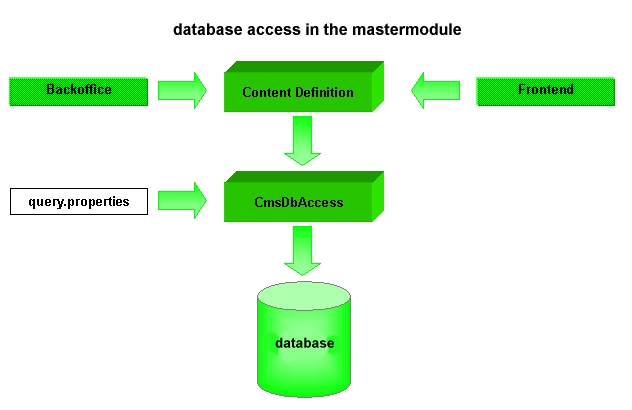
\includegraphics[clip,width=\sgw]{pics/modules/masterclasses}
\end{center}
\caption[database access in the mastermodule]
    {database access in the mastermodule}
\label{databasemaster}
\end{figure}

The method {\meth publishProject()} must be implemented to publish the module data. You can take
this example implementation and only have to replace the name of the Content Definition class:

\begin{verbatim}
public static void publishProject(CmsObject cms, Boolean enableHistory,
            Integer projectId, Integer versionId, Long publishingDate,
            Vector changedRessources, Vector changedModuleData) 
            throws CmsException {

        // publish the ressources for this module
        CmsMasterContent.publishProject(
            cms, 
            enableHistory.booleanValue(),
            projectId.intValue(), 
            versionId.intValue(),
            publishingDate.longValue(), 
            C_SUB_ID, 
            YourContentDefinition.class.getName(),
            changedRessources, 
            changedModuleData
        );
    }
\end{verbatim}

To make sure that this method gets called when the project is published you also have to 
provide the name of the Content Definition class in the {\name registry.xml} file of 
OpenCms inside the section for your module:

\begin{verbatim}
<modules>
  <module>
    <name>module.package</name>
      ...
      <publishclass>
        <name>module.package.YourContentDefinition</name>
      </publishclass>
      ...
   </module>
</modules>
\end{verbatim}

The method {\meth moduleParameterWasUpdated()} is used to read the module parameters from the 
OpenCms {\name registry.xml} file. The method is automatically invoked on the eventhandling class 
of the module (this should be your Content Definition class)
when the parameters are changed via the module administration of OpenCms. The mastermodule uses 
several parameters to provide the database urls for online, offline and backup tables and the type of the database:

\begin{verbatim}
/**
 * Reads the module parameters from the registry.
 * Automatically invoked when the parameters are changed
 * in the module administration.
 * @param cms - CmsObject to access system resources.
 */
 public static void moduleParameterWasUpdated(CmsObject cms) 
         throws CmsException {
     // read all poolnames from the module parameters
     String connect = OpenCms.getRegistry().getModuleParameterString(
         "module.package", "onlinePool", "jdbc:opencmspool:mysqlonline");
     String connectOffline = OpenCms.getRegistry().getModuleParameterString(
         "module.package", "offlinePool", "jdbc:opencmspool:mysql");
     String connectBackup = OpenCms.getRegistry().getModuleParameterString(
         "module.package", "backupPool", "jdbc:opencmspool:mysqlbackup");
     // read the dbtype from the module properties
     String dbType = OpenCms.getRegistry().getModuleParameterString(
         "module.package", "dbType", "genericsql");
     // read the root channel from the module properties
     String rootChannel = OpenCms.getRegistry().getModuleParameterString(
         "module.package", "rootChannel", "/");

     if("genericsql".equalsIgnoreCase(dbType)){
         CmsDbAccess dbAccess = 
		     new CmsDbAccess(connectOffline, connect, connectBackup);
         CmsMasterContent.registerDbAccessObject(C_SUB_ID, dbAccess);
         dbAccess.setRootChannel(rootChannel);
     } else {
         throw new CmsException("No database selected");
     }
}
\end{verbatim}

The method reads the parameters {\name onlinePool}, {\name offlinePool} and {\name backupPool}
that define the jdbc urls for access to the online, offline and backup tables of the module.
The third String parameter in the method call to {\meth getModuleParameterString()} is a default
value that will be returned by the method if the parameter is not specified in the {\name registry.xml} 
file. If you omit this parameter the method will return null if the parameter cannot be found.
The parameter {\name dbType} is used to control which database will be used. Depending on this
parameter the appropriate CmsDbAccess object will be created with the urls for the online, offline 
and backup tables. Another module parameter is the {\name rootChannel} parameter. It is used to
define a parent channel for all channels accessible for this module. For example if the root channel
is set to /news/ all subchannels of /news/ will be available in the backoffice to put a news entry
in it. This way you have a seperation of channels of different modules. The value of the {\name rootChannel}
must be set in the {\name CmsDbAccess} object. 
If you don't set it, it will be set to the default value, the root folder ("/"). So if you don't need channels
in your module you can simply forget about this parameter.
 
%%% Local Variables:
%%% mode: latex
%%% TeX-master: "OpenCmsDoc"
%%% End:

\chapter{Static Export}

\section{Introduction}

Since version 4.6 OpenCms has the feature "Static Export". With this feature it is possible to export the static resources to a docroot in the server filesystem. During this export all links to this static resources and back to dynamic resources will be adjusted automatically. In this scenario it is possible that a traditional web server like Apache (\rqhttp{http://httpd.apache.org}{http://httpd.apache.org}) serves all static resources and OpenCms delivers all dynamic resources (like forms or personalized sites). This splits up the work to each software that can handle the specific request in a better way.

\section{Setting up Static Export}

The static export is already preset for a tomcat standalone installation, so you don't have to modify anything if you use tomcat in standalone-mode and can jump to the next section.

In the file opencms.properties (located in \texttt{webapps/opencms/WEB-INF/config/}) you can enable static export:

\texttt{staticexport.enabled = true}

Note: If you enable the static export your publishing cycle will slow down because of the additional work of exporting the resources to the server filesystem.

After this you have to define the export path on your server. This path should be the http-servers docroot or a subdirectory of it. If you define a relative path it is relative to your webapplication.

\texttt{staticexport.path = export/}

Now you have to define some url\_prefixes so the static export can adjust all links to the correct location (http-server or OpenCms).

\begin{verbatim}
url_prefix_export = /${WEB_APP_NAME}/export
url_prefix_http   = /${WEB_APP_NAME}/opencms
\end{verbatim}

The string \texttt{\${WEB\_APP\_NAME}} will be replaced by the current name of the webapplication. In normal installations this would be opencms.

Now you can define resource(s) the static export should start with. This can be a single or multiple file(s) or folder(s). This property is only used if you start the static export manually (via admin view).

\texttt{staticexport.start = /}

All the other properties for static export are advanced properties. In normal installations you will never need to adjust them on your own. If you are interested in them you should have a look into the comments of the opencms.properties file.

\section{How to use static export}

To get used to the static export you should create two pages like \texttt{/index.html} and \texttt{/page1.html}. You should add some content to this pages and create a link from each page to the other with the HTML edit control. Now you can publish your project. If static export is enabled all changed resources will be exported to the server filesystem into the folder you have specified. The two links will be adjusted, so they will refer to each other even after the export. You can browse the two resources by pointing your explorer or navigator to the following location:

\texttt{http://yourserver.com:8080/opencms/export/index.html}

This is the static copy of the resource you can reach with:

\texttt{http://yourserver.com:8080/opencms/opencms/index.html}

\section{What have I to do?}

OpenCms needs your help to adjust all links between resources. Therefore you have to mark all links in the templates (mastertemplates, frametemplates, contenttemplates and elements) with the tag \texttt{<link>}. In this link tag you define the link to another resource within the OpenCms system (No scheme, server name, port or webapplication name is allowed). You can add url parameters to the link, if you need:

\begin{quote}
\begin{verbatim}
href="]]><link>/index.html</link><![CDATA["
href="]]><link>/news.html?newsid=7</link><![CDATA["
src="]]><link>/pics/logo.gif</link><![CDATA["
\end{verbatim}
\end{quote}

An editor can use the HTML edit control. OpenCms will take care about links added with the control. Therefore it uses the JTidy library to find all "a href" and "img src" tags and inserts the needed OpenCms link tag.

A module developer has to call the method getLinkSubstitution to get adjusted links:

\texttt{String adjustedLink = cms.getLinkSubstitution(String link);}

You need to call this method for dynamic creation of pages. E.g. a navigation element that creates a list of links dynamically should call \texttt{getLinkSubstitution} for each navigation entry.

\section{How does static export work?}

After the publishing to the online project is done OpenCms starts to export all static resources. It starts with all changed resource(s) in that project. After the export of this resource(s) it will follow all links defined in the link tags or substituted with the \texttt{getLinkSubstitution } method. These resources will be exported, too. This cycle will end if all resources are exported.

A next run of the static export will only export the changed resources. A resource is marked as changed, if one of the resources this resource depends on was changed. OpenCms will find the "normal" dependencies like mastertemplate, frametemplate, contenttemplate and elements. Additional dependencies like dependencies for dynamic navigation templates or displaying content definitions you have to register yourself. How to register these dependencies you have learned in the chapter about using the element cache.

Note: You can find the names of all exported resources in the opencms.log file. So you can check which resources are exported.

\section{How to control what is exported?}

Only resources that are readable as a \texttt{Guest} user are exported. You can control the export behaviour of these resources by adding properties to that resource. The property "\texttt{export}" controls if and how the resource will be exported. The following values are possible:

\begin{itemize}
\item false:\\
The resource will never be touched by the export (not exported and no link adjustment)

\item dynamic:\\
The resource is dynamic. It will not be exported. All requests will be delivered by OpenCms. A link to this resource will be adjusted to a link into the OpenCms system.

\item https:\\
The resource is dynamic. A link to this resource will be adjusted to a link into the OpenCms system. Additionally the scheme will be set to https. You need to configure OpenCms and the web server to handle https requests.

\item true, or no property:\\
This is a static resource. The resource will be exported to the docroot of the web server.

\item https\_enabled:\\
This is a static resource. The resource will be exported to the docroot of the web server. The links to this resource from a https page will not be set to http. Used to show pics on a https page.

\item dynamic\_https\_enabled:\\
Like dynamic but the links to this resource from a https page will not be set to http. 
\end{itemize}

You can control the name of an exported resource with the property "\texttt{exportname}". This is useful for modules which reside in the folder 

\texttt{/system/modules/YOURMODULENAME/YOURMODULEFILES}. 

If you want to reach the resource with a shorter and nicer URL you can define the "\texttt{exportname}" property. You should add it to the folder \texttt{YOURMODULENAME} and set it to a nice short path (e.g. \texttt{/YOURSHORTMODULENAME/}). After the export was done, you can reach your module with the URL:

\texttt{/opencms/export/YOURSHORTMODULENAME/YOURMODULEFILES}

instead of

\texttt{/opencms/export/system/modules/YOURMODULENAME/YOURMODULEFILES}.

Note: You can control single resources or complete folders with all sub resources by adding the property "\texttt{export}" and "\texttt{exportname}".

\section{How to export resources with parameters?}

OpenCms will even export static resource with parameters:

\begin{quote}
\begin{verbatim}
/news.html?newsid=7&channelid=25 -> /news_1.html
/news.html?newsid=44&channelid=3 -> /news_2.html
...
\end{verbatim}
\end{quote}

The parameters will be substituted to a consecutive number. There is no relationship between the consecutive number and the URL parameters.

\section{Advanced properties of the static export: switch standard to dynamic}

As above mentioned there are properties for the static export you may wish to use as a advanced user. 

The static export is controlled by the resource property export. Normaly a resource with no property set (including the parent folders) is handeld as if the property is set to true. This feature is good when most of the side is static and can be exported, but when everthing is dynamic you sure want OpenCms to export only files with the property export=true and let everything withouth the export proptery stay in OpenCms. Therefore you can set the default value for the export property to 'dynamic'.

\texttt{staticexport.default.export=dynamic}

Only 'true'(standard) and 'dynamic' are allowed. There are two set of linkrules defined in the opencms.properties. In the dynamic mode the second ruleset is used. This ruleset includes automatical export of some filetypes like css, js, gif, jpg,... If you want additional filetypes automaticaly exported, just add the corresponding lines to the ruleset.dynamic\_exportrules and the ruleset.dynamic\_externrules:

\begin{quote}
\begin{verbatim}
s#(.*\.ppt$)#${url_prefix_export}$1#,\
s#(.*\.ppt$)#$1#,\
\end{verbatim}
\end{quote}

Note that all files will be exported that include the '.ppt' at the end of there name.

\section{Advanced properties of the static export: Configure Https}

If you want to use the ssl protocol you can configure the static export to set the scheme as prefix ahead of the link if the Page has the https property and to set the http scheme ahead of links that reference from a https page to a http page. 
All this is done automaticaly by OpenCms. You just have to set the property "export" to https on the folder where your ssl pages are. Then you configure the prefixes in the opencms.properties:

\begin{quote}
\begin{verbatim}
url_prefix_https=https://server.de/${WEB_APP_NAME}/opencms
url_prefix_servername=http://server.de
\end{verbatim}
\end{quote}

The servername is used in addition to the export resp. the http prefix for links from https to http pages. The https prefix is set ahead of links to the https pages. Note that only link tags will be processed. If you write a template, don't forget to use it consequently.

\section{Advanced properties of the static export: Relative Links in Export}

If you just need a static site with no dynamic content you might want to use the exported pages without OpenCms. Then it could be necessary to have all links in the export relative. 

\begin{quote}
\begin{verbatim}
relativelinks_in_export=true
\end{verbatim}
\end{quote}

This feature only works with the standard rulesets and it needs some extra performance.

\section{Advanced properties of the static export: The Rulesets}

In the majority of cases you don't need to modify the linkrules. 
First you can configure which ruleset is used for which situation. OpenCms needs four rulesets. Three for the link replacement for a link on a page that is a) shown in the online project, b) shown in the offline project and c) exported to the filesystem. The fourth rule is used for OpenCms to know under which name a exported page should be saved in the filesystem. Mostly the export and the online rules are the same. 

\begin{quote}
\begin{verbatim}
linkrules.true.export=exportrules
linkrules.true.online=exportrules
linkrules.true.offline=offlinerules
linkrules.true.extern=externrules
linkrules.dynamic.export=dynamic_exportrules
linkrules.dynamic.online=dynamic_exportrules
linkrules.dynamic.offline=dynamic_offlinerules
linkrules.dynamic.extern=dynamic_externrules
\end{verbatim}
\end{quote}

Which definition is used depends on the value of the staticexport.default.export parameter: true or dynamic. The value of the linkrules must apear as the name of a ruleset in the opencms.properties. 

A ruleset is a commaseperated list of substitution rules in perl5 standard. 
In General when a link tag is resolved or the getLinkSubstitution() method is called in a module one rule after the other is executed till a rule matches. Then the result is returned. When it comes the the *dynamic rules* entry the dynamic rules OpenCms has generated with the resource property 'export'. In this case all dynamic rules are executed till one matches. If nothing matches the original is returned. 
You can use the \$\{WEB\_APP\_NAME\} variable for the webapplication name and the
four prefix variables defined above (\$\{url\_prefix\_export\}, \$\{url\_prefix\_http\},...).
They will be replaced befor using the regular expression.
In addition to this it is possible to define the place where the dynamic
generated rules should be used instead of a rule use the expression 
*dynamicRules* (including the *'s). OpenCms replaces this with the dynamic
generated rules.
There are two types of dynamic rules. The first one is generated with the 
resourceproperty "exportname". For each resouce with this property a rule 
will be generated that replaces the absolute path of this resource with the 
value of the property. It is principally used to get nice short foldernames 
on the disc.
The second kind of dynamic rules are generated with the property "export".
The value can be 'dynamic' or 'https'. The system generates
rules so that the links to these resources go back to the opencmssystem from the 
static content (with protocol https in the second case).
There is a third value posible: 'false' means the resource is not exported and it 
will not be created for getting furter links on it like the 'dynamic' ones. 
New possible values are 'true', 'https\_enabled' and 'dynamic\_https\_enabled'. True 
is needed for the case when default is set to dynamic. https\_enabled works like true
but it will not set the http scheme ahead the link. dynamic\_https\_enabled is the same 
for dynamic resources.

The dynamic rules are only for export, online and extern rules. Don't use them in 
the offlineruleset.
The parameterreplacement is done in the dynamic rules. So it works together with
the exportname rule. If you have a rule befor the dynamic rules that is triggered
the parameterreplacement will not happen.

%==========================================================
% The OpenCms synchronization
%==========================================================
\chapter{The OpenCms synchronization}
\label{synchronization}

\section{What is synchronized?}
%============================================================================
The synchronization tool \index{synchronization} is used to synchronize \index{synchronize} files in the Virtual File System \index{Virtual File System} of OpenCms and their corresponding files in the Server File System \index{Server File System}.

It's a feature for development only. It speeds up the development cycle because you can modify the file on your Server File System with your favorite application and update the file in the filesystem of OpenCms.

\index{synchronizationmanagement}
\section{Manage the properties for OpenCms synchronization}
%============================================================================
The synchronization requires some entries in the {\dir
registry.xml}. You will find the registry in your configuration
path of OpenCms ({\dir config/}). You need to enable and modify
the following section:

\begin{xml}
<syncpath>c:/work41/sync</syncpath>\\
<syncproject>\_syncProject</syncproject>\\
<syncresource>\\
\xtaba  <res1>/content/</res1>\\
\xtaba  <res2>/download/</res2>\\
\xtaba  <res3>/pics/</res3>\\
</syncresource>\\
\end{xml}

The {\tag <syncpath>} \index{syncpath} is the path on your server
where you want to save the synchronized files. The {\tag
<syncproject>} \index{syncproject} is the name of your project in
OpenCms whose files you want to synchronize. In the section {\tag
<syncresource>} \index{syncresource} you put the names of the
resources you want to be synchronized. Put each resourcename
between a tag named {\tag <resx></resx>} where the {\name x} is a
serial number.

To make it easier for you to manage these entries there is a
management tool in the backoffice. Only administrators are allowed
to manage the synchronization properties.

\begin{figure}[hbt]

\begin{minipage}[b]{0.499\linewidth}
  \begin{center}
  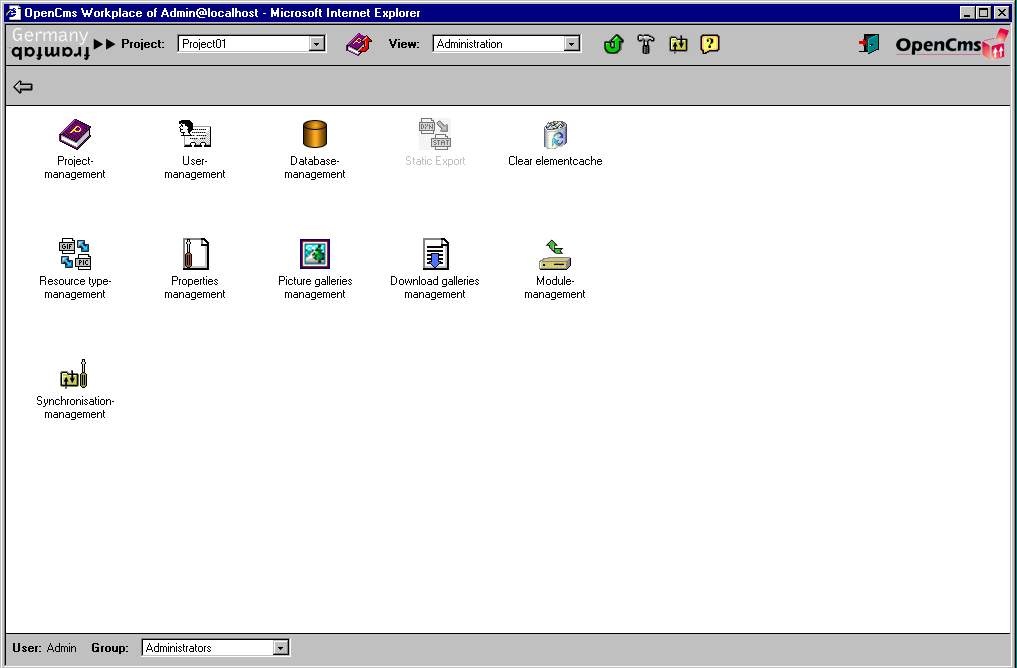
\includegraphics[clip,width=\sgw]
                   {pics/synchronize/syncprop01}
 \end{center}
\end{minipage}
\hfill
\begin{minipage}[b]{0.499\linewidth}
   \begin{center}
   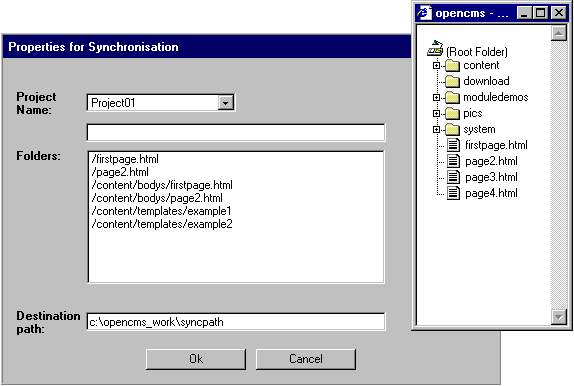
\includegraphics[clip,width=\sgw]
                   {pics/synchronize/syncprop02}
   \end{center}
\end{minipage}
\caption[The synchronization management icon and dialog]
           {The synchronization management icon and dialog}
 \label{syncproperties}

\end{figure}

A click on the icon will open the dialog for synchronization
management. If the entries for synchronization already exist in
the {\dir registry.xml}, they will be shown in the dialog.

You can choose any project from the project list. The list
contains your accessible projects accept the online project. So
there must be at least one offline project. When you have chosen a
project the folder tree, that you get with the folder button,
shows the resources in this project. By clicking on a resource you
can add it to the resource list for synchronization. You can also
add resources by fill in the resource name into the field above
the resource list and clicking the arrow button. To remove
resources from the list you use the delete button.

The third entry that is needed is the destination path on your
server.

When you choose all entries you can update the registry by
clicking on 'OK'. There will be errormessages if you left the
project, the resource list or the destination path empty or if a
resource can not be read from the choosen project.

\section{How to synchronize}
%============================================================================

If there are the required entries in the registry.xml the button
for synchronization will appear in the head section between the
icons for the preferences and the help (Figure~\ref{syncicon}).

\begin{figure}[hbt]
\begin{center}
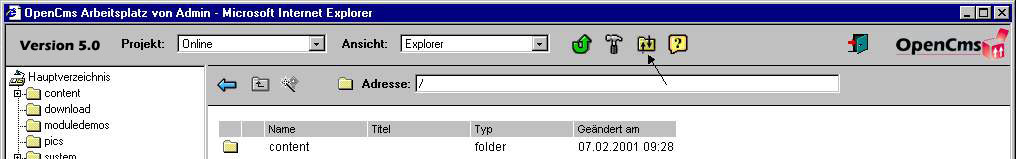
\includegraphics[width=\sgw]
                   {pics/synchronize/syncico}
\caption[The button for synchronization]
           {The button for synchronization}
\label{syncicon}
\end{center}
\end{figure}

A click on the button will start the synchronization. If the project for synchronization, which you specified in the registry, does not exist it will be created and the resources that should be synchronized will be copied from the online project to the synchronization project.

The synchronization will not work if there is more than one project with the name of the synchronization project or if the resource to be synchronized does not exist in the project.

\section{How the files are synchronized}
%============================================================================
First the resource and all its subresources are read from the Virtual File System and checked for changes.

\begin{itemize}
\item The resources that does not exist on the Server File System will be created.
\item If the resource is marked as deleted the corresponding resource will be deleted from the Server File System.
\item Files are compared with the entries in the {\dir synchronize.list}.
\end{itemize}

The {\dir synchronize.list} is created after the synchronization and contains the name of each synchronized file and the date of its last modification in the Virtual File System and the Server File System.

\begin{itemize}
\item If the date of the last modification of the file on the Virtual File System is after the corresponding date in the {\dir synchronize.list} the modification date of the file on the server is checked.
    \begin{itemize}
    \item If the date of the file on the server has not changed after the last synchronization, the file will be updated with the content of the file on the Virtual File System.
    \item Has the file be changed on the Server File System, too, it will be copied to a backupfile (the backupfile is marked with a leading {\name \$}) and updated with the content of the file on the Virtual File System.
    \end{itemize}
\item If the file has not be changed on the Virtual File System but on the Server File System, the file on the Virtual File System will be updated with the content of the file on the Server File System.
\end{itemize}

After the resources on the Virtual File System were checked, the filelist of the resource on the Server File System is read. The Virtual File System is checked if it contains all of the files and folders in this list. Files and folders that does not exist in the Virtual File System are created.

%%% Local Variables:
%%% mode: latex
%%% TeX-master: "OpenCmsDoc"
%%% End:

%============================================================================
\chapter{System architecture}
%============================================================================

\section{Components}
%============================================================================
OpenCms is a client server application that can be used in HTTP-based
environments such as the Internet. OpenCms is a classic web application
with a 3-tier-architecture (figure~\ref {3-tier1}).

\begin{figure}
\begin{center}
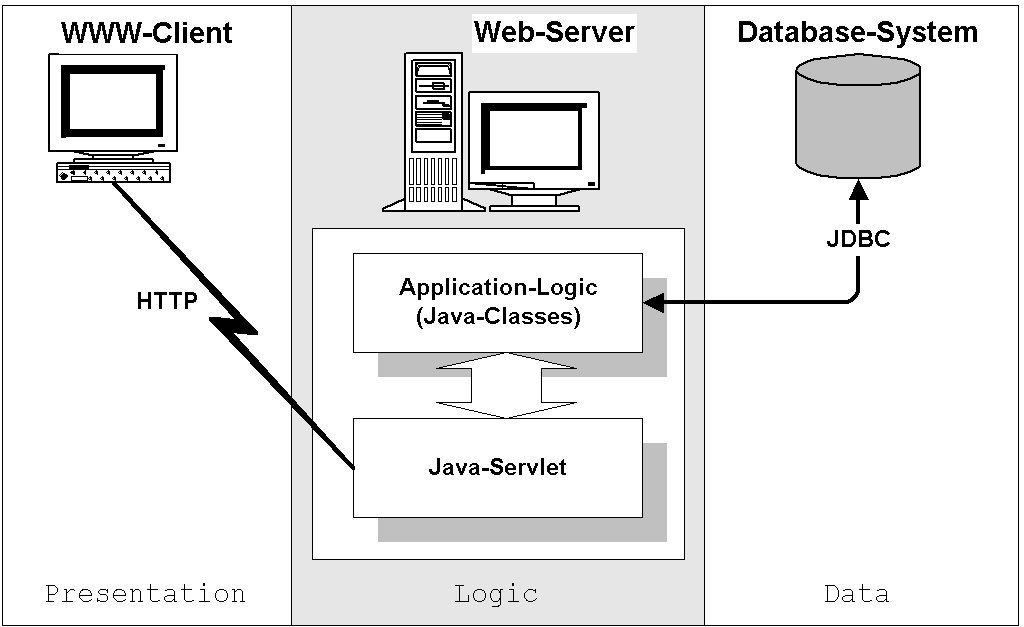
\includegraphics[clip,width=\sgw]{pics/modules/1}
\end{center}
\caption[3-tier-achitecture]{Example of a 3-tier-architecture using OpenCms}
\label{3-tier1}
\end{figure}

The presentation layer consists of a web browser (Internet Explorer or
Netscape Navigator) that is used to display and navigate through the HTML
user interface. Regardless of the browser used, it must be Version 4 or
higher. If you use an older version of the browser you will not be able
to execute the existing DHTML functions (JavaScript code) or attach
external style sheets. Both are necessary for a correct  usage of the
application.

The logic layer lies on the web server, which is extended by a runtime
environment for Java servlets. The web server can be the Apache web
server (Version 1.3.6 or higher), the configuration of which must be
completed by the so called "Jserv module" (the Servlet Engine,
Version 1.0 or higher), in order to execute servlets. All Java classes
are installed in the servlet environment on the server.
The OpenCms servlet (one single class) provides the interface to the
presentation layer as well as the interface to the database layer. It
uses the HTTP protocol to establish the communication between the
client and the application on the server (in this case OpenCms).
The database is accessed through the JDBC interface. The database
contains tables for resource, user and property data.

The following figure shows the most important components of OpenCms 
(Figure~\ref {Components}).\\

\begin{figure}
\begin{center}
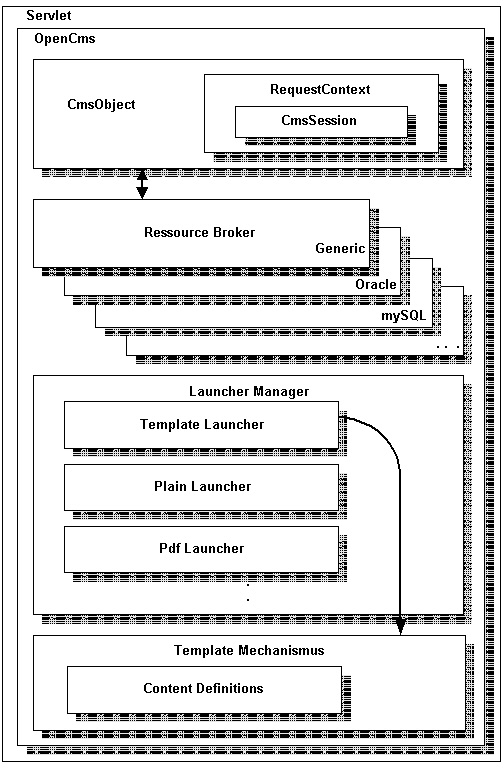
\includegraphics[clip,width=0.7 \linewidth]{pics/modules/2}
\end{center}
\caption[Components]{Compoments}
\label{Components}
\end{figure}


{\bf CmsObject:}
All resources are accessed via the \index{CmsObject} CmsObject. This is the interface to
the OpenCms system for the Module Developer. The CmsObject is
initialized with the user data.

{\bf Resource Broker:}
The \index{resource broker} resource broker checks requests for resources and performs them if
the user has the appropriate access permissions. It's configuration
depends on the database that is used.

{\bf Launcher Manager:}
The \index{Launcher Manager} Launcher Manager determines the launcher that will generate the
output with the requested content based on the type and/or content of
the selected file. If the template launcher has been selected, the
Template Mechanism is started.

{\bf Template Mechanism:}
The \index{Template Mechanism} Template Mechanism creates HTML pages based on the content in its
structured form. Content definitions enable you to access content that
originates from different sources (e.g. Virtual File System (VFS),
database, file system ...).


\section{Accessing system resources}
%============================================================================
The general procedure of requesting an OpenCms web page is shown in the
next figure. First, a request is sent from the web browser. The URL
contains the host, the servlet path and the URI. The web server starts
the \index{servlet engine} servlet engine because the URI is within the servlet path, enabling
the servlet engine to pass it to OpenCms (Figure~\ref {Accessing1}).

\begin{figure}
\includegraphics[clip,width=\sgw]{pics/modules/3}
\caption[Accessing system resources]{Accessing system resources}
\label{Accessing1}
\end{figure}

System resources are accessed via an instance of the class {\name CmsObject},
which provides the public interface that is used to access the system
and create the corresponding context. From the {\name msObject}, requests are
forwarded to the non-public parts of OpenCms. Thus, an instance of the
class {\name CmsObject} is created and initialized with the current user first.
The{\name CmsObject} passes the resource request to the resource broker. The
{\name resource broker} is the interface to the database. It performs the
request via the database access module and returns the resource if the
user has the right to access it. The access module establishes the
connection between the logic layer (application) and the database layer.
If a resource is requested, the {\name resource broker} forwards the request to
the access module. The access module generates an SQL statement to get
the data from the database. It then generates a {\name CmsRessourcObject} from
the database data and returns it to the resource broker. The {\name resource
broker} can now check the access permissions of the file and return the
file to the {\name CmsObject} providing the user has the appropriate access
permissions.

Because OpenCms works with different kinds of databases, the {\name resource
broker} and the access module are configured according to the used
database (Oracle, mySQL, etc.).
\index{database}
The following figure shows the structure used to access resources (figure~\ref {Accessing2}).

\begin{figure}
\begin{center}
\includegraphics[clip,width=\sgw]{pics/modules/4}
\end{center}
\caption[Accessing resources in OpenCms]{Accessing resources in OpenCms}
\label{Accessing2}
\end{figure}

If the operation is successful (i.e. the user has permission to read
the file), the resource is displayed (sent to the user's web browser).

This is done by the {\name Launcher Manager}. The {\name Launcher Manager} starts a
certain launcher according to the type of the requested resource. For
pure text files, images etc. the plain launcher is used, which forwards
the content of the resource directly. The {\name template launcher} is used to
start the Template Mechanism when a template is requested. The {\name Template
Mechanism} creates HTML pages based on the content in its structured form.

The different launchers and the {\name Template Mechanism} will be explained in
detail in the following chapters.
\newpage

\section{Resources}
%============================================================================
All of the Objects that are administrated in OpenCms are called
{\name resources}. At the moment, there are eight different types of
resources. With the exception of the resource type {\name folder,} all other
types are resources files that have content that can be displayed in a
browser. The  resource type is used to provide every file with aresources
processing instance - called {\name Launcher} - which starts the processing
process and then displays the data. The following table shows the
existing relationships. {Table~\ref {resources}}
\index{resource type}
\begin{table}[h]
\begin{center}
\begin{tabular}{|l|c|p{0.50\linewidth}|l|}
\hline
{\bf Name}& 
{\bf ID}& 
{\bf Description}& 
{\bf Launcher}\\ \hline
folder&
0& Folder&none\\ \hline
plain&
1&
Files that are notprocessed by OpenCms (text files, JavaScript libraries etc.)&
Dump launcher\\ \hline
XMLTemplate&
2&
XML coded template file.&
XML launcher\\ \hline
page&
3&
Representation of a whole site ("clickable file" or "page file").&
XML launcher\\ \hline
binary&
4& 
Binary files (like zip archives and PDF documents, but not graphics) that can be uploaded.&
Dump launcher\\ \hline
image& 
5& 
Binary graphic files (like  GIFJPEG& 
Dump launcher\\ \hline
script& 
6& 
Designed for JavaScript on the server- side& 
Dump launcher\\ \hline
newspage&
7& 
Representation of a news article, special caseof a page file& 
XML launcher\\ \hline 
\end{tabular}
\caption [Resources in OpenCms]{Resources in OpenCms}
\end{center}
\label{resources}
\end{table}

\section{The Virtual File System (VFS) of OpenCms}
\index{Virtual File System}
\index{VFS}
All of the files and folders of the different projects that are
displayed in the Explorer view that is part of the OpenCms Workplace,
are not stored in the normal file system. OpenCms has a {\name Virtual File
System} that holds the files and folders in a database, and an integrated
access permission administration. The access permissions in OpenCms are
similar to those of the UNIX file system. However, by using a {\name VFS} and a
database, OpenCms is independent from the operating system that is
installed on the server. In this way OpenCms can run on a Windows 95/98
system, which itself has no access permission administration at all.
Here is a short overview of the folders and the files in the standard
OpenCms {\name Virtual File System:} {Table~\ref {VFS}}

\begin{table}
\begin{center}
\begin{tabular}{|l|p{0.55\linewidth}|}
\hline
{\bf Directory}&
{\bf Files located in the directory}\\ [0.5ex] \hline
{\dir /content}&
Parent directory of  the directories that store the template files.\\ \hline
{\dir /content/bodys}&
Body templates are stored in this directory or a subdirectory thereof. They are stored in a directory with the same name
as the directory in which the web site is located.\\ \hline
{\dir /content/internal}&
Templates (subtemplates) that are not body  or master templates.\\ \hline
{\dir /content/templates}&
The master templates that define the general layout of a web site.\\ \hline
{\dir /download}&
Subdirectories for files that can be downloaded (galleries).\\ \hline
{\dir /pics}&
Subdirectories for pictures that are used in web sites (galleries).\\ \hline
{\dir /system}&
Parent directory of the directories that contain workplace templates and configuration files for the system.\\ \hline
{\dir /system/workplace/action}&
Executable files like login, copy etc.\\ \hline
{\dir /system/workplace/administration}&
Subdirectories for every Item in the Administration view.\\ \hline
{\dir /system/workplace/config}&
The language files, that are stored in a separate subdirectory for every language, and  the different
configuration files.\\ \hline
{\dir /system/workplace/css}&
Used style sheets.\\ \hline
{\dir /system/workplace/help}&
The help system.\\ \hline
{\dir /system/workplace/pics}&
The pictures that are used to create the workplace.\\ \hline
{\dir /system/workplace/templates}&
The templates that are used to create the workplace.\\ \hline
\end{tabular}
\caption [VFS of OpenCms]{VFS of OpenCms}
\label{VFS}
\end{center}
\end{table}

\section{Class structure}
%============================================================================
The functionality of OpenCms is implemented in many different Java
classes. The classes are divided into different packages to structure
the code. Currently, there are 10packages that  cover a certain part
of the system's functionality.{Table~\ref {Classtruc}}

\begin{table}[h]
\begin{center}
\begin{tabular}{|l|p{0.55\linewidth}|}
\hline
{\name com.opencms.core}&
Classes of the system's core. The package also contains the OpenCms servlet.\\ \hline
{\name com.opencms.file}&
Definitions of all of the objects. \\ \hline
{\name com.opencms.file.genericSql}&
Resource broker for generic SQL databases. \\ \hline
{\name com.opencms.file.mySql}&
Special resource broker for mySQL.\\ \hline
{\name  com.opencms.file.oracleplsql}&
Special resource broker for ORACLE.\\ \hline
{\name com.opencms.file.utils}&
File package.\\ \hline
{\name com.opencms.launcher}&
All of the launchers that are used to display files or templates and a Launcher Manager.\\ \hline
{\name com.opencms.template}&
All of the template classes that are used to create documents dynamically and a Template Manager.\\ \hline
{\name com.opencms.util}&
Some general functionality (encoder, decoder etc.)\\ \hline
{\name com.opencms.workplace}&
All of the components (e.g. buttons, context-sensitive menus etc.) and functions (e.g. create project) of
the user interface (OpenCms Workplace).\\ \hline

\end{tabular}
\caption [Class structure]{Class structure}
\label {Classtruc}
\end{center}
\end{table}
\chapter{Core Development}

\section{Introduction}

In this section you can learn something about the interna of OpenCms. This
is interesting for people who want to contribute to the project at 
core\-level. Currently there are two subsections. One about how to build
OpenCms from scratch by your own using ant. The other about interna of the
project mechanism used by OpenCms since version 4.4.

\section{How to compile the OpenCms core}
OpenCms provides a full source distribution that you can use to build the
OpenCms core. This is only needed if you want to add your own core 
extensions. To develop the usual kind of website functionality, you 
should use the OpenCms module mechanism which is much easier to start with 
and also much better documented. Before even considering starting to work 
on the core, you definitly should have written some OpenCms modules to 
understand the separation between a module and a core extension. 

The OpenCms core comes with the best possible documentation: The source
code itself. This is really not something for the novice Java developer.
However, if you have some experience in Java, Java Servlets, JDBC, XML in 
general and the Apache Xerces API you might take a look. As said before, 
you should also have already a firm understanding of the OpenCms module API. 

Since this is rather deep stuff more for experts than for beginners, I 
will not explain every detail of the process.

\subsection{Before you start}

In case you really intend to contribute to the OpenCms core development, 
please make sure you use the latest version from the CVS source tree. The
source distribution ZIP file provided for download is the code of the latest
major release, not the current development status of OpenCms. The ZIP provides
a good starting point, but contributions should be based on the latest 
development version. The way to do it is to first get the source distribution 
(because it also contains the libaries), see if you can build this, and then 
simply checkout the latest \texttt{/opencms} directory from the CVS, replacing the 
\texttt{/opencms} directory from the source distribution (see below).

Ok, now on to the real work:

\subsection{Have Ant installed}

Apache Ant is a Java based build tool. In theory it is kind of like make
without make's wrinkles. You need Ant version 1.4 or later to build the 
OpenCms core. Ant is part of the Jakarta Apache Project 
(\rqhttp{http://jakarta.apache.org/}{http://jakarta.apache.org/}) and can be downloaded
here: \rqhttp{http://jakarta.apache.org/ant/}{http://jakarta.apache.org/ant/}. 
Please check the Ant documentation to make sure you understand the basic 
principles behind Ant. 

Ant installation is described in the manual
(\rqhttp{http://jakarta.apache.org/ant/manual/}{http://jakarta.apache.org/ant/manual/}). 
It requires that you have set up your path to Java correctly. Make sure 
Ant runs before proceeding.

\subsection{Get the OpenCms Source distribution}

Download the latest OpenCms source distribution. It contains all classes 
neccessary to build the OpenCms core. You can also checkout an OpenCms version
from our CVS tree, but make sure you have downloaded the source distribution 
before that because the necessary libraries are not included in the CVS. 

The source distribution comes in a ZIP file. Unpack this in your working 
directory, lets say this is called \texttt{/work}. You will then end up with the 
following structure in your work directory:

\begin{verbatim}
/work
    /opencms               <= Start of the OpenCms source tree
        /etc
        /src
        /web
        build.xml          <= This is needed by Ant 
        ...  
    /ExternalComponents    <= Contains the neccessary libaries
        activation.jar
        fesi.jar
        ...
\end{verbatim}


\subsection{Get additional classes (optional)}

In case you want to use the Oracle database, you need the Oracle JDBC driver
which you can download from the Oracle Technology Network 
(\rqhttp{http://otn.oracle.com}{http://otn.oracle.com}). You have to register 
there to get the driver. The file 
you need is the JDBC driver called classes12.zip. Place the file in the 
directory \texttt{/ExternalComponents} of the OpenCms source tree (see above). If you 
don't have this file, the OpenCms Oracle Driver 
(package org.opencms.file.oracleplsql) is not compiled, which is ok if you 
don't run on Oracle.

\subsection{Build the source by starting Ant}

Ok this is the easy part. Call up a commandline, move to the \texttt{/opencms} 
directory (where the file \texttt{build.xml} resides) of the OpenCms source tree. 
In your commandline, enter the following: 

\texttt{ant all} 

That's it! This will build a complete OpenCms distribution. Your work 
directory will look like this after Ant is finished: 

\begin{verbatim}
/work
    /opencms               <= Unchanged
    /ExternalComponents    <= Unchanged
    /build
        /classes           <= Will contain the compiled OpenCms classes
        /opencms           <= This is the standard .war directory layout
            /WEB-INF
                /lib
                /oclib
            /META-INF
    /zip                   <= The OpenCms distribution file will be placed
    /pdf                      here
\end{verbatim}


The final result of the compilation will be a ZIP file which will be placed 
in the \texttt{/zip} directory. This ZIP is exactly the same layout as the OpenCms
binary distributions, so it will contain the opencms.war archive. 

\subsection{Install your new version}

Now that you have your new OpenCms binary distribution, you simply need to 
follow the installation guide for your server setup. Please make sure you 
don't mess up any existing installation. Best have a separate machine that 
is used only for testing and development. 

\subsection{Other Ant targets}

There are several more targets in the ANT that might be useful for you.
Here's a short overview:

\begin{itemize}
\item Ant target: \texttt{war}\\
This creates the opencms.war, but does not create the binary distribution 
ZIP file.

\item Ant target: \texttt{srcdist}\\
This generates the source distribution ZIP file. Like the one you 
can download. 

\item Ant target: \texttt{tomcat.dist}\\
This is useful if you really are in developing core extensions. Provided
that OpenCms runs on your machine using Tomcat (and that you have all 
environment variables set up, esp. TOMCAT\_HOME or CATALINA\_HOME), calling 
this target will have Ant updating the OpenCms classes on your machine. 
This is done by replacing the files in the Tomcat \texttt{webapps/opencms} directory.
If you have renamed opencms.war, or if your Tomcat is not installed the 
usual way, this probably will not work.

\item Ant target: \texttt{setup}\\
This is an extension to tomcat.dist: It depends on tomcat.dist, but will 
also update the OpenCms database, provided you run MySQL on your development
machine. This is usefull if you do changes to the OpenCms Workplace template
files. CAUTION: This drops your complete database without further notice. 
Don't use until you know what you do. 

\item Ant target: \texttt{tex}\\
This generates the OpenCms documentation from the TeX sources. It's outside 
the scope of this document to explain what setup you need to do that.

\end{itemize}

To get a complete actual list of all targets please call ant with this parameter:\\
\texttt{ant -projecthelp}.

\subsection{Important}

In case you replace files in the Tomcat OpenCms \texttt{webapps} directory without doing a new setup of the database, you will get a message on login saying something like: 

\texttt{The version of workplace-templates and workplace-classes are different.\\Please update one.}

Since the workplace templates make very close usage of the core, this should 
definitely be fixed on production systems. To remove the message, make a new 
setup of the OpenCms database using the installation wizard from your newly 
generated binary distribution file. If you know what you do, you can ignore 
this message on development machines. 

\section{The Projectmechanism}
\index{Projectmechanism}

OpenCms contains a projectmechanism where all resources exist at least twice -
once for the "Online" project and once for all offline projects. If you 
have enabled versioning, the historic versions of the resources are also 
saved in a separate backup table space.

The projects that can be created with the project management are views on a shared set of offline resources.
If a resource is published, it is copied from the offline space to the online space
and from the online space to the backup (history) space.

\subsection{Data structure}
\index{resources data structure} \index{resources online}
\index{resources offline} \index{resources backup}

There are several tables for the online resources, the offline
resources and the backup resources. This minimizes the quantity of
data in the tables and accelerates queries on the data. Another
advantage is the possiblity to store online, offline and backup
resources on several databases. Each of these three groups has its
own database connection pool.

For the online resources there are the tables
\begin{itemize}
\item CMS\_ONLINE\_RESOURCES
\item CMS\_ONLINE\_FILES
\item CMS\_ONLINE\_PROPERTIES
\item CMS\_ONLINE\_PROPERTYDEF
\end{itemize}

The tables of the online resources are
\begin{itemize}
\item CMS\_RESOURCES
\item CMS\_FILES
\item CMS\_PROPERTIES
\item CMS\_PROPERTYDEF
\end{itemize}

The backup resources are stored in the tables
\begin{itemize}
\item CMS\_BACKUP\_RESOURCES
\item CMS\_BACKUP\_FILES
\item CMS\_BACKUP\_PROPERTIES
\item CMS\_BACKUP\_PROPERTYDEF
\end{itemize}
Each version of a backup resource has a version number. The
information of the project that was published is stored in the
backup tables

\begin{itemize}
\item CMS\_BACKUP\_PROJECT
\item CMS\_BACKUP\_PROJECTRESOURCES.
\end{itemize}

There is another new table named CMS\_PROJECTRESOURCES. This table
contains the ID of a project and the names of the resources that
were selected when the project was created. The entries describe
the view of the project on the offline resources.

\subsection{During installation of OpenCms}

When you setup OpenCms the first time to install the workplace
some data is filled in by default. With regard to the new
projectmechanism

\begin{itemize}
\item the online project is created as permanent project
\item the root folder is created in the online tables
\item the name of the root folder is inserted into the table CMS\_PROJECTRESOURCES for the online project
\item the setup project for the import of the workplace is created as temporary project
\item the root folder is created in the offline tables
\item the name of the root folder is inserted into the table CMS\_PROJECTRESOURCES for the setup project
\end{itemize}

Because the setup project is created by default the setupscript
does not create a project for the import of the workplace.

When the setup project is published the workplace will be copied
to the online tables and to the backup tables. The temporary setup
project will be deleted but the resources still exist in the
offline tables and can be accessed by creating a new project.

\subsection{Creating a new project}
\index{Project permanent}
\index{Project temporary}

A project can be created for permanent or temporary use. A
temporary project will be deleted after it was published.

\begin{figure}[hbt]
\begin{center}
\includegraphics[width=\sgw]
                   {pics/newProject/newPro01}
\caption[Creating a new project]
           {Creating a new project}
\label{newproject}
\end{center}
\end{figure}

When creating a new project only the names of the selected
resources are stored in the new table CMS\_PROJECTRESOURCES and no
resources are copied. So creating a new project is much faster
than before. The new project contains the selected resources and
always the folders \texttt{/system/galleries/pics/}, \texttt{/system/galleries/download/}, \texttt{/system/galleries/externallinks/}, 
\texttt{/system/galleries/htmlgalleries/} and  the folders
in \texttt{/system/bodies/} that correspond with the selected folders.

The project is now a view on the offline resources. If two
projects reference the same resource the changes on this resource
will be visible to both projects. If a folder is referenced in
both projects and a new resource is created in this folder in one
project, the new resource is accessible in the other offline project, too.

To avoid that resources that are in work in one project are
published unintentional by another project it is dissuaded from
creating projects that reference the same resources.

\subsection{The view of the project}

The explorer shows all offline resources in an offline project.
The resources that do not belong to the project are grey. The
resources that are referenced by more than one project are
displayed in each of this projects in the same manner: locked
resources with the lock sign, new resources are colored blue,
changed resources are red, deleted resources are crossed out.

If a resource is locked in a project the projectid of this
resource is changed to the current projectid. This is necessary to
guarantee that only the resources that are locked by this project
can be unlocked before they are published.

If you create, delete or change a resource in one project the
changes are immediatly visible to all projects that reference the
resource or one of its subfolders. This behaviour is fundamental
different to the behaviour of the former projectmechanism where
each project has its own version of the resource.

The new, changed or deleted resource gets a little flag. The red
flag means the resources was changed in the current project, the
grey one means the resource was changed in another project.

\subsection{Publish a project}
\index{publish project}

Before a project is published all resources that are locked in
this project are unlocked. Resources that are locked in another
project will be still locked even if they are referenced by the
project that is published.

Only the files and folders in this project that are marked as new,
deleted or changed and that are unlocked will be published.
Resources that were changed and unlocked by another project are
not published.

When a resource is published a copy of this resource is stored in
the backup tables. The versions of a resource in these backup
tables are shown in the \index{history} history of the resource.
The state of the published resource is set to unchanged.

The current information of the published project is stored in a
backup table, too. If the project was created as permanent project
you can go on working in the same project after it is published.
You need not to create a new project as it was required in the
former projectmechanism. A project that was created as temporary
project is deleted and is not accessible any longer.

%==========================================================
% The template mechanism
%==========================================================
\chapter{The template mechanism}

\section{Introduction to the template mechanism}
%============================================================================

\subsection{The master- frame- and contenttemplate}
%============================================================================

In this chapter, we start with showing the template mechanism by some examples that should be
modified by you. This way you should get used to the system and see that most templates can
easily be modified from the interface point of view. Thus, it is no problem if you don�t
understand all tags and functions that are used at the beginning, they will all be explained
later in this document in detail. Right at the beginning, you should try to find out how they
work and behave by working with them.

We will now create a first template set of a very simple kind. Our
first template set will not include any special sub templates and
will not define a special layout, but it should give a little
insight in the template mechanism.

The first example will show how to create a template set that
displays the string {\name Hello, world!}. A template set consists
of three templates: mastertemplate, frametemplate and contenttemplate

The frametemplate is the template that defines the general design of 
a page, it defines a "layout framework" for the other elements included in the page.
In a classic website, the frametemplate usually would consist of
the navigation included as one ore more elements and the common HTML-layout
for the website.


The contenttemplate is included as an element in the frametemplate.
It defines the layout of the content part of the HTML-page.
It contains one or more body-Elements which hold the content generated
with the HTML editor included in OpenCms and optional other user-defined elements.
Figure~\ref{frametemplatepicture} shows what parts of a page are defined by the
frametemplate and the contenttemplate.

\begin{figure}[hbt]
\begin{center}
\includegraphics[clip,width=\sgw]{pics/templateMech/frametemplate}
\end{center}
\caption[frametemplate]{frametemplate and contenttemplate}
\label{frametemplatepicture}
\end{figure}


The mastertemplate only defines which frametemplate and which
contenttemplate should be used by the page. We will create a
template set of {\dir /content/templates/template1} (the mastertemplate), 
{\dir /content/frametemplates/frametemplate1} and 
{\dir /content/content\-tem\-pla\-tes/con\-tent\-tem\-plate1}. 
To create a template you must first create a new text file in the project's 
{\dir /content/templates/} directory. 
Go to the {\dir /content/templates/} directory in the Explorer view 
of the new project and start the wizard that creates the new files 
by clicking on the icon with the magic wand.
Select {\name Text} for the type of the file from the New dialog
box (figure~\ref{createOtherType}).

\begin{figure}[hbt]
\begin{center}
\includegraphics[width=\sgw]
                   {pics/templateMech/createOT}
\caption[Creation of a new template]
           {Select Text for the type of the new file}
\label{createOtherType}
\end{center}
\end{figure}

Enter the name and title for the new template in the Create a new
File dialog box and click on {\name Finish} to end the creation of
the new text file (figure~\ref{createOT2}).

\begin{figure}[hbt]

\begin{minipage}[b]{0.499\linewidth}
  \begin{center}
  \includegraphics[clip,width=\sgw]
                   {pics/templateMech/createOT2}
 \end{center}
\end{minipage}
\hfill
\caption[Creation of a new template]
           {Enter name and title}
 \label{createOT2}

\end{figure}

\begin{figure}[hbt]
\begin{center}
\includegraphics[width=\sgw]
                   {pics/templateMech/editcode}
\caption[select \textit{edit code}]
           {select \textit{edit code} from the context menu}
\label{editcode}
\end{center}
\end{figure}

Select {\name Edit Code} from the file's context menu to edit the
new file. The context menu is accessed by clicking on the new
file's icon (figure~\ref{editcode}). This will start the HTML editor. A
template file is simply an XML file that contains XML and HTML
tags. The mastertemplate contains the definition of the frame-
and the contenttemplate. To accomplish this the template must
contain the following text:

% this should be used to include the examples but it didn't work :-(
%\begin{alltt}
%<?xml version="1.0" encoding="ISO-8859-1"?> 
<XMLTEMPLATE>
    <ELEMENTDEF name="contenttemplate">
        <CLASS>com.opencms.template.CmsXmlTemplate</CLASS>
        <TEMPLATE>/content/contenttemplates/contenttemplate1</TEMPLATE>
    </ELEMENTDEF>
    <ELEMENTDEF name="frametemplate">
        <CLASS>com.opencms.template.CmsXmlTemplate</CLASS>
        <TEMPLATE>/content/frametemplates/frametemplate1</TEMPLATE>
    </ELEMENTDEF>
<TEMPLATE> <ELEMENT name="frametemplate"/> </TEMPLATE>
</XMLTEMPLATE>

%\end{alltt}
\begin{verbatim}
<?xml version="1.0"?> 
<XMLTEMPLATE>
    <ELEMENTDEF name="contenttemplate">
        <CLASS>com.opencms.template.CmsXmlTemplate</CLASS>
        <TEMPLATE>/content/contenttemplates/contenttemplate1</TEMPLATE>
    </ELEMENTDEF>
    <ELEMENTDEF name="frametemplate">
        <CLASS>com.opencms.template.CmsXmlTemplate</CLASS>
        <TEMPLATE>/content/frametemplates/frametemplate1</TEMPLATE>
    </ELEMENTDEF>
<TEMPLATE> <ELEMENT name="frametemplate"/> </TEMPLATE>
</XMLTEMPLATE>
\end{verbatim}

You can either type in this text or copy and paste it into the
editor. Exit the editor and save the file by clicking on the icon
to the left that shows a floppy disk and a cross. Now create the
frametemplate1 in the directory {\dir /content/frametemplates/}
with the text:
%<?xml version="1.0"?> <XMLTEMPLATE>
    <TEMPLATE><![CDATA[
        <html>
            <head>
                <title>The first templates</title>
            </head>
            <BODY >
                ]]><ELEMENT name="contenttemplate"/><![CDATA[
            </BODY>
        </html>]]>
    </TEMPLATE>
</XMLTEMPLATE>

\begin{verbatim}
<?xml version="1.0"?> 
<XMLTEMPLATE>
    <TEMPLATE><![CDATA[
        <html>
            <head>
                <title>The first templates</title>
            </head>
            <BODY >
                ]]><ELEMENT name="contenttemplate"/><![CDATA[
            </BODY>
        </html>]]>
    </TEMPLATE>
</XMLTEMPLATE>
\end{verbatim}

At last create the contenttemplate1 in {\dir/content/contenttemplates/}
with this text:
%<?xml version="1.0" encoding="ISO-8859-1"?> <XMLTEMPLATE>
    <TEMPLATE><![CDATA[
            Hello World! <br>
        ]]><ELEMENT name="body"/>
    </TEMPLATE>
</XMLTEMPLATE>

\begin{verbatim}
<?xml version="1.0"?> 
<XMLTEMPLATE>
    <TEMPLATE><![CDATA[
            Hello World! <br>
        ]]><ELEMENT name="body"/>
    </TEMPLATE>
</XMLTEMPLATE>
\end{verbatim}

 The next step is to create a new page that uses the template set you just created. As mentioned before,
the page-control file is the one that has to be clicked on to view a page in the Browser.
This file has to be created now. To do so, change to the root folder
and use the wizard to create a new file. Select {\name Page} as the new file type. Enter the web
page's name and title. The name is the name of the file and the title is the title that should
be shown when the page is requested. Select the master template for the new page from the
Template drop-down list, which displays the titles of the templates that can be found in the
{\dir /content/templates/} directory (figure~\ref{chooseMaster}).
The other fields in this dialog will be
discussed later. For the time being, they can retain their default values. Click
on the {\name Finish} button to create the new page.

\begin{figure}[hbt]
\begin{center}
\includegraphics[width=\sgw]
                   {pics/templateMech/chooseMaster}
\caption[choose the master template]
           {The Template drop-down list displays the titles of the templates that are stored in the
            {\dir /content/templates/} directory}
\label{chooseMaster}
\end{center}
\end{figure}

You can now view the page by clicking on it. A new browser window
will be opened in which the new page is displayed. The page shows
the {\name Hello, world!} text from the contenttemplate. The title
of the page is the title that was defined in the frametemplate.


\subsection{Using methods in templates}
%============================================================================

We will now create a new frametemplate that uses a method of the OpenCms system 
to set the title in the template. This way the title will be set dynamically and
is not the same for all pages created with our template.
To create the new frametemplate you have to create a new
text file (frametemplate2) in the {\dir /content/frametemplates/}
directory. Follow the steps to create a new template that are
described in the first example, and insert the following text in
your frametemplate:

%<?xml version="1.0" encoding="ISO-8859-1"?> <XMLTEMPLATE>
    <TEMPLATE><![CDATA[
        <html>
            <head>
                <title>]]><method name="getTitle"/><![CDATA[</title>
            </head>
                <BODY >
                    ]]><ELEMENT name="contenttemplate"/><![CDATA[
                </BODY>
        </html>]]>
    </TEMPLATE>
</XMLTEMPLATE>

\begin{verbatim}
<?xml version="1.0"?> 
<XMLTEMPLATE>
    <TEMPLATE><![CDATA[
        <html>
            <head>
                <title>]]><method name="getTitle"/><![CDATA[</title>
            </head>
                <BODY >
                    ]]><ELEMENT name="contenttemplate"/><![CDATA[
                </BODY>
        </html>]]>
    </TEMPLATE>
</XMLTEMPLATE>
\end{verbatim}
\index{getTitle}

Now you also need a new mastertemplate which uses the new
frametemplate2 and the old contenttemplate.
Create it in {\dir /content/templates/} as described in the first example:

%<?xml version="1.0"?> <XMLTEMPLATE>
    <ELEMENTDEF name="contenttemplate">
        <CLASS>com.opencms.template.CmsXmlTemplate</CLASS>
        <TEMPLATE>/content/contenttemplates/contenttemplate1</TEMPLATE>
    </ELEMENTDEF>
    <ELEMENTDEF name="frametemplate">
        <CLASS>com.opencms.template.CmsXmlTemplate</CLASS>
        <TEMPLATE>/content/frametemplates/frametemplate2</TEMPLATE>
    </ELEMENTDEF>
<TEMPLATE> <ELEMENT name="frametemplate"/> </TEMPLATE>
</XMLTEMPLATE>

\begin{verbatim}
<?xml version="1.0"?> 
<XMLTEMPLATE>
    <ELEMENTDEF name="contenttemplate">
        <CLASS>com.opencms.template.CmsXmlTemplate</CLASS>
        <TEMPLATE>/content/contenttemplates/contenttemplate1</TEMPLATE>
    </ELEMENTDEF>
    <ELEMENTDEF name="frametemplate">
        <CLASS>com.opencms.template.CmsXmlTemplate</CLASS>
        <TEMPLATE>/content/frametemplates/frametemplate2</TEMPLATE>
    </ELEMENTDEF>
<TEMPLATE> <ELEMENT name="frametemplate"/> </TEMPLATE>
</XMLTEMPLATE>
\end{verbatim}

You can now create a new page with this mastertemplate and see
that the title of the generated HTML page is exactly the one you typed
in when creating the page. OpenCms provides a number
of standard methods that can be used when creating
a template. The methods are defined in the 
\textit{com.opencms.template.CmsXmlTmplate} class which is
assigned to the mastertemplate per default in the page-control file.
As you can see, the usage of standard methods is quite simple.

\begin{xml}
  <TITLE>]]><method name="getTitle"/><![CDATA[</TITLE>
\end{xml}

The method-tag is a special tag which allows to call functions from a template. The return
value of the method (in this case the correct title of the page) is inserted into the page when
the template is processed. Other standard methods will be discussed later in this document.

\subsection{The body element}
%============================================================================

To achieve a separation of content and layout of a website, the
content is normally inserted in a body element. A body element is 
a subtemplate, that holds editable content, which will be shown at
the place where this element is located in the contenttemplate. 
Create a new page in the root folder and select the title of the
new template from the drop-down list. For example, if you have
defined the title of the template as template2, this text should
appear in the drop-down list. Enter a title and name for your new
page, and select {\name Finish} to create the page
(figure~\ref{selectTitle}).

\begin{figure}[hbt]
\begin{center}
\includegraphics[width=\sgw]
                   {pics/templateMech/setTitle}
\caption[select the title of the template]
           {Select the title of the new template when creating the page}
\label{selectTitle}
\end{center}
\end{figure}

Before we take a look at the new page, we will use the HTML editor
to add text to the body element. To edit the page with the HTML
editor select {\name Edit Page} from the new page's context
menu (figure~\ref{EditPage}).

\begin{figure}[hbt]
\begin{center}
\includegraphics[width=\sgw]
                   {pics/templateMech/editPage}
\caption[{\name Edit Page}]
           {Select {\name Edit Page} from the context menu to edit the page in the HTML editor}
\label{EditPage}
\end{center}
\end{figure}

The editor is a WYSIWYG editor that provides standard HTML file editing functionality. 
You can select the font style and size, insert pictures, and so on.
Entering text in the editor inserts it in the new page's body element (figure~\ref{EditBody}).

\begin{figure}[hbt]
\begin{center}
\includegraphics[width=\sgw]
                   {pics/templateMech/HTMLEdit}
\caption[Edit the body]
           {Edit the body with the HTML editor}
\label{EditBody}
\end{center}
\end{figure}

After you have entered your text, close the editor by clicking on the  {\name Save and Exit} icon
to the left. Have a look at the new page by clicking on its name. If you entered the text in
the above example, the page will look like figure~\ref{ThisOutp}.

\begin{figure}[hbt]
\begin{center}
\includegraphics[width=\sgw]
                   {pics/templateMech/ThisOutput}
\caption[The output of the second page]
           {The output of the second page}
\label{ThisOutp}
\end{center}
\end{figure}

As you can see, the first part of the text ({\name Hello, world!})
still comes from the contenttemplate, but the second part, witch
was created with the help of the WYSIWYG editor, comes from the
body element. You can see in the contenttemplate, that the body
template is inserted via the ELEMENT-tag:

\begin{xml}
...\\
\xtaba Hello, world!<br>\\
\xtaba ]]><ELEMENT name="body"/>\\
...\\
\end{xml}

Here, the element with the name {\name body} is inserted after the
{\name Hello, world!} text. The assignment of the element  {\name
body} to the body template in the {\dir /content/bodys/} directory
is made in the page-control file.
\clearpage


\subsection{Defining the layout in the frametemplate}
%============================================================================

We will now go a little step further and come closer to the recommended layout of an OpenCms
website. Normally, a website is more or less designed like in figure~\ref{MasterAndElems}.

\begin{figure}[hbt]
\begin{center}
\includegraphics[width=\sgw]
                   {pics/templateMech/MasterAndElementes}
\caption[Master and Elementes]
           {Frametemplate and Elements}
\label{MasterAndElems}
\end{center}
\end{figure}

A head-section for logos and things like that, an element for the
navigation and a content area for the content. This layout can for
example be realized with a table defined in the frametemplate and
three elements which are inserted. To  create a page with this
layout, you should first create the frametemplate3 with the table
in the {\dir /content/frametemplate/} directory.  The creation can
be done similar to the way we did it before. You can then add the
following code to the frametemplate3:
%<XMLTEMPLATE>
<TEMPLATE><![CDATA[
    <HTML>
        <HEAD>
            <TITLE>]]><method name="getTitle"/><![CDATA[</TITLE>
        </HEAD>
        <BODY>
            <TABLE border width="100%" height="100%">
                <TR height="30%">
                    <TH colspan=2 width="100%" align="center">
                        The Head section
                    </TH>
                </TR>
                <TR height="70%">
                    <TD width="20%" align="center" valign="top">
                        Navigation
                    </TD>
                    <TD width="80%" align="center">
                        ]]><ELEMENT name="contenttemplate"/><![CDATA[
                    </TD>
                </TR>
            </TABLE>
        </BODY>
    </HTML>]]>
</TEMPLATE>
</XMLTEMPLATE>

\begin{verbatim}
<XMLTEMPLATE>
<TEMPLATE><![CDATA[
    <HTML>
        <HEAD>
            <TITLE>]]><method name="getTitle"/><![CDATA[</TITLE>
        </HEAD>
        <BODY>
            <TABLE border width="100%" height="100%">
                <TR height="30%">
                    <TH colspan=2 width="100%" align="center">
                        The Head section
                    </TH>
                </TR>
                <TR height="70%">
                    <TD width="20%" align="center" valign="top">
                        Navigation
                    </TD>
                    <TD width="80%" align="center">
                        ]]><ELEMENT name="contenttemplate"/><![CDATA[
                    </TD>
                </TR>
            </TABLE>
        </BODY>
    </HTML>]]>
</TEMPLATE>
</XMLTEMPLATE>
\end{verbatim}

You also need a new mastertemplate in {\dir /content/templates/}
where you use the new frame\-template and an empty contenttemplate:
%<?xml version="1.0" encoding="ISO-8859-1"?> 
<XMLTEMPLATE>
    <ELEMENTDEF name="contenttemplate">
        <CLASS>com.opencms.template.CmsXmlTemplate</CLASS>
        <TEMPLATE>/content/contenttemplates/empty</TEMPLATE>
    </ELEMENTDEF>
    <ELEMENTDEF name="frametemplate">
        <CLASS>com.opencms.template.CmsXmlTemplate</CLASS>
        <TEMPLATE>/content/frametemplates/frametemplate3</TEMPLATE>
    </ELEMENTDEF>
<TEMPLATE> <ELEMENT name="frametemplate"/> </TEMPLATE>
</XMLTEMPLATE>

\begin{verbatim}
<?xml version="1.0"?> 
<XMLTEMPLATE>
    <ELEMENTDEF name="contenttemplate">
        <CLASS>com.opencms.template.CmsXmlTemplate</CLASS>
        <TEMPLATE>/content/contenttemplates/empty</TEMPLATE>
    </ELEMENTDEF>
    <ELEMENTDEF name="frametemplate">
        <CLASS>com.opencms.template.CmsXmlTemplate</CLASS>
        <TEMPLATE>/content/frametemplates/frametemplate3</TEMPLATE>
    </ELEMENTDEF>
<TEMPLATE> <ELEMENT name="frametemplate"/> </TEMPLATE>
</XMLTEMPLATE>
\end{verbatim}


As you can see, the text for the head-section and the
navigation-section is just inserted dircetly in the frametemplate,
but the content is inserted as an element. The empty
contenttemplate just inserts the body element. Please create a new
page which uses the new mastertemplate with the wizard and edit
the body with the WYSIWYG editor so that you can see some output.
Afterwards the output could look like in figure~\ref{MasterEl}.

\begin{figure}[hbt]
\begin{center}
\includegraphics[width=\sgw]
                   {pics/templateMech/simpleTable}
\caption[Master and subelementes]
           {Master and subelementes}
\label{MasterEl}
\end{center}
\end{figure}

This example should give a little insight in how to handle
standard HTML features as e.g. tables and the XML tags together.
You can now try to change the layout of the page and edit the
frametemplate and contenttemplate. 

\section{Templates and directories}
%============================================================================

\subsection{The XML structure of a template}
%============================================================================

\index{XML}
XML is a markup language, which is just like HTML defined by SGML and is used to store content
in a structured way.  The main difference, and this is the part which is important when using
XML in OpenCms, is that one is able to define his own tags. By that, it is possible to achieve
a separation between content and layout.
While HTML allows to define how something should be displayed XML allows to define items that
belong logically together.
For example, it is possible to define blocks of surnames, adresses etc..
XML is a powerfull markup language, but you don�t need to know much about it for understanding
the template mechanism, and there are only a few XML-tags which are used by OpenCms. OpenCms
uses XML to deposit HTML fragments single and structured. These fragments can then be fetched
specifically and used dynamically.
From the technical side of view, there is no difference between the master and the body (sub)
templates. Both are XML-files with the same syntax. The difference is more a logical one. The
following section explains the structure of a template file.
Below is the general framework of a template file:
\index{XML-tags}
\begin{xml}
<?xml version="1.0"?>\\
<XMLTEMPLATE>\\
<!-- user-defined data blocks or elementdefintions -->\\
<TEMPLATE>\\
\xtaba <![CDATA[\\
\xtaba   <!-- HTML-code -->\\
\xtaba   ]]> <XML-TAGS> [![CDATA[\\
\xtaba   <!-- the  HTML-code  continues here... -->\\
\xtaba
\xtaba      ]]>\\
</TEMPLATE>\\
<!-- user-defined data blocks or elementdefinitions -->\\
</XMLTEMPLATE>\\
\end{xml}
\index{XMLTEMPLATE}
\index{TEMPLATE}

The first line determines the type of the document and must be placed at the very beginning of
the document. Leading spaces are not allowed. The whole template is enclosed between
{\tag <XMLTEMPLATE>} tags. Inside this tag the template is defined between the start
{\tag <TEMPLATE>} tag and
the end {\tag </TEMPLATE>} tag. HTML code can be placed in the template between the CDATA tags,
which starts with
{\tag <![CDATA[ } and ends with {\tag ]]>}.
Everything between CDATA tags is ignored by the XML
parser and directly streamed to the output. XML tags that are used in the template must be
placed outside of the {\tag CDATA} tags.  Examples for XML tags that can be used have been shown
in the first examples. You will primarily place process, element, or method tags in your document.
Outside the template tags and inside the {\name xmltemplate} tags you can place data blocks
or element definitions.
\index{CDATA}

\subsection{Directory structure}

The templates, body templates and element templates etc. are 
stored in different standard directories of OpenCms. 
If you create a new file of the type {\name Page}
within a project, a page-control file is created in the
current directory. Also a body-template is created with the same name as the page
in the {\dir /content/bodys/} directory under the same directory structure.
For example if you create a page in the folder /examples the body-template will be located
in /content/bodys/examples. 
If you click on the page-control file and choose {\name Edit Page} 
from the context menu, you actually edit the body in the 
{\dir /content/bodys/} directory with
the WYSIWYG editor. You can check this out by looking at both
files with the source-code editor after you have changed
something, but you should never change the files in the body directory
directly.

\subsection{The subdirectories of the content folder}
\index{content}

\subsubsection{- templates:} \index{templates}

In the directory {\dir /content/templates/} are the definitions for
the different combinations of frame- and contenttemplates. These
files have always the same structure as you have seen in the
examples so far. The only things that can be changed are the names
of the two templates (only names not the path!). Never add any
other html or xml stuff here.

\subsubsection{- frametemplates:} \index{frametemplates}

In the frametemplates the design of the page is build. e.g. it
can contain the navigation and an head element. There is always
the area where the contenttemplate is included which was defined
in the mastertemplate.

\subsubsection{- contenttemplates:} \index{contenttemplates}

The contenttemplates defines the content part of the page. It includes the body element
and maybe other elements.

\subsubsection{- bodys:} \index{bodys}

This folder is for internal use only. It contains the above
mentioned body elements.

\subsubsection{- default\_bodies:} \index{defaultbodies}

In this folder you can store some bodies which you use often. When
you create a new page you can choose one of these bodies to be
copied in your new pagebody.

\subsubsection{- internal:} \index{internal}

This directory is not used any more. It is still there for
compatibility reasons and its job is now taken over by the
elements folder.

\subsubsection{- elements:} \index{elements}

Here you can store your dynamic elements. An element is dynamic if
it doesn't use the standard class CmsXmlTemplate. For Example the
navigation element.
Table~\ref{directTab1} shows which files are stored in the different directories.

\begin{figure}[hbt]
\begin{center}
\includegraphics[width=\sgw]
                   {pics/templateMech/StandardDirectories}
\caption[Standard directories]
           {The standard directories of OpenCms}
\label{StDir}
\end{center}
\end{figure}


\begin{table}
\begin{tabular}{|l|p{0.55\linewidth}|}
\hline
{\bf Directory} &
{\bf Files stored in the Directory} \\ \hline
/content &
Parent directory for the directories that take up the template files.\\ 
/download&
Files that can be downloaded.\\
/pics&
Picture files used in websites\\ 
/system &
Parent directory for several directories that contain workplace templates and
configuration files for the system\\ 
/system/workplace/action&
Executable files like login, copy etc.\\ 
/system/workplace/administration&
Subdirectories for every Item in the Administration view.\\ 
/system/workplace/config&
The language files that are stored in subdirectories for every
language, and different configuration files.\\ 
/system/workplace/css&
The used style sheets.\\ 
/system/workplace/help&
The help system.\\ 
/system/workplace/pics&
The pictures that are used to create the workplace.\\
/system/workplace/templates&
The templates that are used to create the workplace.\\ 
\hline
\end{tabular}
\caption[Standard directories] {Standard directories}
\label{directTab1}
\end{table}

\clearpage 


\section{Details of the template mechanism}
%============================================================================

\subsection{Using data blocks}
\label{using datablocks}
Up to here, you got an overview over the template mechanism, but many things which have already
been used have not been explained. We will now go one step back and take a look at some earlier
examples and the basic structures of the template mechanism.

In this example you will learn how to use data blocks in a
template. A data block is a named block of text that can contain
XML and HTML code. We will change the earlier example by putting
the {\name Hello, world!} text into a data block with the name
{\name message.} To create the new contenttemplate, create a new
text file named contenttemplate2 in the {\dir /content/contenttemplates/} 
directory with the following text:
\index{data blocks}

%<?xml version="1.0"?>
<XMLTEMPLATE>
    <MESSAGE><![CDATA[Hello world!]]></MESSAGE>
    <TEMPLATE><![CDATA[
            ]]><PROCESS>message</PROCESS><![CDATA[ <br>
        ]]><ELEMENT name="body"/>
    </TEMPLATE>
</XMLTEMPLATE>

\begin{verbatim}
<?xml version="1.0"?>
<XMLTEMPLATE>
    <MESSAGE><![CDATA[Hello world!]]></MESSAGE>
    <TEMPLATE><![CDATA[
            ]]><PROCESS>message</PROCESS><![CDATA[ <br>
        ]]><ELEMENT name="body"/>
    </TEMPLATE>
</XMLTEMPLATE>
\end{verbatim}

Note the changes that have been made in the template. The {\name Hello, world!} text is now
enclosed between {\tag <MESSAGE>} and {\tag </MESSAGE>}, which are the start and end tags for
the data block. You can
select an arbitrary name for the data block, which must be defined outside the template tag and
inside the xmltemplate tag. In the body section of the HTML code there is now a
{\tag <PROCESS>} tag
with the text {\name message} enclosed in it. This process tag will insert the data block with the
name {\name message} in the document. The output of this example is exactly the same as the one of the
first example, assuming you haven't added text to the body in the HTML editor.

\begin{figure}[hbt]
\begin{center}
\includegraphics[width=\sgw]
                   {pics/templateMech/OutputHelloWorld}
\caption[The output of this example]
           {The output of this example}
\label{output}
\end{center}
\end{figure}

You can of course edit the body if you want to insert additional
text or pictures in the document. Data blocks can be used to
insert blocks of XML or HTML code in your document. The content of
these blocks can also be defined dynamically in Java classes. The
next example will show how to do this.

\subsection{Setting data blocks dynamically}
\label{setting data blocks dynmically}
We do already now how data blocks are used in templates.
In this example we will define the content of the data block in a Java
method. That means we will write our own class that controls the output
of the template and places the text in the data block. To place
something in a data block that can dynamically be changed we will use
the {\tag <PROCESS>} tag inside of the data block. This functionality will be
enclosed in an element which we will place inside the contenttemplate. Note that
functionality which requires Java programming should always be placed inside an element
and not the frametemplate or contenttemplate itself, because these two templates are always
associated with the default {\class com.opencms.file.CmsXmlTemplate} class and not a
userdefined class. Here is the text that the contenttemplate should contain:

\begin{verbatim}
<?xml version=1.0?>
<XMLTEMPLATE>
<TEMPLATE>
    <ELEMENT name="example4"/>
    <ELEMENT name="body"/>
</TEMPLATE>
<ELEMENTDEF name="example4">
    <CLASS>CmsExample4</CLASS>
    <TEMPLATE>/content/elements/example4</TEMPLATE>
</ELEMENTDEF>
</XMLTEMPLATE>
\end{verbatim}

As you can see we have included an additional element example4 inside the contenttemplate
with the name example4. Inside the {\tag <ELEMENTDEF>} tag we define which Java class and template
is used to create the output of this element.
Create a file contenttemplate4 with the above content and make a new mastertemplate
which uses this contenttemplate. The next step is to create the element template.
Create a new text file example4 in the folder {\dir /content/elements/}
with the following content:

\begin{verbatim}
<?xml version= "1.0"?>
<XMLTEMPLATE>

<MESSAGE>
    <![CDATA[Hello, World ]]>
    <PROCESS>greeting</PROCESS>
</MESSAGE>

<TEMPLATE>
   <PROCESS>message</PROCESS>
</TEMPLATE>

</XMLTEMPLATE>
\end{verbatim}

The template contains a data block {\tag <MESSAGE>} with  a {\tag <PROCESS>} tag inside it.
The {\tag <PROCESS>} tag is used to place the processed input of data blocks in a template.
The  text {\tag <PROCESS>greeting</PROCESS>} in the template will be replaced by the processed
value of the data block with the name greeting. The content of this data block is not defined yet, it
will be defined dynamically inside the Java class.
Next create a new page and select the newly created mastertemplate as the template for this page.
The next step is to write the Java class that controls the output of
our new template. The new class will be derived from the {\class com.opencms.template.CmsXmlTemplate}
class. This class provides the basic functionality and methods to control template
files. In the new class we will override the {\meth getContent()} method. This
method creates the output of the template and is invoked
automatically by the OpenCms system. 

This is the source code for our new class:

\begin{java}
import com.opencms.template.*;\\
import com.opencms.file.*;\\
import com.opencms.core.*;\\

import java.util.*;\\

public class CmsExample4 extends CmsXmlTemplate \{\\
\index{getContent}
\jtaba public byte[] getContent(CmsObject cms,\\
\jtabc        String templateFile, String elementName,\\
\jtabc        Hashtable parameters,String templateSelector)\\
\jtabc        throws CmsException \{\\
\jtabb        CmsXmlTemplateFile templateDocument =\\
\jtabb        getOwnTemplateFile(cms, templateFile, elementName, parameters,\\
\jtabd                           templateSelector);\\


\jtabb        templateDocument.setData("greeting","from Java!");\\
\jtabb        return startProcessing(cms, templateDocument, \\
\jtabd                               elementName, parameters, templateFile);\\
\jtaba    \}\\
\}\\
\end{java}

The first method we use is {\meth getOwnTemplateFile()}. This method parses the 
XML template and creates an object of {\class com.opencms.template.CmsXmlTemplateFile}
which contains the templatefile as a DOM-object and has methods to manipulate the data blocks
of the template. This method call is a standard call that will always be used inside the
{\meth getContent()} method to access the template file. The next method we use
is the setData() method. This method sets a data block in the template with a given String
value. The first parameter of method {\meth getData()} takes the name of the data block and the second its
value. As you can see we fill a data block named greeting with the value "from Java". This means that
now if this data block is used in the template it will have the value "from Java". The final method call
in the method {\meth getContent()} invokes the method {\meth startProcessing()} which results in the 
processing and generating of the output of the whole template. 
The return value of this method is the ouput of the template and will
be returned by the {\meth getContent()} method. The calls to method {\meth getOwnTemplateFile()} 
and {\meth startProcessing()} are used in almost every case when writing a {\meth getContent()} 
method because they provide a rather basic functionality that allows manipulating and processing of the template.

You can compile the class and place the generated {\class Example4.class} file
in the subdirectory WEB-INF/occlasses of your webapp. 
To load the new class you have to restart the webapplication. If everything
works fine you should see something like in figure~\ref{OutputJavaClass}.

\begin{figure}
\begin{center}
\includegraphics[clip,width=\sgw]{pics/modules/30}
\end{center}
\caption[Output generated using the new Java class]{Output generated using the new Java class}
\label{OutputJavaClass}
\end{figure}

\subsection{Using user-defined methods}
\label{userdefined methods}
In the last example we saw one way of creating dynamic content in a
template. Another way is to use user-defined methods in the template.
You have already seen how to use the {\meth getTitle(}) method in a template in
the second example. If you want to write your own methods, you can
derive a class from the existing template class
{\class com.opencms.template.Cms\-Xml\-Template} and add your own methods.

We will write a method that returns the string {\name Hello, World from Java!} and give it the
name {\meth getHello(}). The return value of the method will be placed inside the template where
we call the method with the {\tag <METHOD>} tag. You should create another contenttemplate which includes an element example5
and a new mastertemplate which uses this contenttemplate. You have to create a new element template {\name example5}, or if 
you want to use the contenttemplate and mastertemplate of the previous example 
you can also just replace the element of the previous example with the following content:

\begin{verbatim}
<?xml version="1.0"?>
<XMLTEMPLATE>
<TEMPLATE>
    <METHOD name="getHello"/>
</TEMPLATE>
</XMLTEMPLATE>
\end{verbatim}

A new Java class {\class CmsExample5} defines the method {\meth getHello(}):

\begin{java}
import com.opencms.template.*;\\
import com.opencms.file.*;\\
import com.opencms.core.*;\\


import java.util.*;\\

public class  CmsExample5 extends  CmsXmlTemplate \{\\

\xtabb   public Object getHello(CmsObject cms, String tagcontent,\\
\xtabe           A\_CmsXmlContent doc, Object userObject) \{\\
\xtabc       return "Hello, World from Java!";\\
\xtabb   \}\\

\}\\
\end{java}

Note that the signature of user-defined methods is always the same and cannot be changed.
To use the class, compile it and place it in the subdirectory {\dir WEB-INF/occlasses/} of your
webapp. Create a new page that uses the new mastertemplate. 

The output of the new template will be the same as that of the previous
example: it displays the string {\name Hello, World from Java!} on the screen.
The only difference is the procedure we followed to accomplished the
task of inserting something in the document. In the previous example we
set a datablock with the {\meth setData()} method and now we used the
a new user-defined method {\meth getHello()}.

\subsection{The relationship between templates, page-control files, and
Java classes}

For every new page that is created with OpenCms the system
automatically creates a {\name page-control} file. This page-control file
determines the mastertemplate that is used by the new page and contains
the element definition of the body element. Examples for page-control files
have already been shown before. 
Below is the page-control file for an earlier example:

\begin{xml}
<?xml version= "1.0 "?>\\
<page>\\
\xtaba <CLASS>com.opencms.template.CmsXmlTemplate</CLASS>\\
\xtaba <MASTERTEMPLATE>/content/templates/template5</MASTERTEMPLATE>\\
\xtaba <ELEMENTDEF name="body">\\
\xtaba <CLASS>com.opencms.template.CmsXmlTemplate</CLASS>\\
\xtaba <TEMPLATE>/content/bodys/page5.html</TEMPLATE>\\
\xtaba </ELEMENTDEF>\\
</page>\\
\end{xml}

The name of the mastertemplate file is enclosed
between the {\tag <MASTERTEMPLATE>} tags. The {\tag <CLASS>} tag above it determines the
Java class that controls the mastertemplate. This class is the  generic
{\class com.opencms.template.CmsXmlTemplate} class and is  always used to
control the mastertemplate. The {\tag <ELEMENTDEF>} tag defines the class and template 
used for the body element. The body element is the one that contains
the HTML-code generated with the WYSIWYG editor of OpenCms. 
An element definition must be provided for every subelement. 
The body element can be placed inside a template with the element tag as
follows:

{\tag <ELEMENT name="body"/>}

You can place other subtemplates in your document in the same way you
placed the body template in it, by inserting a
{\tag <ELEMENT name="aName"/>} tag and element definition in your document.
The name for the new element can be freely defined.
The controlling Java class for the body template is always the class
{\class com.opencms.template.CmsXmlTemplate} because a body element does
not have any user-defined functionality.


\subsection{Process, Method and Element Tags}
%============================================================================

The {\name process}, {\name method} and {\name element} tags enable you to insert dynamic
content in your template. They have already been used in the first
examples. Their syntax and details of their usage will be discussed in the
following sections.


\subsubsection{The Process Tag}
%============================================================================

The {\name process} tag can be used to insert the content of data blocks in
your document. The data blocks can be defined in the document or set by
Java classes. We will explain how a process tag works by taking a look
at the example of section \ref{using datablocks} on page \pageref{using datablocks}.
Here is the content of the contenttemplate for this example:

\begin{verbatim}
<?xml version= "1.0"?>
<XMLTEMPLATE>
<MESSAGE>
    <![CDATA[Hello, World ]]>
    <PROCESS>greeting</PROCESS>
</MESSAGE>

<TEMPLATE>
    <PROCESS>message</PROCESS>
</TEMPLATE>
</XMLTEMPLATE>
\end{verbatim}

There are two process tags in this template: the first inside the data
block {\name message} and the second inside the template tag. The text inside
the process tag defines the data block that will be processed. In this
example two data blocks will be processed, one named {\name greeting} and one
named {\name message}. The {\name message} data block is defined in the template
document. The data block {\name greeting} is not defined in the document, but
set in the Java class that is associated with the template. The
{\meth setData()} method was used to accomplish this:

{\meth templateDocument.setData("greeting","from Java!");}

Calling the method {\meth setData} here has the same effect as adding a datablock
of the form:
\begin{xml}
<greeting><![CDATA[from Java!]]></greeting>
\end{xml}
into the template. The difference is that it is set dynamically by a Java method
and not statically inside the template. 

\label{random link example}
To show that it is possible to set the data block dynamically to different values
inside a Java class, the next example inserts a randomly selected link into a template.
The Java program randomly selects one of two data block values for a link's target attribute.

Create a new contenttemplate which includes a new element with the following content:

\begin{xml}
<?xml version="1.0"?>\\
<XMLTEMPLATE>\\
<LINK1>www.opencms.org</LINK1>\\
<LINK2>www.yahoo.de</LINK2>\\
<TEMPLATE>\\
<![CDATA[\\
<a href="http://]]><PROCESS>link</PROCESS><![CDATA[">\\
Where will we go?</a>\\
]]>\\
</TEMPLATE>\\
</XMLTEMPLATE>\\
\end{xml}

The template defines a hypertext link where the value of the target attribute
is defined by a data block named {\name link}.
The value of the data block is set inside the template with the {\tag <PROCESS>} tag.
The value of the data block {\name link} will be set randomly in a Java class.
This is the source code for the new class:

\begin{java}
import com.opencms.template.*;\\
import com.opencms.file.*;\\
import com.opencms.core.*;\\
import java.util.*;\\[1ex]


public class CmsExample6 extends CmsXmlTemplate \{\\[1ex]

\jtaba public byte[] getContent(CmsObject cms,\\
\jtabc        String templateFile, String elementName,\\
\jtabc        Hashtable parameters,String templateSelector)\\
\jtabc        throws CmsException \{\\
\jtabb   String linkTarget;\\
\jtabb   linkTarget = "LINK"\\
\jtabd       + String.valueOf((int)(Math.random()*2+1));\\
\jtabb   CmsXmlTemplateFile templateDocument =\\
\jtabd       getOwnTemplateFile(cms, templateFile, elementName,\\
\jtabd       parameters,templateSelector);\\
\jtabb   templateDocument.setData("link",\\
\jtabd       templateDocument.getDataValue(linkTarget));\\
\jtabb   return startProcessing(cms, templateDocument, elementName,\\
\jtabd       parameters, templateFile);\\
\jtaba \}\\[1ex]

\jtaba public CmsCacheDirectives getCacheDirectives(CmsObject cms,\\
\jtabd     String templateFile, String elementName,\\
\jtabd   Hashtable parameters, String templateSelector) \{\\
\jtabb   return new CmsCacheDirectives(false);\\
\jtaba \}\\
\}\\
\end{java}
\index{getCacheDirectives()}
\index{CmsCacheDirectives}

The data block that is used for the link's target is randomly selected in
the line:

\begin{java}
linkTarget = "LINK"\\
\jtabd              + String.valueOf((int)(Math.random()*2+1));\\
\end{java}

This statement produces a string {\name "Link1"} or {\name "Link2"} based on the number
that is randomly created by the expression {\name (Math.random()*2+1)}.
The value of the data block link is defined in the following expression:

{\code templateDocument.setData("link",\\
  templateDocument.getDataValue(linkTarget));}

The data block named {\name link} is defined with the method {\meth setData()} and
the content of the data block is the value of the data block that will
be fetched with {\meth getDataValue(linkTarget)}. Because the variable
{\name linkTarget} has either the value {\name "Link1"} or {\name "Link2"} the link will be
defined with the content of data block {\name "Link1"} or{\name  "Link2"}.
To ensure that the link is refreshed every time the page is requested,
the class overrides the method {\meth getCacheDirectives()}. This method controls
the way elements are cached in OpenCms. The implementation in the superclass
{\class com.opencms.template.CmsXmlTemplate} uses the caching mechanism and would prevent the element
from being refreshed every time it is requested. The details of the element caching mechanism 
are explained in section \ref{element cache}(page \pageref{element cache}).
At this point it is only necessary to know that if an element should be dynamically created
on every request the method {\meth getCacheDirectives()} has to be implemented in the template class
in the way we did in this example.

\label{animal list example}
The next example will show how to create tables or lists using the
{\tag process} tag. You can use the {\tag process} tag to set the data entries in
tables in Java classes. The table will be dynamically built in the Java
class by producing a string by concatenating table rows. The
layout of the table is defined inside the template. The element template could
look like this:

\begin{xml}
<?xml version="1.0"?>\\
<XMLTEMPLATE>\\

<TEMPLATE>\\
<![CDATA[ <H1>Animal list</H1>\\
<table border=1>\\
]]>\\
\xtaba <process>tablehead</process>\\
\xtaba <process>list</process>\\
<![CDATA[\\
</table>\\
]]>\\
</TEMPLATE>\\
<tablehead>\\
<![CDATA[\\
\xtaba <tr>\\
\xtabb <td>Nr</td>\\
\xtabb <td>animal</td>\\
\xtabb <td>owner</td>\\
\xtaba </tr>\\
]]>\\
</tablehead>\\
<row>\\
<![CDATA[\\
\xtaba <tr>\\
\xtabb <td>]]><process>number</process><![CDATA[</td>\\
\xtabb <td>]]><process>name</process><![CDATA[</td>\\
\xtabb<td> ]]><process>owner</process><![CDATA[</td>\\
\xtaba </tr>\\
]]>\\
</row>\\
</XMLTEMPLATE>\\
\end{xml}


The template defines a table and two data blocks. The data block
{\tag tablehead} defines a static heading for every column and will be
inserted in the table by the {\tag process} tag. The table content will
be created by a Java class and will be set as the data block {\name list.}
The layout of the table's rows is defined by the data block {\name row.} The Java
class will set the value for {\name number}, {\name name} and {\name owner}
for every row and concatenate the values of the resulting rows and
insert them in the document as the data block {\name list.} Here is the
source code of the Java class:

\begin{java}
import com.opencms.file.*;\\
import com.opencms.template.*;\\
import java.util.*;\\[1ex]

public class CmsExample7 extends CmsXmlTemplate \{\\
public byte[] getContent(CmsObject cms, String templateFile,\\
\jtabc        String elementName, Hashtable parameters,\\
\jtabc        String templateSelector) throws CmsException \{\\
\jtabb    String[] owners =\\
\jtabc       {"Martin","Thomas","Andreas","Bill","Michael","Doris"};\\
\jtabb    String[] animals =\\
\jtabc       {"cat","dog","mouse","rat","bird","snake"};\\
\jtabb    CmsXmlTemplateFile template =\\
\jtabd        getOwnTemplateFile(cms,templateFile,elementName,\\
\jtabd        parameters,templateSelector);\\
\jtabb    String list = "";\\
\jtabb    for (int i=0; i < animals.length;  i++) \{\\
\jtabd        template.setData("number", i+"");\\
\jtabd        template.setData("name",animals[i]);\\
\jtabd        template.setData("owner",owners[i]);\\
\jtabd        String row = template.getProcessedDataValue("row");\\
\jtabe           list += row;\\
\jtabb    \}\\
\jtabb    template.setData("list",list);\\
\jtabb    return startProcessing(cms, template, elementName,\\
\jtabd        parameters, templateSelector);\\
\jtabb    \}\\
\}\\
\end{java}
\index{CmsXmlTemplateFile}
\index{getOwnTemplateFile}
The Java class overrides the method {\meth getContent()} that creates the
template's output. Two string arrays are defined in this method that
hold the entries for the owners and the animals that will be inserted
in the table. The rows are generated by setting the data blocks
{\name number}, {\name name} and {\name owner} and fetching the
processed data block {\name row} (this means the process tags have been
replaced by the corresponding values of the data blocks). The result is concatenated
in a string and set as the data block {\name list.} The final call to
{\meth startProcessing()} starts the generation of the template's output.
The last example can be modified to produce a list instead of a table.
The Java class can be left unchanged and reused to create the list.
This shows that it is possible to change the layout in the template
without having to change the Java class. This is the template that will
generate a list instead of a table:

\begin{xml}
<?xml version="1.0"?>\\
<XMLTEMPLATE>\\

<TEMPLATE>\\
<![CDATA[ <H1>Animal list 2</H1>\\
<ul>\\
\xtabb    ]]>\\
\xtabb    <process>list</process>\\
\xtabb    <![CDATA[\\
</ul>\\
]]>\\
</TEMPLATE>\\
<row>\\
<![CDATA[\\
\xtaba <li>\\
\xtabb ]]><process>name</process><![CDATA[,\\
\xtabb ]]><process>owner</process><![CDATA[\\
\xtaba </li>\\
]]>\\
</row>\\
</XMLTEMPLATE>\\
\end{xml}

The template places the data block {\name list} in an unordered list. The
row's layout has been changed to list entries. The name and the owner
are set in the Java class and the list is generated in the same way
that it was in the last example. Note that the data block number is not
used by the template, but still set in the Java class. Although this is
unneeded, it is harmless because the data block is set without being
processed.

\subsubsection{The Method Tag}
%============================================================================

The method tag is used to insert the output of a method in a document.
You can define your own method inside a class derived from {\class com.opencms.template.CmsXmlTemplate}
or use the standard methods in this class. In section \ref{userdefined methods} (page \pageref{userdefined methods}) 
we created the new method {\meth getHello()} to show how method tags are used.
In general, a method is used in a template by inserting a {\tag <METHOD>} tag.
A method can take parameters that are passed to the method by
specifying them in the method tag.

The syntax for the method tag:

{\meth - <method name="test"/>

- <method name="test2">parameter(s)</method>}

The name attribute of the {\tag <METHOD>} tag specifies the method to call
and is case sensitive. A parameter can be passed to the method as a string
value enclosed by the {\name method} tag. For methods that don't need any
parameters, the end tag {\tag </METHOD>} can be omitted and the tag can be
closed by entering {\tag />}. When parameters are passed as a string to a
method, the method tag has to be closed with the
corresponding end tag {\tag (</METHOD>)}.The previous examples that generated a table
and a list using a process tag can easily be modified to use a method
instead. The next example will show how to generate a table with a
new method {\meth getTable()}. Here is the element template:

\begin{xml}
<?xml version="1.0"?>\\
<XMLTEMPLATE>\\

<TEMPLATE>
<![CDATA[ <H1>Animal list</H1>\\
<table border=1>\\
]]>\\
\xtaba <process>tablehead</process>\\
\xtaba <method name="getTable"/>\\
<![CDATA[\\
</table>\\
]]>\\
</TEMPLATE>\\
<tablehead>\\
<![CDATA[\\
\xtaba <tr>\\
\xtaba <td>Nr</td>\\
\xtaba <td>animal</td>\\
\xtaba <td>owner</td>\\
</tr>\\
]]>\\
</tablehead>\\
<row>\\
<![CDATA[\\
\xtaba <tr>\\
\xtabb <td>]]><process>number</process><![CDATA[</td>\\
\xtabb <td>]]><process>name</process><![CDATA[</td>\\
\xtabb <td> ]]><process>owner</process><![CDATA[</td>\\
\xtaba </tr>\\
]]>\\
</row>\\
</XMLTEMPLATE>\\
\end{xml}

To insert the table in the document using a method rather than a
process tag, we modified the line

\begin{xml}
<process>list</process>
\end{xml}

to

\begin{xml}
<method name="getTable"/>\\
\end{xml}

The table will be generated by the method. 
This is the Java source code for the class needed for this example:

\begin{java} 
import com.opencms.template.*;\\
import com.opencms.file.*;\\
import com.opencms.core.*;\\
import java.util.*;\\[1ex]

public class CmsExample9 extends CmsXmlTemplate \{\\
\jtabb   public Object getTable(CmsObject cms, String tagcontent,\\
\jtabe           A\_CmsXmlContent doc, Object userObject)\\
\jtabe           throws CmsException \{\\
\jtabb   String[] owners =\\
\jtabc    {"Elmar","Randolf","Sandra","Geoffrey","Claudia","Doris"};\\
\jtabb   String[] animals =\\
\jtabc    {"spider","eagle","lion","cheetah","scorpion","snake"};\\
\jtabb   CmsXmlTemplateFile template = (CmsXmlTemplateFile)doc;\\
\jtabb   String list = "";\\
\jtabb   for (int i=0; i < animals.length;  i++) \{\\
\jtabd        template.setData("number",i+"");\\
\jtabd        template.setData("name",animals[i]);\\
\jtabd        template.setData("owner",owners[i]);\\
\jtabd        String row = template.getProcessedDataValue("row");\\
\jtabe           list += row;\\
\jtabb   \}\\
\jtabb   return list;\\
\jtabb   \}\\

\}\\
\end{java}

The names of the owners and the animals have been changed to emphasize
that this table is not the same as the one that was produced by using
the process tag. The code that produces the table's content is very similar to the 
one using a process tag for insertion of the data. The main difference is that
inside a user-method you don't have to call the methods {\meth getOwnTemplateFile()}
and {\meth startProcessing()} like in the {\meth getContent()} method in the previous example.
A user method can access the template file via the parameter doc which is of type
{\class com.opencms.template.A\_CmsXmlContent} and can be casted to 
{\class com.opencms.template.CmsXmlTemplateFile}. 

To introduce another example of how methods can be used, we will take a
look at a method that takes a color name as parameter and returns the hexadecimal color value 
that specifies the RGB value of the color. The method will be used in the template as follows:

{\meth method name="color">red</method>}

The parameter will be used in the method to return the appropriate hexadecimal
number that represents the color. This number will be inserted in the
template to define the color that is used. This is the source code for
the new Java class including the method:

\begin{java}
import com.opencms.core.*;\\
import com.opencms.file.*;\\
import com.opencms.template.*;\\
import java.util.*;\\[1 ex]

public class CmsExample10 extends CmsXmlTemplate \{\\
\jtabc        static Hashtable colors = new Hashtable();\\
\jtabc        static \{\\
\jtabd                colors.put("black", "000000");\\
\jtabd                colors.put("maroon", "800000");\\
\jtabd                colors.put("green", "008000");\\
\jtabd                colors.put("olive", "808000");\\
\jtabd                colors.put("navy", "000080");\\
\jtabd                colors.put("purple", "800080");\\
\jtabd                colors.put("teal", "008080");\\
\jtabd                colors.put("gray", "0808080");\\
\jtabd                colors.put("silver", "C0C0C0");\\
\jtabd                colors.put("red", "FF0000");\\
\jtabd                colors.put("lime", "00FF00");\\
\jtabd                colors.put("yellow", "FFFF00");\\
\jtabd                colors.put("blue", "0000FF");\\
\jtabd                colors.put("fuchsia", "FF00FF");\\
\jtabd                colors.put("aqua", "00FFFF");\\
\jtabd                colors.put("white", "FFFFFF");\\
\jtabc        \}\\
\jtabb    public Object color(CmsObject cms, String tagcontent,\\
\jtabd            A\_CmsXmlContent doc, Object userObject)\\
\jtabd            throws CmsException \{\\
\jtabc        String color = null;\\
\jtabc        if (tagcontent == null ||tagcontent.equals("")) \{\\
\jtabd            color = (String)colors.get("black");\\
\jtabc        \} else \{\\
\jtabd            color = (String)colors.get(tagcontent);\\
\jtabd            if (color == null) \{\\
\jtabd                color = (String)colors.get("black");\\
\jtabd            \}\\
\jtabc        \}\\
\jtabc        return "\#" + color;\\
\jtabb    \}\\
\}\\
\end{java}

As you can see, a hash table is used to store the names of the colors
and the corresponding hexadecimal values. The method checks if a tagcontent 
was passed to the method (The tagcontent is the string between the start and end method tag).
If a tagcontent is passed, the method tries to get the appropriate color value. 
If the name of a color is passed that is not contained in the hash table or if no tagcontent
is passed, the color black is used. Of course this example is of little practical
value because you can use these colornames directly in an HTML page, but 
this should only be considered as an example how a method works and not a serious suggestion
what to do with a method.

\subsubsection{Element Tag and Element Definition}
%============================================================================

The element tag is used to insert subelements (subtemplates) in a template.
The element definition defines the template and Java class that
are used for the element. The element tag must have the following syntax:

\begin{xml}
<ELEMENT name="{\name aName}"/>
\end{xml}

where {\name aName} must be replaced with the name of the element. A valid
element definition has the following structure:

\begin{xml}
<ELEMENTDEF name="{\name aName}">\\
<TEMPLATE>{\name absolutePathToTheTemplateFile}</TEMPLATE>\\
<CLASS>{\name nameOfTheControllingClass}</CLASS>\\
<PARAMETER name="{\name param1}">{\name value1}</PARAMETER>\\
<PARAMETER name="{\name param2}">{\name value2}</PARAMETER>\\
</ELEMENTDEF>\\
\end{xml}

In the element definition, the template file and the controlling Java
class of the element are specified in the tags {\tag <TEMPLATE>} and {\tag <CLASS>}. 
The {\tag <PARAMETER>} tags are optional and used to pass parameters to the 
controlling Java class. These parameters are stored in a hash table together with the parameters
that are appended to a URL. Note that the element's name followed by a dot
will be added as a prefix to the parameter's name, so if you specify 
a parameter {\name param1} in the element definition it will 
be accessible under the name {\name elementName.param1}.

The element definition is defined either in the document in which the
element is inserted, or in the page-control file. If the element
definition is missing, the element definition of the element {\name body}
will be used. The element definition can also be
overridden in the page-control file. If an element definition is
specified in both the file in which the element is inserted and in the
page-control file, the element definition stored in the page-control
file takes precedence. This means that the page-control file can be
used to override a default element definition.
The next example will show the effect of overriding element definitions.
First we need to create a template that contains elements that use
templates from the previous examples. 
This is the contenttemplate for the new example:

\begin {xml}
<?xml version="1.0"?>\\
<XMLTEMPLATE>\\
<TEMPLATE>\\
<![CDATA[\\
<TABLE border width="100\%" height="100\%">\\
\xtaba        <TR height="30\%">\\
\xtabb          <TD width="20\%"><IMAGE src="\\
\xtabc             ]]><method name="getServletPath"/><![CDATA[\\
\xtabc             pics/opencmslogo.gif" align="center">\\
\xtabb          </TD>\\
\xtabb          <TD width="80\%" align="center"\\
\xtabc            ]]><element name="hello"/><![CDATA[\\
\xtabb          </TD>\\
\xtaba        </TR>\\
\xtaba        <TR height="70\%">\\
\xtabb          <TD width="20\%" align="center" valign="top">\\
\xtabc            ]]><element name="random"/><![CDATA[\\
\xtabb          </TD>\\
\xtabb          <TD width="80\%" align="center">\\
\xtabc            ]]><element name="body"/><![CDATA[\\
\xtabb          </TD>\\
\xtaba        </TR>\\
</TABLE>\\
]]>\\
</TEMPLATE>\\

<ELEMENTDEF name="hello">\\
\xtaba <TEMPLATE>/content/bodys/page4.html</TEMPLATE>\\
\xtaba <CLASS>CmsExample4</CLASS>\\
</ELEMENTDEF>\\

<ELEMENTDEF name="random">\\
\xtaba <TEMPLATE>/content/bodys/page6.html</TEMPLATE>\\
\xtaba <CLASS>CmsExample6</CLASS>\\
</ELEMENTDEF>\\

</XMLTEMPLATE>\\
\end{xml}

The template defines a table with two rows and two columns. A picture
of the  OpenCms logo is placed in the first column of the first row. An
element called {\name hello} is placed in the second column of the first row.
The corresponding element definition specifies this element as the one
we used in section \ref{setting data blocks dynmically} (page \pageref{setting data blocks dynmically}): 
it displays the string {\name Hello, World from Java!} on the screen.
The first column of the second row contains an element called {\name random.}
This element is the random link that we created on page \pageref{random link example}.
The body element is inserted in the second column of the second row. 

The effect of overriding an element definition will be shown in the
next example. An element definition is overridden by adding another
element definition in the page-control file. This is the content of
the original page-control file:

\begin{xml}
<?xml version= "1.0"?>\\
<page>\\
\xtaba <CLASS>com.opencms.template.CmsXmlTemplate</CLASS>\\
\xtaba <MASTERTEMPLATE>/content/templates/template8</MASTERTEMPLATE>\\
\xtaba <ELEMENTDEF name="body">\\
\xtaba <CLASS>com.opencms.template.CmsXmlTemplate</CLASS>\\
\xtaba <TEMPLATE>/content/bodys/page\_11.html</TEMPLATE>\\
\xtaba </ELEMENTDEF>\\
</page>\\
\end{xml}

To change the content of the {\name hello} element you can add a definition
for the  {\name hello} element to the page-control file:

\begin{xml}
<?xml version= "1.0"?>\\
<page>\\
\xtaba <CLASS>com.opencms.template.CmsXmlTemplate</CLASS>\\
\xtaba <MASTERTEMPLATE>/content/templates/template8</MASTERTEMPLATE>\\
\xtaba <ELEMENTDEF name="body">\\
\xtaba <CLASS>com.opencms.template.CmsXmlTemplate</CLASS>\\
\xtaba <TEMPLATE>/content/bodys/page\_11.html</TEMPLATE>\\
\xtaba </ELEMENTDEF>\\
\xtaba <ELEMENTDEF name="hello">\\
\xtaba <TEMPLATE>/content/bodys/page6.html</TEMPLATE>\\
\xtaba <CLASS>CmsExample6</CLASS>\\
\xtaba </ELEMENTDEF>\\

</page>\\
\end{xml}

Because this element definition will be used instead of the one that is
defined in the contenttemplate, the random link will be displayed instead 
of the {\name Hello, World from Java!} text.

If an element definition is missing, the element definition of the
body element in the page-control file is used. This definition will
also be used for missing parts of an element definition. If the
element's class or template is not specified, it will be taken from the
body element definition in the page-control file.
You can see this when deleting the definition for the {\name hello} element in
the contenttemplate. Doing this will display the content of the body
element instead of the {\name Hello, World from Java!} text.

The next example will show how parameters that are specified in an element
definition are used. The previous example has been modified and parameters added
to the definition of the element {\name hello.} The Java class and the
element's template have been modified to insert the parameters. The
parameters are used to specify the element's foreground and background
colors. This is the new definition of the {\name hello} element:

\begin{java}
<ELEMENTDEF name="hello">\\
<TEMPLATE>/content/bodys/page\_14\_param.html</TEMPLATE>\\
<CLASS>CmsExample14</CLASS>\\
<PARAMETER name="foreground">blue</PARAMETER>\\
<PARAMETER name="background">green</PARAMETER>\\
</ELEMENTDEF>\\
\end{java}


This element definition is located in the contenttemplate. Two
parameters, {\name foreground} and {\name background,} define the colors of the
element. These color parameters are evaluated in the Java class that controls the
element's template. This is the source code for this class:

\begin{java}
import com.opencms.template.*;\\
import com.opencms.file.*;\\
import com.opencms.core.*;\\

import java.util.*;\\
public class CmsExample14 extends CmsXmlTemplate \{\\
public byte[] getContent(CmsObject cms, \\
\jtabd        String templateFile, String elementName,\\
\jtabd        Hashtable parameters,String templateSelector)\\
\jtabd        throws CmsException \{\\
\jtabd        CmsXmlTemplateFile templateDocument =\\
\jtabd        getOwnTemplateFile(cms, templateFile, elementName,\\
\jtabe                           parameters,templateSelector);\\
\jtabb    templateDocument.setData("greeting", "from Java!");\\
\jtabb    templateDocument.setData("fgcolor",\\
\jtabd        (String)parameters.get("hello.foreground"));\\
\jtabb    templateDocument.setData("bgcolor",\\
\jtabd        (String)parameters.get("hello.background"));\\
\jtabb    return startProcessing(cms, templateDocument, elementName,\\
\jtabd        parameters, templateFile);\\
\jtabb    \}\\
\}\\
\end{java}

The parameters are stored in a hash table that will be passed to the
classes {\meth getContent()} method. To access an element's parameters you have
to put the element name in front of the parameter name followed by a
dot. The class sets two data blocks {\name fgcolor} and {\name bgcolor,} which are
inserted in the template with the process tag.

Parameters can be passed to templates by appending them to a page's URL.
However, the URL always calls the mastertemplate even if the data is
intended for a subtemplate. This is rectified by specifying the template
that is to be called. Below are two examples:

\begin{enumerate}
\item Special parameter (e.g. datafor) that specifies the subtemplate:\\
http://www...de?datafor=elem1\&param1=hello

\item Renaming a parameter and giving it a prefix that denotes the
parameter's target:\\
http://www...de?elem1.param1=hello
\end{enumerate}

Variant 2 has the advantage of being able to specify more as one
subtemplate as the target. The parameters are stored in the parameter
hash table in the form:

{\name ElementName.parameterName}

Both of the variants are implemented so that the best method can be
selected on a case-by-case basis.

\subsection{Stylesheets}
%============================================================================
\index{Stylesheets}

Stylesheets can be used in OpenCms just like in standard HTML.
There is only one point concerning stylesheets which is worth to
be mentioned here in the documentation. This is that stylesheet
information can be used in the WYSIWYG editor as well. This way
WYSIWYG-behaviour can be realized even when using stylesheets.
There is only one change within the frametemplate necessary to
achieve this behaviour. The special tag {\code <stylesheet>} has to
be inserted and the path to the stylesheet-file has to be
determined. Here is an example of a frametemplate which includes
stylesheet information and allows the WYSIWYG editor to use them
as well.

\begin{xml}
<?xml version="1.0"?>\\
<XMLTEMPLATE>\\
<stylesheet>system/modules/.../css/style.css</stylesheet>\\

<TEMPLATE>\\
<![CDATA[\\
<html>\\
<head>\\
\xtaba  <title>]]><method name="getTitle"/><![CDATA[</title>\\
\xtaba  <meta http-equiv="Content-Type" content="text/html;\\
\xtabb      charset=iso-8859-1">\\
\xtaba  <link rel="stylesheet" href="]]><method\\
\xtabb      name="getServletPath"/>\\
\xtabb      <![CDATA[system/modules/.../css/style.css">\\
</head>\\

<body ...\\
\end{xml}

As you can see, the file {\name style.css} is referenced twice.
The first reference is inside the tag {\code <stylesheet>}. This is the specification
which makes the stylesheet information useable within the WYSIWYG editor.
The second reference is just a common way a stylesheet file can be used in HTML.
This specification makes the stylesheet information useable in the HTML-page.


\subsection{Javascript Blocks}
%============================================================================

\index{Javascript}
With OpenCms, Javascript code is easily inserted in templates, in
particular in the frametemplate. Although one shouldn't rely on
Javascript when creating a website, it is useful to know how it can be
inserted in documents. Javascript blocks are inserted in the frametemplate 
by defining a template with the key name {\name script.} This
template can be inserted as an element in the header section of the
frametemplate. The element definition of the Javascript element just
specifies the templateselector to use (the name of the template).
The OpenCms system uses the body element's class and template
file if they are not specified in the element definition. The next
example template will show how to insert Javascript code in a frametemplate:

\begin{xml}
<?xml version="1.0"?>\\
<XMLTEMPLATE>\\

<TEMPLATE>\\
<![CDATA[\\
<HTML>\\
<HEAD>\\
<TITLE>]]><method name="getTitle"/><![CDATA[</TITLE>\\
]]><element name="javascript"/><![CDATA[\\
</HEAD>\\
<BODY>\\
]]><element name="body"/><![CDATA[\\
</BODY>\\
</HTML>\\
]]>\\
</TEMPLATE>\\
<ELEMENTDEF name="javascript">\\
<TEMPLATESELECTOR>script</TEMPLATESELECTOR>\\
</ELEMENTDEF>\\
</XMLTEMPLATE>\\
\end{xml}

The Javascript code is defined in one file together with the body
template as a template with the special name "script" as follows:

\begin{xml}
<?xml version="1.0"?>\\
<XMLTEMPLATE>\\
<TEMPLATE>\\
<!-- body template -->\\
</TEMPLATE>\\
<TEMPLATE name="script">\\
<!-- Javascript code ... -->\\
</TEMPLATE>\\
</XMLTEMPLATE>\\
\end{xml}

\subsection{Standard methods of the OpenCms template mechanism}
%============================================================================

The class {\class com.opencms.template.CmsXmlTemplate} defines a number of basic
methods that can be used when creating a template. The following
section describes the functionality they provide and how 
these methods are implemented.

All standard methods of OpenCms have a common signature (sequence and types of the method's
parameters). The methods common signature is:

\begin{java}
public Object methodName(CmsObject cms, String tagcontent,\\
\jtabb A\_CmsXmlContent doc, Object userObject)\\
\jtabb throws CmsException \{\\
\jtaba // statements;\\
\}
\end{java}

The parameters that are passed to the method provide access to
essential OpenCms resources:

\begin{itemize}
\item[-] cms (type {\class com.opencms.file.CmsObject})\\
provides access to the user properties as well as to the files stored
in the OpenCms system and their properties. The API that is provided by
the CmsObject will be described later in this document.

\item[-] tagcontent (type {\class java.lang.String})\\
contains the string that is enclosed in the method tag.
This string is the parameter that can be passed to the method inside a template.
If you have a method that doesn't need a parameter, the tagcontent can be ignored.

\item[-] doc (type {\class com.opencms.template.A\_CmsXmlContent})\\
represents the template file. In the case of a normal XmlTemplate this
variable is a reference to a {\class com.opencms.template.CmsXmlTemplateFile}.
This reference provides access to the template's elements and data blocks. 

There are two other types of template files that are derived from the
abstract\\
 {\class com.opencms.template.A\_CmsXmlContent} class. They were designed to be used with
special types of templates, for example templates that are used to
build the workplace or HTML forms.\\
These classes are {\class com.opencms.workplace.CmsXmlWpTemplateFile}\\
and {\class com.opencms.defaults.CmsXmlFormTemplateFile}.

\item[-] userObject (type {\class java.lang.Object})\\
this parameter contains the parameters of the request in form of an object
of type {\class java.util.Hashtable}.
\end{itemize}

{Table~\ref{StandMeth}} describes the standard methods that are defined in the\\
{\class com.opencms.template.CmsXmlTemplate} class.

\begin{table}\footnotesize
\begin{tabular}{|l|p{0.69\linewidth}|}
\hline
{\bf Method}&
{\bf Description}\\ \hline
{\bf {\meth getTitle()}}&
Is used to refer to the title of a page in a template.
The title, defined as a property of a page when it is being created,
can easily be changed by selecting Properties from the context menu of
the page's file.\\ \hline
{\bf {\meth getKeywords()}}&
Returns the keywords that were entered in the create new page dialog.
This method can be used inside a template to put the keywords
in a meta-tag to support search-engines.\\ \hline
{\bf {\meth getDescription()}}&
Returns the description of the page that was entered in the create new page dialog.
\\ \hline
{\bf {\meth getProperty()}}&
Takes a property name as parameter and returns the value of this property for 
the requested page.
\\ \hline
{\bf {\meth getRequestIp()}}&
Returns the IP address of the machine that requested a page.\\ \hline
{\bf {\meth getSessionId()}}&
Provides a means of receiving an identification number
that is used to identify a special user. Session Ids are defined by
using cookies. Cookies are short text files that are stored on the
client and can be used to identify users and keep track of their actions.\\ \hline
{\bf {\meth getServletPath()}}
deprecated&
Returns the relative path of the directory in
which the servlets reside on the server. This method is used to write
templates that are independent of the servlet path. The servlet path
can be changed without affecting the template files when this method
is used to refer to the path.
In times of static export you should not use this method any longer. 
Instead you should use the link tag mentiond in the section about the 
static export.\\ \hline
{\bf {\meth getPathUri()}}&
Returns the path of the requested file. To create proper links you should use the link tag.\\ \hline
{\bf {\meth getFileUri()}}&
Returns the file name of the requested file. To create proper links you should use the link tag.\\ \hline
{\bf {\meth getUri()}}&
Returns the link to the requested file parsed through the getLinkSubstitution method. 
If needed you can submit parameters in the tagcontent (like "{\code cmsframe=main\&id=7}")\\ \hline
{\bf {\meth getUriWithParameter()}}&
Returns the link to the requested file parsed through the getLinkSubstitution method. 
If needed you can submit parameters in the tagcontent. These parameters will be
added to the parameters in the requestcontext.\\ \hline
{\bf {\meth getStyleSheet()}}&
Is useful for inserting the appropriate style sheet
definition for different browsers in a template. Two data blocks with
the predefined names {\code <stylesheet-ie>} and {\code <stylesheet-ns>} have to be
used in the template to specify the name of the style sheet files for
the browser. The {\meth getStyleSheet} method returns the path to the
appropriate style sheet based on the browser that is used by the
client. By using this method and different style sheets for Netscape
Navigator and Windows Explorer, the appropriate style sheet is used
if the method manages to detect the user's browser.\\ \hline
{\bf {\meth getQueryString()}}
deprecated&
Returns a string that contains the parameters
that have been passed with the URL when the page was requested.
You should use the method getUriWithParameters().\\ \hline
{\bf {\meth getFrameQueryString()}}
deprecated&
Provides access to the parameters that have
been passed with the URL in a frame. In general, the parameters are
only accessible in the file that was requested and contains the frames.
Each frame usually contains a different HTML page. The parameters that
are passed to the parent file are not directly accessible in the frames.
You should use the method getUriWithParameters().\\ \hline
\end{tabular}
\end{table}

\begin{table}\footnotesize
\begin{tabular}{|l|p{0.69\linewidth}|}
\hline
{\bf Method}&
{\bf Description}\\ \hline
{\bf {\meth parameters()}}&
Is used for debugging. It returns all of the parameters
for the current template file that are passed with the URL. It also
returns additional parameters for internal use that contain the name
of the element, the complete file name of the body element, and the
controlling Java class for this element.\\ \hline 
{\bf {\meth getFrameTarget()}}&
Is used to specify the target for a link in a
template that works both in a version with and without frames. The
parameter cmsframe is passed with the URL and used to select the
version that does not use frames by setting it to {\name plain.} If cmsframe
is passed as the parameter and is equal to {\name plain,} the target will be
set to the empty string, meaning that the method returns target{\code=""}. If
cmsframe is not passed as the parameter with the URL, the method
returns the string {\code target="tagcontent."} The tagcontent is the parameter
that is passed to  the method by defining it in the method tag. If the
tagcontent parameter is not passed, the method returns {\code target="\_top"
for the frames version. This is a syntax example for the method:{\meth <method
name="getFrameTarget">main</method>}} In this case the method returns the
string: {\code target="main"} if the frame version is used, and {\code target=""} for
the version that does not use frames.
{\bf Note:} this method is only useful if you are creating both a frames and a non-frames version of a website.\\ 
\hline
\end{tabular}
\caption[standard OpenCms methods] {standard OpenCms methods}
\label{StandMeth}
\end{table}

As we have already seen, there are a number of basic methods that are
used to define or get a template's data blocks. They are usually used
in user-defined methods or in the {\meth getContent()} method of a class.

{Table~\ref{MostImport}} provides a short overview of the most important of these methods.

\begin{center}
\begin{table}\footnotesize
\begin{tabular}{|l|p{0.50\linewidth}|}
\hline
{\bf Method}&
{\bf Description}\\ \hline
{\bf CmsXmlTemplateFile Methods} &
{\bf CmsXmlTemplateFile Methods}\\ \hline
String getDataValue(String)&
Returns the text and CDATA content of a data block. \\ \hline
String getProcessedDataValue(String)&
Returns the text and CDATA content of a processed data block. \\ \hline 
void setData(String, String)&
Creates a data block with the passed string content in the data block hash table. \\ \hline
byte[] getContent(...)&
Is invoked automatically to create the content of a template file. \\ \hline
byte[] startProcessing(...)&
Starts creating the content of a template file.\\ \hline
\end{tabular}
\caption[Important Methods]{Important methods for template programming}
\label{MostImport} 
\end{table}
\end{center}


\subsection{Using the element cache of OpenCms}
%============================================================================

\label{element cache}
\index{element cache}
\index{caching}
The creation of dynamic content in OpenCms is a relatively performance and
time consuming task. Therefore OpenCms provides an element caching mechanism 
to speed up the delivery of pages created with OpenCms.
If the caching is activated the content of elements will only be created dynamically 
when a specific element is used the first time. At the second request 
the content of the element will be fetched from the element cache. The caching
only affects resources in the online project, resources in offline projects are not cached.

\subsubsection{Activating the element cache}
The element cache is activated by setting the appropriate parameters 
in the configuration-file opencms.properties:

\# Element cache parameters\\
\#\#\#\#\#\#\#\#\#\#\#\#\#\#\#\#\#\#\#\#\\
elementcache.enabled = true\\
elementcache.uri = 10000\\
elementcache.elements = 50000\\
elementcache.variants = 100\\

These entries activate the element cache and specify how many uris and elements 
will be cached. If the maximum number of objects in the cache is reached, 
the oldest objects in the cache will be removed. 
The content of an element can depend on different parameters like the current user 
or url parameters passed with the request. OpenCms is able to cache these variants 
of an element. The parameter variants specifies a maximum number of variants of an element 
that will be cached. Normally an element has only few variants, but in cases when many variants of
an element can be generated, the variants parameter prevents the creation of too many objects 
in the cache.

\subsubsection{Clearing the element cache} 
The element cache can be cleared by selecting the icon clear elementcache from 
the administration view (see figure~\ref{clear elementcache icon}). 

\begin{figure}[hbt]
\begin{center}
\includegraphics[width=\sgw]
                   {pics/templateMech/clearcache}
\caption[clear elementcache icon]
           {Clear elementcache icon}
           
\label{clear elementcache icon}
\end{center}
\end{figure}

This administration-icon is only visible for administrators 
and only if the element cache has been enabled in the opencms.properties. 
When this point is selected a window will pop up and show the number of uris and elements
that are actually in the cache. You can then select to clear the cache or cancel the 
operation.

\subsubsection{Using the element caching in your own template classes}
The class {\class CmsCacheDirectives} \index{CmsCacheDirectives} provides the opportunity for 
the module developer to specify how pages in OpenCms will be cached. 
Every template class has to implement the method {\meth getCacheDirectives()}. Here is
a sourcecode example how this could be done:

\index{getCacheDirectives()}
\begin{java}
public  CmsCacheDirectives getCacheDirectives(CmsObjet cms,\\
\jtabb      String templateFile, String elementName,\\
\jtabb      Hashtable parameters, String templateSelector) \{\\
\jtaba      // create a CmsCacheDirectives object:\\
\jtaba      CmsCacheDirectives cd = \\
\jtabb          new CmsCacheDirectives(true, false, false, false, true);\\
\jtaba      // adding the group to the cache key:\\
\jtaba      cd.setCacheGroups(true);\\
\jtaba      // return the CacheDirectives:\\
\jtaba      return cd;\\
\}\\
\end{java}

(The methods {\meth isCacheable()} \index{isCacheable()} 
and {\meth getKey()} that were used to control the caching in 
the "old" OpenCms caching mechanism are no longer necessary and will not be supported.) 
Inside this method an object of type {\class CmsCacheDirectives} is created and returned. 
This object contains information how the element should be cached.
So far the class {\class CmsCacheDirectives} has been used to store informations about server 
and client-side caching and streaming. In addition this class now stores informations 
about the internal caching. These informations specify the different variants of elements 
that will be cached. 

The class {\class CmsCacheDirectives} provides three different constructors:
\begin{itemize}
\item 
\begin{java}
CmsCacheDirectives(boolean internal, boolean proxyPriv,\\
\jtabb      boolean proxyPub, boolean export, boolean stream)\\
\end{java}

This constructor sets the values for:
\begin{itemize}
\item internal: the element can be cached in the element cache of OpenCms
\item proxyPriv: the proxy private flag in the http-response header can be set
\item proxyPub: the proxy public flag in the http-response header can be set
\item export: the element can be exported (static export)
\item stream: the page containing this element can be delivered in streaming mode 
(this means parts of the content can be delivered without waiting until the complete 
content of the page is generated). 
Streaming is usually possible if no redirect is triggered  inside the template class.
\end{itemize}
\item 
\begin{java}
CmsCacheDirectives(boolean)\\
\end{java}
This constructor sets all five boolean parameters of the first constructor to the same boolean value.
\item
\begin{java}
CmsCacheDirectives(boolean internal, boolean stream)\\
\end{java}

This constructor only sets the values for internal caching and streaming. 
The other values can be set seperately to a boolean value by using the methods\\ 
{\meth setProxyPublicCacheable()}, {\meth setProxyPrivateCacheable()} and {\meth setExport()}. 
The values that are not set are determined at runtime by using the following table:


\begin{tabular}{lccc}
& proxy public & proxy private & export \\[0.5ex]
internal cacheable & x & x & x \\
no parameters in the key & & & x \\
user/group not in the key & x & x & x \\
readable for guest-user & x & & x \\
no timeout & & & x \\
no internal flag & x & x & x \\
\end{tabular}

The proxy pub\-lic flag for ex\-am\-ple is set if the in\-ter\-nal cache\-able flag is set, user 
or group
are not in the key, the resource is readable for guest-users and no internal flag is set for 
this resource.
The determination of these values at runtime slows down the caching mechanism, therefore it is
recommended to set these values manually if possible.

\end{itemize}
\subsubsection{Methods in the class CmsCacheDirectives to control the element caching} 
The way elements are cached can be controlled by using several methods of the 
class \\
{\class CmsCacheDirectives}. Essential are the methods that affect the way the cache 
key is generated. If an element is internal cacheable and the caching properties in the\\
{\class CmsCacheDirectives} object have not been adjusted OpenCms generates a variant of this 
element when it is requested for the first time and every following request will 
result in an delivery of this variant from the cache. If someone wants several
variants of an element to be cached he has to specify which variants should be cached. 
For example if an element is different for different groups of users (a login box that 
has a form for guest users to login and a generic message for a user that is already logged 
in) the method {\meth setCacheGroups(true)} provides a way to add the current group of the user to
the cache key. This results in a creation of variants of this element for every different 
group. The complete set of methods to control the caching are:

\begin{itemize}
\item {\meth setCacheUri(boolean uriCache)}\\
If set to true, this method adds the uri to the cache key. 
Variants of the element  for every different uri will be created.

\item {\meth setCacheUser(boolean userCache)}\\
If set to true, this method adds the name of the user to the cache key. 
Variants of the element for every different user will be created. 

\item {\meth setCacheGroups(boolean groupCache)}\\
If set to true, this method adds the name of the group to the cache key.
Variants of the element for every different group will be created.

\item {\meth setCacheGroups(Vector groupNames)}\\
Some elements can be static for specific groups but dynamically for others. 
For example a login box that shows a login form for guest users and a personalized 
message for users that are already logged in. This element can be cached for the 
group Guests but not for the group of users that are logged in. 
For this reason the method {\meth setCacheGroups} is overloaded and provides the 
opportunity to specify a Vector of groupnames  that contains the groups for 
which variants of the element will be cached. For any other groups 
the element will be created dynamically.

\item {\meth setCacheParameters(Vector parameterNames)}\\
The Vector passed to this method contains the name of parameters that should be 
added to the cache key. For every combination of values of these parameters a 
variant of the element will be created.
Another variant will be created if a parameter is not given in the request.

\item {\meth setNoCacheParameters(Vector parameterNames)}\\
This method provides a way to specify the name of parameters that prevent an 
element from beeing cacheable. An registration form for example can be fetched 
from the cache when the form is requested but should be dynamically processed 
when the form is send back. When the name of a parameter that is send with the 
form is passed to this method any occurrence of this parameter in the request will 
cause the element to be created dynamically.

\item {\meth setTimeout(CmsTimeout timeout)}\\
This method provides a way to specify a period of time for which an element is valid. 
The element will be cached but will be created new when this period of time has passed.
This is particulary useful for applications like a news-modul where the news content is
static but should be updated after a certain period of time (e.g. every 60 minutes).
To set a duration of validity a {\class CmsTimeout} object has to be created. So far only one 
constructor which takes a number of minutes exists. The element will then be created new 
at 0:00 am and every x minutes from this point of time.
For example if the timeout was adjusted to 40 minutes the element will be created new at 
0:00 am and then at 0:40 am, 1:20 am, 2:00 am and so forth. The element will at least be 
created new every 24 hours, this means the counting starts new every day at 0:00 am. 
Useful values for the number of minutes are values between 5 and 1440 minutes (24 hours).

A technical note: the element will be checked for validity only when requested. 
An element will therefore be created new when it is requested and the duration of 
validity has passed. When an element is no longer valid all its variants will be deleted 
from the cache. This means the {\meth setTimeout()} method can also be used for elements that 
have several variants. 

\item {\meth renewAfterEveryPublish()}\\
If a project is published every element will be deleted from the cache if the template 
or class of the element has been changed in the project. Also every elements which have variants
for different uris will be deleted from the cache. This is necessary because the hierarchy 
of files and folders in the project could have changed and cause a different output of the
element even if the template of the element hasn't changed. 
Generally the programmer has not to care about deleting elements from the cache. 
In rare cases these rules for deleting elements from the cache may not be sufficient 
(for example if an element itself uses the content of other resources in the virtual file-system).
For this reason the method {\meth renewAfterEveryPublish()} exists to force the system to delete elements
from cache when a project is published.

\subsubsection{Defining caching dependencies with the method registerVariantDeps()}
The method {\meth registerVariantDeps()} allows to define further dependencies for cached elements.
This method can be used inside the {\meth getContent()} method or user-methods to register resources
in the VFS, contentdefinition objects and classes that affect the caching of the current
element. It is not mandatory to use this method when using the element cache, but it allows a more
subtle way to define dependencies and should be used whenever possible.

This is the signature of the method {\meth registerVariantDeps()}:

\begin{java}
protected 
protected void registerVariantDeps(\\
\jtabb     CmsObject cms, String templateName, String elementName,\\
\jtabb     String templateSelector, Hashtable parameters, Vector vfsDeps,\\
\jtabb     Vector cosDeps, Vector cosClassDeps)\\
\jtabb     throws CmsException \\
\end{java}
\end{itemize}

The parameters have the following meaning:

\begin{itemize}
\item[-] cms (type {\class com.opencms.file.CmsObject}) provides access to system resources.
\item[-] templateName (type {\class java.lang.String}) the absolute path to the template. This parameter
is passed to the {\meth getContent()} method and can be get in a user-method  by calling {\meth getAbsoluteFilename()}
on the {\class A\_CmsXmlContent} object.
\item[-] elementName (type {\class java.lang.String}) only needed if this parameter is used in the {\meth getCacheDirectives()}, can be null otherwise.
\item[-] templateSelector (type {\class java.lang.String}) like the elementName this parameter can be null if it is not used inside the
{\meth getCacheDirectives()} method.
\item[-] parameters (type {\class java.util.Hashtable}) hash table with URL-parameters and other parameters added by the system. 
Inside a user-method the {\name userObject} contains this parameters hash table.
\item[-] vfsDeps (type {\class java.util.Vector}) this Vector contains\\
all {\class com.opencms.CmsResource} objects (not the names of the resources !)
which should force the element's variant to be created new if any of these resorces (files and folders) changes.
\item[-] cosDeps (type {\class java.util.Vector}) this Vector contains\\
{\class com.opencms.defaults.A\_CmsContentDefinition} objects
that are used to create the element and affect its output. When one of these resources changes the element's variant will be created new.
\item[-] cosClassDeps (type {\class java.util.Vector}) Here you can add class objects of content definition classes. If one object
of the class changes the element's variant will be created new.
\end{itemize}

Here is a code sample how the method {\meth registerVariantDeps()} is used in the standard navigation class:

\begin{java}
public Object getNavCurrent(CmsObject cms, String tagcontent\\
\jtabc      A\_CmsXmlContent doc, Object userObject)\\
\jtabc      throws CmsException \{\\
\jtaba // current folder\\
\jtaba String currentFolder =\\
\jtabc cms.getRequestContext().currentFolder().getAbsolutePath();\\
\jtaba // register this folder for changes\\
\jtaba Vector vfsDeps = new Vector();\\
\jtaba vfsDeps.add(cms.readFolder(currentFolder));\\
\jtaba registerVariantDeps(cms, doc.getAbsoluteFilename(),\\
\jtabc    null, null, (Hashtable)userObject,\\
\jtabc    vfsDeps, null, null);\\
\}\\
\end{java}
\chapter{Module development}

\section{System architecture}
%============================================================================
\subsection{Components}

OpenCms is a client server application that can be used in HTTP-based
environments such as the Internet. OpenCms is a classic web application
with a 3-tier-architecture (figure~\ref {3-tier1}).

\begin{figure}
\begin{center}
\includegraphics[clip,width=\sgw]{pics/modules/1}
\end{center}
\caption[3-tier-achitecture]{Example of a 3-tier-architecture using OpenCms}
\label{3-tier1}
\end{figure}

The presentation layer consists of a web browser (Internet Explorer or
Netscape Navigator) that is used to display an navigate through the HTML
user interface. Regardless of the browser used, it must be Version 4 or
higher. If you use an older version of the browser you will not be able
to execute the existing DHTML functions (JavaScript code) or attach
external style sheets. Both are necessary for a correct  usage of the
application.

The logic layer lies on the web server, which is extended by a runtime
environment for Java servlets. The web server can be the Apache web
server (Version 1.3.6 or higher), the configuration of which must be
completed by the so called "Jserv module" (the Servlet Engine,
Version 1.0 or higher), in order to execute servlets. All Java classes
are installed in the servlet environment on the server.
The OpenCms servlet (one single class) provides the interface to the
presentation layer as well as the interface to the database layer. It
uses the HTTP protocol to establish the communication between the
client and the application on the server (in this case OpenCms).
The database is accessed through the JDBC interface. The database
contains tables for resource, user and property data.

The following figure shows the most important components of OpenCms 
(Figure~\ref {Components}).\\

\begin{figure}
\begin{center}
\includegraphics[clip,width=0.7 \linewidth]{pics/modules/2}
\end{center}
\caption[Components]{Compoments}
\label{Components}
\end{figure}


{\bf CmsObject:}
All resources are accessed via the \index{CmsObject} CmsObject. This is the interface to
the OpenCms system for the Module Developer. The CmsObject is
initialized with the user data.

{\bf Resource Broker:}
The \index{resource broker} resource broker checks requests for resources and performs them if
the user has the appropriate access permissions. It's configuration
depends on the database that is used.

{\bf Launcher Manager:}
The \index{Launcher Manager} Launcher Manager determines the launcher that will generate the
output with the requested content based on the type and/or content of
the selected file. If the template launcher has been selected, the
Template Mechanism is started.

{\bf Template Mechanism:}
The \index{Template Mechanism} Template Mechanism creates HTML pages based on the content in its
structured form. Content definitions enable you to access content that
originates from different sources (e.g. Virtual File System (VFS),
database, file system ...).


\subsection{Accessing system resources}
The general procedure of requesting an OpenCms web page is shown in the
next figure. First, a request is sent from the web browser. The URL
contains the host, the servlet path and the URI. The web server starts
the \index{servlet engine} servlet engine because the URI is within the servlet path, enabling
the servlet engine to pass it to OpenCms (Figure~\ref {Accessing1}).

\begin{figure}
\includegraphics[clip,width=\sgw]{pics/modules/3}
\caption[Accessing system resources]{Accessing system resources}
\label{Accessing1}
\end{figure}

System resources are accessed via an instance of the class {\name CmsObject},
which provides the public interface that is used to access the system
and create the corresponding context. From the {\name msObject}, requests are
forwarded to the non-public parts of OpenCms. Thus, an instance of the
class {\name CmsObject} is created and initialized with the current user first.
The{\name CmsObject} passes the resource request to the resource broker. The
{\name resource broker} is the interface to the database. It performs the
request via the database access module and returns the resource if the
user has the right to access it. The access module establishes the
connection between the logic layer (application) and the database layer.
If a resource is requested, the {\name resource broker} forwards the request to
the access module. The access module generates an SQL statement to get
the data from the database. It then generates a {\name CmsRessourcObject} from
the database data and returns it to the resource broker. The {\name resource
broker} can now check the access permissions of the file and return the
file to the {\name CmsObject} providing the user has the appropriate access
permissions.

Because OpenCms works with different kinds of databases, the {\name resource
broker} and the access module are configured according to the used
database (Oracle, mySQL, etc.).
\index{database}
The following figure shows the structure used to access resources (figure~\ref {Accessing2}).

\begin{figure}
\begin{center}
\includegraphics[clip,width=\sgw]{pics/modules/4}
\end{center}
\caption[Accessing resources in OpenCms]{Accessing resources in OpenCms}
\label{Accessing2}
\end{figure}

If the operation is successful (i.e. the user has permission to read
the file), the resource is displayed (sent to the user's web browser).

This is done by the {\name Launcher Manager}. The {\name Launcher Manager} starts a
certain launcher according to the type of the requested resource. For
pure text files, images etc. the plain launcher is used, which forwards
the content of the resource directly. The {\name template launcher} is used to
start the Template Mechanism when a template is requested. The {\name Template
Mechanism} creates HTML pages based on the content in its structured form.

The different launchers and the {\name Template Mechanism} will be explained in
detail in the following chapters.
\newpage

\subsection{Resources}
All of the Objects that are administrated in OpenCms are called
{\name resources}. At the moment, there are eight different types of
resources. With the exception of the resource type {\name folder,} all other
types are resources files that have content that can be displayed in a
browser. The  resource type is used to provide every file with aresources
processing instance - called {\name Launcher} - which starts the processing
process and then displays the data. The following table shows the
existing relationships. {Table~\ref {resources}}
\index{resource type}
\begin{table}[h]
\begin{center}
\begin{tabular}{|l|c|p{0.50\linewidth}|l|}
\hline
{\bf Name}& 
{\bf ID}& 
{\bf Description}& 
{\bf Launcher}\\ \hline
folder&
0& Folder&none\\ \hline
plain&
1&
Files that are notprocessed by OpenCms (text files, JavaScript libraries etc.)&
Dump launcher\\ \hline
XMLTemplate&
2&
XML coded template file.&
XML launcher\\ \hline
page&
3&
Representation of a whole site ("clickable file" or "page file").&
XML launcher\\ \hline
binary&
4& 
Binary files (like zip archives and PDF documents, but not graphics) that can be uploaded.&
Dump launcher\\ \hline
image& 
5& 
Binary graphic files (like  GIFJPEG& 
Dump launcher\\ \hline
script& 
6& 
Designed for JavaScript on the server- side& 
Dump launcher\\ \hline
newspage&
7& 
Representation of a news article, special caseof a page file& 
XML launcher\\ \hline 
\end{tabular}
\caption [Resources in OpenCms]{Resources in OpenCms}
\end{center}
\label{resources}
\end{table}

\subsection{The Virtual File System (VFS) of OpenCms}
\index{Virtual File System}
\index{VFS}
All of the files and folders of the different projects that are
displayed in the Explorer view that is part of the OpenCms Workplace,
are not stored in the normal file system. OpenCms has a {\name Virtual File
System} that holds the files and folders in a database, and an integrated
access permission administration. The access permissions in OpenCms are
similar to those of the UNIX file system. However, by using a {\name VFS} and a
database, OpenCms is independent from the operating system that is
installed on the server. In this way OpenCms can run on a Windows 95/98
system, which itself has no access permission administration at all.
Here is a short overview of the folders and the files in the standard
OpenCms {\name Virtual File System:} {Table~\ref {VFS}}

\begin{table}
\begin{center}
\begin{tabular}{|l|p{0.55\linewidth}|}
\hline
{\bf Directory}&
{\bf Files located in the directory}\\ [0.5ex] \hline
{\dir /content}&
Parent directory of  the directories that store the template files.\\ \hline
{\dir /content/bodys}&
Body templates are stored in this directory or a subdirectory thereof. They are stored in a directory with the same name
as the directory in which the web site is located.\\ \hline
{\dir /content/internal}&
Templates (subtemplates) that are not body  or master templates.\\ \hline
{\dir /content/templates}&
The master templates that define the general layout of a web site.\\ \hline
{\dir /download}&
Subdirectories for files that can be downloaded (galleries).\\ \hline
{\dir /pics}&
Subdirectories for pictures that are used in web sites (galleries).\\ \hline
{\dir /system}&
Parent directory of the directories that contain workplace templates and configuration files for the system.\\ \hline
{\dir /system/workplace/action}&
Executable files like login, copy etc.\\ \hline
{\dir /system/workplace/administration}&
Subdirectories for every Item in the Administration view.\\ \hline
{\dir /system/workplace/config}&
The language files, that are stored in a separate subdirectory for every language, and  the different
configuration files.\\ \hline
{\dir /system/workplace/css}&
Used style sheets.\\ \hline
{\dir /system/workplace/help}&
The help system.\\ \hline
{\dir /system/workplace/pics}&
The pictures that are used to create the workplace.\\ \hline
{\dir /system/workplace/templates}&
The templates that are used to create the workplace.\\ \hline
\end{tabular}
\caption [VFS of OpenCms]{VFS of OpenCms}
\label{VFS}
\end{center}
\end{table}

\subsection{Class structure}
The functionality of OpenCms is implemented in many different Java
classes. The classes are divided into different packages to structure
the code. Currently, there are 10packages that  cover a certain part
of the system's functionality.{Table~\ref {Classtruc}}

\begin{table}[h]
\begin{center}
\begin{tabular}{|l|p{0.55\linewidth}|}
\hline
{\name com.opencms.core}&
Classes of the system's core. The package also contains the OpenCms servlet.\\ \hline
{\name com.opencms.file}&
Definitions of all of the objects. \\ \hline
{\name com.opencms.file.genericSql}&
Resource broker for generic SQL databases. \\ \hline
{\name com.opencms.file.mySql}&
Special resource broker for mySQL.\\ \hline
{\name  com.opencms.file.oracleplsql}&
Special resource broker for ORACLE.\\ \hline
{\name com.opencms.file.utils}&
File package.\\ \hline
{\name com.opencms.launcher}&
All of the launchers that are used to display files or templates and a Launcher Manager.\\ \hline
{\name com.opencms.template}&
All of the template classes that are used to create documents dynamically and a Template Manager.\\ \hline
{\name com.opencms.util}&
Some general functionality (encoder, decoder etc.)\\ \hline
{\name com.opencms.workplace}&
All of the components (e.g. buttons, context-sensitive menus etc.) and functions (e.g. create project) of
the user interface (OpenCms Workplace).\\ \hline

\end{tabular}
\caption [Class structure]{Class structure}
\label {Classtruc}
\end{center}
\end{table}

\section{The template mechanism}
\subsection{Defining the Content of Data Blocks Dynamically}
We do already now how data blocks are used in templates.
In this example we will define the content of the data block in a Java
method. That means we will write our own class that controls the output
of the template and is places the text in the data block. To place
something in a data block that can dynamically be changed we will use
the {\tag <PROCESS>} tag inside of the data block.
Here is the content of the master template file:

\begin{xml}
<?xml version="1.0"?>\\
<XMLTEMPLATE>\\
<TEMPLATE>\\
\xtaba  <![CDATA[\\
\xtaba  <HTML>\\
\xtabb    <HEAD>\\
\xtabb    <TITLE>]]><method name="getTitle"/><![CDATA[</TITLE>\\
\xtabb    </HEAD>\\
\xtabb    <BODY>\\
\xtabb    ]]><ELEMENT name="body"/><![CDATA[\\
\xtabb    </BODY>\\
\xtaba  </HTML>\\
\xtaba  ]]>\\
</TEMPLATE>\\
</XMLTEMPLATE>\\
\end{xml}

The master template, which contains the framework of the HTML page, and
the data block will now be inserted in the body template. The body
template is automatically created when you create a new page. Body
templates have the same name as the page and are stored in the
{\dir /content/body} directory. If you look at the created file by going to
the{\dir /content/body} directory and selecting {\name Edit Code} you will see that
the generated template contains the absolute minimum framework of a
template:

\begin{xml}
<?xml version="1.0"?>\\
<XMLTEMPLATE>\\
<TEMPLATE/>\\
</XMLTEMPLATE>\\
\end{xml}

We will now change the content of the body template and add a data
block and process tag. The new body template should contain the
following text:

\begin{xml}
<?xml version= "1.0 "?>\\
<XMLTEMPLATE>\\
<MESSAGE>\\
<![CDATA[Hello, World ]]>\\
<PROCESS>greeting</PROCESS>\\
</MESSAGE>\\
\end{xml}

\begin{xml}
<TEMPLATE>\\
<PROCESS>message</PROCESS>\\
</TEMPLATE>\\
</XMLTEMPLATE>\\
\end{xml}

Edit the file and close the editor by clicking on  the {\name Save and Exit}
icon. Create a new empty page in the root directory that will use the
new template.
The next step is to write the Java class that controls the output of
our new template. The new class will be derived from the {\class CmsXmlTemplate}
class. This class provides the basic functionality to control template
files. In the new class we will override the {\meth getContent()} method. This
method is creates the output of the template and is invoked
automatically by the OpenCms system. Inside this method we will use the
{\meth setData()} method to replace the {\tag <PROCESS>} greeting {\tag</PROCESS>}
construction.

This is the source code for our new class:

\begin{java}
import com.opencms.template.*;\\
import com.opencms.file.*;\\
import com.opencms.core.*;\\

import java.util.*;\\

public class CmsExample4 extends CmsXmlTemplate \{\\
\index{getContent}
public byte[] getContent(CmsObject cms,\
\jtabd        String templateFile, String elementName,\\
\jtabd        Hashtable parameters,String templateSelector)\\
\jtabd        throws CmsException \{\\
\jtabd        CmsXmlTemplateFile templateDocument =\\
\jtabd        getOwnTemplateFile(cms, templateFile, elementName,\\
\jtabd                           parameters,templateSelector);\\


\jtabc        templateDocument.setData("greeting","from Java!");\\
\jtabc        return startProcessing(cms,\\
\jtabd                               templateDocument, elementName,\\
\jtabd                               parameters, templateFile);\\
\jtabb    \}\\
\}\\
\end{java}

You can compile the class (on the console with: {\class javac Example4.java)}
and place the generated {\class Example4.class} in your servlet zone root
directory. Now we must tell the system that this class should be used
to control the template output. This can be done by editing the page
{\name control file}. The page {\name control file} can be accessed from the context
menu by selecting {\name Edit ControlCode} (figure~\ref{EditControlCode1}).

\begin{figure}
\begin{center}
\includegraphics[clip,width=\sgw]{pics/modules/29}
\end{center}
\caption[EditControlCode1]{Select Edit ControlCode to edit the page control file.}
\label{EditControlCode1}
\end{figure}

The page will contain text that looks like this:

\begin{xml}
<?xml version= "1.0 " encoding= "ISO-8859-1 "?>\\
<page>\\
\xtaba <CLASS>com.opencms.template.CmsXmlTemplate</CLASS>\\
\xtaba <MASTERTEMPLATE>/content/templates/template4</MASTERTEMPLATE>\\
\xtaba <ELEMENTDEF name="body">\\
\xtaba <CLASS>com.opencms.template.CmsXmlTemplate</CLASS>\\
\xtaba <TEMPLATE>/content/bodys/page4.html</TEMPLATE>\\
\xtaba </ELEMENTDEF>\\
</page>\\
\end{xml}

You can see two {\tag <CLASS>} tags that define which Java classes will be
used to control the templates. The first entry is the one for the
master template and should always use the default
{\class com.opencms.template.CmsXmlTemplate} class. The second entry for a class
defines the class that controls the body template. This entry must be
changed, and the name of our new class ({\class CmsExample4}) should be placed
inside the {\tag <CLASS>} tag. If you have selected to add a package statement
in the classes source code you have to type the fully qualified class
name inside the{\tag <CLASS>} tag.
The page control file should look like this:

\begin{xml}
<?xml version= "1.0 " encoding= "ISO-8859-1 "?>\\
<page>\\
\xtaba <CLASS>com.opencms.template.CmsXmlTemplate</CLASS>\\
\xtaba <MASTERTEMPLATE>/content/templates/template4</MASTERTEMPLATE>\\
\xtaba <ELEMENTDEF name="body">\\
\xtaba <CLASS>CmsExample4</CLASS>\\
\xtaba <TEMPLATE>/content/bodys/page4.html</TEMPLATE>\\
\xtaba </ELEMENTDEF>\\
</page>\\
\end{xml}

Note that the name of the master template file and the body template
file will be different if you entered different names for your files.
When you have adjusted the {\name page control} file you can save it and leave
the editor.

Every time a new class has been placed in your servlet zone, you must
log out and restart the OpenCms system. If your server is configured to
autoreload classes in the servlet zone you should be able to work with
the new classes after you log in again. If this is not the case, it's
the best to shutdown and restart the server if you encounter any
unexpected server problems. When you have done this, you can click on
the new page to view it.
The result should look like figure~\ref{OutputJavaClass}.

\begin{figure}
\begin{center}
\includegraphics[clip,width=\sgw]{pics/modules/30}
\end{center}
\caption[Output generated using the new Java class]{Output generated using the new Java class}
\label{OutputJavaClass}
\end{figure}

\subsection{Using user-defined Methods}
In the last example we saw one way of creating dynamic content in a
template. Another way is to use user-defined methods in the template.
You have already seen how to use the {\meth getTitle(}) method in a template in
the second example. If you want to write your own methods, you can
derive a class from the existing template class
{\class com.opencms.template.CmsXmlTemplate} and add your own methods.

The master template should contain the following text:

\begin{xml}
<TEMPLATE>\\
\xtaba  <![CDATA[\\
\xtaba  <HTML>\\
\xtabb    <HEAD>\\
\xtabb    <TITLE>]]><method name="getTitle"/><![CDATA[</TITLE>\\
\xtabb    </HEAD>\\
\xtabb    <BODY>\\
\xtabb    ]]><ELEMENT name="body"/><![CDATA[\\
\xtabb    </BODY>\\
\xtaba  </HTML>\\
\xtaba  ]]>\\
</TEMPLATE>\\
</XMLTEMPLATE>\\
\end{xml}

This template defines the title of the page and inserts a body element.
The method tag can be placed in the body template. We will write a
method that returns the string {\name Hello, World from Java} and give it the
name{\meth getHello(}). The result will be the same as that of the previous
example: the text will be inserted in the output of the page. The body
template should contain the following:

\begin{xml}
<?xml version="1.0"?>\\
<XMLTEMPLATE>\\
<TEMPLATE>\\
<METHOD name="getHello"/>\\
</TEMPLATE>\\
</XMLTEMPLATE>\\
\end{xml}

A new Java class {\class CmsExample5} defines the method {\meth getHello(}):

\begin{xml}
import com.opencms.template.*;\\
import com.opencms.file.*;\\
import com.opencms.core.*;\\


import java.util.*;\\

public class  CmsExample5 extends  CmsXmlTemplate \{\\

\xtabb   public Object getHello(CmsObject cms, String tagcontent,\\
\xtabd           A\_CmsXmlContent doc, Object userObject) \{\\
\xtabc       return "Hello, World from Java!";\\
\xtabb   \}\\

\}\\
\end{xml}

To use the class, compile it and place it in your servlets directory.
Create a new page that uses the master template that was created at the
beginning of this section, and edit the page control file (use {\name Edit
Controlcode} in the context menu). Now you have to change the class
that controls the body template. The page {\name control file} should look like
this:

\begin{xml}
<?xml version= "1.0 "?>\\
<page>\\
\xtaba <CLASS>com.opencms.template.CmsXmlTemplate</CLASS>\\
\xtaba <MASTERTEMPLATE>/content/templates/template5</MASTERTEMPLATE>\\
\xtaba <ELEMENTDEF name="body">\\
\xtaba <CLASS>CmsExample5</CLASS>\\
\xtaba <TEMPLATE>/content/bodys/page5.html</TEMPLATE>\\
\xtaba </ELEMENTDEF>\\
</page>\\
\end{xml}

The output of the new template will be the same as that of the previous
example: it displays the string {\name Hello, World from Java!} on the screen.
The only difference is the procedure we followed to accomplished the
task of inserting something in the document. In the previous example we
replaced the process tag with the {\meth setData()} method and now we used the
entirely new method {\meth getHello()}.

\subsection{Details of OpenCms Template Programming}
\subsubsection{The relationship between Templates, Page Control Files, and
Java Classes}

For every new page that is created with OpenCms, the system
automatically creates a page control file. This {\name page control file}
determines the templates that are used by the new page and the Java
classes that are used to control them. Examples for page control files
have already been shown before. The different entries in these files
will be explained in the following section.
Below is the page control file for an earlier example:

\begin{xml}
<?xml version= "1.0 "?>\\
<page>\\
\xtaba <CLASS>com.opencms.template.CmsXmlTemplate</CLASS>\\
\xtaba <MASTERTEMPLATE>/content/templates/template5</MASTERTEMPLATE>\\
\xtaba <ELEMENTDEF name="body">\\
\xtaba <CLASS>CmsExample5</CLASS>\\
\xtaba <TEMPLATE>/content/bodys/page5.html</TEMPLATE>\\
\xtaba </ELEMENTDEF>\\
</page>\\
\end{xml}

As can be seen in the first line this file is an XML document. There
are two {\class <CLASS>} entries and two entries for templates. The first
template entry is the one for the master template and the second is for
the body template. The name of the master template file is enclosed
between {\tag <MASTERTEMPLATE>} tags. The {\tag <CLASS>} tag above it determines the
Java class that controls the master template. This class is the  generic
{\class com.opencms.template.CmsXmlTemplate} class and should always be used to
control the master template. The {\tag <ELEMENTDEF>} tag defines an element
with the name {\name body.} An element definition must be provided for every
subelement (subtemplate) that is inserted in the document. The body
element can be placed in the master template with the element tag as
follows:

{\tag <ELEMENT name="body"/>}

You can place other subtemplates in your document in the same way you
placed the body template in it, by inserting a
{\tag <ELEMENT name="aNewName"/>} tag and element definition in your document.
The name for the new element can be freely defined.
The controlling Java class for the body template can be one of the
existing template classes or one that is derived from these classes and
defined by you. In the example above we used the {\class CmsExample5} class,
which defined the new method {\meth getHello()}.


\subsubsection{The Difference between the Master and the Body Template}
The master template is the template that holds the body template and
all of its subtemplates. The master template mainly defines the layout
of the whole page and the gaps in which the templates are inserted.
The following graphic shows the structure of a typical web site created
with OpenCms (figure~\ref{DiffMasterBodyTemp}).

\begin{figure}
\begin{center}
\includegraphics[clip,width=\sgw]{pics/modules/31}
\end{center}
\caption[Structure of a typical OpenCms web side]{Structure of a typical OpenCms web side.}
\label{DiffMasterBodyTemp}
\end{figure}

The master template in this graphic contains a body template and an 
{\class {CmsXmlFormTemplateFile}}
element template (subtemplate) that creates the navigation. The body
template and all of the other element templates are also capable of
containing subtemplates. This enables you to structure your document in
any imaginable way. The master template and the subtemplates can easily
be reused for the design of other web sites.

\subsubsection{Process, Method and Element Tags}
The process, {\tag method} and {\tag element} tags enable you to insert dynamic
content in your web site. They have already been used in the first
examples. Their syntax and their usage will be discussed in the
following sections.

\subsubsection{The Process Tag}
The {\tag process} tag can be used to insert the content of data blocks in
your document. The data blocks can be defined in the document or set by
Java classes. We will explain how a process tag works by taking a look
at the second example of chapter 2.
Here is the content of the master template of this example:

\begin{xml}
<?xml version= "1.0 "?>\\
<XMLTEMPLATE>\\
<MESSAGE>\\
<![CDATA[Hello, World ]]>\\
<PROCESS>greeting</PROCESS>\\
</MESSAGE>\\

<TEMPLATE>\\
<PROCESS>message</PROCESS>\\
</TEMPLATE>\\
</XMLTEMPLATE>\\
\end{xml}

There are two process tags in this template: the first inside the data
block "message" and the second inside the template tag. The text inside
the process tag defines the data block that will be processed. In this
example two data blocks will be processed, one named "greeting" and one
named "message." The "message" data block is defined in the template
document. The data block "greeting" is not defined in the document, but
set in the Java class that is associated with the template. The
{\meth setData()} method was used to accomplish this:

{\meth templateDocument.setData("greeting","from Java!");}

This way the data block can be set dynamically in the Java classes. To
show that it is possible to set the data block randomly inside a Java
class, the next examples insert a randomly selected link to a web site.
This is the content of the body template file:

\begin{xml}
<?xml version="1.0"?>\\
<XMLTEMPLATE>\\
<LINK1>www.opencms.org</LINK1>\\
<LINK2>www.yahoo.de</LINK2>\\
<TEMPLATE>\\
<![CDATA[\\
<a href="http://]]><PROCESS>link</PROCESS><![CDATA[">\\
Where will we go?</a>\\
]]>\\
</TEMPLATE>\\
</XMLTEMPLATE>\\
\end{xml}

The master template creates a web site with a {\name body} element:

\begin{xml}
<?xml version="1.0"?>\\
<XMLTEMPLATE>\\
<TEMPLATE>\\
\xtaba <![CDATA[\\
\xtaba <HTML>\\
\xtaba <HEAD>\\
\xtaba <TITLE>]]><method name="getTitle"/><![CDATA[</TITLE>\\
\xtaba </HEAD>\\
<BODY>\\
\xtaba ]]><ELEMENT name="body"/><![CDATA[\\
\xtaba </BODY>\\
\xtaba </HTML>\\
\xtaba ]]>\\
</TEMPLATE>\\
</XMLTEMPLATE>\\
\end{xml}

The target of the link will be set randomly in a Java class.
This is the source code for the new class:

\begin{java}
import com.opencms.template.*;\\
import com.opencms.file.*;\\
import com.opencms.core.*;\\
import java.util.*;\\[1ex]


public class CmsExample6 extends CmsXmlTemplate \{\\[1ex]

\jtaba public byte[] getContent(CmsObject cms,\\
\jtabc        String templateFile, String elementName,\\
\jtabc        Hashtable parameters,String templateSelector)\\
\jtabc        throws CmsException \{\\
\jtabb   String linkTarget;\\
\jtabb   linkTarget = "LINK"\\
\jtabd       + String.valueOf((int)(Math.random()*2+1));\\
\jtabb   CmsXmlTemplateFile templateDocument =\\
\jtabd       getOwnTemplateFile(cms, templateFile, elementName,\\
\jtabd       parameters,templateSelector);\\
\jtabb   templateDocument.setData("link",\\
\jtabd       templateDocument.getDataValue(linkTarget));\\
\jtabb   return startProcessing(cms, templateDocument, elementName,\\
\jtabd       parameters, templateFile);\\
\jtaba \}\\[1ex]

\jtaba public CmsCacheDirectives getCacheDirectives(CmsObject cms,\\
\jtabd     String templateFile, String elementName,\\
\jtabd   Hashtable parameters, String templateSelector) \{\\
\jtabb   return new CmsCacheDirectives(false);\\
\jtabb \}\\
\}\\
\end{java}
\index{getCacheDirectives()}
\index{CmsCacheDirectives}

The data block that is used for link's target is randomly selected in
the line:

\begin{java}
linkTarget = "LINK"\\
\jtabd              + String.valueOf((int)(Math.random()*2+1));\\
\end{java}

This statement produces a string {\name "Link1"} or {\name "Link2"} based on the number
that is randomly created by the expression {\name (Math.random()*2+1)}.
The data block link is defined in the following expression:

{\code templateDocument.setData("link",templateDocument.getDataValue(linkTarget));}

The data block named {\name "link"} is defined with the method {\meth setData()} and
the content of the data block is the value of the data block that will
be fetched with {\meth getDataValue(linkTarget)}. Because the variable
{\name linkTarget} has either the value {\name "Link1"} or {\name "Link2"} the link will be
defined with the content of data block {\name "Link1"} or{\name  "Link2"}.
To ensure that the link is refreshed every time the page is requested,
the class overrides the method {\meth getCacheDirectives()}. This method controls
the way elements are cached in OpenCms. The implementation in the superclass
{\class CmsXmlTemplate} uses the caching mechanism and would prevent the element
from being refreshed every time it is requested. The details of the element caching mechanism 
are explained on page \pageref{element cache}.
At this point it is only necessary to know that if an element should be dynamically created
on every request the method {\meth getCacheDirectives} has to be implemented in the template class
in the way we did in this example.


The next example will show how to create tables or lists using the
{\tag process} tag. You can use the {\tag process} tag to set the data entries in
tables in Java classes. The table will be dynamically built in the Java
class by producing a string that concatenates the table rows. The
layout of the table is defined in the template. For this example, we
can use the master template that was used in the previous example: an
empty site with a body element. However, if you want you can create a
new page and select the master template that was used in {\name example 7.} The
whole layout will be defined in the body template. This is the content
of the body template:

\begin{xml}
<?xml version="1.0"?>\\
<XMLTEMPLATE>\\

<TEMPLATE>\\
<![CDATA[ <H1>Animal list</H1>\\
<table border=1>\\
]]>\\
<process>tablehead</process>\\
<process>list</process>\\
<![CDATA[\\
</table>\\
]]>\\
</TEMPLATE>\\
<tablehead>\\
<![CDATA[\\
<tr>\\
<td>Nr</td>\\
<td>animal</td>\\
<td>owner</td>\\
</tr>\\
]]>\\
</tablehead>\\
<row>\\
<![CDATA[\\
<tr>\\
<td>]]><process>number</process><![CDATA[</td>\\
<td>]]><process>name</process><![CDATA[</td>\\
<td> ]]><process>owner</process><![CDATA[</td>\\
</tr>\\
]]>\\
</row>\\
</XMLTEMPLATE>\\
\end{xml}


The template defines a table and two data blocks. The data block
{\tag "tablehead"} defines a static heading for every column and will be
inserted in the table by the {\tag process} tag. The content of the table will
be created in a Java class and will be set as the data block {\name list.}
The layout table's rows is defined by the data block {\name row.} The Java
class will set the content of every row, concatenate the results and
insert them in the document as the data block {\name list.} Here is the
source code of the Java class:

\begin{java}
import com.opencms.file.*;\\
import com.opencms.template.*;\\
import java.util.*;\\

public class CmsExample7 extends CmsXmlTemplate \{\\
public byte[] getContent(CmsObject cms, String templateFile,\\
\jtabc        String elementName, Hashtable parameters,\\
\jtabc        String templateSelector) throws CmsException \{\\
\jtabb    String[] owners =\\
\jtabc       {"Martin","Thomas","Andreas","Bill","Michael","Doris"};\\
\jtabb    String[] animals =\\
\jtabc       {"cat","dog","mouse","rat","bird","snake"};\\
\jtabb    CmsXmlTemplateFile template =\\
\jtabd        getOwnTemplateFile(cms,templateFile,elementName,\\
\jtabd        parameters,templateSelector);\\
\jtabb    String list = "";\\
\jtabb    for (int i=0; i < animals.length;  i++) \{\\
\jtabd        template.setData("number",i+"");\\
\jtabd        template.setData("name",animals[i]);\\
\jtabd        template.setData("owner",owners[i]);\\
\jtabd        String row = template.getProcessedDataValue("row");\\
\jtabe           list += row;\\
\jtabb    \}\\
\jtabb    template.setData("list",list);\\
\jtabb    return startProcessing(cms, template, elementName,\\
\jtabd        parameters, templateSelector);\\
\jtabb    \}\\
\}\\
\end{java}
\index{CmsXmlTemplateFile}
\index{getOwnTemplateFile}
The Java class overrides the method {\meth getContent()} that creates the
template's output. Two string arrays are defined in this method that
hold the entries for the owners and the animals that will be inserted
in the table. The rows are generated by setting the data blocks
{\name number} , {\name name}, and {\name owner} in the data block  {\name row} and fetching the
processed data block {\name row} (this means the process tags have been
replaced by the corresponding data blocks). The result is concatenated
in a string and set as the data block {\name list.} The final call to
{\code startProcessing()} starts the generation of the template's output.
The last example can be modified to produce a list instead of a table.
The Java class can be left unchanged and reused to create the list.
This shows that it is possible to change the layout in the template
without having to change the Java class. This is the template that will
generate a list instead of a table:

\begin{java}
<?xml version="1.0"?>\\
<XMLTEMPLATE>\\

<TEMPLATE>\\
<![CDATA[ <H1>Animal list 2</H1>\\
<ul>\\
\jtabb    ]]>\\
\jtabb    <process>list</process>\\
\jtabb    <![CDATA[\\
</ul>\\
]]>\\
</TEMPLATE>\\
<row>\\
<![CDATA[\\
<li>\\
]]><process>name</process><![CDATA[,\\
]]><process>owner</process><![CDATA[\\
</li>\\
]]>\\
</row>\\
</XMLTEMPLATE>\\
\end{java}

The template places the data block "list" in an unsorted list. The
rows' layout has been changed to list entries. The name and the owner
are set in the Java class and the list is generated in the same way
that it was in the last example. Note that the data block number is not
used by the template, but still set in the Java class. Although this is
redundant, it is harmless because the data block is set without being
processed.

\subsubsection{The Method Tag}
The method tag is used to insert the output of a method in a document.
You can use a new method that is defined in a class that is derived
from one of the existing template classes or a standard method that is
defined by the existing classes. In the last example of Chapter 2 we
created the new method {\meth getHello()}to show how method tags are used.
In general, a method is used in a template by inserting a method tag.
A method can take parameters that are passed to the method by
specifying them in the method tag.

The syntax for the method tag:

{\meth - <method name="test"/>

- <method name="test2">parameter(s)</method>}

The method tag can be used in two ways: for methods that don't need any
parameters, the end tag {\tag </method>} can be omitted and the tag can be
closed by entering {\tag />}. When parameters are passed as a string to a
method in the tag, the method tag has to be closed with the
corresponding end tag {\tag (</method>)}.The examples that generated a table
and a list using a process tag can easily be modified to use a method
instead. The next example will show how to generate a table with the
new method {\meth getTable()}. Here is the body template:

\begin{xml}
<?xml version="1.0"?>\\
<XMLTEMPLATE>\\

<TEMPLATE>
<![CDATA[ <H1>Animal list</H1>\\
<table border=1>\\
]]>\\
<process>tablehead</process>\\
<method name="getTable"/>\\
<![CDATA[\\
</table>\\
]]>\\
</TEMPLATE>\\
<tablehead>\\
<![CDATA[\\
<tr>\\
<td>Nr</td>\\
<td>animal</td>\\
<td>owner</td>\\
</tr>\\
]]>\\
</tablehead>\\
<row>\\
<![CDATA[\\
<tr>\\
<td>]]><process>number</process><![CDATA[</td>\\
<td>]]><process>name</process><![CDATA[</td>\\
<td> ]]><process>owner</process><![CDATA[</td>\\
</tr>\\
]]>\\
</row>\\
</XMLTEMPLATE>\\

To insert the table in the document using a method rather than a\\
process tag, we modified the line\\

<process>list</process>\\

to\\

<method name="getTable"/>\\
\end{xml}

The table will be generated in a method. This is the Java source code:

\begin{java} 
import com.opencms.template.*;\\

import com.opencms.file.*;\\

import com.opencms.core.*;\\

import java.util.*;\\
public class CmsExample9 extends CmsXmlTemplate \{\\
\jtabb   public Object getTable(CmsObject cms, String tagcontent,\\
\jtabe           A\_CmsXmlContent doc, Object userObject)\\
\jtabe           throws CmsException \{\\
\jtabb   String[] owners =\\
\jtabc    {"Elmar","Randolf","Sandra","Geoffrey","Claudia","Doris"};\\
\jtabb   String[] animals =\\
\jtabc    {"spider","eagle","lion","cheetah","scorpion","snake"};\\
\jtabb   CmsXmlTemplateFile template = (CmsXmlTemplate)doc;\\
\jtabb   String list = "";\\
\jtabb   for (int i=0; i < animals.length;  i++) \{\\
\jtabd        template.setData("number",i+"");\\
\jtabd        template.setData("name",animals[i]);\\
\jtabd        template.setData("owner",owners[i]);\\
\jtabd        String row = template.getProcessedDataValue("row");\\
\jtabe           list += row;\\
\jtabb   \}\\
\jtabb   return list;\\
\jtabb   \}\\

\}\\
\end{java}

The names of the owners and the animals have been changed to emphasize
that this table is not the same as the one that was produced by using
the process tag.
To introduce another example of how methods can be used, we will take a
look at a method that returns a color value that can be inserted in an
HTML document. This method takes a parameter that defines the color
that should be used. The parameter consists of the string enclosed by
the method tag. The method will be used in the template as follows:

{\meth method name="color">red</method>}

The parameter will be used in the method to return the appropriate hex
number that represents the color. This number will be inserted in the
template to define the color that is used. This is the source code for
the new Java class and the method:

\begin{java}
import com.opencms.core.*;\\
import com.opencms.file.*;\\
import com.opencms.template.*;\\
import java.util.*;\\

public class CmsExample10 extends CmsXmlTemplate \{\\
\jtabc        static Hashtable colors = new Hashtable();\\
\jtabc        static \{\\
\jtabd                colors.put("black", "000000");\\
\jtabd                colors.put("maroon", "800000");\\
\jtabd                colors.put("green", "008000");\\
\jtabd                colors.put("olive", "808000");\\
\jtabd                colors.put("navy", "000080");\\
\jtabd                colors.put("purple", "800080");\\
\jtabd                colors.put("teal", "008080");\\
\jtabd                colors.put("gray", "0808080");\\
\jtabd                colors.put("silver", "C0C0C0");\\
\jtabd                colors.put("red", "FF0000");\\
\jtabd                colors.put("lime", "00FF00");\\
\jtabd                colors.put("yellow", "FFFF00");\\
\jtabd                colors.put("blue", "0000FF");\\
\jtabd                colors.put("fuchsia", "FF00FF");\\
\jtabd                colors.put("aqua", "00FFFF");\\
\jtabd                colors.put("white", "FFFFFF");\\
\jtabc        \}\\
\jtabb    public Object color(CmsObject cms, String tagcontent,\\
\jtabd            A\_CmsXmlContent doc, Object userObject)\\
\jtabd            throws CmsException \{\\
\jtabc        String color;\\
\jtabc        if (tagcontent == null || tagcontent.equals("")) \{\\
\jtabd            color = (String)colors.get("black");\\
\jtabc        \} else \{\\
\jtabd            color = (String)colors.get(tagcontent);\\
\jtabd            if (color == null) \{\\
\jtabd                color = (String)colors.get("black");\\
\jtabd            \}\\
\jtabc        \}\\
\jtabc        return "\#" + color;\\
\jtabb    \}\\
\}\\
\end{java}

As we can be see, a hash table is used to store the names of the colors
and the corresponding hexadecimal values. The method checks if a tag
content was passed to the method. If the tag content is passed, the
method tries to get the appropriate color value. If a the name of a
color is passed that is not contained in the hash table or if no tag
content is passed, the color black is used.

\subsubsection{Element Tag and Element Definition}
The element tag is used to insert subelements (subtemplates) in a web
site. The element definition defines the template and Java class that
are used for the element. In this section, we will take a look at the element tag
and element definition. The element tag must have the following syntax:

{\tag <ELEMENT name="aName"/>}

where {\name aName} must be replaced with the name of the element. A valid
element definition has the following structure:

\begin{xml}
<ELEMENTDEF name="aName">\\
<TEMPLATE>nameOfTheTemplateFile</TEMPLATE>\\
<CLASS>nameOfTheControllingClass</CLASS>\\
<PARAMETER name="param1">value1</PARAMETER>\\
<PARAMETER name="param2">value2</PARAMETER>\\
</ELEMENTDEF>\\
\end{xml}

In the element definition, the template file and the controlling Java
class are specified in the template and the class tag. It is also
possible to pass parameters to the controlling Java class. Parameters
that are specified in the element definition are accessible in the Java
class. They are stored in a hash table together with the parameters
that are appended to a URL.
The element definition is defined either in the document in which the
element is inserted, or in the page control file. If the element
definition is missing, the element definition of the element "body"
will be used. This element definition is automatically generated by the
system when a new page is created, but can be modified, for example, to
change the controlling Java classes. The element definition can also be
overridden in the page control file. If an element definition is
specified in both the file in which the element is inserted and in the
page control file, the element definition stored in the page control
file takes precedence. This means that the page control file can be
used to modify a default element definition.
The next example will show the effect of overriding element definitions.
First we need to create a template that contains elements that consist
of templates using data from the previous examples. This is the master
template for the new page:

\begin {xml}
<?xml version="1.0"?>\\
<XMLTEMPLATE>\\
<TEMPLATE>\\
<![CDATA[\\
<HTML>\\
<HEAD>\\
<TITLE>]]><method name="getTitle"/><![CDATA[</TITLE>\\
</HEAD>\\
<BODY>\\
<TABLE border width="100\%" height="100\%">\\
\xtaba        <TR height="30\%">\\
\xtabb                <TD width="20\%"><IMAGE src="\\
]]><method name="getServletPath"/><![CDATA[\\
pics/opencmslogo.gif" align="center">\\
</TD
\xtabb                <TD width="80\%" align="center"\\
]]><element name="hello"/><![CDATA[\\
</TD>\\
\xtaba        </TR>\\
\xtaba        <TR height="70\%">\\
\xtabb                <TD width="20\%" align="center" valign="top">\\
\xtabc                        ]]><element name="random"/><![CDATA[\\
\xtabb                </TD>\\
\xtabb                <TD width="80\%" align="center">\\
\xtabb                ]]><element name="body"/><![CDATA[\\
\xtaba        </TD>\\
\xtaba        </TR>\\
</TABLE>\\
</BODY>\\
</HTML>\\
]]>\\
</TEMPLATE>\\

<ELEMENTDEF name="hello">\\
<TEMPLATE>/content/bodys/page4.html</TEMPLATE>\\
<CLASS>CmsExample4</CLASS>\\
</ELEMENTDEF>\\

<ELEMENTDEF name="random">\\
<TEMPLATE>/content/bodys/page6.html</TEMPLATE>\\
<CLASS>CmsExample6</CLASS>\\
</ELEMENTDEF>\\

</XMLTEMPLATE>\\
\end{xml}

The template defines a table with two rows and two columns. A picture
of the  OpenCms logo is placed in the first row of the first column. An
element called {\name hello} is placed in the second column of the first row.
The corresponding element definition specifies this element as the one
we used in example 4: it displays the string {\name Hello, World from Java!}
on the screen.
The second row in the first column contains an element called {\name random.}
This element is the random link that we created in example 6. The body
element is inserted in the second column of row 2. This is the content
of the body template:

\begin{xml}
<?xml version="1.0"?>\\
<XMLTEMPLATE>\\
<TEMPLATE>\\
<![CDATA[\\
<TABLE border>\\
\xtaba        <TR>\\
<TD valign="top">\\
]]><element name="animaltable"/><![CDATA[\\
</TD>\\
\xtabb                <TD valign="top">\\
]]><elementname="animallist"/><![CDATA[\\
</TD>\\
\xtaba        </TR>\\
</TABLE>\\
]]>\\
</TEMPLATE>\\

<ELEMENTDEF name="animaltable">\\
<TEMPLATE>/content/bodys/page7.html</TEMPLATE>\\
<CLASS>CmsExample7</CLASS>\\
</ELEMENTDEF>\\

<ELEMENTDEF name="animallist">\\
<TEMPLATE>/content/bodys/page8.html</TEMPLATE>\\
<CLASS>CmsExample7</CLASS>\\
</ELEMENTDEF>\\

</XMLTEMPLATE>\\
\end{xml}

The body template defines a table with two elements that contain data
form previous examples: the table and a list of the animals and their
owners. When you look at the page you will see that the elements are
all placed in the document in the positions that are defined in the
template.
The effect of overriding an element definition will be shown in the
next example. An element definition is overridden by adding another
element definition in the page control file. This is the content of
the original page control file:

\begin{xml}
<?xml version= "1.0 " encoding= "ISO-8859-1 "?>\\
<page>\\
\xtaba <CLASS>com.opencms.template.CmsXmlTemplate</CLASS>\\
\xtaba <MASTERTEMPLATE>/content/templates/template8</MASTERTEMPLATE>\\
\xtaba <ELEMENTDEF name="body">\\
\xtaba <CLASS>com.opencms.template.CmsXmlTemplate</CLASS>\\
\xtaba <TEMPLATE>/content/bodys/page\_11.html</TEMPLATE>\\
\xtaba </ELEMENTDEF>\\
</page>\\
\end{xml}

To change the content of the {\name hello} element you can add a definition
for the  {\name hello} element to the page control file:

\begin{xml}
<?xml version= "1.0 " encoding= "ISO-8859-1 "?>\\
<page>\\
\xtaba <CLASS>com.opencms.template.CmsXmlTemplate</CLASS>\\
\xtaba <MASTERTEMPLATE>/content/templates/template8</MASTERTEMPLATE>\\
\xtaba <ELEMENTDEF name="body">\\
\xtaba <CLASS>com.opencms.template.CmsXmlTemplate</CLASS>\\
\xtaba <TEMPLATE>/content/bodys/page\_12.html</TEMPLATE>\\
\xtaba </ELEMENTDEF>\\
\xtaba <ELEMENTDEF name="hello">\\
\xtaba <TEMPLATE>/content/bodys/page6.html</TEMPLATE>\\
\xtaba <CLASS>CmsExample6</CLASS>\\
\xtaba </ELEMENTDEF>\\

</page>\\
\end{xml}

Because this element definition will be used instead of the one that is
defined in the master template, the random link (body template of
example 6) will be displayed instead of the {\name Hello, World from Java!}
tex.
If an element definition is missing, the element definition for the
body element in the page control file is used. This definition will
also be used for missing parts of an element definition. If the
element's class or template is not specified, it will be taken from the
body element definition in the page control file.
You can see this by deleting the definition for the {\name hello} element in
the master template. Doing this will display the content of the body
element instead of the {\name Hello, World from Java!} text (see example 13).
Example 14 will show how parameters that are specified in an element
definition are used. Example 13 has been modified and parameters added
to the definition of the element {\name hello.} The Java class and the
element's template have been modified to insert the parameters. The
parameters are used to specify the element's foreground and background
colors. This is the new definition of the {\name hello} element:

\begin{java}
<ELEMENTDEF name="hello">\\
<TEMPLATE>/content/bodys/page\_14\_param.html</TEMPLATE>\\
<CLASS>CmsExample14</CLASS>\\
<PARAMETER name="foreground">blue</PARAMETER>\\
<PARAMETER name="background">green</PARAMETER>\\
</ELEMENTDEF>\\
\end{java}

\begin{java}
This element definition is located in the master template. Two
parameters, {\name foreground} and {\name background,} define the colors of the
element. These colors are defined in the Java class that controls the
element's template. This is the source code for this class:

import com.opencms.template.*;\\
import com.opencms.file.*;\\
import com.opencms.core.*;\\

import java.util.*;\\
public class CmsExample14 extends CmsXmlTemplate \{\\
public byte[] getContent(CmsObject cms, \\
\jtabd        String templateFile, String elementName,\\
\jtabd        Hashtable parameters,String templateSelector)\\
\jtabd        throws CmsException \{\\
\jtabd        CmsXmlTemplateFile templateDocument =\\
\jtabd        getOwnTemplateFile(cms, templateFile, elementName,\\
\jtabe                           parameters,templateSelector);\\
\jtabb    templateDocument.setData("greeting", "from Java!");\\
\jtabb    templateDocument.setData("fgcolor",\\
\jtabd        (String)parameters.get("hello.foreground"));\\
\jtabb    templateDocument.setData("bgcolor",\\
\jtabd        (String)parameters.get("hello.background"));\\
\jtabb    return startProcessing(cms, templateDocument, elementName,\\
\jtabd        parameters, templateFile);\\
\jtabb    \}\\
\}\\
\end{java}

The parameters are stored in a hash table that will be passed to the
classes {\meth getContent()} method. To access an element's parameters you have
to put the element name in front of the parameter name followed by a
dot. The class sets two data blocks {\name fgcolor} and {\name bgcolor,} which are
inserted in the template with the process tag.
Parameters can be passed to templates by appending them to a page's URL.
However, the URL always calls the master template even if the data is
intended for a subtemplate. This is rectified by specifying the template
that is to be called. Below are two examples:

\begin{enumerate}
\item Special parameter (e.g. datafor) that specifies the subtemplate:\\
http://www...de?datafor=elem1\&param1=hello

\item Renaming a parameter and giving it a prefix that denotes the
parameter's target:\\
http://www...de?elem1.param1=hello
\end{enumerate}

Variant 2 has the advantage of being able to specify more one
subtemplate as the target. The parameters are stored in the parameter
hash table in as:{\class CmsXmlFormTemplateFile}

{\code ElementName.parameterName}

Both of the variants are implemented so that the best method can be
selected on a case-by-case basis.

\subsubsection{Javascript Blocks}
\index{Javascript}
With OpenCms, Javascript code is easily inserted in templates, in
particular the master template. Although one shouldn't rely on
Javascript when creating a web site, it is handy to know how it can be
used in documents. Javascript blocks are inserted in the master
template by defining a template with the key name {\name script.} This
template can be inserted as an element in the header section of the
master template. Because the master template defines a layout for
multiple body templates that can be displayed in the master template,
it is impossible to distinguish the name and the class of the body's
template file that contains the Javascript code.
However, the OpenCms system uses the body element's class and template
file if they are not specified in the element definition. All you
virtually have to do is specify the {\name template selector} in the element
definition in order to select the right Javascript template. The next
example template will show how to insert Javascript code in the master
template:

\begin{xml}
<?xml version="1.0"?>\\
<XMLTEMPLATE>\\

<TEMPLATE>\\
<![CDATA[\\
<HTML>\\
<HEAD>\\
<TITLE>]]><method name="getTitle"/><![CDATA[</TITLE>\\
]]><element name="javascript"/><![CDATA[\\
</HEAD>\\
<BODY>\\
]]><element name="body"/><![CDATA[\\
</BODY>\\
</HTML>\\
]]>\\
</TEMPLATE>\\
<ELEMENTDEF name="javascript">\\
<TEMPLATESELECTOR>script</TEMPLATESELECTOR>\\
</ELEMENTDEF>\\
</XMLTEMPLATE>\\
\end{xml}

The Javascript code is defined in one file together with the body
template as a template with the special name "script" as follows:

\begin{xml}
<?xml version="1.0"?>\\
<XMLTEMPLATE>\\
<TEMPLATE>\\
<!-- body template -->\\
</TEMPLATE>\\
<TEMPLATE name="script">\\
<!-- Javascript code ... -->\\
</TEMPLATE>\\
</XMLTEMPLATE>\\
\end{xml}

\subsubsection{Using the element cache of OpenCms}
\label{element cache}
\index{element cache}
\index{caching}
The creation of dynamic content in OpenCms is a relatively performance and
time consuming task. Therefore OpenCms provides an element caching mechanism 
to speed up the delivery of pages created with OpenCms.
If the caching is activated the content of elements will only be dynamically 
created when a specific element is first used. When requested for a second time 
the content of the element will be fetched from the element cache.

\subsubsection{Activating the element cache}
The element cache is activated by setting the appropriate parameters 
in the configuration-file opencms.properties:

\# Element cache parameters\\
\#\#\#\#\#\#\#\#\#\#\#\#\#\#\#\#\#\#\#\#\\
elementcache.enabled = true\\
elementcache.uri = 10000\\
elementcache.elements = 50000\\
elementcache.variants = 100\\

These entries activate the element cache and specify how many uris and elements 
will be cached. If the maximum number of objects in the cache is reached, 
the "oldest" objects in the cache will be removed. 
The content of an element can depend on different parameters like the current user 
or url parameters passed with the request. OpenCms is able to cache these variants 
of an element. The parameter variants specifies a maximum number of variants of an element 
that will be cached. Normally an element has only few variants, but in cases when many variants of
an element can be generated, the variants parameter prevents the creation of too many objects 
in the cache. The caching of elements is only active in the online project.

\subsubsection{Clearing the element cache} 
The element cache can be cleared by selecting the icon clear elementcache from 
the administration view. This administration-icon is only visible for administrators 
and only if the element cache has been enabled in the opencms.properties. 
When selecting this point you are asked to confirm your selection and a window will 
pop up and show the number of uris and elements that are actually in the cache.

\subsubsection{Using the element caching in your own template classes}
The class {\class CmsCacheDirectives} \index{CmsCacheDirectives} provides the opportunity for the module-developer
to specify how pages in OpenCms will be cached. 
Every template class has to implement the method {\meth getCacheDirectives()}:

\index{getCacheDirectives()}
\begin{java}
public  CmsCacheDirectives getCacheDirectives(CmsObjet cms,\\
\jtabb      String templateFile, String elementName,\\
\jtabb      Hashtable parameters, String templateSelector) \{\\
\jtaba      // create a CmsCacheDirectives object:\\
\jtaba      CmsCacheDirectives cd = \\
\jtabb          new CmsCacheDirectives(true, false, false, false, true);\\
\jtaba      // adding the group to the cache key:\\
\jtaba      cd.setCacheGroups(true);\\
\jtaba      // return the CacheDirectives:\\
\jtaba      return cd;\\
\}\\
\end{java}


(The methods {\meth isCacheable()} \index{isCacheable()} 
and {\meth getKey()} that were used to control the caching in 
the "old" OpenCms caching mechanism are no longer necessary and will not be supported.) 
Inside this method an object of type {\class CmsCacheDirectives} is created and returned. 
So far the class {\class CmsCacheDirectives} has been used to store informations about server 
and client-side caching and streaming. In addition this class now stores informations 
about the internal caching. These informations specify the different variants of elements 
that will be cached. For example if the group is activated in the cache directives, 
a variant for every group will be created for an element.

The class {\class CmsCacheDirectives} provides three different constructors:
\begin{itemize}
\item 
\begin{java}
CmsCacheDirectives(boolean internal, boolean proxyPriv,\\
\jtabb      boolean proxyPub, boolean export, boolean stream)\\
\end{java}

This constructor sets the values for:
\begin{itemize}
\item internal: the element can be cached in the element cache of OpenCms
\item proxyPriv: the proxy private flag in the http-response header can be set
\item proxyPub: the proxy public flag in the http-response header can be set
\item export: the element can be exported (static export)
\item stream: the page containing this element can be delivered in streaming mode 
(this means parts of the content can be delivered without waiting until the complete 
content of the page is generated). 
Streaming is usually possible if no redirect is triggered  inside the template class.
\end{itemize}
\item 
\begin{java}
CmsCacheDirectives(boolean)\\
\end{java}
This constructor sets all five boolean parameters of the first constructor to the same boolean value.
\item
\begin{java}
CmsCacheDirectives(boolean internal, boolean stream)\\
\end{java}

This constructor only sets the values for internal caching and streaming. 
The other values can be set seperately to a boolean value by using the methods\\ 
{\meth setProxyPublicCacheable()}, {\meth setProxyPrivateCacheable()} and {\meth setExport()}. 
The values that are not set are determined at runtime by using the following table:


\begin{tabular}{lccc}
& proxy public & proxy private & export \\[0.5ex]
internal cacheable & x & x & x \\
no parameters in the key & & & x \\
user/group not in the key & x & x & x \\
readable for guest-user & x & & x \\
no timeout & & & x \\
no internal flag & x & x & x \\
\end{tabular}

The proxy public flag for example is set if the internal cacheable flag is set, user/group
are not in the key, the resource is readable for guest-users and no internal flag is set for 
this resource.
The determination of these values at runtime slows down the caching mechanism, therefore it is
recommended to set these values manually if possible.

\end{itemize}
\subsubsection{Methods in the class CmsCacheDirectives to control the element caching} 
The way elements are cached can be controlled by using several methods of the 
class \\
{\class CmsCacheDirectives}. Essential are the methods that affect the way the cache 
key is generated. If an element is internal cacheable and the caching properties in the\\
{\class CmsCacheDirectives} object have not been adjusted OpenCms generates a variant of this 
element when it is requested for the first time and every following request will 
result in an delivery of this variant from the cache. If someone wants several
variants of an element to be cached he has to specify which variants should be cached. 
For example if an element is different for different groups of users (a login box that 
has a form for guest users to login and a generic message for a user that is already logged 
in) the method {\meth setCacheGroups(true)} provides a way to add the current group of the user to
the cache key. This results in a creation of variants of this element for every different 
group. The complete set of methods to control the caching are:

\begin{itemize}
\item {\meth setCacheUri(boolean uriCache)}\\
If set to true, this method adds the uri to the cache key. 
Variants of the element  for every different uri will be created.

\item {\meth setCacheUser(boolean userCache)}\\
If set to true, this method adds the name of the user to the cache key. 
Variants of the element for every different user will be created. 

\item {\meth setCacheGroups(boolean groupCache)}\\
If set to true, this method adds the name of the group to the cache key.
Variants of the element for every different group will be created.

\item {\meth setCacheGroups(Vector groupNames)}\\
Some elements can be static for specific groups but dynamically for others. 
For example a login box that shows a login form for guest users and a personalized 
message for users that are already logged in. This element can be cached for the 
group Guests but not for the group of users that are logged in. 
For this reason the method {\meth setCacheGroups} is overloaded and provides the 
opportunity to specify a Vector of groupnames  that contains the groups for 
which variants of the element will be cached. For any other groups 
the element will be created dynamically.

\item {\meth setCacheParameters(Vector parameterNames)}\\
The Vector passed to this method contains the name of parameters that should be 
added to the cache key. For every combination of values of these parameters a 
variant of the element will be created.
Another variant will be created if a parameter is not given in the request.

\item {\meth setNoCacheParameters(Vector parameterNames)}\\
This method provides a way to specify the name of parameters that prevent an 
element from beeing cacheable. An registration form for example can be fetched 
from the cache when the form is requested but should be dynamically processed 
when the form is send back. When the name of a parameter that is send with the 
form is passed to this method any occurrence of this parameter in the request will 
cause the element to be created dynamically.

\item {\meth setTimeout(CmsTimeout timeout)}\\
This method provides a way to specify a period of time for which an element is valid. 
The element will be cached but will be created new when this period of time has passed.
This is particulary useful for applications like a news-modul where the news content is
static but should be updated after a certain period of time (e.g. every 60 minutes).
To set a duration of validity a {\class CmsTimeout} object has to be created. So far only one 
constructor which takes a number of minutes exists. The element will then be created new 
at 0:00 am and every x minutes from this point of time.
For example if the timeout was adjusted to 40 minutes the element will be created new at 
0:00 am and then at 0:40 am, 1:20 am, 2:00 am and so forth. The element will at least be 
created new every 24 hours, this means the counting starts new every day at 0:00 am. 
Useful values for the number of minutes are values between 5 and 1440 minutes (24 hours).

A technical note: the element will be checked for validity only when requested. 
An element will therefore be created new when it is requested and the duration of 
validity has passed. When an element is no longer valid all its variants will be deleted 
from the cache. This means the {\meth setTimeout()} method can also be used for elements that 
have several variants. 

\item {\meth renewAfterEveryPublish()}\\
If a project is published every element will be deleted from the cache if the template 
or class of the element has been changed in the project. Also every elements which have variants
for different uris will be deleted from the cache. This is necessary because the hierarchy 
of files and folders in the project could have changed and cause a different output of the
element even if the template of the element hasn't changed. 
Generally the programmer has not to care about deleting elements from the cache. 
In rare cases these rules for deleting elements from the cache may not be sufficient 
(for example if an element itself uses the content of other resources in the virtual file-system).
For this reason the method {\meth renewAfterEveryPublish()} exists to force the system to delete elements
from cache when a project is published.

\end{itemize}

\subsubsection{Standard Methods of the OpenCms Template Mechanism}
The {\class com.opencms.template.CmsXmlTemplate} class defines a number of basic
methods that can be used when creating a template. The following
section describes the functionality they provide and how it is used.

Methods that can be used in the same way have a common signature. If
you want to write a new method in your own template class you have to
use this signature. The methods' common signature is:

{\meth public Object methodName(CmsObject cms, String tagcontent,
A\_CmsXmlContent doc, Object userObject) throws CmsException \{
        // statements;\}}

The parameters that are passed to the method provide access to
essential OpenCms resources. The variable cms of the type {\code CmsObject}
provides access to the user properties as well as to the files stored
in the OpenCms system and their properties. The API that is provided by
the CmsObject will be described in this document's later.

The string tagcontent contains the string that is enclosed in the
method tag. These are the parameters that are passed to the method. If
you write your own method you can use these parameters, or simply
ignore them.

The variable of the type {\code A\_CmsXmlContent} represents the file that
contains the template. In the case of a normal XmlTemplate this
variable is a reference to a {\class CmsXmlTemplateFile}. This reference
provides access to the template's elements and data blocks and enables
the template file to be parsed.

There are two other types of template files that are derived from the
abstract\\
 {\class A\_CmsXmlContent} class. They were designed to be used with
special types of templates, for example templates that are used to
build the workplace or HTML forms. The names of these classes are
{\class CmsXmlWpTemplateFile} and {\class CmsXmlFormTemplateFile}.

The following table describes the standard methods that are defined in
the {\class CmsXmlTemplate} class:{Table~\ref{StandMeth}}


\begin{table}\footnotesize
\begin{tabular}{|l|p{0.69\linewidth}|}
\hline
{\bf Method}&
{\bf Description}\\ \hline
{\bf {\meth getTitle()}}&
Is used to refer to the title of a page in a template.
The title, defined as a property of a page when it is being created,
can easily be changed by selecting Properties from the context menu of
the page's file.\\ \hline
{\bf {\meth getRequestIp()}}&
Returns the IP address of the machine that requested a page.\\ \hline
{\bf {\meth getSessionId()}}&
Provides a means of receiving an identification number
that is used to identify a special user. Session Ids are defined by
using cookies. Cookies are short text files that are stored on the
client and can be used to identify users and keep track of their actions.\\ \hline
{\bf {\meth getServletPath()}}&
Returns the relative path of the directory in
which the servlets reside on the server. This method is used to write
templates that are independent of the servlet path. The servlet path
can be changed without affecting the template files when this method
is used to refer to the path.\\ \hline
{\bf {\meth getPathUri()}}&
Returns the path of the requested file.\\ \hline
{\bf {\meth getFileUri()}}&
Returns the file name of the requested file.\\ \hline
{\bf {\meth getStyleSheet()}}&
Is useful for inserting the appropriate style sheet
definition for different browsers in a template. Two data blocks with
the predefined names {\code <stylesheet-ie>} and {\code <stylesheet-ns>} have to be
used in the template to specify the name of the style sheet files for
the browser. The {\meth getStyleSheet} method returns the path to the
appropriate style sheet based on the browser that is used by the
client. By using this method and different style sheets for Netscape
Navigator and Windows Explorer, the appropriate style sheet is used
if the method manages to detect the user's browser.\\ \hline
{\bf {\meth getQueryString()}}&
Returns a string that contains the parameters
that have been passed with the URL when the page was requested.\\ \hline
{\bf {\meth getFrameQueryString()}}&
Provides access to the parameters that have
been passed with the URL in a frame. In general, the parameters are
only accessible in the file that was requested and contains the frames.
Each frame usually contains a different HTML page. The parameters that
are passed to the parent file are not directly accessible in the frames.\\ \hline
{\bf {\meth parameters()}}&
Is used for debugging. It returns all of the parameters
for the current template file that are passed with the URL. It also
returns additional parameters for internal use that contain the name
of the element, the complete file name of the body element, and the
controlling Java class for this element.\\ \hline
{\bf {\meth getFrameTarget()}}&
Is used to specify the target for a link in a
template that works both in a version with and without frames. The
parameter cmsframe is passed with the URL and used to select the
version that does not use frames by setting it to {\name plain.} If cmsframe
is passed as the parameter and is equal to {\name plain,} the target will be
set to the empty string, meaning that the method returns target{\code=""}. If
cmsframe is not passed as the parameter with the URL, the method
returns the string {\code target="tagcontent."} The tagcontent is the parameter
that is passed to  the method by defining it in the method tag. If the
tagcontent parameter is not passed, the method returns {\code target="\_top"
for the frames version. This is a syntax example for the method:{\meth <method
name="getFrameTarget">main</method>}} In this case the method returns the
string: {\code target="main"} if the frame version is used, and {\code target=""} for
the version that does not use frames.
{\bf Note:} this method is only useful if you are creating both a frames and a non-frames version of a web site.\\ 
\hline
\end{tabular}
\caption[Standard directories] {Standard directories}
\label{StandMeth}
\end{table}

As we have already seen, there are a number of basic methods that are
used to define or get a template's data blocks. They are usually used
in user-defined methods or in the {\meth getContent()} method of a class.

Following is a short overview of the most important of these methods:{Table~\ref{MostImport}}

\begin{center}
\begin{table}
\begin{tabular}{|l|p{0.50\linewidth}|}
\hline
{\bf Method}&
{\bf Description}\\ \hline
{\bf CmsXmlTemplateFile class Methods} &
{\bf CmsXmlTemplateFile class Methods}\\ \hline
String getDataValue(String)&
Returns the text and CDATA content of a data block. \\ \hline
String getProcessedDataValue(String)&
Returns the text and CDATA content of a processed data block. \\ \hline 
void setData(String, String)&
Creates a data block with the passed string content in the data block hash table. \\ \hline
CmsXmlTemplate class Methods &
{bf CmsXmlTemplate class Methods} \\ \hline
byte[] getContent(...)&
Is invoked automatically to create the content of a template file. \\ \hline
byte[] startProcessing(...)&
Starts creating the content of a template file.\\ \hline
\end{tabular}
\caption[Important Methods]{Important Methods}
\label{MostImport} 
\end{table}
\end{center}

\subsection{The CmsObject Class  (Building Applications with OpenCms)}
OpenCms system has a programming interface that provides access to the
system and all of its resources. The majority of the interface is part
of the CmsObject that provides methods to access system resources.
These resources can be, for example, files, user data or session-related
data. The CmsObject enables these resources to be manipulated (i.e.
deleted, renamed, moved) and properties of these resources to be
requested. Since all of the operations performed by the {\name CmsObject} are
executed by the user that is currently accessing the system, access to
the system resources is limited by that user's access permissions.
Using the API (Application Programming Interface) provided by the
{\name CmsObject} enables you to create customized classes that perform various
kinds of operations.
The next sections will explain how common tasks can be accomplished by
using the {\name CmsObject} and its API. Only a short collection of the
available {\name CmsObject} methods is used in the following examples. The
complete API can be found as JavaDoc in the appendix.

\subsubsection{Accessing User Data}
The OpenCms user management can be accessed via the API to read or
write the users maintained by the system. The following example will
read all users of the system and will display them in a simple HTML
table. The template file used is a slightly modified version of the
previous examples, therefore only the Java code will be shown here.

All of the examples that use the CmsObject generate highly dynamic
content, therefore it is necessary to override the {\meth getCacheDirectives()} 
\index{getCacheDirectives()}
method in the template classes of this examples and set the internal caching
to false in the returned {\class CmsCacheDirectives} 
\index{CmsCacheDirectives}
object (see page \pageref{element cache} for details about the element caching in OpenCms).

First, all of the users have to be read from the OpenCms system. This
is done in the {\meth getContent} method of the template class, and is archived
by using the following {\meth CmsObject} method:\\


{\meth // get all users\\

Vector users=cms.getUsers();}\\

This returns a vector of {\name CmsUser} objects, each of which contains the
data of a single OpenCms user. Access to this data is very similar to
the animal-list example: the individual {\name CmsUsers} are extracted from the
vector and their login, first and last names as well as their e-mail
address are read. See the appendix for a complete overview of the
{\name CmsUser} object methods.

The HTML table is built in a similar way to the table in the animal
list example: a row of the table is defined as a data block in the
template file, that contains several {\tag <process>} tags that must be
filled by the Java class. The rows are generated for each {\name CmsUser}
entry in order to create a complete list of users.\\

The complete getContent Method of this example looks like this:\\

\begin{java}
public byte[] getContent(CmsObject cms, String templateFile, String\\
\jtaba   elementName, Hashtable parameters, String\\
\jtaba   templateSelector) throws CmsException \{\\

CmsXmlTemplateFile template = getOwnTemplateFile(cms, templateFile,\\
\jtaba   elementName, parameters,\\
\jtaba   templateSelector);\\

\jtabc        // get all users\\
\jtabc        Vector users=cms.getUsers();\\

\jtabc        String list="";\\

\jtabc        // browse through all users\\
\jtabc        for (int i=0;i<users.size();i++) \{\\
\jtabd                //get a single user\\
\jtabd                CmsUser user=(CmsUser)users.elementAt(i);\\
\jtabd                template.setData("name",user.getName());\\
\jtabd                template.setData("firstname",user.getFirstname());\\
\jtabd                template.setData("lastname",user.getLastname());\\
\jtabd                template.setData("email",user.getEmail());\\
\jtabd                String row=template.getProcessedDataValue("row");\\
\jtabd                list+=row;\\
\jtabc        \}\\

\jtabc        template.setData("list", list);\\

\jtabc        return startProcessing(cms, template, elementName, parameters,\\
\jtabc            templateSelector);\\
\}\\
\end{java}

This example can easily be extended to read additional user information
that is stored in the OpenCms database by adding the access methods to
the other data fields.

\subsubsection{Reading Resource Properties}
Resources in the OpenCms VFS can have additional properties. By default,
these properties are used to store the resource title, but they could
also be used to store additional information that is used by the
template class. For example, this could be the name of an image that
must be different for all pages that use a special template, or
information on where the Java class can find additional data. Another
typical use for the resource properties is to store information that is
necessary to build a dynamic navigation.\\

The following example shows how to read all of a resource's properties
and display them in an HTML table.\\

First, the name of the current resource - the URI - must be read. This
is done by using the {\name CmsRequestContect}. There, all of the data that
belongs to the actual request, i.e. User, Project, HttpRequest,
HttpResponse and Session are stored:\\

\begin{java}
// get the uri of the requested file\\
 String uri=cms.getRequestContext().getUri();\\
\end{java}

The getUri method returns the complete path of the current resource in
the VFS. See the appendix for a complete overview of the
{\name CmsRequestContext's} methods.

In the next step all of the {\name resource's} properties are read. This is
done using a CmsObject method that returns a hash table that contains
the {\name properties'} names and values:

\begin{java} 
// get all propereties of this resource\\
 Hashtable prop=cms.readAllProperties(uri);\\
\end{java}

Now that all of the data is fetched form the system, the output must be
generated. This is done in almost the exact same way that it was in the
previous example:

\begin{java}
public byte[] getContent(CmsObject cms, String templateFile, String\\
\jtaba   elementName, Hashtable parameters, String\\
\jtaba   templateSelector) throws CmsException \{\\

CmsXmlTemplateFile template = getOwnTemplateFile(cms, templateFile,\\
\jtabe                              elementName, parameters,\\
\jtaba   templateSelector);\\

\jtaba        // get the uri of the requested file\\
\jtaba        String uri=cms.getRequestContext().getUri();\\

\jtaba        // get all propereties of this resource\\
\jtaba        Hashtable prop=cms.readAllProperties(uri);\\

\jtaba        Enumeration enum=prop.keys();\\

\jtaba        String list="";\\

\jtaba        while (enum.hasMoreElements()) \{\\
\jtabc            String key=(String) enum.nextElement();\\
\jtabc            String value=(String)prop.get(key);\\

\jtabc            template.setData("property",key);\\
\jtabc            template.setData("value",value);\\
\jtabb         String row=template.getProcessedDataValue("row");\\
\jtabc            list+=row;\\

\jtaba        \}\\


\jtaba        template.setData("filename",uri);\\
\jtaba        template.setData("list",list);\\

\jtaba        return startProcessing(cms, template, elementName, parameters,templateSelector);\\
\}\\
\end{java}

As an alternative, a single resource property can be read with the
following line of code:

{\code String value=cms.readProperty(uri,key);}

This will either return the value of the property with the name
"propertyname," or null if this property does not exist.

\subsubsection{Resource Access}
A typical task for a template programmer is to read the resources that
are stored in the VFS. The CmsObject contains several methods that
enable a programmer to read either a single resource - this could be a
file or a folder - or a complete vector of subresources - the files or
subfolders of a specified folder.

The next example will create a list of all of the folders that are
stored in the OpenCms system, that contains their complete path and
title (if any). It consists of a simple {\meth getContent} method that calls a
recursive {\meth getFolders} method that produces the HTML output of folder
list of a given root folder. The manner in which the HTML output is
created is similar to that shown in the previous examples.

\begin{java}
public class CmsExample21 extends CmsXmlTemplate\\ 
public byte[] getContent(CmsObject cms, String templateFile, String\\
elementName, Hashtable parameters, String templateSelector)\\
throws CmsException\\ 
CmsXmlTemplateFile template = getOwnTemplateFile(cms, templateFile,\\
elementName, parameters, templateSelector);\\
\jtabc        String list=getFolders(cms,template,"/");\\
\jtabc        template.setData("filename","/");\\
\jtabc        template.setData("list",list);\\

return startProcessing(cms, template, elementName, parameters,\\
templateSelector);\\
\}\\
\end{java}

The core functions of this template class are located in the {\meth getFolders}
method:

\begin{java}
private String getFolders(CmsObject cms, CmsXmlTemplateFile template,String root)\\
\jtabc        throws CmsException\{\\
\jtabd           String list="";\\
// get all subfolders of the root folder Vector folders=cms.\\
\index{getSubFolders}
getSubFolders(root);\\
\jtabd           // build the list of folders\\
\jtabd           for (int i=0;i<folders.size();i++) \{\\
\jtabd           CmsFolder folder=(CmsFolder)folders.elementAt(i);\\
\jtabd           String foldername=folder.getAbsolutePath();\\
String      foldertitle=cms.readProperty(foldername,"Title");\\
template.setData("resource",foldername); template.setData("name",foldertitle);\\
\jtabd           String row=template.getProcessedDataValue("row");\\
\jtabd           list+=row;\\
\jtabd           list+=getFolders(cms,template,foldername);\\
\jtabc        \}\\
\jtabc        return list;\\
\}\\
\end{java}

In this method, all of the subfolders of a given folder named {\name root}
are read and stored in a vector:

\begin{java}
// get all subfolders of the root folder Vector folders=cms.\\
getSubFolders(root);\\
\end{java}

The individual folders of this vector - alphabetically sorted CmsFolder
objects - are then extracted. The required information, folder name and
folder title, is put into the "row" data block that is defined in the
template. The method is recursively called for each folder that is
found, so that its subfolders are added to the list as well.\\

The result of this template will look like this:\\


The example can easily be extended to read the files of a folder as
well. This is done in a way that is very similar of that used to read a
folder's subfolders:

\begin{java}
// get all files of the root folder\\
Vector files=cms.getFilesInFolder(root);\\
\end{java}

This creates a vector of CmsFile objects that can be accessed in almost
the same way as the CmsFolder objects. See the appendix for a complete
list of CmsFolder and CmsFile object's methods.

\subsubsection{A Simple Navigation Class}
A good example for the usage of the CmsObject and its API is the
creation of a simple navigation class. With the OpenCms system, a
navigation can be dynamically created by a Java class that scans the
existing folders for files that should be accessible in the navigation
bar. The text and the position of the link in the navigation bar are
specified by special properties. These properties are made up of
meta-information that is specified when you create a new file. The
properties can easily be changed after the file has been created by
selecting Properties from the context menu (figure~\ref{NavText}).

\begin{figure}
\begin{center}
\includegraphics[clip,width=\sgw]{pics/modules/33}
\end{center}
\caption[Define the nav text]{Define the navigation text and the position 
when creating a new page.}
\label{NavText}
\end{figure}

The following example creates a simple navigation. The navigation class
scans the root directory for folders with meta-information for the
navigation. The folders and the files in these folders that contain
navigation meta-information are added to the navigation bar. This means
that the navigation includes two levels of the file tree: the folders
in the root directory and the files in these folders. Further
subdirectories are not included in the navigation.
To create a navigation you have to write your own template that
determines the layout for the navigation. In general, the look for the
selected entry of a navigation is different. You can define two
different data blocks for different looking navigation entries: one for
a selected entry and one for an entry that is not selected. Another
data block defines the layout for the headings in the navigation bar.
The headings are extracted from the navigation text of the folders in
the root directory. The values for the link target and link text are
defined in the Java class that builds the navigation. This class first
extracts the navigation information from the files and then inserts the
appropriate link in the document.\\

Here is the template that is used in this example:\\

\begin{xml}
<?xml version="1.0"?>\\
<xmltemplate>\\

<navhead>\\
<![CDATA[\\
<tr>\\
\xtaba <td nowrap colspan="2" >\\
\xtaba <a href="]]><process>navlink</process>\\
\xtaba <![CDATA[">]]><process>navtext</process><![CDATA[</a>\\
\xtaba </td>\\
</tr>\\
]]>\\
</navhead>\\
<navitem>\\
<![CDATA[\\
<tr>\\
\xtaba <td>\&\#8226;</td>\\
\xtaba <td nowrap>\\
\xtaba <a href="]]><process>navlink</process>\\
\xtaba <![CDATA[">]]><process>navtext</process><![CDATA[</a>\\
\xtaba </td>\\
</tr>\\
]]>\\
</navitem>\\
<navcurrent>\\
<![CDATA[\\
<tr>\\
\xtaba <td>\&gt;</td>\\
\xtaba <td nowrap>]]><process>navtext</process><![CDATA[</td>\\
</tr>\\
]]>\\
</navcurrent>\\
<navhome>\\
<![CDATA[\\
<p>\\
<table cellpadding="0" cellspacing="2" border="0">\\
<tr>\\
\xtaba <td nowrap colspan="2">\\
\xtaba <a href="]]><method name="getServletPath"/>\\
\xtaba <![CDATA[index.html">Homepage</a>\\
\xtaba </td>\\
</tr>\\
</table>\\
</p>\\
]]>\\
</navhome>\\
<template>\\
<![CDATA[\\
<p>\\
<table cellpadding="0" cellspacing="2" border="0">\\
]]>\\
<process>nav</process>\\
<![CDATA[\\
</table>\\
]]>\\
<process>navhome</process>\\
<![CDATA[\\
</p>\\
]]>\\
</template>\\
</xmltemplate>\\
\end{xml}

This template defines four data blocks for the different entries in the
navigation. The link and the text for the link are inserted via the
process tag. The data block {\name navhome} contains the link to the home
page and is statically defined in the template. The home page link
refers to the {\name index.html} file in the root directory.
Two data blocks are processed in the template: {\name nav} and {\name navhome.} The
data block {\name navhome} is the statically defined link to the home page.
The data block {\name nav} is defined  in the Java class and contains the
whole navigation bar.
The complete Java source code for the class that builds the navigation
will not be included in this document. Here, we will concentrate on
explaining the purpose of the program. Those of you who want to see the
full source code can take a look at the examples that are provided with
this document.

The program creates a vector of all of the subfolders of the root
folder by using the cms object:

Vector folders = {\name cms.getSubfolders("/");}

Three arrays are created that are big enough to hold as many entries as
are contained in the vector. One array is created for the navigation
links, one for the navigation texts, and one for the navigation

positions:
\begin{java}
int size = folders.getSize();\\
String navLink[] = new String[size];\\
String navText[] = new String[size];\\
float navPos[] = new float[size];\\
\end{java}

The next step is to extract the entries from the vector that should
appear in the navigation. Only those entries that have meta-information
about their navigation text and navigation position are included in the
navigation. The navigation entries are extracted and written to new
method called {\meth getNavEntries()}. This method returns an integer value
that contains the number of entries that will be included in the
navigation. The method takes the vector and the three arrays as
parameters and fills them with the different property entries:

{\code int max = getNavEntries(cms,folders,navLink,navText,navPos);}

The CmsObject is also passed to the method in order to obtain access to
the system resources. The CmsObject is used in the method {\meth getNavEntries()}
to extract the navigation meta-information as follows:

\begin{java}
CmsResource currentResource =\\
\jtabd     (CmsResource)resources.elementAt(i);\\
String path = currentResource.getAbsolutePath();\\
String pos = cms.readProperty(path, C\_PROPERTY\_NAVPOS);\\
String text = cms.readProperty(path, C\_PROPERTY\_NAVTEXT);\\
\end{java}

The {\class CmsResource} class is the base class for the CmsFolder class, which
is the type of the folders that are stored in the vector. First, the
path to the resource is extracted using the method {\meth getAbsolutePath()} of
the {\class CmsResource} class. The path is required to link to the document and
also to fetch the navigation properties by calling the {\meth readProperty()}
method of the CmsObject. The constants passed to the method are defined
in the interface  {\meth I\_CmsConstants}, which contains constants that are used
by the OpenCmsSystem. The constants {\meth C\_PROPERTY\_NAVPOS} and
{\meth C\_PROPERTY\_NAVTEXT} contain the string values {\code "NavText"} and {\code "NavPos."}

The next step is to check whether this navigation properties are
defined, i.e.  check whether the return value of {\meth getProperty()} is not
equal to the empty string or null. If the properties are defined, they
are stored in the arrays, which are sorted according to the navigation
positions. Sorting is implemented in a separate method. The used
algorithm is a selection sort, but it can be easily changed if necessary.
The entry for a folder is defined by setting the data blocks {\name navlink}
and {\name navtext} and appending the processed data block {\name navhead} to the
result:

\begin{java}
template.setData("navlink", servletPath + navLink[i] +\\
\jtabc    "index.html");\\
template.setData("navtext", navText[i]);\\
result.append(template.getProcessedDataValue("navhead"));\\
\end{java}

The steps performed for the folders are repeated for the files inside
the folders. This means that a check is performed to determine if they
should appear in the navigation. They are then sorted according to the
navigation positions. An entry for a file in a folder is either a
normal entry or the currently selected resource, which is displayed
differently:

\begin{java}
if (navLinkFile[j].equals(requestedUri)) \{\\
\jtabb  result.append(template.getProcessedDataValue("navcurrent"));\\
\} else \{\\
\jtabb  result.append(template.getProcessedDataValue("navitem"));\\
\}\\
\end{java}

This code checks whether the current file entry link (stored in the
array {\name navLinkFile[])} is equal to the requested resource. It then
appends the appropriate processed data block to the result. The data
block {\name "navcurrent"} is used for the currently selected navigation entry
and the data block {\name "navitem"} is used for the other entries.
The method then sets the data block {\name "nav,"} which contains the entire
navigation and starts the processing of the document:

\begin{java}
template.setData("nav", result.toString());\\
return startProcessing(cms, template, elementName, parameters,\\
templateSelector);\\
\end{java}

This navigation example creates a specific type of navigation, and is
used to provide insight into the methods and ways that are used to
create a navigation. The OpenCms system has a more elaborate and
generic navigation class that can be used to build more flexible and
sophisticated navigations. This class is the{\class  CmsXmlNav} class and can be
found in the {\name com.opencms.defaults} package. The information in this
section should help you to examine the way this class works and to use
its methods.

\subsection{Session management}
\index{session management}
Because the HTTP protocol is a stateless protocol there is usually no
way to recognize if consecutive requests are generated by the same
client. Each request is completely independent and has no influence or
memory of past or future requests. There is no built-in feature to keep
track of the user's actions in the HTTP protocol. OpenCms implements a
session management that enables user actions to be tracked. This
session management is built on the session tracking feature of the
original Servlet API . The user is recognized by placing a cookie on
the client side.  A cookie is  a little text file with a maximum amount
of 4096 bytes that is sent by the server and stored on the client. This
cookie contains a unique id string to identify a user. Session
management can also be used to store data. The session management layer
stores the class that is associated with a particular client in much
the same way a cookie is stored. Retrieving the class back again in a
subsequent request is a simple matter of calling a method from the
session management class.
Session management is essential when using the OpenCms workplace,
because OpenCms' entire user management relies on the session
management feature.

A session will be created or can be fetched by calling the {\meth getSession()}
method: {\meth CmsSession session =(CmsSession)cms.getRequestContext().getSession(true);}
\index{getRequestContext()}
\index{getSession}
If  the Boolean value is true and the session does not exist, a new
session is created. If the value false is passed with no session or
with an expired session, null is returned.
First, you have to get the CmsRequestContext object that contains the
access  to the related data. The specified parameter indicates that the
session will be created if it does not already exist. If you specify
false as the parameter value for the {\meth getSession()} method, it will
return null if a session did not previously exist. The returned object
is of the type {\class CmsSession} and can be used in a manner similar of that
of the original HTTP session objects of the Servlet API. However, only
some of the original methods provided by the Servlet API's HTTP Session
interface are provided by the {\class CmsSession} class. These methods are:

\begin{java}
public Object getValue(String name);\\
public void putValue(String name, Object value);\\
public void removeValue(String name);\\
\end{java}

As the name of the methods implies, they are used to fetch, store, or
delete session-related data. A session can be used much like a class
hash table when storing data in it. You can store every Java object
with a string as a key value to access the object.
It is {\bf important} to remove used and changed values before redirecting
them if they are no longer needed. You can easily archive them using
the above mentioned {\meth removeValue} method. Below is an example of how this
is done:

\begin{java}
if (session.getValue("myValue") != null)\\
        session.removeValue("myValue");\\
\end{java}

\subsubsection{A First Example Using Session Management}
The first example consists of two pages that show how to store data in
the session. In the first page, you can select different colors that
are represented by links with attached query strings. If you click on a
link, the attached query string is processed by the Java program, stored
in the session and displayed in the second page of the body template by
using the template selector mechanism. You can see the selected color
from the first page: it is used for the text and the background color.
Clicking on the link takes you back to the first page of the template.
Here, the color that you previously selected is displayed again.
The template consists of two pages that are alternately displayed. The
active template is selected by the template selector in the controlling
Java class:

\begin{java}
<?xml version="1.0"?>\\
<XMLTEMPLATE>\\
<TEMPLATE>\\
<![CDATA[\\
<body bgcolor="]]><PROCESS>bgcolor</PROCESS><![CDATA[">\\
<table width=70\% align=center valign=abscenter border>\\
<th><h1>Session Example</h1><br>\\
<h2>Select a color</h2>\\
<tr height=200 align=center><td><h2>Last color selected:<br>\\
]]><PROCESS>lastcolor</PROCESS><![CDATA[</h2>\\
</td></tr>\\
</table>\\
<table align=center valign=abscenter border=0>\\
<tr><td align=center><h2>\\
\jtabc        <a href="]]><METHOD\\
name="getServletPath"/><![CDATA[SessionBeispiel2.html?red">Red</a>\\
. . .\\
\jtabc        </h2></td>\\
</td></tr>\\
</table>\\
]]>\\
</TEMPLATE>\\
<TEMPLATE name="page2">\\
<![CDATA[\\
\jtabb     . . .\\
\jtabc        <h2>You just selected color:<br><h2></th>\\
\jtabc        <tr height=200 align=center ><td><h2>\\
\jtabc        ]]><PROCESS>bgcolor</PROCESS>\\
\jtabc        <![CDATA[</h2></td></tr>\\
\jtabb     . . .\\
\end{java}

This figure shows the default template output (the last color selected
was Blue) ... (figure~\ref{SessionExample}).

\begin{figure}
\begin{center}
\includegraphics[clip,width=\sgw]{pics/modules/34}
\end{center}
\caption[Default template output Blue]{Default tmplate output Blue.}
\label{SessionExample}
\end{figure}

... and the template section named {\name "page2"} is activated by using the
templateSelector after clicking on a link (as you can see the color
Green was selected here) (figure~\ref{SessionExample2}).

\begin{figure}
\begin{center}
\includegraphics[clip,width=\sgw]{pics/modules/35}
\end{center}
\caption[Default template output Green]{Default template output Green.}
\label{SessionExample2}
\end{figure}

Here you can see the controlling Java method that stores the data in the
session and switches between the pages by setting the template selector.
In the session statement, a new session is created, or an existing one is
fetched. The color that was selected is attached to the HTTP request as
follows: http://www.opencms.org/sessionexample?colorvalue. To get the
query string that is attached to the HTTP link, the method
{\meth "getQueryString"} is called. If a color was saved in the previous session,
it is fetched again, and displayed on the first page as the last color
that was selected. On the first page, the user is able to select one of
three colors, whilst on the second page only the "back" link can be
selected. Depending on the link with the attached query string that is
selected by the user, the template selector is set to either the first
or the second page:

\begin{java}
public byte[] getContent(CmsObject cms, String templateFile, String\\
elementName, Hashtable parameters, String templateSelector) throws CmsException \{\\
\jtabc        //init\\
\jtabc        String colorValue;\\
\jtabc        String lastColorValue="";\\
CmsXmlTemplateFile templateDocument =\\
getOwnTemplateFile(cms, templateFile, elementName, parameters,\\
templateSelector);\\
//create new or fetch existing session\\
CmsSession session = (CmsSession)\\
cms.getRequestContext().getSession(true);\\
\jtabc        //get the query string from the link\\
colorValue = ""+((HttpServletRequest)\\
cms.getRequestContext().getRequest().\\
getOriginalRequest()).getQueryString();\\
\jtabc        //get the stored value from the session\\
\jtabc        lastColorValue = (String) session.getValue("colors2");\\
\jtabc        //go back to start page\\
\jtabc        if (colorValue == "back") \{\\
\jtabd                colorValue="null";\\
\jtabd                templateSelector="default";\\
\jtabb        \}\\
\jtabb        //color chosen?\\
\jtabb        if (colorValue !="null")\{\\
\jtabd                session.putValue("colors2",colorValue);\\
\jtabd                templateSelector="page2";//show second page\\
\jtabb        \}\\
\jtabb        //inital state of the page if (colorValue.equals("null") ||\\
colorValue.equals("") ||\\
colorValue.equals("back"))\{\\
\jtabe                        olorValue="white";\\
\jtabe                        emplateSelector="default";\\
\jtabb        \}\\
\jtabb        //set process data\\
\jtabb        templateDocument.setData("bgcolor",colorValue);\\
\jtabb        templateDocument.setData("lastcolor",lastColorValue);\\
return startProcessing(cms, templateDocument,\\
elementName, parameters, templateSelector);\\
\}\\
\}\\
\end{java}

\subsection {Session Content}
This example dumps the keys and corresponding values that are stored in
a session. The below example displays the preceding example's session
keys and values. As you can see, the value "red" attached to the clicked
link "Red" is stored in key "colors2" of the session. The other keys and
values were generated by the OpenCms system automatically for internal
use (figure~\ref{SessionExample3}).

\begin{figure}
\begin{center}
\includegraphics[clip,width=\sgw]{pics/modules/36}
\end{center}
\caption[Session Content Example]{Session Content Example.}
\label{SessionExample3}
\end{figure}

The keys of the fetched session are stored in a string array, and the
corresponding values are read out in a loop by the Java method. After
fetching the session, the session key strings are created by using the
{\meth "getValueNames"} method. By looping through the entries of this string
array the corresponding values are read out by the {\meth "getValues"} method.
Finally the data is set in the template document by using the {\name "setData"}
statement:

\begin{java}
public byte[] getContent(CmsObject cms, String templateFile,
String elementName, Hashtable parameters, String templateSelector)
throws CmsException \{\\
\jtabc        //init\\
\jtabc        String tempKey="";\\
\jtabc        String tempValue="";\\
CmsXmlTemplateFile templateDocument =\\
getOwnTemplateFile(cms, templateFile, elementName, parameters,\\
templateSelector);\\
\jtabc        //create new or fetch existing session\\
CmsSession session = (CmsSession)\\
cms.getRequestContext().getSession(true);\\
\jtabc        //copy sessionkeys into stringarray\\
String [] sessionKey = session.getValueNames();\\
\jtabc        //loop through sessionkeys\\
\jtabc        for(int i=0;i < sessionKey.length;i++) \{\\
\jtabd                tempKey += sessionKey[i]+"<br>";\\
tempValue += session.getValue(sessionKey[i])+"<br>";\\
\}\\
\jtabc        // set data in xml-document\\
\jtabc        templateDocument.setData("sessionkey", ""+tempKey);\\
templateDocument.setData("sessionvalue", ""+tempValue);\\
\jtabd                // Finally start the processing\\
\jtabc        return startProcessing(cms, templateDocument,\\
elementName, parameters, templateSelector);\\
\}\\
\end{java}

\subsection {Session history}
As mentioned above, you can store any object you like in the session,
e.g. strings, arrays or vectors. The following example makes use of this
feature by storing data of the past query strings in the session. The
example shows the past five color links you clicked and deletes the
oldest one, if you clicked more than five times (figure~\ref{SessionExample4}).

\begin{figure}
\begin{center}
\includegraphics[clip,width=\sgw]{pics/modules/37}
\end{center}
\caption[Session history Example]{Session history Example}
\label{SessionExample4}
\end{figure}

This is done by the {\meth "getContent"} method described below. The values are
stored using a string array in the session. If the array is not empty,
it is fetched from the session. The new color value that is selected by
the user is appended to the first empty entry of the array. If there is
no empty entry left in the string array, the first entry is deleted by
shifting the other entries up by one position. The new entry is moved to
the (now empty) last position. The array is stored again in the session,
and the parameters for the template are processed.

\begin{java}
\jtabc        public byte[] getContent(CmsObject cms, String templateFile,\\
\jtabc        String elementName, Hashtable parameters, String templateSelector)\\
\jtabc         throws CmsException \{\\
\jtabc        //init\\
\jtabc        String allColorValues = "";\\
\jtabc        String colorValue="";\\
\jtabc        String[] colorArray= {"","","","","","",""} ;\\
\jtabc        //set data\\
\jtabc        CmsXmlTemplateFile templateDocument =\\
\jtabc        getOwnTemplateFile(cms, templateFile, elementName, parameters,\\
\jtabc        templateSelector);\\
\jtabc        //create new or fetch existing session\\
\jtabc        CmsSession session = (CmsSession)\\
\jtabc        cms.getRequestContext().getSession(true);\\
\jtabc        //get query string from link\\
\jtabc        colorValue =\\
\jtabc        ""+((HttpServletRequest)cms.getRequestContext()\\
\jtabc        .getRequest().getOriginalRequest()).getQueryString();\\
\jtabc        // get array data from the session\\
\jtabc        if (session.getValue("colorArray") !=null)colorArray = (String [])\\
\jtabc        session.getValue("colorArray");\\
\jtabc        // fill array with data\\
\jtabc        for (int i=0;i<6;i++)\{\\
\jtabd                if (colorArray[i] == "")\{\\
\jtabe                        colorArray[i]=colorValue;\\
\jtabe                        break;\\
\jtabd                \}\\
\jtabc        \}\\
\jtabc        // if array filled shift array data\\
\jtabc        if (colorArray[5] != "") \{\\
\jtabd                for(int i=0;i<6;i++)\{\\
\jtabe                        colorArray[i]=colorArray[i+1];\\
\jtabd                \}\\
\jtabd                colorArray[5]="";\\
\jtabc        \}\\
\jtabc        for (int i=0;i<6;i++) allColorValues += "<br>"+colorArray[i];\\
\jtabc        //store data in the session session.putValue("colorArray",colorArray);\\
\jtabd                session.putValue("colors",colorValue);\\
\jtabc        //set parameters for processing\\
\jtabc        if (colorValue.equals("null") ||colorValue.equals("")) colorValue="white";\\
\jtabc        templateDocument.setData("bgcolor",colorValue)
\jtabc        ;templateDocument.setData("button",allColorValues);\\
\jtabc        return startProcessing(cms, templateDocument, elementName,
\jtabc        parameters, templateSelector);\\
\jtabc        \}\\
\}\\
\end{java}

Session management is a useful feature when building web sites with
OpenCms because it enables you to implement advanced features such as
HTML forms that extend over multiple pages, online shopping functionality
or personalized web content. Session management extends the abilities of
cookies that are only capable of storing text data of a limited size
(4096 Bytes) on the client. With session management, it is possible to
store binary and class information. The session management is, of course,
not only usable with query strings but also with forms. The next chapter
explains how forms are used with the template mechanism.

\section{Forms}
HTML forms are used to add functionality to a web site. With HTML forms,
you can receive feedback from the surfers or enable them to order
products, product-related materials, or anything else you'd like to make
available.
The input that is received from the user can be evaluated in a number of
ways. Traditionally, this is done by a cgi program that processes the
data on the server. Major drawbacks of this approach are the
inefficiency and the security holes. When using cgi programs to process
the data, every request to the cgi program creates a new process, which
produces a significant load on the operating system. The cgi approach
does not come with a security model that prevents incorrect cgi programs
from crashing the server.
These disadvantages have been overcome by Java servlets, which provide a
way to write efficient, platform independent, and secure
server-applications. Servlets are special Java classes that can be
executed by a server that supports the Java servlet API. Servlets take
advantage of the built in security model and the platform independence
of the Java language. An instance of a servlet is loaded either when the
server is started (this can be specified by in the server's Services) or
when the servlet is first accessed. Concurrent requests to one servlet
are handled by multiple threads of the servlet. After a servlet is first
loaded and initialized, it is generally not unloaded until the server
shuts down. This ensures the servlet class is loaded and initialized
once when the servlet is accessed for the first time.
OpenCms itself is a servlet that enables the evaluation of HTML forms
writing customized Java classes. Although not servlets themselves, these
classes have the same advantages as servlets: they are efficient,
portable, and secure!
This chapter explains how input fields, radio buttons or select buttons
are used in forms. It also discusses programming techniques that can
(and should) be used with forms, such as validating and error checking
input, as well as re-displaying input in input fields. Starting with the
simple re-display of text that was typed in an input field, you will
learn how to use radio buttons and evaluate input data for errors
(empty fields or incorrect inputs).

\subsection {A first example using forms}
In a first and simple example, you will see how a form can be used for
plain text input and re-to re-display the output on a confirmation page
after pressing a button.

Because the form shouldn't be evaluated when it is requested for the
first time, a little trick can help to detect if the page is being
displayed for the first time or if it has already been filled out. A
hidden input field in the form acts as a flag that indicates if the
input fields have to be checked or not. A hidden input field works
similar to a cookie, except that cookies are sent for every request and
not just in response to a form posting. The value of this hidden field
is set in the Java class. When the page is first requested, the value of
the field is not defined. The Java class detects this and omits checking
the input fields. This is the section with the hidden input field:

\begin{java}
<FORM>...\\
<INPUT type="hidden" name="action"\\
value="]]><process>setaction</process><![CDATA[">\\
...</FORM>\\
The Java class reads in the parameter and does something like this:\\
...\\
String action = (String) parameters.get("action");\\
//no button pressed!\\
if (action == null || action.equals("")) \{\\
\jtabc        templateSelector="default";\\
\jtabc        template.setData("setaction","default");\\
...\\
\end{java}

This is the first page of the template with some content. It consists of
two different input fields in which free text can be entered (figure~\ref{FreeText}).

\begin{figure}
\begin{center}
\includegraphics[clip,width=0.4\linewidth]{pics/modules/38}
\end{center}
\caption[Template with some content.]{Template with some content.}
\label{FreeText}
\end{figure}

After typing in the text, you can click on the OK or the Reset button.
These two are the standard buttons that are used with HTML forms.
Clicking on one of these buttons sends the form data.

\begin{java}
<INPUT type=submit value="OK">\\
<INPUT type=reset value="Reset">\\
\end{java}

The Reset button automatically erases the input field without sending
the data. Clicking on the OK button displays the text in the input
fields on the second page of the template. The form tag determines the
method that is used to send the data to the server. The controlling Java
class selects the appropriate template by setting the template selector
with the name of the template section.
This is the result on the confirmation page after clicking on the OK
button (figure~\ref{TypeIn}).

\begin{figure}
\begin{center}
\includegraphics[clip,width=0.5\linewidth]{pics/modules/39}
\end{center}
\caption[Results on the confirmation page]{Results on the confirmation page.}
\label{TypeIn}
\end{figure}

As you can see, the confirmation page shows the user his/her input again
so that he/she can see what was sent to the server. The confirmation
page is selected in the Java class by setting the template selector.
Assuming you have named the confirmation template {\name "reply,"} all you have
to do to tell OpenCms that this template should be used to create the
web page that is shown to the user, is to set the template selector in
your class:

{\code .. templateSelector="reply"; ...}

After storing the information in the session, the data is fetched from
the session again when the confirmation page "reply" is selected by the
template selector:

\begin{java}
public byte[] getContent(CmsObject cms, String\\
templateFile, String elementName, Hashtable parameters, String
templateSelector) throws CmsException \{\\
//init\\
\jtabc        CmsXmlTemplateFile templateDocument =getOwnTemplateFile(cms, templateFile,\\
 elementName, parameters,templateSelector);\\
\jtabc        //create new or fetch existing session\\
\jtabc        CmsSession session = (CmsSession)cms.getRequestContext().getSession(true);\\
\jtabc        //get the stored value from the session\\
\jtabc        String comment = (String) session.getValue("comment");\\
\jtabc        String comment2 = (String) session.getValue("comment2");\\
//button pressed? String action = (String) parameters.get("action");\\
\jtabc        //no button pressed!\\
\jtabc        if (action == null || action.equals("")) \{\\
\jtabe                templateSelector="default";\\
\jtabe                templateDocument.setData("setaction","default");\\
\jtabc        //a button was pressed\\
\jtabc        \} else \{\\
\jtabd              //get parameters from the default template\\
\jtabd              comment = ((String) parameters.get("comment"));\\
\jtabd              comment2 = ((String) parameters.get("comment2"));\\
\jtabd              //set the template selector\\
\jtabd                templateSelector="reply";\\
\jtabd                //set the parameters in the reply template\\
\jtabd                templateDocument.setData("setaction","reply");\\
\jtabd                templateDocument.setData("comment",comment);\\
\jtabf                templateDocument.setData("comment2",comment2);\\
\}\\
return startProcessing(cms, templateDocument,\\
\jtabd      elementName, parameters, templateSelector);\\
\}\\
\end{java}


\subsection {Presetting values}
In order to use preset values, the controlling Java class has to set the
values of the fields with a preset value or with the input the user has
already given. This can be accomplished by setting the value of a field
via the process tag:

\begin{java}
<TEXTAREA cols=30 rows=8 name=comment>\\
]]><process>comment</process><![CDATA[\\
</TEXTAREA>\\
\end{java}

The value of the input field will be the value of the data block comment.
This data block is specified in the template as an empty data block: If
you did not initialize the data block, you will get an error message
that the data block is unknown. You should always define the value  as
an empty element in the beginning of the body template:

\begin{xml}
<XMLTEMPLATE>...\\
<comment></comment> ...\\
<TEMPLATE>...\\
\end{xml}

A value is preset by entering text. When the template is first started,
the data block is set with this value:

\begin{xml}
<XMLTEMPLATE>...\\
<comment>Please fill in something here!</comment>...\\
<TEMPLATE>...\\
\end{xml}

If the value is not defined in the Java class with a different value,
the data block will be empty or set to the start value, if it was
defined in the template. To show the user's input in the field, the
input first has to be fetched from the parameters that were passed to
the getContent() method, which will set the data block comment to this
value. Below is a piece of code that shows how to do this:

\begin{xml}
String comment = (String) parameters.get("comment");\\
template.setData("comment", comment);\\
\end{xml}

The value of the field is first fetched from the parameters' hash table,
which stores the parameters that are passed when the form is submitted.
The data block is then set to this value. When started for the first
time, the output of the example page with the preset comment data block
"Please fill in something here!" would look like this (figure~\ref{TypeIn1}).

\begin{figure}
\begin{center}
\includegraphics[clip,width=0.5\linewidth]{pics/modules/40}
\end{center}
\caption[Presetting values pic1]{Presetting values Pic 1.}
\label{TypeIn1}
\end{figure}

\subsection {Evaluating forms}
It is desirable to evaluate input fields for empty or invalid data and
to give feedback to the user if input fields were filled out incorrectly.
Form evaluation is a typical task that is performed by a programmer.
The error checking and validation processes have to be provided by the
controlling Java class. In the following example, the user is asked to
fill out the input fields with his name, e-mail address and telephone
number. The fields marked with an * are required, the telephone number
is optional (figure~\ref{EvaluForms}).

\begin{figure}
\begin{center}
\includegraphics[clip,width=0.7\linewidth]{pics/modules/41}
\end{center}
\caption[Evaluating forms Pic 1]{Evaluating forms Pic 1.}
\label{EvaluForms}
\end{figure}

After posting the form data to the server by clicking on the OK button,
the input fields are checked by the Java class, to see if any of the
required (*) fields were left empty. The page is re-displayed with the
data that the user typed in and error messages. The user is informed
that  some of the fields were not correctly filled out. In the above
example, the user forgot to fill out the First Name input field. The
follow message is displayed and access to the confirmation page denied
(figure~\ref{EvaluForms1}).

\begin{figure}
\begin{center}
\includegraphics[clip,width=0.7\linewidth]{pics/modules/42}
\end{center}
\caption[Evaluating forms Pic 2]{Evaluating forms Pic 2.}
\label{EvaluForms1}
\end{figure}

The Java class uses preset data blocks with text phrases in the template
to display the error message in the error process at the end of the form
tag. If the input is correct, the error data block remains empty (as
initialized in the template). If there are errors (one or more of the
first three fields are empty) the page is re-displayed with the error
message using the text in the {\name init} section:
\index{error message}
\begin{java}
...\\
<!--init-->\\
<FIELD\_OMITTED><![CDATA[Your input is not complete.<br></br>\\
You left out: ]]>\\
</FIELD\_OMITTED>\\
<MISSING\_LAST\_NAME><![CDATA[last name]]></MISSING\_LAST\_NAME>\\
<MISSING\_FIRST\_NAME>\\
<![CDATA[first name]]>\\
</MISSING\_FIRST\_NAME>\\
<MISSING\_EMAIL><![CDATA[e-mail]]></MISSING\_EMAIL>\\
<GENERAL\_ERROR>\\
<![CDATA[<font color=\#FF0000><h3>The form wasn't filled out correctly!\\
</h3></font>]]>\\
</GENERAL\_ERROR>\\

<KOMMA><![CDATA[, ]]></KOMMA>\\
<POINT>.</POINT>\\
<BREAK><![CDATA[<br></br>]]></BREAK>\\
<NO\_VALUE><![CDATA[none]]></NO\_VALUE>\\

<setaction></setaction>\\
<first\_name></first\_name>\\
<last\_name></last\_name>\\
<tel></tel>\\
<email></email>\\
<error></error>\\
<!--end init-->\\
...\\
<FORM method="post">\\
...\\
<INPUT type=text maxLength=40 name=last\_name\\
value="]]><process>last\_name</process>\\
<![CDATA[" size=40>*\\
...\\
<INPUT type="hidden" name="action" value="default">\\
</FORM>\\
]]><process>\bf{error}</process><![CDATA[...\\
\end{java}


After the form data is sent, the Java code fetches the data from the
hash table. It then checks the data for missing input by looking for
empty strings. If empty fields are found, an error message is generated,
and the missing data field names are concatenated with data blocks that
contain text from the template to create a more readable output of the
error message. If one field is left empty, the integer fields are
incremented and the Boolean value of the error is set to true. The
missing fields are concatenated using the data block text contained in
the template. Last but not least, the error text is returned. Below you
can see the code of the Java methods that provide the evaluation of the
input fields:

\begin{java}
private StringBuffer checkInput(Hashtable parameters,CmsXmlTemplateFile template)throws CmsException \{\\
\jtabc        boolean error = false;\\
\jtabc        boolean emailError = false;\\
\jtabc        StringBuffer errorText = new StringBuffer();\\
\jtabc        String[] missingFields = new String[3];\\
\jtabc        int fields = 0;\\
\jtabc        String lastName = ((String) parameters.get("last\_name"));\\
\jtabc        String firstName = ((String) parameters.get("first\_name"));\\
\jtabc        String email = ((String) parameters.get("email"));\\
\jtabc        String tel = ((String) parameters.get("tel"));\\
\jtabc        // check if the fields last\_name, first\_name\\
\jtabd         // and email are filled out\\
\jtabc        if {\bf(lastName.equals(""))}\\
\jtabe                missingFields[fields++] = "missing\_last\_name";\\
\jtabc        if {\bf(firstName.equals(""))}\\
\jtabe                missingFields[fields++] = "missing\_first\_name";\\
\jtabe        if {\bf(email.equals("")}) missingFields[fields++] =\\
\jtabf         "missing\_email";\\
\jtabe        // create error message when fields are omitted\\
\jtabe        if (fields > 0) \{\\
\jtabf                error = true;\\
\jtabf                errorText.append(template.getDataValue("field\_omitted"));\\
\jtabf                for (int i = 0; i < fields; i++) \{\\
\jtabf                        errorText.append(template.getDataValue(missingFields[i]));\\
\jtabf                        if (i < fields - 1) \{\\
\jtabf                        errorText.append(template.getDataValue("komma"));\\
\jtabf                        \}\\
\jtabf                \}\\
\jtabf                errorText.append(template.getDataValue("point"));\\
\jtabf                errorText.append(template.getDataValue("break"));\\
\jtabe        \}\\
\jtabe        if (error) \{\\
\jtabf        errorText.insert(0,template.getDataValue("general\_error"));\\
\jtabf                if (emailError) \{\\
\jtabe        errorText.append(template.getDataValue("email\_error"));\\
\jtabf                \}\\
\jtabe        \}\\
\jtabe        return errorText;\\
\}\\
\end{java}

The method {\meth "getContent"} calls the above seen "checkInput" method, which
returns the error message. The rest of the coding is more or less the
same as seen in the previous examples:

\begin{java}
...\\
\jtabc        //no button pressed!\\
\jtabc        if (action == null || action.equals("")) \{\\
\jtabd                templateSelector="default";\\
\jtabd                template.setData("setaction","default");\\
\jtabc        //the ok button was pressed\\
\jtabc        \} else \{\\
\jtabd                String errorText="";\\
\jtabd                //check input for errors\\
\jtabd                errorText = checkInput(parameters,template).toString();\\
\jtabd                String lastName = ((String)parameters.get("last\_name"));\\
\jtabd                String firstName = ((String)parameters.get("first\_name"));\\
\jtabd                String email = ((String) parameters.get("email"));\\
\jtabd                String tel = ((String) parameters.get("tel"));\\
\jtabd                // set the fields with the given input in any case \\
\jtabd            // (even if empty String)\\
\jtabd                template.setData("last\_name", lastName);\\
\jtabd                template.setData("first\_name", firstName);\\
\jtabd                template.setData("email", email);\\
\jtabd                template.setData("tel", tel);\\
\jtabd                // if no error show reply template\\
\jtabd                if (errorText.length() == 0) \{\\
\jtabf                                templateSelector = "reply";\\
\jtabd                \} else \{\\
\jtabe                        // show default page again with error message\\
\jtabe                        templateSelector = "default";\\
\jtabe                        // set error text \\
\jtabe                        template.setData("error", ""+errorText);\\
\jtabd                \}\\
\jtabc        \}\\
\jtabc        return startProcessing(cms, template, elementName,parameters, templateSelector);\\
\}\\
\end{java}

\subsection{Validating Forms}
In order to perform a detailed check of the input data, the text must be
checked for invalid content. The above example is extended by a simple
e-mail checker. The Java method considers the e-mail address to be
valid  if it consists of at least one character before the @ sign, the @
sign itself, one more character, a dot (.) and at least two more
characters, but three at the most, that represent the domain. If this is
not the case, the user gets the following error message
(figure~\ref{ValidaForms}).

\begin{figure}
\begin{center}
\includegraphics[clip,width=0.7\linewidth]{pics/modules/43}
\end{center}
\caption[Validating forms Pic 1]{Validating forms Pic 1.}
\label{ValidaForms}
\end{figure}

To validate the e-mail address, the Java method {\meth checkInput} is simply
extended in the mail checking section by calling the {\meth validEmail} method:

\begin{java}
...\\
if (email.equals("")) \{\\
\jtabc        missingFields[fields++] = "missing\_email";\\
\jtabc       \} else \{\\
\jtabc        if (!validEmail(email)) \{\\
\jtabe                error = true;\\
\jtabe                emailError = true;\\
\jtabc        \}
\}\\
...\\
\end{java}

The method {\meth validEmail} returns true if a check is performed and the
e-mail address is valid, and false in all remaining cases. This method
performs an extended check of the e-mail address. First, the unnecessary
spaces are removed by the trim method. Then the e-mail address is
checked for correctness by running through the string:

\begin{java}
\index{validEmail}
private boolean validEmail(String email) \{\\
\jtabc        email = email.trim();\\
\jtabc        String name = null;\\
\jtabc        String server = null;\\
\jtabc        boolean retVal = false;\\
\jtabc        int indexOfAt = -1;\\
\jtabc        int indexOfPoint = -1;\\
\jtabc        int length = email.length();\\
\jtabc        for (int i = 0; i < length; i++) \{\\
\jtabe                if (email.charAt(i) == '@') \{\\
\jtabf                        if (indexOfAt == -1) \{\\
\jtabf                                indexOfAt = i;\\
\jtabf                        \} else \{\\
\jtabf                        // more than one @ in the address !!!\\
\jtabf                        return false;\\
\jtabf                        \}\\
\jtabe                \}\\
\jtabc        \}\\
\jtabc        if (indexOfAt > 0 \&\& indexOfAt < length - 4) \{\\
\jtabe                name = email.substring(0, indexOfAt);\\
\jtabe                server = email.substring(indexOfAt);\\
\jtabe                length = name.length();\\
\jtabe                // first and last character of the name should not be a dot\\
\jtabe                if ((name.charAt(0) != '.')\\
\jtabf                        \&\& (name.charAt(length - 1) != '.')) \{\\
\jtabf                        // check if there are two consecutive dots in the name\\
\jtabf                        for (int i = 1; i < length - 1; i++) \{\\
\jtabf                                if (name.charAt(i) == '.') \{\\
\jtabf                                        if (indexOfPoint < i - 1) \{\\
\jtabf                                                indexOfPoint = i;\\
\jtabf                                        \} else \{\\
\jtabf                        // there are two consecutive dots (..)\\
\jtabf                                                return false;\\
\jtabf                                        \}\\
\jtabf                                \}\\
\jtabf                        \}\\
\jtabf                        length = server.length();\\
\jtabf                        // first character not a dot '.'\\ 
\jtabf                    // and at least two characters after last dot\\
\jtabf                        if ((server.charAt(0) != '.')\\
\jtabf                \&\& server.lastIndexOf('.') < length - 2) \{\\
\jtabf                                indexOfPoint = -1;\\
\jtabf                                for (int i = 1; i < length - 2; i++) \{\\
\jtabf                                        if (server.charAt(i) == '.') \{\\
\jtabf                                                if (indexOfPoint < i - 1) \{ \\
\jtabf                                                    indexOfPoint = i;\\
\jtabf                                                \} else \{\\
\jtabf                                // there are two consecutive dots (..)\\
\jtabf                                                        return false;\\
\jtabf                                                \}\\
\jtabf                                        \}\\
\jtabe                                \}\\
\jtabf                  // at least one '.' in server name and no more than\\
\jtabf                  // three characters after the last dot\\
\jtabe                                if ((indexOfPoint != -1)\\
\jtabe                    \&\& (indexOfPoint >= length - 4)) \{\\
\jtabf                                        retVal = true;\\
\jtabe                                \}\\
\jtabd                        \}\\
\jtabc                \}\\
\jtabb        \}\\
return retVal;\\
\}\\
\end{java}

\subsection{Using Radio Buttons and Check Boxes}
HTML provides check boxes and radio buttons for limited selections.
Radio buttons enable users to specify a selection by clicking on a field
rather than by inputting data. Check boxes represent a group of labeled
buttons in HTML. The user is able to check none, one or more of these
buttons that belong to the same group, which is defined by the name of
the value. The check box is defined in HTML as an input field tag with
the type check box. Check boxes are defined in HTML forms by the
following syntax:

\begin{java}
<input  type=checkbox name="my\_name" value="some\_value">
checkbox\_description
\end{java}
\index{checkbox}

Radio buttons are very similar to check boxes, except for the fact that
the user has to check exactly one button of the same group. The group is
defined by the name of the value. Clicking on another radio button
switches the old selection to the new one. The defined value is sent by
the form when the data is confirmed by clicking on the OK button. Radio
buttons are defined in HTML forms by:

\begin{java}
<input type=radio name="my\_name" value="some\_value">\\
radiobutton\_description\\
\end{java}
\index{radio}

Below is an example of a form that used both radio buttons and check
boxes. The user's selection consists of one of four radio buttons within
one group, and of three check boxes within another group 
(figure~\ref{Feedback}).

\begin{figure}[t]

\begin{minipage}[b]{0.49\linewidth}
\begin{center}
\includegraphics[clip,width=0.5\linewidth]{pics/modules/44}
\end{center}
\end{minipage}
\hfill
\begin{minipage}[b]{0.49\linewidth}
\begin{center}
\includegraphics[clip,width=0.5\linewidth]{pics/modules/45}
\end{center}
\end{minipage}

\caption[Usage of Radio buttons]{Usage of Radio buttons}
\label{Feedback}

\end{figure}

The radio button{\name Good} and the check boxes {\name Design} and {\name Contents} were
clicked by the user before the confirmation button was activated (figure~\ref{Feedback}).
The Java method {\meth checkRadio} is used to test, if a radio button was
checked and then return the value {\name checked}. The Java method  is called
by a method tag with two parameters name and value in the body template.
The method returns {\name checked}, if  a radio button was pressed. This is
the section in the template containing the input fields calling the
method {\meth checkRadio}:

\begin{java}
...\\
<INPUT type=checkbox name=design value="design"]]>\\
<method name="checkRadio">design,design\\
</method><![CDATA[>Design\\
<INPUT type=checkbox name=nav value="navigation"]]>\\
<method name="checkRadio">nav,navigation\\
</method><![CDATA[>Navigation\\
<INPUT type=checkbox name=cont value="contents"]]>\\
<method name="checkRadio">cont,contents\\
</method><![CDATA[>Contents\\
...\\
\end{java}

If something was checked in the selection, the {\meth checkRadio} method
inserts the value {\name checked} to the template for both radiobuttons and
checkboxes. Everything that was selected in the body template, is stored
in the session hash table for further processing after pressing the OK
button. So you just have to fetch the data of the session again in the
{\meth getContent} method for further processing:

\begin{java}
public Object checkRadio(CmsObject cms, String tagcontent,\\
A\_CmsXmlContent doc, Object userObject)throws CmsException \{\\
\jtaba        Hashtable parameters = (Hashtable) userObject;\\
\jtaba        String returnValue = "";\\
\jtaba        int kommaIndex = tagcontent.indexOf(",");\\
\jtaba        if (kommaIndex > 0) \{String radioGroup = tagcontent.substring(0,kommaIndex);\\
\jtabb                String radioName = tagcontent.substring(kommaIndex + 1);\\
\jtabb                String selected = (String) parameters.get(radioGroup);\\
\jtabb                if (selected != null \&\& selected.equals(radioName)) \{\\
\jtabc                        returnValue = "checked";\\
\jtabb                \}\\
\jtaba        \}\\
\jtaba        return returnValue;\\
\}\\
\end{java}

The {\meth "getContent"} method processes the checked boxes by getting them from
the session's hash table and displaying the result on the confirmation
page (the template section  {\name "reply")} of the template. Pre-defined data
blocks in the body template that contain text are used to process a
readable error message:

\begin{java}
...\\
//a button was pressed\\
\} else \{\\
// get value of radio button group rating\\
// possible values: excellent, good, average, bad\\
\jtaba        String rating = (String) parameters.get("rating");\\
\jtaba        // if no rating was selected put error message on screen\\
\jtaba        if (rating == null || rating.equals("")) \{\\
\jtabb                errorText.append(template.getDataValue("rating\_error"));\\
\jtabb                template.setData("error", errorText.toString());\\
\jtabb                // set hidden field action to value "reply"\\
\jtabb                template.setData("setaction", "reply");\\
\jtaba        \} else \{\\
\jtabb                // get values of checkboxes design, nav and cont\\
\jtabb                String design = (String) parameters.get("design");\\
\jtabb                String nav = (String) parameters.get("nav");\\
\jtabb                String cont = (String) parameters.get("cont");\\
\jtabb                // show next page\\
\jtabb                templateSelector = "reply";\\
\jtabb                String[] improveWhat = new String[3];\\
\jtabb                int count = 0;\\
\jtabb                StringBuffer improveText = new StringBuffer();\\
\jtabb                // create the sentence about what should be improved\\
\jtabb                // check which checkboxes have been selected\\
\jtabb                if (design != null) improveWhat[count++] = "design";\\
\jtabb                if (nav != null) improveWhat[count++] = "navigation";\\
\jtabc                        // create a list for more than one entry\\
\jtabc                        if (count > 1) \{\\
\jtabd                           improveText.append(\\
\jtabf                  template.getDataValue("improve\_list\_begin"));\\
\jtabd                           for (int j = 0; j < count; j++) \{\\
\jtabd                             template.setData("item",\\ 
\jtabf                  template.getDataValue(improveWhat[j]));\\
\jtabe                             improveText.append(\\
\jtabf                  template.getProcessedDataValue("list\_item"));\\
\jtabd                          \}\\
\jtabd                improveText.append(template.getDataValue("improve\_list\_end"));\\
\jtabc                        \}\\
\jtabc                        // create a sentence if only one entry\\
\jtabc                        if (count == 1) \{\\
\jtabd              template.setData("improve\_only\_what",\\
\jtabd              template.getDataValue(improveWhat[0]));\\
\jtabd              improveText.append(template.getProcessedDataValue("improve\_only"));\\
\jtabc                        \}\\
\jtabc                        template.setData("rating", rating);\\
\jtabc                        template.setData("improvement", improveText.toString());\\
\jtabb                \}\\
\jtaba        \}\\
\jtaba        return startProcessing (cms, template, elementName, parameters, templateSelector);\\
\}\\
\end{java}

This is the message that the {\meth "getContent"} method produces if the input
is complete (a radio button and one or more check boxes were checked)
(figure~\ref{Feedback3}).

\begin{figure}
\begin{center}
\includegraphics[clip,width=0.6\linewidth]{pics/modules/46}
\end{center}
\caption[Radio buttons Pic 3]{Radio buttons Pic 3.}
\label{Feedback3}
\end{figure}

\subsection {Presetting the Values of Select Boxes and Radio Buttons in Java}
As we have seen in the previous examples, presetting the values of radio
buttons is a bit tricky. OpenCms takes care of this problem by providing
a special template class called CmsXmlFormTemplate that facilitates the
control of select boxes and radio buttons from within the controlling
Java class. This template class allows radio buttons and select boxes to
be selected before the body template is started. If you want to create
radio buttons or select boxes with Java, your Java class has to extend
the CmsXmlFormTemplate rather than the normally used template class
CmsXmlTemplate.

The standard HTML input tag select box that is used in the body template
has to be replaced by the following method tag, which is structured in
much the same way the original HTML tag is. In its plainest form the tag
looks like this:

{\code ]]><select name="select\_1" method="my\_selectorMethod"/><![CDATA[}

The standard radio button input field is replaced by the following
method tag:

{\code ]]><radio name="radio\_1" method="my\_selectorMethod" order="row"/><![CDATA[}

The main difference between the two basic tags shown above is that you
can display the radio buttons in a row or in a column layout.

The layout of the radio buttons and select boxes is defined in a special
file. Without this file, the new radio and select tags will not work.
You need to extend your workplace by the HTMLFormDefs file in the
/content/internal directory because this file is used by the methods
{\tag handleRadiobuttonTag} and {\tag handleSelectTag} of the {\class CmsXmlFormTemplate
class.}

If you want to use additional statements in these tags (e.g. to change
the size) have a look at the HTMLFormDef file that can be found in your
{\dir content/internal/} directory.

Below is an example with the values "elite" for the radio button and
"other" for the select box set by the Java method (figure~\ref{RadioButtons}).

\begin{figure}
\begin{center}
\includegraphics[clip,width=0.4\linewidth]{pics/modules/47}
\end{center}
\caption[Radio buttons in Java]{Radio buttons in Java.}
\label{RadioButtons}
\end{figure}

You can activate the radio button that should be pre-selected by setting
the data  in the session by a method in your Java class (normally the
{\meth "getContent"} method). In this example, the Java code session.putValue
{\meth("checkradio", "my\_radioname\_1")}activates the radio button
{\meth "my\_radioname\_1."}

The layout is set with {\name "order="} to rows or columns.

The template calls the method{\meth "my\_radioMethod"} in the radio element.
The checked radio button that was stored in the session is displayed
with the other names and values that were added to this method.

\begin{java}
public Integer my\_radioMethod (CmsObject cms, Vector values, Vector names, Hashtable parameters)\\
\jtabb                  throws CmsException \{\\
\jtabb                  int index;\\
\jtaba                String checkradioValue = (String)session.getValue("radio\_1");\\
\jtaba                // add values for the checkbox\\
\jtabb                   values.addElement("my\_radiovalue\_1");\\
\jtaba                ...\\
\jtaba                // add corresponding names for the checkboxvalues\\
\jtabb                   names.addElement("my\_radioname\_1");\\
\jtaba                ...\\
\jtaba                // used for the assignment of the button\\
\jtabb                   if checkradioValue.equals("my\_radiovalue\_1")\\
\jtaba                index = 0;\\
\jtaba                ...\\
\jtaba                return new Integer(index);\\
                \}\\
\end{java}

To set the initial value (e.g. in the {\meth "getContent"} method or even in
the {\meth "my\_radio\_method"} itself), you have to create a new session (fetch
an existing one) and store the value that is to be displayed when the
body template is first started in the session:  (here: {\meth "my\_radiovalue\_1")}:

\begin{java}
...\\     
CmsSession session = (CmsSession)\\
cms.getRequestContext().getSession(true);\\
...\\     
session.putValue("radio\_1","my\_radiovalue\_1");\\
\end{java}

You can activate the select box entry that should be initially displayed
by setting the data to activate the select box item {\name (to "my\_name")} in
the session by a method in your Java class (normally the {\meth "getContent"}
method). Your Java code should look like this:

{\code session.putValue("checkselect","my\_selectname\_1".}

The template calls the method {\meth "my\_selectorMethod"} in the select element
tag. The selected select box item that was stored in the session is
displayed. The other select box names become visible after select box
is opened.

\begin{java}
public Integer my\_selectorMethod (CmsObject cms, Vector values, Vector names, Hashtable parameters)\\
\jtabb                throws CmsException \{\\
\jtabb                int index;\\
\jtaba          String checkselectValue = (String)\\
\jtaba        session.getValue("selectbox\_1");\\
\jtaba        // add values for the selectbox\\
\jtaba        values.addElement("my\_selectvalue\_1");\\
\jtaba        ...\\
\jtaba        // add corresponding names for the selectboxvalues\\
\jtaba        names.addElement("my\_selectname\_1");\\
\jtaba        ...\\
\jtaba        // used for the assignment of the button\\
\jtaba        if checkselectValue.equals("my\_selectvalue\_1") index = 0;\\
\jtaba        ...\\
\jtaba        return new Integer(index);\\
\}\\
\end{java}

To set the initial value (e.g. in the {\meth getContent} method or even in the
{\meth my\_selector\_method} itself), you have to create a new session (fetch an
existing one) and store the value that is to be displayed when the
template is first started in the session: (here: {\meth my\_selectvalue\_1)}.

\begin{java}
...     CmsSession session = (CmsSession)\\
cms.getRequestContext().getSession(true);\\
...     session.putValue("selectbox\_1","my\_selectvalue\_1");\\
\end{java}
\index{session.putValue}
\subsection{Using Session Management with Forms over Multiple Pages}
The next example shows how you can use session management to create an
HTML feedback form that extends over multiple pages. As with all of the
examples, this example also builds on previous examples to show how to
use session management over multiple pages as is described in the
previous chapter. Without session management, it would be impossible to
process data that was entered on the first form page in subsequent form
pages. With session management, the data is stored in the session
related data area, and is therefore saved for later use.

The example consists of two subsequent HTML forms that request feedback
from the user. On the first page, the user rates the web site and on the
following page he/she is asked to provide personal information such as
name and e?mail address. When all of the information has been provided,
a confirmation page opened that displays the user's input. Because of
the session management, the data that were sent on the first page are
saved in the session's data area and are available when the confirmation
page is created.
In this example, all of the values in the session-related data area are
stored in a newly created hash table. This is the easiest way to ensure
that other values in the session data area are not affected by your
activities. Imagine multiple programmers developing different HTML forms
using session management. They can easily get confused if they store
parameters with the same name in the session. It is safest to create an
extra hash table and to stores in it the session data areas with a
(hopefully) unique name.

Below is a piece of code that shows how this is done :

\begin{java}
if (action == null || action.equals("")) \{\\
\jtaba    if (session.getValue("myForm") != null) \{\\
\jtabb        session.removeValue("myForm");\\
\jtaba    \}\\
\jtaba    session.putValue("myForm", new Hashtable());\\
\jtaba    template.setData("setaction", "page1");\\
\} else \{\\
\jtaba    if (action.equals("page1")) \{\\
\jtabb        statements...\\
\jtaba    \}\\
\}\\
\end{java}

Here you can see how the program recognizes on which page the user
currently is. The hidden HTML form input field "action" is used to
indicate the current page. The value of the action will be the empty
string when the site is requested for the first time. In this case, the
system checks if the hash table that stores the parameters is already
contained in the session. If this is  the case, it will be removed and a
new one will be created to store the new values. The value is then set
to{\name page1,}and when the page is requested again, the program will check
the input fields of page1.

When the fields are filled out correctly the values are be stored in the
hash table:
\begin{java}
Hashtable formData = (Hashtable) session.getValue("myForm");\\
formData.put("name");\\
formData.put("email");\\
\end{java}


These values can be fetched again later using the{\meth  get()} method of the
hash table. The rest of the program is similar to the above examples
because the validation of the HTML input fields is performed in all of
the examples.
Basically, session management allows you to store data that is related
to a special session over a period of time. In general, the session
automatically expires if it has been inactive for more than 30 minutes.
In the original servlet API, you have the opportunity to explicitly
invalidate a session, however, OpenCms does not support this feature yet.

\subsection{Sending e-mails}
After the forms have been processed you have all of the information from
the user that you need. To determine the usability of the collected
information (e.g. for the owner of the web site) it has to forwarded to
someone for analysis. One of easiest and most common ways of exchanging
information on the web is by sending an e-mail. All you have to do to
send the collected information by e-mail is import a few special classes
and add some code to the method that will execute the mail delivery
routine. As an additional import statement, the
com.opencms.workplace.{\class CmsMail} class is needed by your class. The
{\name activation.jar} and {\name mail.jar} files 
(or the according classes) have to
reside in your {\dir servlets/ExternalComponents/} directory (if you use the
according classes, they have to reside in the according directory path).
\index{activation.jar}
\index{mail.jar}
To allow easy changes of your data input, you should store your content
in data blocks that are pooled in tags in your body template. This
enables you to change the view and the contents of your data input
without the need to compile your Java code for every change. Below is
an example of such a data block in a body template:

\begin{java}
...\\
</TEMPLATE>\\
<EMAILTEXT>\\
<![CDATA[\\
Hello ]]><PROCESS>name</PROCESS><![CDATA[,\\
This is an automatic email reply.\\
Your data:\\
Name:           ]]><PROCESS>name</PROCESS><![CDATA[\\
Surname:        ]]><PROCESS>surname</PROCESS><![CDATA[\\
email:  ]]><PROCESS>email</PROCESS><![CDATA[\\
Tel.:           ]]><PROCESS>number</PROCESS><![CDATA[\\
Date:           ]]><PROCESS>date</PROCESS><![CDATA[\\
Thank you!\\
]]>\\
</EMAILTEXT>\\
</XMLTEMPLATE>\\
\end{java}

In the {\meth getContent} method the data blocks are fetched from the template.
If they are fetched for the first time, the data blocks are initialized
as empty strings. The data is validated after the confirmation button is
pressed (clicked on). If the validation is successful, the data is sent
to the confirmation page of the template and the whole e-mail text is
fetched as one single string by the {\meth getContent} method. The e-mail text
can now be sent as the e-mail content:

\begin{java}
...\\
//read the content (blank at the first start)\\
String vorname=(String)parameters.get("surname");\\
String name=(String)parameters.get("name");\\
...\\
// check if the form is displayed for the first time.\\
//If so, preset all input fields with blanks\\
if ((action==null) || (action.length()<1))\{\\
template.setData("surname","");\\
template.setData("name","");...\\
\} else \{...\\
// the form is not called the first time,\\
// analyze the given data\\
...\\
//data was validated, set data in body template\\
template.setData("name", name);\\
String mailText = template.getProcessedDataValue("EMAILTEXT");\\
...\\
//send mail and start the processing\\
\end{java}

It is important to validate the collected values {\bf before} you send the
e-mail. To send the e-mail in Java, a code fragment like the following
has to be added at the end of your {\meth getContent} method, just before the
statement is executed (do not forget to add the
{\class com.opencms.workplace.mail} class and the Jar files to your system).

\begin{java}
...\\
//send mail and start the processing\\
//the recipient(s) of the mail\\
String receiver [] = {"receiver\_1@somewhere.com","receiver\_2...",...};\\
CmsMail mail =\\
new CmsMail(cms,sender,receiver,subject,content,"text/plain");\\
mail.start(); //send the mail\\
...\\\end{java}


The variables committed to the {\meth CmsMail} method are: the {\name cms object}, a few
strings and a string array. The sender represents the string that
contains the user's e-mail address. The string {\code array} receiver contains
all of the recipients of the e-mail message, meaning that you can send
more then one e-mail at the same time by storing the recipients mail
addresses. The following strings contain the subject and the contents
of the message, which should be self-explanatory. You can attach
additional files to the mail by using the

\index{addAttachement}
{\meth  addAttachement(String content,String type)} method.

The standard mail server that is used by the system can be set or
changed in the {\name workplace.in}i file, which resides in the
{\dir root/system/workplace/config/} directory of your workplace. In this file
you can also change other defaults, such as the default remitter address.

{\bf Note:} The sending of mail runs as own thread, i.e. the program is not
blocked, even if the mail can not be sent right away!

The standard mail server used by the system can be set or changed in the
{\name workplace.ini} file, which resides in the {\dir root/system/workplace/config/}
directory of your workplace. In this file you can change other defaults,
e.g. the default remitter address, too.

In fact, you have two feasibilities to change email settings:
\begin{itemize}
\item In your template
You can use an {\bf email.properties} file outside your workplace
database. The major advantage is, that you can access this file easily
in your normal file system. The code example in Java can be seen below.
\end{itemize}
\index{email.properties}
\index{workplace.ini}

To define the server name and the default email sender, you need to
change this section in the {\bf workplace.ini} (in this example the default
sender is changed):

\begin{xml}
<?xml version="1.0"?>\\
<WORKPLACEDEF>\\
<MAIL>\\
\xtaba        <SERVER>mail.nowhere.com</SERVER>\\
\xtaba        <DEFAULTSENDER>nobody@nowhere.com</DEFAULTSENDER>\\
</MAIL>...\\
\end{xml}

In the example below you can see how the e-mail sender address can be
fetched with Java from the {\bf email.properties} file. This file resides on
your normal file system outside the workplace (in the OpenCms {\dir root}
directory):

\begin{java}
...\\
// read email remitter from propertyfile:\\
String remitter = "";\\
try \{\\
ExtendedProperties emailProperties = new\\
ExtendedProperties("C:/work41/email.properties");\\
\jtaba        remitter = (String)emailProperties.get("remitter");\\
\}catch(IOException exp)\{\\
\jtaba        System.err.println("couldnt read propertyfile");\\
\jtabb                remitter = "no@property.file";\\
\}...\\
\end{java}

The {\bf email.properties} file that resides in the OpenCms root directory,
as you can see in the above code fragment, which contains only the
remitter e-mail address in this example, would look like this:
\begin {center}
remitter = test@mail.com
\index{remitter = test@mail.com}
\end{center}

\subsection {Personalization}
The OpenCms system enables the creation of personalized web content and
the management of users and their profiles. With OpenCms' built in user
management, you can store user-related data and use advanced features
such as the management of different groups of users.
Web page content is easily adapted to each user's profile and
preferences. In order to provide personalized web content, the user's
data and preferences must be known by the system. A user that wants to
take advantage of personalized web content first has to register. He/she
can either specify their preferences manually or have generate them
automatically by enabling the system to analyze their surfing habits.
The next example shows how a user is identified by means of a simple
login box and how the user data is extracted from the system. The
example program presents the user with a login screen. After the user
has successfully logged in, his/her personal data such as name and
address are displayed on the screen.
To test the example, you have to enter the name and password of an
existing OpenCms user. You can either create a new user for the purpose
of the test, or use the one that you use to access the system. When you
test the example, be aware that you will be working on the system under
the user account that you logged in under. You have to log in again in
order to work under your old account.
The login screen is a simple HTML form with two text input fields 
(figure~\ref{Password}. 
The login is performed by the method {\meth login()} of the class 
{\class CmsObject}. The method has the following structure:

{\code public String login(String username, String password)\\
throws CmsException;}

\begin{figure}
\begin{center}
\includegraphics[clip,width=0.4\linewidth]{pics/modules/48}
\end{center}
\caption[Personalization Pic 1 ]{Personalization Pic 1.}
\label{Password}
\end{figure}

The method returns the login name when the login was successful,
otherwise it returns a {\class CmsException}. The exception can be captured and
an appropriate error message displayed to the user.{figure~\ref{HelloUser}}

\begin{figure}
\begin{center}
\includegraphics[clip,width=0.4\linewidth]{pics/modules/49}
\end{center}
\caption[Personalization Pic 2]{Personalization Pic 2.}
\label{HelloUser}
\end{figure}

\begin{java}
...try \{\\
cms.loginUser(name, pass);\\
\jtabc                ...\\
\jtabc                templateSelector = "logged\_in";\\
\jtaba          \} catch (Exception e) \{\\
\jtabc                e.printStackTrace(System.err);\\
\jtabc                template.setData("setaction", "send");\\
\jtabc                templateSelector = "error";\\
\jtaba        \}\\
\end{java}

The user data is accessed via the methods of the {\class CmsUser} class. Several
get methods can be used to fetch user data such as the first and last
name and the e-mail address. A hash table is used to store additional
information, which defined and passed using the methods:



\begin{java}
public setAdditionalInfo(String key, Object obj);\\
public Object getAdditionalInfo(String key);\\
\end{java}



This is the output of the above logged in example user:

In addition to the name and e-mail address, additional information
fields can be used to capture use-related data that is essential to
create personalized content.

An alternative to using the additional information hash table would be
to customize OpenCms' user management. Since OpenCms is an open source
project everyone can modify the user management by inheriting the
existing classes or extending the existing ones with additional features.



\printindex  
\end{document}

%============================================================
% End of the document
%============================================================
